\documentclass[twoside]{book}

% Packages required by doxygen
\usepackage{fixltx2e}
\usepackage{calc}
\usepackage{doxygen}
\usepackage[export]{adjustbox} % also loads graphicx
\usepackage{graphicx}
\usepackage[utf8]{inputenc}
\usepackage{makeidx}
\usepackage{multicol}
\usepackage{multirow}
\PassOptionsToPackage{warn}{textcomp}
\usepackage{textcomp}
\usepackage[nointegrals]{wasysym}
\usepackage[table]{xcolor}

% Font selection
\usepackage[T1]{fontenc}
\usepackage[scaled=.90]{helvet}
\usepackage{courier}
\usepackage{amssymb}
\usepackage{sectsty}
\renewcommand{\familydefault}{\sfdefault}
\allsectionsfont{%
  \fontseries{bc}\selectfont%
  \color{darkgray}%
}
\renewcommand{\DoxyLabelFont}{%
  \fontseries{bc}\selectfont%
  \color{darkgray}%
}
\newcommand{\+}{\discretionary{\mbox{\scriptsize$\hookleftarrow$}}{}{}}

% Page & text layout
\usepackage{geometry}
\geometry{%
  a4paper,%
  top=2.5cm,%
  bottom=2.5cm,%
  left=2.5cm,%
  right=2.5cm%
}
\tolerance=750
\hfuzz=15pt
\hbadness=750
\setlength{\emergencystretch}{15pt}
\setlength{\parindent}{0cm}
\setlength{\parskip}{3ex plus 2ex minus 2ex}
\makeatletter
\renewcommand{\paragraph}{%
  \@startsection{paragraph}{4}{0ex}{-1.0ex}{1.0ex}{%
    \normalfont\normalsize\bfseries\SS@parafont%
  }%
}
\renewcommand{\subparagraph}{%
  \@startsection{subparagraph}{5}{0ex}{-1.0ex}{1.0ex}{%
    \normalfont\normalsize\bfseries\SS@subparafont%
  }%
}
\makeatother

% Headers & footers
\usepackage{fancyhdr}
\pagestyle{fancyplain}
\fancyhead[LE]{\fancyplain{}{\bfseries\thepage}}
\fancyhead[CE]{\fancyplain{}{}}
\fancyhead[RE]{\fancyplain{}{\bfseries\leftmark}}
\fancyhead[LO]{\fancyplain{}{\bfseries\rightmark}}
\fancyhead[CO]{\fancyplain{}{}}
\fancyhead[RO]{\fancyplain{}{\bfseries\thepage}}
\fancyfoot[LE]{\fancyplain{}{}}
\fancyfoot[CE]{\fancyplain{}{}}
\fancyfoot[RE]{\fancyplain{}{\bfseries\scriptsize Generated by Doxygen }}
\fancyfoot[LO]{\fancyplain{}{\bfseries\scriptsize Generated by Doxygen }}
\fancyfoot[CO]{\fancyplain{}{}}
\fancyfoot[RO]{\fancyplain{}{}}
\renewcommand{\footrulewidth}{0.4pt}
\renewcommand{\chaptermark}[1]{%
  \markboth{#1}{}%
}
\renewcommand{\sectionmark}[1]{%
  \markright{\thesection\ #1}%
}

% Indices & bibliography
\usepackage{natbib}
\usepackage[titles]{tocloft}
\setcounter{tocdepth}{3}
\setcounter{secnumdepth}{5}
\makeindex

% Hyperlinks (required, but should be loaded last)
\usepackage{ifpdf}
\ifpdf
  \usepackage[pdftex,pagebackref=true]{hyperref}
\else
  \usepackage[ps2pdf,pagebackref=true]{hyperref}
\fi
\hypersetup{%
  colorlinks=true,%
  linkcolor=blue,%
  citecolor=blue,%
  unicode%
}

% Custom commands
\newcommand{\clearemptydoublepage}{%
  \newpage{\pagestyle{empty}\cleardoublepage}%
}

\usepackage{caption}
\captionsetup{labelsep=space,justification=centering,font={bf},singlelinecheck=off,skip=4pt,position=top}

%===== C O N T E N T S =====

\begin{document}

% Titlepage & ToC
\hypersetup{pageanchor=false,
             bookmarksnumbered=true,
             pdfencoding=unicode
            }
\pagenumbering{alph}
\begin{titlepage}
\vspace*{7cm}
\begin{center}%
{\Large Rigid Track }\\
\vspace*{1cm}
{\large Generated by Doxygen 1.8.13}\\
\end{center}
\end{titlepage}
\clearemptydoublepage
\pagenumbering{roman}
\tableofcontents
\clearemptydoublepage
\pagenumbering{arabic}
\hypersetup{pageanchor=true}

%--- Begin generated contents ---
\chapter{Rigid Track Doxygen Documentation}
\label{index}\hypertarget{index}{}\hypertarget{index_intro_sec}{}\section{Introduction}\label{index_intro_sec}
Rigid Track is a software that provides, combined with an Opti\+Track camera, the pose estimation of one object in three dimensional space. This is achieved with only one camera in combination with reflective markers. Those are attached to the object ought to be tracked. The accuracy in the range of millimeters and the high update rate of 100 Hz enable use cases for fast and agile objects. The main application is navigation for drones that rely on high precision position data. Where G\+PS is not available, e.\+g. indoors or due to a lacking G\+PS receiver, this setup substitutes for it. Another use case is the pure pose logging when the drone does not depend on the position, e.\+g. when it is remote piloted by hand. While this setup contains one Opti\+Track Flex 3 camera, every other model of Opti\+Track should work, despite not tested. With better camera models, e.\+g. the Prime Series, even outdoor usage is possible. When the capabilities are not sufficient please refer to Opti\+Tracks Software Motive. But keep in mind that this solution needs at least 3 cameras as Rigid Track works with only one.\hypertarget{index_softInstall_sec}{}\section{Rigid Track Installation}\label{index_softInstall_sec}
Start the Rigid\+Track\+\_\+setup.\+exe from the enclosed SD card and follow the instructions given in the installation assistant. Default parameters like installation directory or shortcuts to be created can be chosen. But normally clicking Next and keeping the default values should be sufficient. When the installation is completed a shortcut in the start menu and the desktop can be used to start Rigid Track. The program is then successfully installed in C\+:/\+Program Files (x86)/\+TU Munich F\+S\+D/\+Rigid Track.\hypertarget{index_source_code}{}\section{Source Code}\label{index_source_code}
The most interesting file for you is \hyperlink{main_8cpp}{main.\+cpp}. It contains the relevant functions for pose estimation. Camera calibration and other functional aspects are also implemented there. The G\+UI program code is found in \hyperlink{_rigid_track_8cpp}{Rigid\+Track.\+cpp}. \hyperlink{communication_8cpp_source}{communication.\+cpp} deals only with communication from \hyperlink{main_8cpp}{main.\+cpp} to the G\+UI. 
\chapter{Namespace Index}
\section{Namespace List}
Here is a list of all namespaces with brief descriptions\+:\begin{DoxyCompactList}
\item\contentsline{section}{\textbf{ Ui} }{\pageref{namespace_ui}}{}
\end{DoxyCompactList}

\chapter{Hierarchical Index}
\section{Class Hierarchy}
This inheritance list is sorted roughly, but not completely, alphabetically\+:\begin{DoxyCompactList}
\item \contentsline{section}{Cv\+Model\+Estimator2}{\pageref{class_cv_model_estimator2}}{}
\item Q\+Main\+Window\begin{DoxyCompactList}
\item \contentsline{section}{Rigid\+Track}{\pageref{class_rigid_track}}{}
\end{DoxyCompactList}
\item Q\+Object\begin{DoxyCompactList}
\item \contentsline{section}{comm\+Object}{\pageref{classcomm_object}}{}
\end{DoxyCompactList}
\item \contentsline{section}{qt\+\_\+meta\+\_\+stringdata\+\_\+comm\+Object\+\_\+t}{\pageref{structqt__meta__stringdata__comm_object__t}}{}
\item \contentsline{section}{qt\+\_\+meta\+\_\+stringdata\+\_\+\+Rigid\+Track\+\_\+t}{\pageref{structqt__meta__stringdata___rigid_track__t}}{}
\item \contentsline{section}{Surface}{\pageref{class_surface}}{}
\item \contentsline{section}{Ui\+\_\+\+Rigid\+Track\+Class}{\pageref{class_ui___rigid_track_class}}{}
\begin{DoxyCompactList}
\item \contentsline{section}{Ui\+:\+:Rigid\+Track\+Class}{\pageref{class_ui_1_1_rigid_track_class}}{}
\end{DoxyCompactList}
\end{DoxyCompactList}

\chapter{Class Index}
\section{Class List}
Here are the classes, structs, unions and interfaces with brief descriptions\+:\begin{DoxyCompactList}
\item\contentsline{section}{\textbf{ comm\+Object} }{\pageref{classcomm_object}}{}
\item\contentsline{section}{\textbf{ Cv\+Model\+Estimator2} }{\pageref{class_cv_model_estimator2}}{}
\item\contentsline{section}{\textbf{ qt\+\_\+meta\+\_\+stringdata\+\_\+comm\+Object\+\_\+t} }{\pageref{structqt__meta__stringdata__comm_object__t}}{}
\item\contentsline{section}{\textbf{ qt\+\_\+meta\+\_\+stringdata\+\_\+\+Rigid\+Track\+\_\+t} }{\pageref{structqt__meta__stringdata___rigid_track__t}}{}
\item\contentsline{section}{\textbf{ Rigid\+Track} }{\pageref{class_rigid_track}}{}
\item\contentsline{section}{\textbf{ Ui\+::\+Rigid\+Track\+Class} }{\pageref{class_ui_1_1_rigid_track_class}}{}
\item\contentsline{section}{\textbf{ Surface} }{\pageref{class_surface}}{}
\item\contentsline{section}{\textbf{ Ui\+\_\+\+Rigid\+Track\+Class} }{\pageref{class_ui___rigid_track_class}}{}
\end{DoxyCompactList}

\chapter{File Index}
\section{File List}
Here is a list of all documented files with brief descriptions\+:\begin{DoxyCompactList}
\item\contentsline{section}{Rigid\+Track/{\bfseries \+\_\+modelest.\+h} }{\pageref{__modelest_8h}}{}
\item\contentsline{section}{Rigid\+Track/{\bfseries communication.\+cpp} }{\pageref{communication_8cpp}}{}
\item\contentsline{section}{Rigid\+Track/{\bfseries communication.\+h} }{\pageref{communication_8h}}{}
\item\contentsline{section}{Rigid\+Track/\hyperlink{main_8cpp}{main.\+cpp} \\*Rigid Track main file that contains most functionallity }{\pageref{main_8cpp}}{}
\item\contentsline{section}{Rigid\+Track/\hyperlink{main_8h}{main.\+h} \\*Header file for \hyperlink{main_8cpp}{main.\+cpp} }{\pageref{main_8h}}{}
\item\contentsline{section}{Rigid\+Track/{\bfseries precomp.\+hpp} }{\pageref{precomp_8hpp}}{}
\item\contentsline{section}{Rigid\+Track/{\bfseries resource.\+h} }{\pageref{resource_8h}}{}
\item\contentsline{section}{Rigid\+Track/\hyperlink{_rigid_track_8cpp}{Rigid\+Track.\+cpp} \\*Rigid Track G\+UI source that contains functions for G\+UI events }{\pageref{_rigid_track_8cpp}}{}
\item\contentsline{section}{Rigid\+Track/\hyperlink{_rigid_track_8h}{Rigid\+Track.\+h} \\*Rigid Track G\+UI source header with Qt Signals and Slots }{\pageref{_rigid_track_8h}}{}
\item\contentsline{section}{Rigid\+Track/{\bfseries supportcode.\+cpp} }{\pageref{supportcode_8cpp}}{}
\item\contentsline{section}{Rigid\+Track/{\bfseries supportcode.\+h} }{\pageref{supportcode_8h}}{}
\end{DoxyCompactList}

\chapter{Namespace Documentation}
\section{Ui Namespace Reference}
\label{namespace_ui}\index{Ui@{Ui}}
\subsection*{Classes}
\begin{DoxyCompactItemize}
\item 
class \textbf{ Rigid\+Track\+Class}
\end{DoxyCompactItemize}

\chapter{Class Documentation}
\hypertarget{classcomm_object}{}\section{comm\+Object Class Reference}
\label{classcomm_object}\index{comm\+Object@{comm\+Object}}


{\ttfamily \#include $<$communication.\+h$>$}



Inheritance diagram for comm\+Object\+:\nopagebreak
\begin{figure}[H]
\begin{center}
\leavevmode
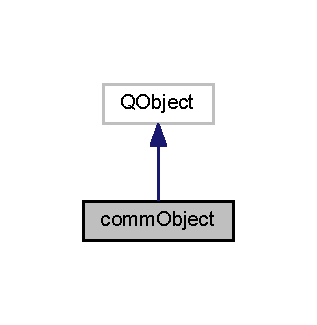
\includegraphics[width=152pt]{classcomm_object__inherit__graph}
\end{center}
\end{figure}


Collaboration diagram for comm\+Object\+:\nopagebreak
\begin{figure}[H]
\begin{center}
\leavevmode
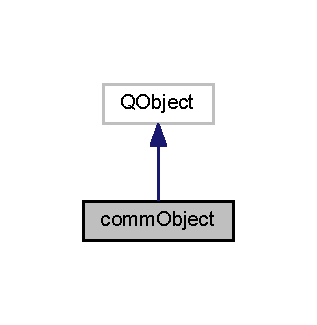
\includegraphics[width=152pt]{classcomm_object__coll__graph}
\end{center}
\end{figure}
\subsection*{Signals}
\begin{DoxyCompactItemize}
\item 
void \hyperlink{classcomm_object_adccf5b5946d35d5cf6d76f367f93e335}{status\+Changed} (Q\+String new\+Text)
\begin{DoxyCompactList}\small\item\em /$<$ S\+I\+G\+N\+AL 0 \end{DoxyCompactList}\item 
void \hyperlink{classcomm_object_a3828eab6be234f6216a6f80a6a82e41e}{image\+Changed} (Q\+Pixmap image)
\begin{DoxyCompactList}\small\item\em /$<$ S\+I\+G\+N\+AL 1 \end{DoxyCompactList}\item 
void \hyperlink{classcomm_object_a72620fe1bac16309baf6d148644edaf9}{log\+Added} (Q\+String Log\+Text)
\begin{DoxyCompactList}\small\item\em /$<$ S\+I\+G\+N\+AL 2 \end{DoxyCompactList}\item 
void \hyperlink{classcomm_object_af2304085624c26230e9d930d616e3e19}{log\+Cleared} ()
\begin{DoxyCompactList}\small\item\em /$<$ S\+I\+G\+N\+AL 3 \end{DoxyCompactList}\item 
void \hyperlink{classcomm_object_af369de87a7f2c9b7170223bedd6c08d9}{P3\+Penabled} (bool value)
\begin{DoxyCompactList}\small\item\em /$<$ S\+I\+G\+N\+AL 4 \end{DoxyCompactList}\item 
void \hyperlink{classcomm_object_a6039d306f25a6b46c78942edf9cee662}{progress\+Updated} (int value)
\begin{DoxyCompactList}\small\item\em /$<$ S\+I\+G\+N\+AL 5 \end{DoxyCompactList}\end{DoxyCompactItemize}
\subsection*{Public Member Functions}
\begin{DoxyCompactItemize}
\item 
void \hyperlink{classcomm_object_a1f4b8dd22ecc46bab619f6b1fe1a5144}{change\+Status} (Q\+String new\+Text)
\item 
void \hyperlink{classcomm_object_a6f81522c2aa1668fa402f08710e6206b}{change\+Image} (Q\+Pixmap image)
\item 
void \hyperlink{classcomm_object_aec354c7099b3039083cc4224e071e022}{add\+Log} (Q\+String Log\+Text)
\item 
void \hyperlink{classcomm_object_a785f776d16f1871786bb88482fc4dd1f}{clear\+Log} ()
\item 
void \hyperlink{classcomm_object_a7552116eb5e18c49c6dcf943de29af7a}{enable\+P3P} (bool value)
\item 
void \hyperlink{classcomm_object_acfc97f4310e2b7d841ecb8cf8be0088e}{progress\+Update} (int value)
\end{DoxyCompactItemize}


\subsection{Member Function Documentation}
\mbox{\Hypertarget{classcomm_object_aec354c7099b3039083cc4224e071e022}\label{classcomm_object_aec354c7099b3039083cc4224e071e022}} 
\index{comm\+Object@{comm\+Object}!add\+Log@{add\+Log}}
\index{add\+Log@{add\+Log}!comm\+Object@{comm\+Object}}
\subsubsection{\texorpdfstring{add\+Log()}{addLog()}}
{\footnotesize\ttfamily void comm\+Object\+::add\+Log (\begin{DoxyParamCaption}\item[{Q\+String}]{Log\+Text }\end{DoxyParamCaption})}

Here is the caller graph for this function\+:\nopagebreak
\begin{figure}[H]
\begin{center}
\leavevmode
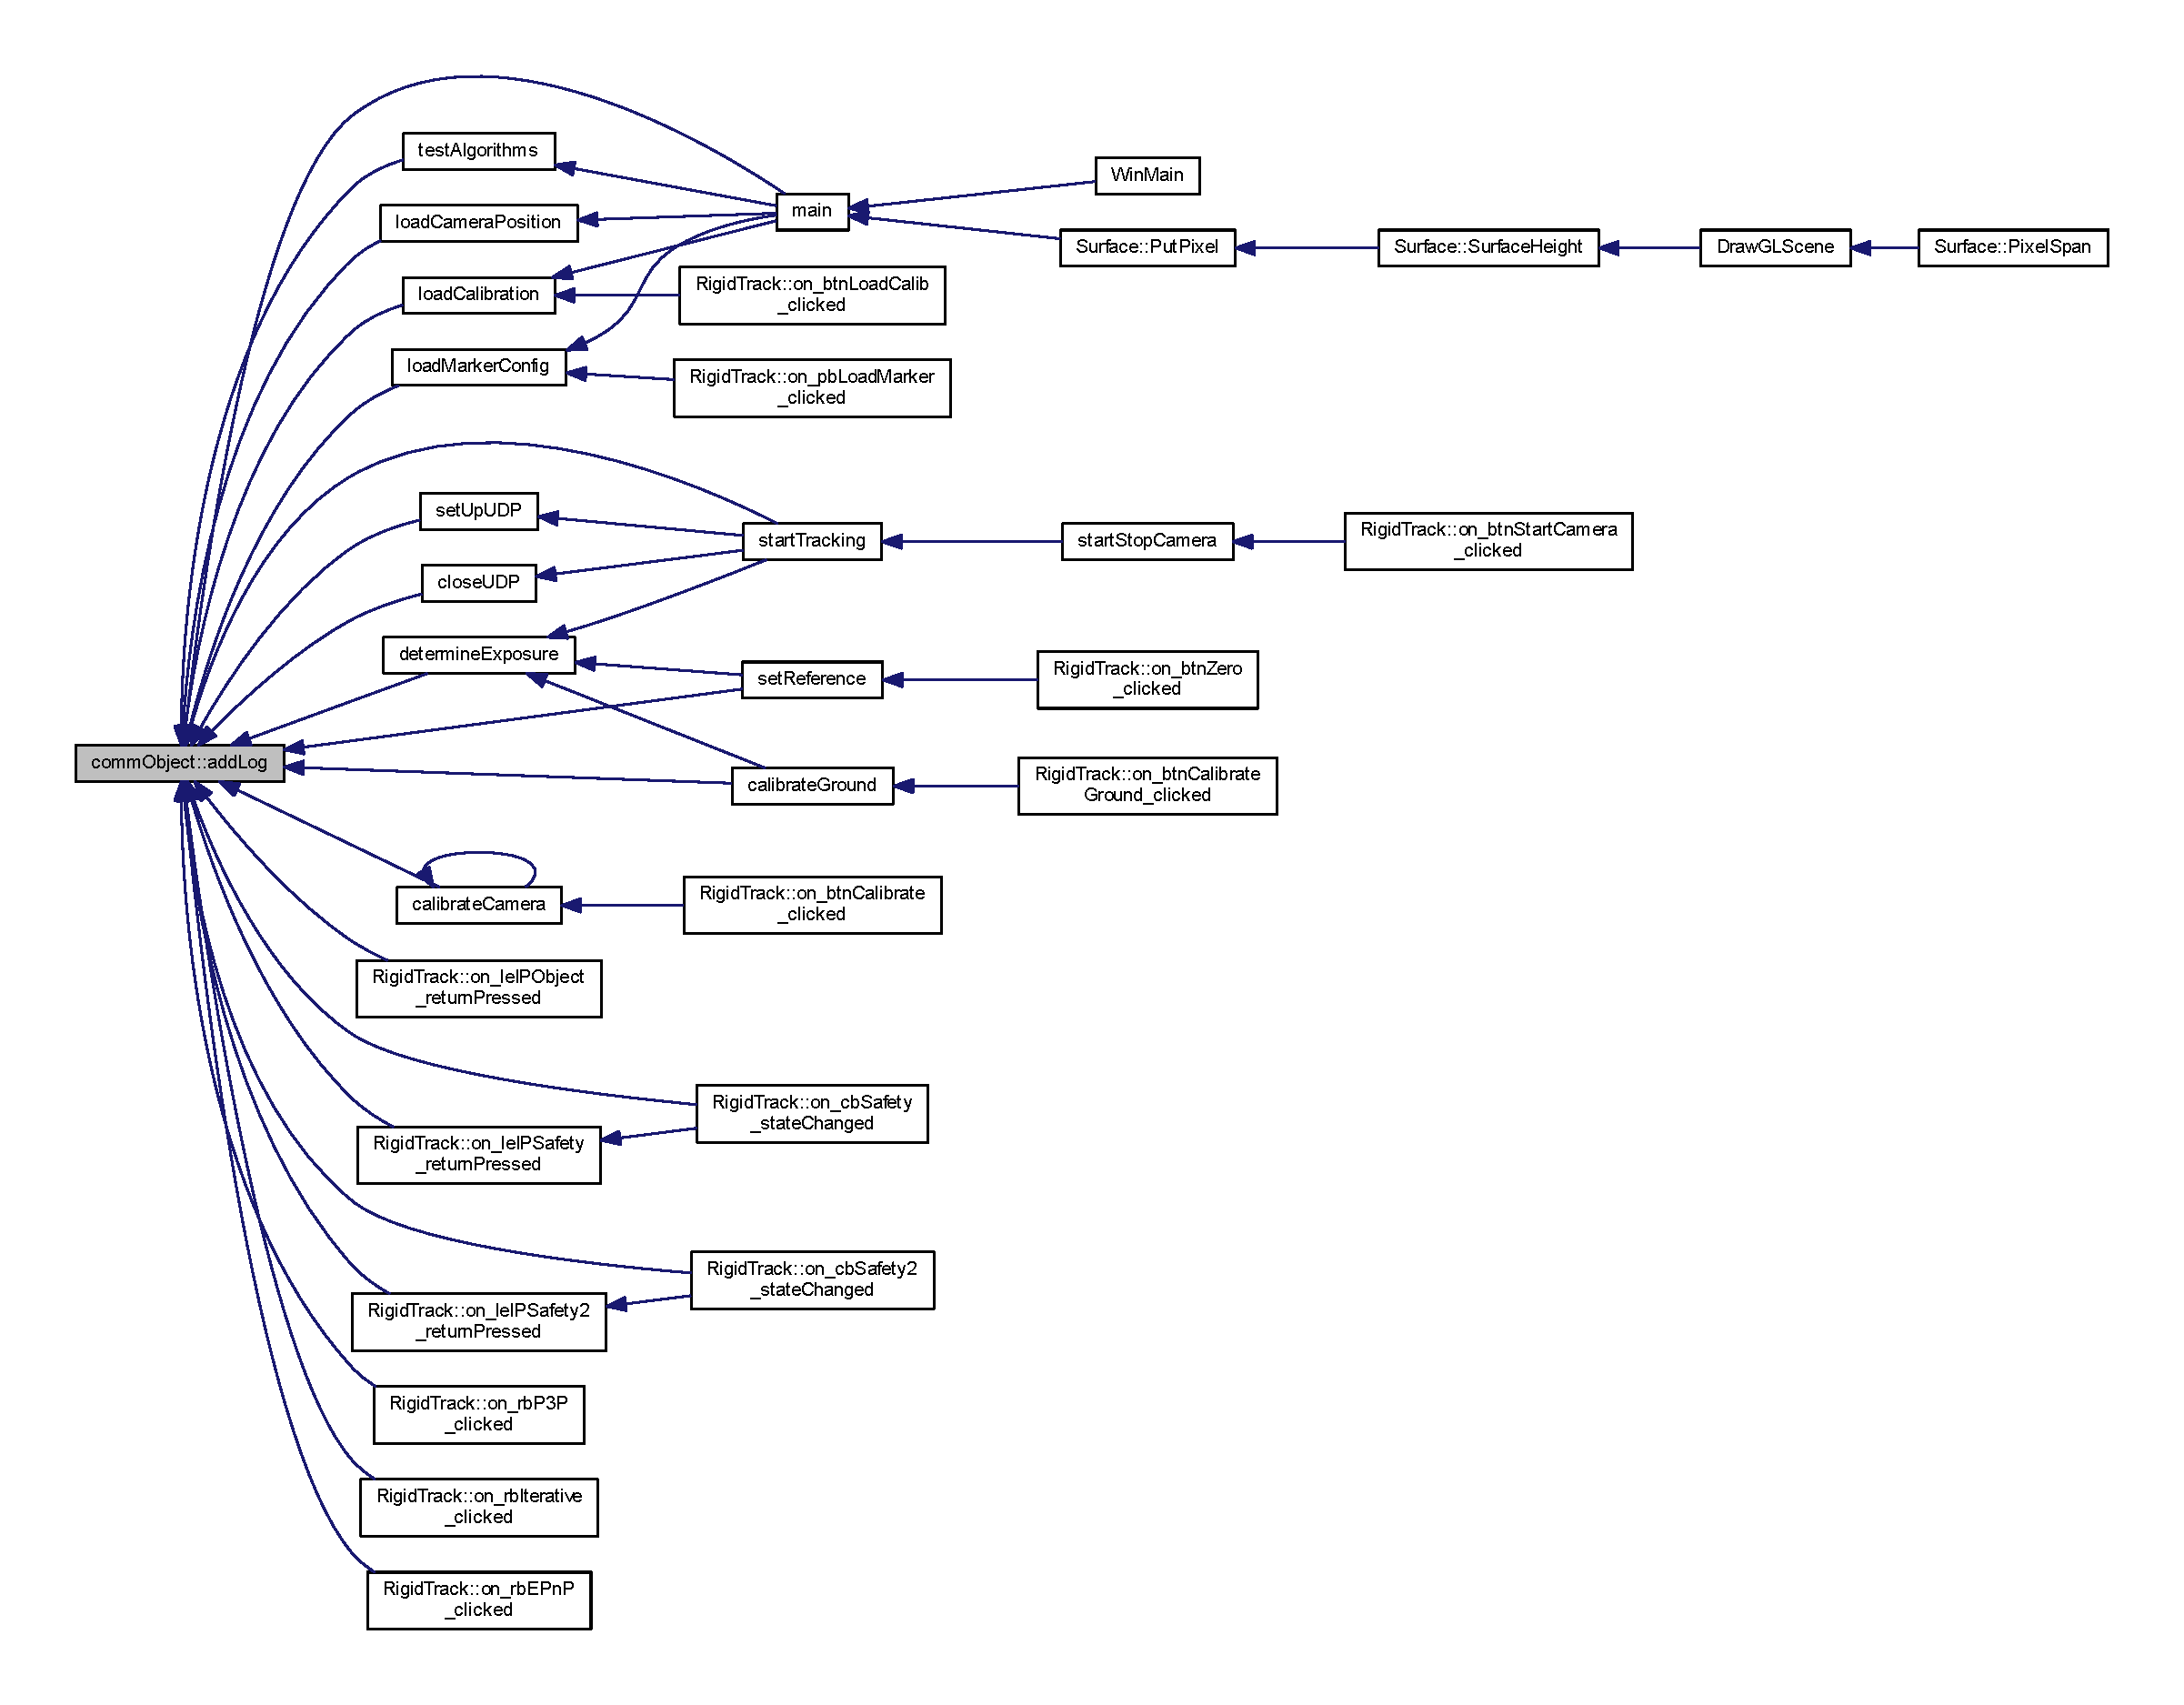
\includegraphics[width=350pt]{classcomm_object_aec354c7099b3039083cc4224e071e022_icgraph}
\end{center}
\end{figure}
\mbox{\Hypertarget{classcomm_object_a6f81522c2aa1668fa402f08710e6206b}\label{classcomm_object_a6f81522c2aa1668fa402f08710e6206b}} 
\index{comm\+Object@{comm\+Object}!change\+Image@{change\+Image}}
\index{change\+Image@{change\+Image}!comm\+Object@{comm\+Object}}
\subsubsection{\texorpdfstring{change\+Image()}{changeImage()}}
{\footnotesize\ttfamily void comm\+Object\+::change\+Image (\begin{DoxyParamCaption}\item[{Q\+Pixmap}]{image }\end{DoxyParamCaption})}

Here is the caller graph for this function\+:\nopagebreak
\begin{figure}[H]
\begin{center}
\leavevmode
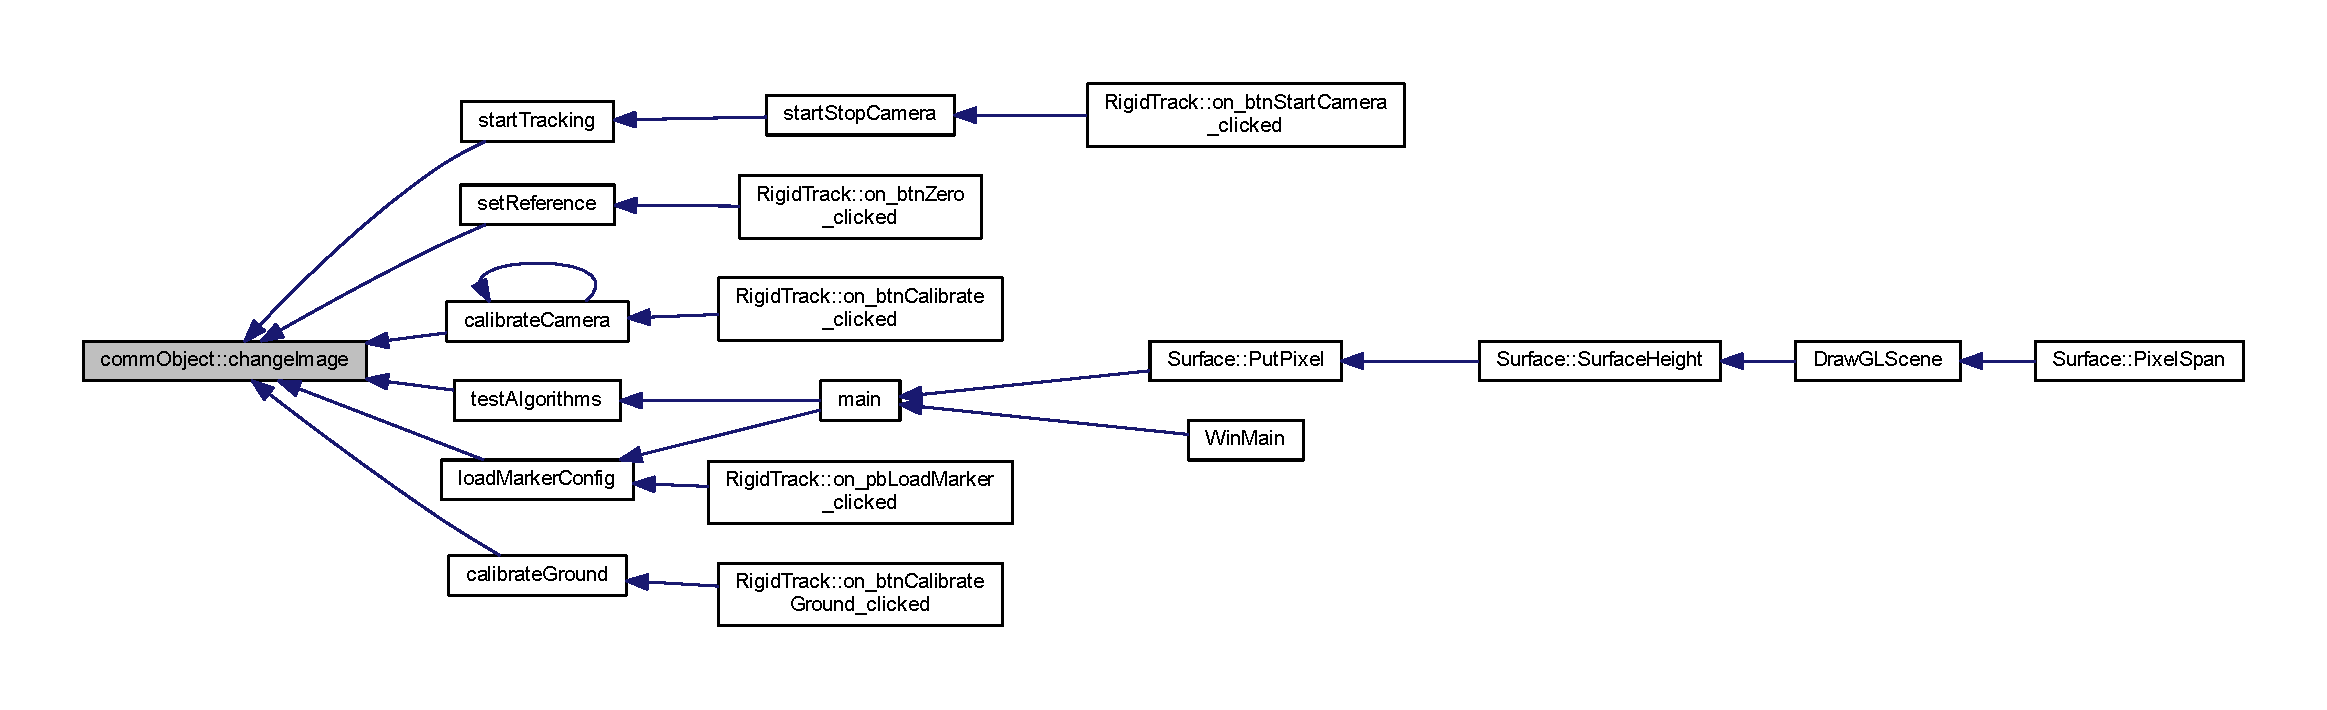
\includegraphics[width=350pt]{classcomm_object_a6f81522c2aa1668fa402f08710e6206b_icgraph}
\end{center}
\end{figure}
\mbox{\Hypertarget{classcomm_object_a1f4b8dd22ecc46bab619f6b1fe1a5144}\label{classcomm_object_a1f4b8dd22ecc46bab619f6b1fe1a5144}} 
\index{comm\+Object@{comm\+Object}!change\+Status@{change\+Status}}
\index{change\+Status@{change\+Status}!comm\+Object@{comm\+Object}}
\subsubsection{\texorpdfstring{change\+Status()}{changeStatus()}}
{\footnotesize\ttfamily void comm\+Object\+::change\+Status (\begin{DoxyParamCaption}\item[{Q\+String}]{new\+Text }\end{DoxyParamCaption})}

Here is the caller graph for this function\+:\nopagebreak
\begin{figure}[H]
\begin{center}
\leavevmode
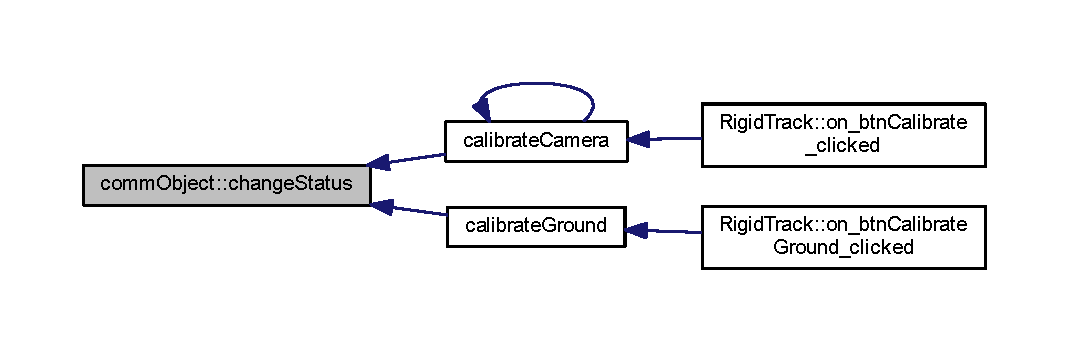
\includegraphics[width=350pt]{classcomm_object_a1f4b8dd22ecc46bab619f6b1fe1a5144_icgraph}
\end{center}
\end{figure}
\mbox{\Hypertarget{classcomm_object_a785f776d16f1871786bb88482fc4dd1f}\label{classcomm_object_a785f776d16f1871786bb88482fc4dd1f}} 
\index{comm\+Object@{comm\+Object}!clear\+Log@{clear\+Log}}
\index{clear\+Log@{clear\+Log}!comm\+Object@{comm\+Object}}
\subsubsection{\texorpdfstring{clear\+Log()}{clearLog()}}
{\footnotesize\ttfamily void comm\+Object\+::clear\+Log (\begin{DoxyParamCaption}{ }\end{DoxyParamCaption})}

\mbox{\Hypertarget{classcomm_object_a7552116eb5e18c49c6dcf943de29af7a}\label{classcomm_object_a7552116eb5e18c49c6dcf943de29af7a}} 
\index{comm\+Object@{comm\+Object}!enable\+P3P@{enable\+P3P}}
\index{enable\+P3P@{enable\+P3P}!comm\+Object@{comm\+Object}}
\subsubsection{\texorpdfstring{enable\+P3\+P()}{enableP3P()}}
{\footnotesize\ttfamily void comm\+Object\+::enable\+P3P (\begin{DoxyParamCaption}\item[{bool}]{value }\end{DoxyParamCaption})}

Here is the caller graph for this function\+:\nopagebreak
\begin{figure}[H]
\begin{center}
\leavevmode
\includegraphics[width=350pt]{classcomm_object_a7552116eb5e18c49c6dcf943de29af7a_icgraph}
\end{center}
\end{figure}
\mbox{\Hypertarget{classcomm_object_a3828eab6be234f6216a6f80a6a82e41e}\label{classcomm_object_a3828eab6be234f6216a6f80a6a82e41e}} 
\index{comm\+Object@{comm\+Object}!image\+Changed@{image\+Changed}}
\index{image\+Changed@{image\+Changed}!comm\+Object@{comm\+Object}}
\subsubsection{\texorpdfstring{image\+Changed}{imageChanged}}
{\footnotesize\ttfamily void comm\+Object\+::image\+Changed (\begin{DoxyParamCaption}\item[{Q\+Pixmap}]{image }\end{DoxyParamCaption})\hspace{0.3cm}{\ttfamily [signal]}}



/$<$ S\+I\+G\+N\+AL 1 

Here is the caller graph for this function\+:\nopagebreak
\begin{figure}[H]
\begin{center}
\leavevmode
\includegraphics[width=350pt]{classcomm_object_a3828eab6be234f6216a6f80a6a82e41e_icgraph}
\end{center}
\end{figure}
\mbox{\Hypertarget{classcomm_object_a72620fe1bac16309baf6d148644edaf9}\label{classcomm_object_a72620fe1bac16309baf6d148644edaf9}} 
\index{comm\+Object@{comm\+Object}!log\+Added@{log\+Added}}
\index{log\+Added@{log\+Added}!comm\+Object@{comm\+Object}}
\subsubsection{\texorpdfstring{log\+Added}{logAdded}}
{\footnotesize\ttfamily void comm\+Object\+::log\+Added (\begin{DoxyParamCaption}\item[{Q\+String}]{Log\+Text }\end{DoxyParamCaption})\hspace{0.3cm}{\ttfamily [signal]}}



/$<$ S\+I\+G\+N\+AL 2 

Here is the caller graph for this function\+:\nopagebreak
\begin{figure}[H]
\begin{center}
\leavevmode
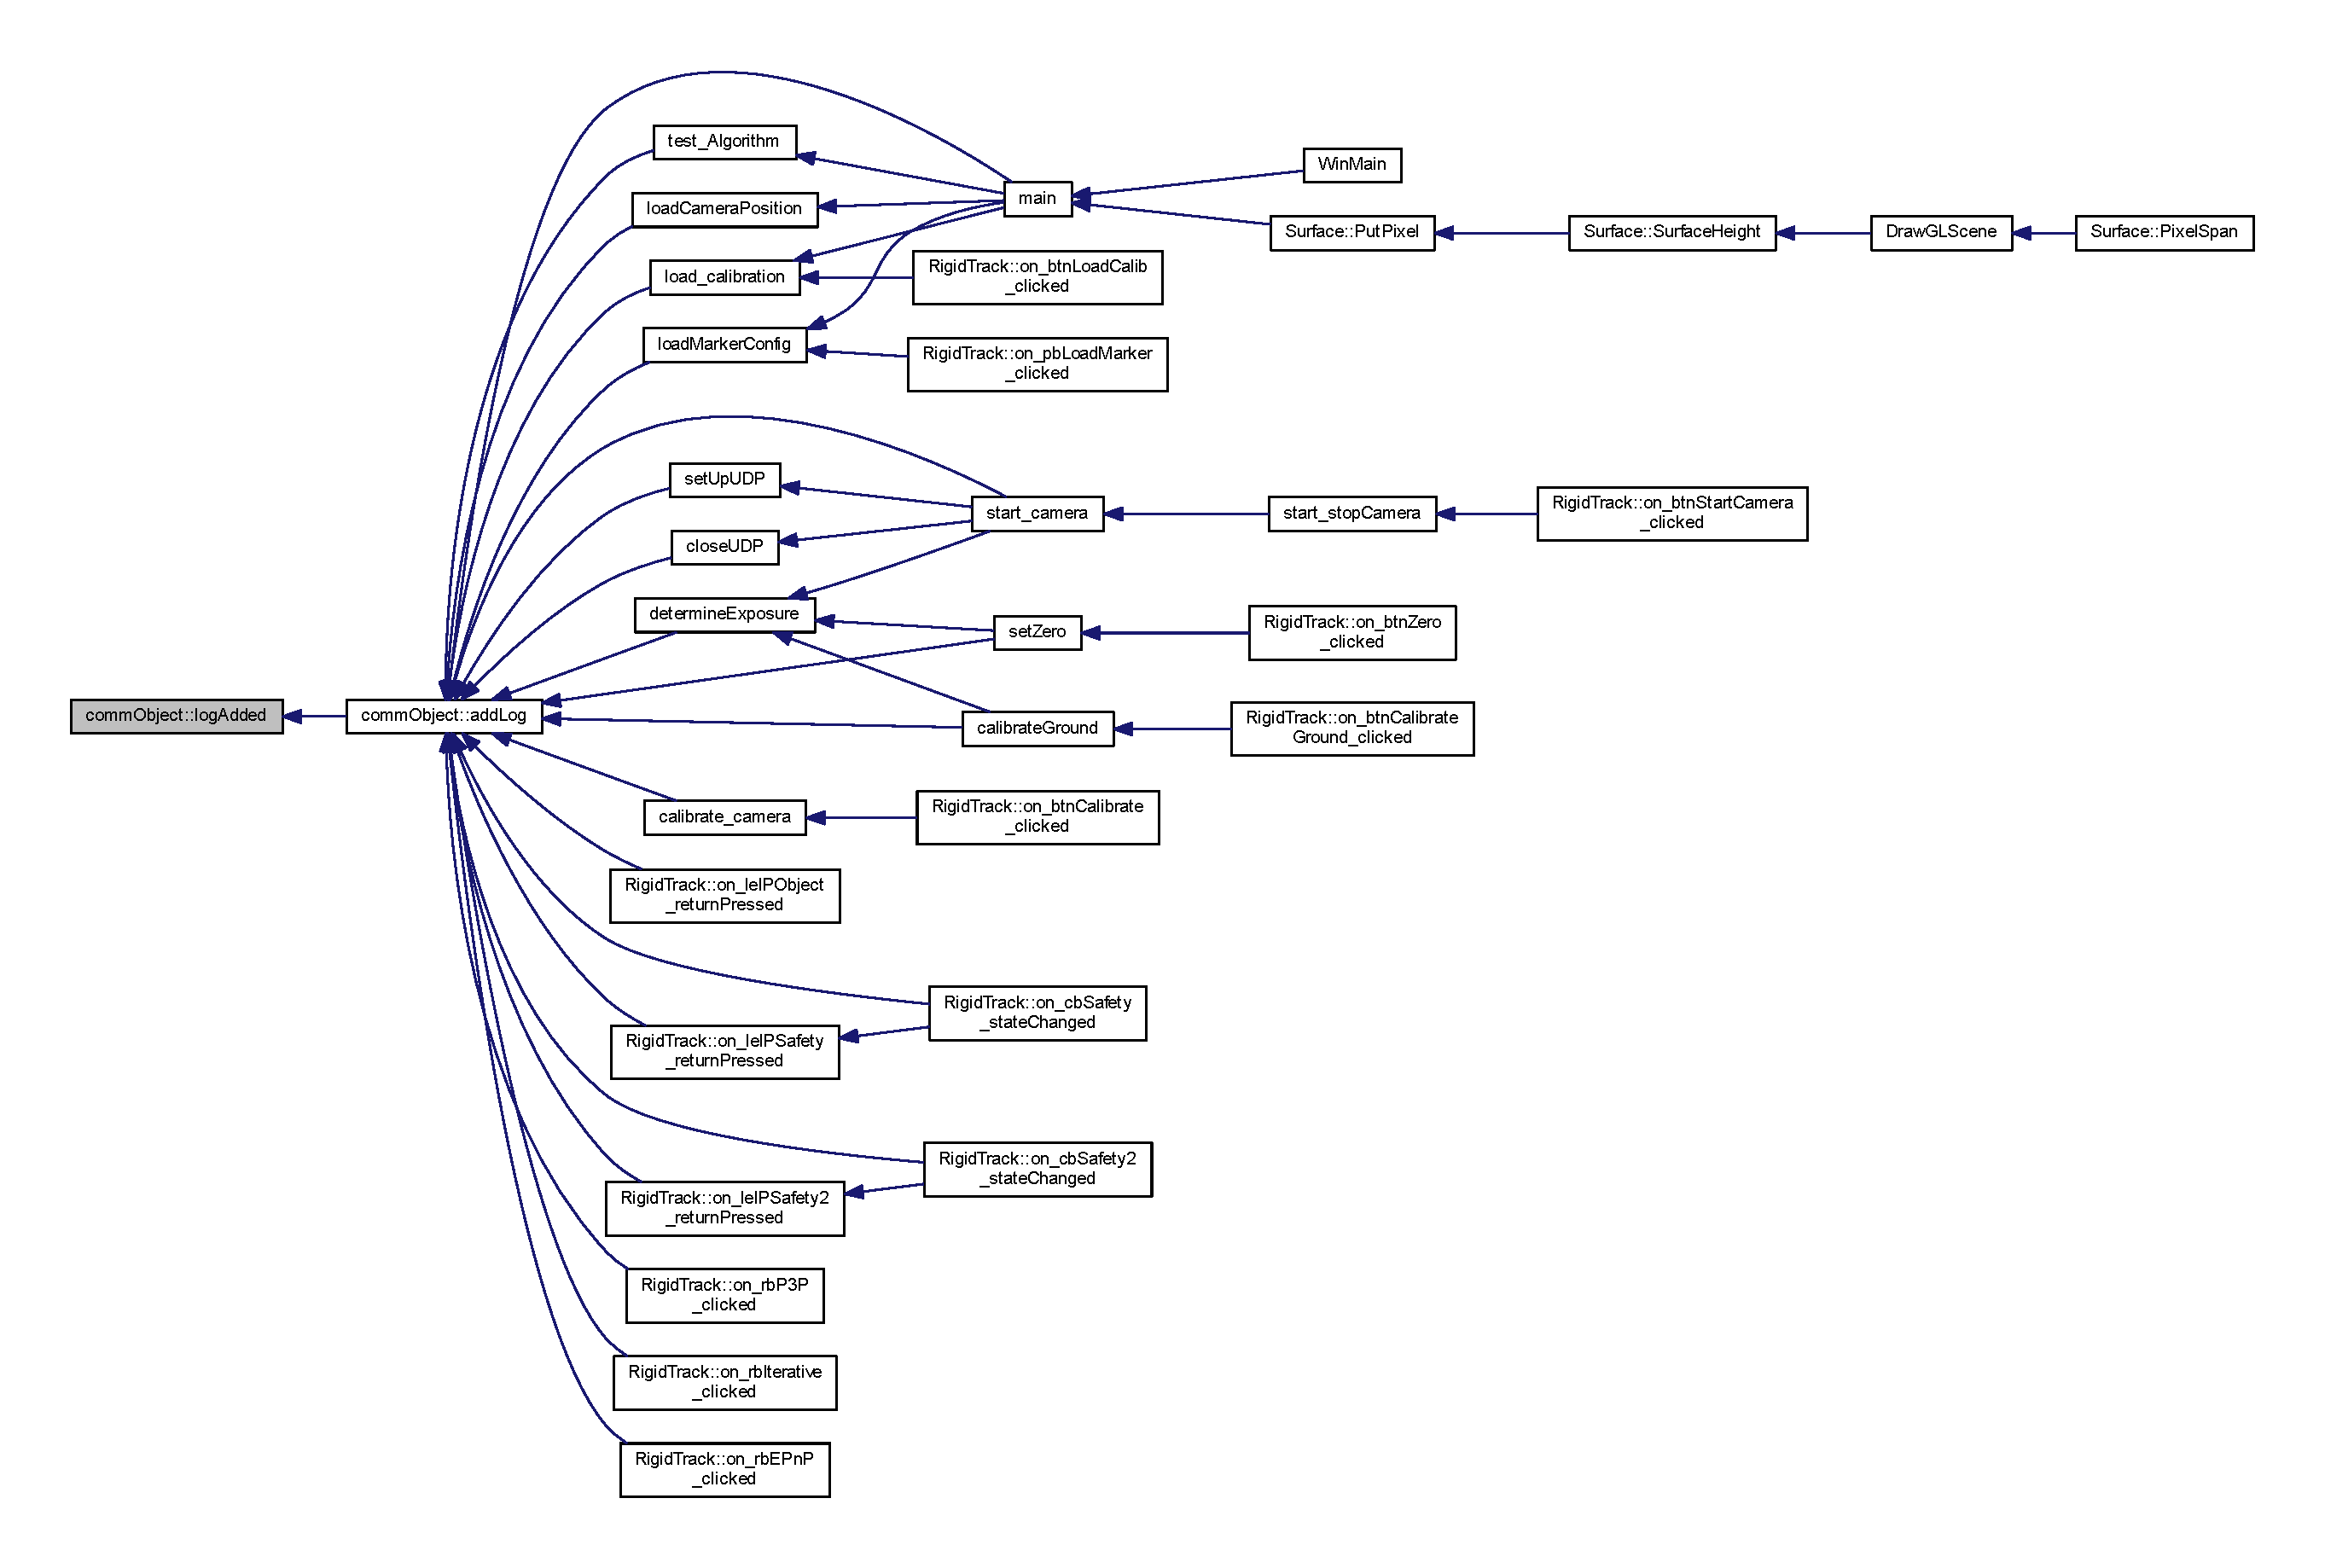
\includegraphics[width=350pt]{classcomm_object_a72620fe1bac16309baf6d148644edaf9_icgraph}
\end{center}
\end{figure}
\mbox{\Hypertarget{classcomm_object_af2304085624c26230e9d930d616e3e19}\label{classcomm_object_af2304085624c26230e9d930d616e3e19}} 
\index{comm\+Object@{comm\+Object}!log\+Cleared@{log\+Cleared}}
\index{log\+Cleared@{log\+Cleared}!comm\+Object@{comm\+Object}}
\subsubsection{\texorpdfstring{log\+Cleared}{logCleared}}
{\footnotesize\ttfamily void comm\+Object\+::log\+Cleared (\begin{DoxyParamCaption}{ }\end{DoxyParamCaption})\hspace{0.3cm}{\ttfamily [signal]}}



/$<$ S\+I\+G\+N\+AL 3 

Here is the caller graph for this function\+:\nopagebreak
\begin{figure}[H]
\begin{center}
\leavevmode
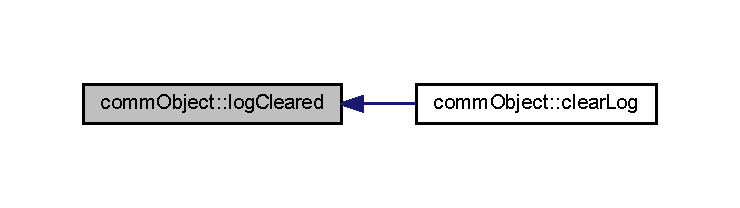
\includegraphics[width=350pt]{classcomm_object_af2304085624c26230e9d930d616e3e19_icgraph}
\end{center}
\end{figure}
\mbox{\Hypertarget{classcomm_object_af369de87a7f2c9b7170223bedd6c08d9}\label{classcomm_object_af369de87a7f2c9b7170223bedd6c08d9}} 
\index{comm\+Object@{comm\+Object}!P3\+Penabled@{P3\+Penabled}}
\index{P3\+Penabled@{P3\+Penabled}!comm\+Object@{comm\+Object}}
\subsubsection{\texorpdfstring{P3\+Penabled}{P3Penabled}}
{\footnotesize\ttfamily void comm\+Object\+::\+P3\+Penabled (\begin{DoxyParamCaption}\item[{bool}]{value }\end{DoxyParamCaption})\hspace{0.3cm}{\ttfamily [signal]}}



/$<$ S\+I\+G\+N\+AL 4 

Here is the caller graph for this function\+:\nopagebreak
\begin{figure}[H]
\begin{center}
\leavevmode
\includegraphics[width=350pt]{classcomm_object_af369de87a7f2c9b7170223bedd6c08d9_icgraph}
\end{center}
\end{figure}
\mbox{\Hypertarget{classcomm_object_acfc97f4310e2b7d841ecb8cf8be0088e}\label{classcomm_object_acfc97f4310e2b7d841ecb8cf8be0088e}} 
\index{comm\+Object@{comm\+Object}!progress\+Update@{progress\+Update}}
\index{progress\+Update@{progress\+Update}!comm\+Object@{comm\+Object}}
\subsubsection{\texorpdfstring{progress\+Update()}{progressUpdate()}}
{\footnotesize\ttfamily void comm\+Object\+::progress\+Update (\begin{DoxyParamCaption}\item[{int}]{value }\end{DoxyParamCaption})}

Here is the caller graph for this function\+:\nopagebreak
\begin{figure}[H]
\begin{center}
\leavevmode
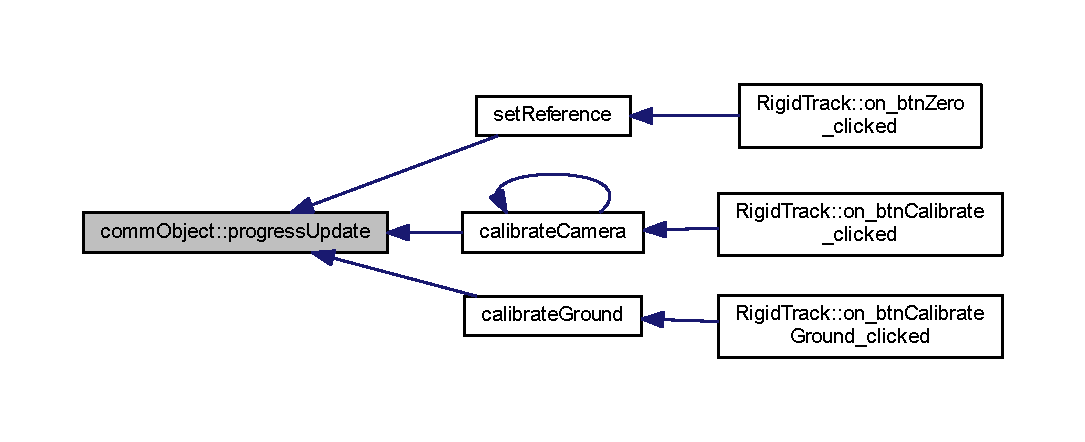
\includegraphics[width=350pt]{classcomm_object_acfc97f4310e2b7d841ecb8cf8be0088e_icgraph}
\end{center}
\end{figure}
\mbox{\Hypertarget{classcomm_object_a6039d306f25a6b46c78942edf9cee662}\label{classcomm_object_a6039d306f25a6b46c78942edf9cee662}} 
\index{comm\+Object@{comm\+Object}!progress\+Updated@{progress\+Updated}}
\index{progress\+Updated@{progress\+Updated}!comm\+Object@{comm\+Object}}
\subsubsection{\texorpdfstring{progress\+Updated}{progressUpdated}}
{\footnotesize\ttfamily void comm\+Object\+::progress\+Updated (\begin{DoxyParamCaption}\item[{int}]{value }\end{DoxyParamCaption})\hspace{0.3cm}{\ttfamily [signal]}}



/$<$ S\+I\+G\+N\+AL 5 

Here is the caller graph for this function\+:\nopagebreak
\begin{figure}[H]
\begin{center}
\leavevmode
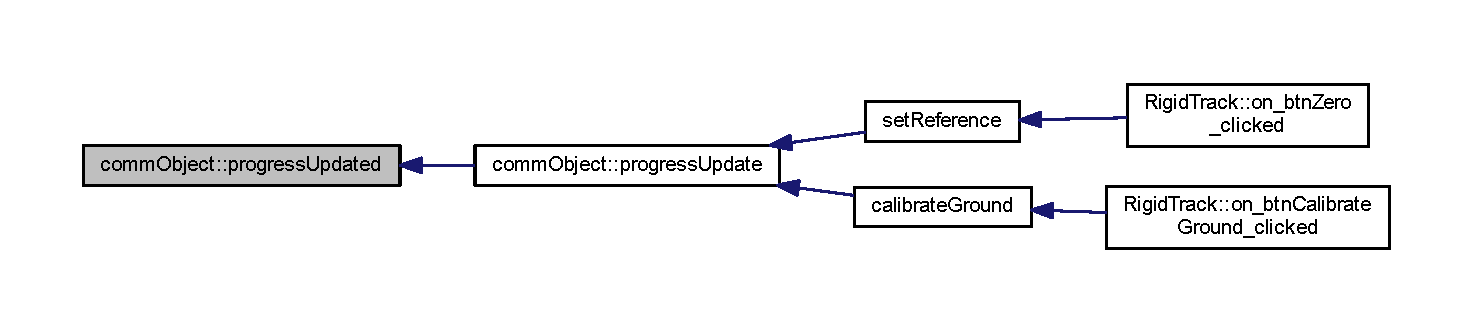
\includegraphics[width=350pt]{classcomm_object_a6039d306f25a6b46c78942edf9cee662_icgraph}
\end{center}
\end{figure}
\mbox{\Hypertarget{classcomm_object_adccf5b5946d35d5cf6d76f367f93e335}\label{classcomm_object_adccf5b5946d35d5cf6d76f367f93e335}} 
\index{comm\+Object@{comm\+Object}!status\+Changed@{status\+Changed}}
\index{status\+Changed@{status\+Changed}!comm\+Object@{comm\+Object}}
\subsubsection{\texorpdfstring{status\+Changed}{statusChanged}}
{\footnotesize\ttfamily void comm\+Object\+::status\+Changed (\begin{DoxyParamCaption}\item[{Q\+String}]{new\+Text }\end{DoxyParamCaption})\hspace{0.3cm}{\ttfamily [signal]}}



/$<$ S\+I\+G\+N\+AL 0 

Here is the caller graph for this function\+:\nopagebreak
\begin{figure}[H]
\begin{center}
\leavevmode
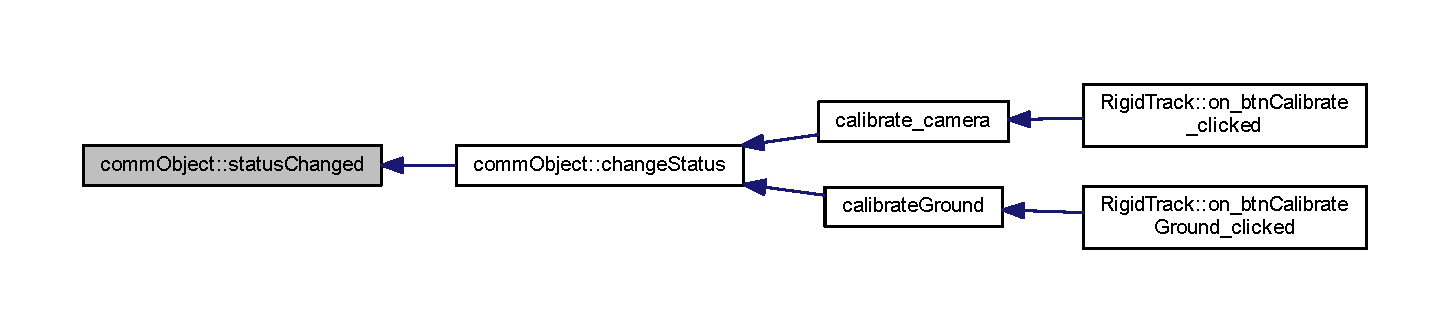
\includegraphics[width=350pt]{classcomm_object_adccf5b5946d35d5cf6d76f367f93e335_icgraph}
\end{center}
\end{figure}


The documentation for this class was generated from the following files\+:\begin{DoxyCompactItemize}
\item 
Rigid\+Track/\hyperlink{communication_8h}{communication.\+h}\item 
Rigid\+Track/\hyperlink{communication_8cpp}{communication.\+cpp}\item 
Rigid\+Track/\+Generated\+Files/\+Debug/\hyperlink{_debug_2moc__communication_8cpp}{moc\+\_\+communication.\+cpp}\end{DoxyCompactItemize}

\hypertarget{class_cv_model_estimator2}{}\section{Cv\+Model\+Estimator2 Class Reference}
\label{class_cv_model_estimator2}\index{Cv\+Model\+Estimator2@{Cv\+Model\+Estimator2}}


{\ttfamily \#include $<$\+\_\+modelest.\+h$>$}

\subsection*{Public Member Functions}
\begin{DoxyCompactItemize}
\item 
\hyperlink{class_cv_model_estimator2_a91cf072d79537808e705a9fa31867da3}{Cv\+Model\+Estimator2} (int \+\_\+model\+Points, Cv\+Size \+\_\+model\+Size, int \+\_\+max\+Basic\+Solutions)
\item 
virtual \hyperlink{class_cv_model_estimator2_a656e12f072058449ca45d785c0eaa02a}{$\sim$\+Cv\+Model\+Estimator2} ()
\item 
virtual int \hyperlink{class_cv_model_estimator2_ac8c9c1586d3334f468d4152c67554adc}{run\+Kernel} (const Cv\+Mat $\ast$m1, const Cv\+Mat $\ast$m2, Cv\+Mat $\ast$model)=0
\item 
virtual bool \hyperlink{class_cv_model_estimator2_a15486b3aea44ad7247924dd1532ce5a8}{run\+L\+Me\+DS} (const Cv\+Mat $\ast$m1, const Cv\+Mat $\ast$m2, Cv\+Mat $\ast$model, Cv\+Mat $\ast$mask, double confidence=0.\+99, int max\+Iters=2000)
\item 
virtual bool \hyperlink{class_cv_model_estimator2_af44a8168c5416e210819c7eea380ac66}{run\+R\+A\+N\+S\+AC} (const Cv\+Mat $\ast$m1, const Cv\+Mat $\ast$m2, Cv\+Mat $\ast$model, Cv\+Mat $\ast$mask, double threshold, double confidence=0.\+99, int max\+Iters=2000)
\item 
virtual bool \hyperlink{class_cv_model_estimator2_a760edefe34027333ccc6c19e74cb46d1}{refine} (const Cv\+Mat $\ast$, const Cv\+Mat $\ast$, Cv\+Mat $\ast$, int)
\item 
virtual void \hyperlink{class_cv_model_estimator2_a4946fc6c99f37e5dae1f68e78e85110d}{set\+Seed} (int64 seed)
\end{DoxyCompactItemize}
\subsection*{Protected Member Functions}
\begin{DoxyCompactItemize}
\item 
virtual void \hyperlink{class_cv_model_estimator2_ae2aa4bbc11e6fc303d81b95daf2795ad}{compute\+Reproj\+Error} (const Cv\+Mat $\ast$m1, const Cv\+Mat $\ast$m2, const Cv\+Mat $\ast$model, Cv\+Mat $\ast$\hyperlink{_import_log_8m_af10dacfa214e2575bb2e0ee407c242e0}{error})=0
\item 
virtual int \hyperlink{class_cv_model_estimator2_a7683a8352f66ba994982493690f418b1}{find\+Inliers} (const Cv\+Mat $\ast$m1, const Cv\+Mat $\ast$m2, const Cv\+Mat $\ast$model, Cv\+Mat $\ast$\hyperlink{_import_log_8m_af10dacfa214e2575bb2e0ee407c242e0}{error}, Cv\+Mat $\ast$mask, double threshold)
\item 
virtual bool \hyperlink{class_cv_model_estimator2_a8a1749e60a02a5cb697425bd2daa35af}{get\+Subset} (const Cv\+Mat $\ast$m1, const Cv\+Mat $\ast$m2, Cv\+Mat $\ast$ms1, Cv\+Mat $\ast$ms2, int max\+Attempts=1000)
\item 
virtual bool \hyperlink{class_cv_model_estimator2_ae149bd480d9b445c66b1c34a351cbb5a}{check\+Subset} (const Cv\+Mat $\ast$ms1, int count)
\end{DoxyCompactItemize}
\subsection*{Protected Attributes}
\begin{DoxyCompactItemize}
\item 
Cv\+R\+NG \hyperlink{class_cv_model_estimator2_a5199037f573a5af1bd9f419e5a64e3e4}{rng}
\item 
int \hyperlink{class_cv_model_estimator2_a7c4067aa8938e61ca4b2674a58ccfe35}{model\+Points}
\item 
Cv\+Size \hyperlink{class_cv_model_estimator2_a93286a6b978450e6363b2403b5da1ff5}{model\+Size}
\item 
int \hyperlink{class_cv_model_estimator2_ac954ec76553da0908f863c48aa82d1ef}{max\+Basic\+Solutions}
\item 
bool \hyperlink{class_cv_model_estimator2_a579cf07784af6c3710ab23aa841cb7d5}{check\+Partial\+Subsets}
\end{DoxyCompactItemize}


\subsection{Constructor \& Destructor Documentation}
\mbox{\Hypertarget{class_cv_model_estimator2_a91cf072d79537808e705a9fa31867da3}\label{class_cv_model_estimator2_a91cf072d79537808e705a9fa31867da3}} 
\index{Cv\+Model\+Estimator2@{Cv\+Model\+Estimator2}!Cv\+Model\+Estimator2@{Cv\+Model\+Estimator2}}
\index{Cv\+Model\+Estimator2@{Cv\+Model\+Estimator2}!Cv\+Model\+Estimator2@{Cv\+Model\+Estimator2}}
\subsubsection{\texorpdfstring{Cv\+Model\+Estimator2()}{CvModelEstimator2()}}
{\footnotesize\ttfamily Cv\+Model\+Estimator2\+::\+Cv\+Model\+Estimator2 (\begin{DoxyParamCaption}\item[{int}]{\+\_\+model\+Points,  }\item[{Cv\+Size}]{\+\_\+model\+Size,  }\item[{int}]{\+\_\+max\+Basic\+Solutions }\end{DoxyParamCaption})}

\mbox{\Hypertarget{class_cv_model_estimator2_a656e12f072058449ca45d785c0eaa02a}\label{class_cv_model_estimator2_a656e12f072058449ca45d785c0eaa02a}} 
\index{Cv\+Model\+Estimator2@{Cv\+Model\+Estimator2}!````~Cv\+Model\+Estimator2@{$\sim$\+Cv\+Model\+Estimator2}}
\index{````~Cv\+Model\+Estimator2@{$\sim$\+Cv\+Model\+Estimator2}!Cv\+Model\+Estimator2@{Cv\+Model\+Estimator2}}
\subsubsection{\texorpdfstring{$\sim$\+Cv\+Model\+Estimator2()}{~CvModelEstimator2()}}
{\footnotesize\ttfamily virtual Cv\+Model\+Estimator2\+::$\sim$\+Cv\+Model\+Estimator2 (\begin{DoxyParamCaption}{ }\end{DoxyParamCaption})\hspace{0.3cm}{\ttfamily [virtual]}}



\subsection{Member Function Documentation}
\mbox{\Hypertarget{class_cv_model_estimator2_ae149bd480d9b445c66b1c34a351cbb5a}\label{class_cv_model_estimator2_ae149bd480d9b445c66b1c34a351cbb5a}} 
\index{Cv\+Model\+Estimator2@{Cv\+Model\+Estimator2}!check\+Subset@{check\+Subset}}
\index{check\+Subset@{check\+Subset}!Cv\+Model\+Estimator2@{Cv\+Model\+Estimator2}}
\subsubsection{\texorpdfstring{check\+Subset()}{checkSubset()}}
{\footnotesize\ttfamily virtual bool Cv\+Model\+Estimator2\+::check\+Subset (\begin{DoxyParamCaption}\item[{const Cv\+Mat $\ast$}]{ms1,  }\item[{int}]{count }\end{DoxyParamCaption})\hspace{0.3cm}{\ttfamily [protected]}, {\ttfamily [virtual]}}

\mbox{\Hypertarget{class_cv_model_estimator2_ae2aa4bbc11e6fc303d81b95daf2795ad}\label{class_cv_model_estimator2_ae2aa4bbc11e6fc303d81b95daf2795ad}} 
\index{Cv\+Model\+Estimator2@{Cv\+Model\+Estimator2}!compute\+Reproj\+Error@{compute\+Reproj\+Error}}
\index{compute\+Reproj\+Error@{compute\+Reproj\+Error}!Cv\+Model\+Estimator2@{Cv\+Model\+Estimator2}}
\subsubsection{\texorpdfstring{compute\+Reproj\+Error()}{computeReprojError()}}
{\footnotesize\ttfamily virtual void Cv\+Model\+Estimator2\+::compute\+Reproj\+Error (\begin{DoxyParamCaption}\item[{const Cv\+Mat $\ast$}]{m1,  }\item[{const Cv\+Mat $\ast$}]{m2,  }\item[{const Cv\+Mat $\ast$}]{model,  }\item[{Cv\+Mat $\ast$}]{error }\end{DoxyParamCaption})\hspace{0.3cm}{\ttfamily [protected]}, {\ttfamily [pure virtual]}}

\mbox{\Hypertarget{class_cv_model_estimator2_a7683a8352f66ba994982493690f418b1}\label{class_cv_model_estimator2_a7683a8352f66ba994982493690f418b1}} 
\index{Cv\+Model\+Estimator2@{Cv\+Model\+Estimator2}!find\+Inliers@{find\+Inliers}}
\index{find\+Inliers@{find\+Inliers}!Cv\+Model\+Estimator2@{Cv\+Model\+Estimator2}}
\subsubsection{\texorpdfstring{find\+Inliers()}{findInliers()}}
{\footnotesize\ttfamily virtual int Cv\+Model\+Estimator2\+::find\+Inliers (\begin{DoxyParamCaption}\item[{const Cv\+Mat $\ast$}]{m1,  }\item[{const Cv\+Mat $\ast$}]{m2,  }\item[{const Cv\+Mat $\ast$}]{model,  }\item[{Cv\+Mat $\ast$}]{error,  }\item[{Cv\+Mat $\ast$}]{mask,  }\item[{double}]{threshold }\end{DoxyParamCaption})\hspace{0.3cm}{\ttfamily [protected]}, {\ttfamily [virtual]}}

\mbox{\Hypertarget{class_cv_model_estimator2_a8a1749e60a02a5cb697425bd2daa35af}\label{class_cv_model_estimator2_a8a1749e60a02a5cb697425bd2daa35af}} 
\index{Cv\+Model\+Estimator2@{Cv\+Model\+Estimator2}!get\+Subset@{get\+Subset}}
\index{get\+Subset@{get\+Subset}!Cv\+Model\+Estimator2@{Cv\+Model\+Estimator2}}
\subsubsection{\texorpdfstring{get\+Subset()}{getSubset()}}
{\footnotesize\ttfamily virtual bool Cv\+Model\+Estimator2\+::get\+Subset (\begin{DoxyParamCaption}\item[{const Cv\+Mat $\ast$}]{m1,  }\item[{const Cv\+Mat $\ast$}]{m2,  }\item[{Cv\+Mat $\ast$}]{ms1,  }\item[{Cv\+Mat $\ast$}]{ms2,  }\item[{int}]{max\+Attempts = {\ttfamily 1000} }\end{DoxyParamCaption})\hspace{0.3cm}{\ttfamily [protected]}, {\ttfamily [virtual]}}

\mbox{\Hypertarget{class_cv_model_estimator2_a760edefe34027333ccc6c19e74cb46d1}\label{class_cv_model_estimator2_a760edefe34027333ccc6c19e74cb46d1}} 
\index{Cv\+Model\+Estimator2@{Cv\+Model\+Estimator2}!refine@{refine}}
\index{refine@{refine}!Cv\+Model\+Estimator2@{Cv\+Model\+Estimator2}}
\subsubsection{\texorpdfstring{refine()}{refine()}}
{\footnotesize\ttfamily virtual bool Cv\+Model\+Estimator2\+::refine (\begin{DoxyParamCaption}\item[{const Cv\+Mat $\ast$}]{,  }\item[{const Cv\+Mat $\ast$}]{,  }\item[{Cv\+Mat $\ast$}]{,  }\item[{int}]{ }\end{DoxyParamCaption})\hspace{0.3cm}{\ttfamily [inline]}, {\ttfamily [virtual]}}

\mbox{\Hypertarget{class_cv_model_estimator2_ac8c9c1586d3334f468d4152c67554adc}\label{class_cv_model_estimator2_ac8c9c1586d3334f468d4152c67554adc}} 
\index{Cv\+Model\+Estimator2@{Cv\+Model\+Estimator2}!run\+Kernel@{run\+Kernel}}
\index{run\+Kernel@{run\+Kernel}!Cv\+Model\+Estimator2@{Cv\+Model\+Estimator2}}
\subsubsection{\texorpdfstring{run\+Kernel()}{runKernel()}}
{\footnotesize\ttfamily virtual int Cv\+Model\+Estimator2\+::run\+Kernel (\begin{DoxyParamCaption}\item[{const Cv\+Mat $\ast$}]{m1,  }\item[{const Cv\+Mat $\ast$}]{m2,  }\item[{Cv\+Mat $\ast$}]{model }\end{DoxyParamCaption})\hspace{0.3cm}{\ttfamily [pure virtual]}}

\mbox{\Hypertarget{class_cv_model_estimator2_a15486b3aea44ad7247924dd1532ce5a8}\label{class_cv_model_estimator2_a15486b3aea44ad7247924dd1532ce5a8}} 
\index{Cv\+Model\+Estimator2@{Cv\+Model\+Estimator2}!run\+L\+Me\+DS@{run\+L\+Me\+DS}}
\index{run\+L\+Me\+DS@{run\+L\+Me\+DS}!Cv\+Model\+Estimator2@{Cv\+Model\+Estimator2}}
\subsubsection{\texorpdfstring{run\+L\+Me\+D\+S()}{runLMeDS()}}
{\footnotesize\ttfamily virtual bool Cv\+Model\+Estimator2\+::run\+L\+Me\+DS (\begin{DoxyParamCaption}\item[{const Cv\+Mat $\ast$}]{m1,  }\item[{const Cv\+Mat $\ast$}]{m2,  }\item[{Cv\+Mat $\ast$}]{model,  }\item[{Cv\+Mat $\ast$}]{mask,  }\item[{double}]{confidence = {\ttfamily 0.99},  }\item[{int}]{max\+Iters = {\ttfamily 2000} }\end{DoxyParamCaption})\hspace{0.3cm}{\ttfamily [virtual]}}

\mbox{\Hypertarget{class_cv_model_estimator2_af44a8168c5416e210819c7eea380ac66}\label{class_cv_model_estimator2_af44a8168c5416e210819c7eea380ac66}} 
\index{Cv\+Model\+Estimator2@{Cv\+Model\+Estimator2}!run\+R\+A\+N\+S\+AC@{run\+R\+A\+N\+S\+AC}}
\index{run\+R\+A\+N\+S\+AC@{run\+R\+A\+N\+S\+AC}!Cv\+Model\+Estimator2@{Cv\+Model\+Estimator2}}
\subsubsection{\texorpdfstring{run\+R\+A\+N\+S\+A\+C()}{runRANSAC()}}
{\footnotesize\ttfamily virtual bool Cv\+Model\+Estimator2\+::run\+R\+A\+N\+S\+AC (\begin{DoxyParamCaption}\item[{const Cv\+Mat $\ast$}]{m1,  }\item[{const Cv\+Mat $\ast$}]{m2,  }\item[{Cv\+Mat $\ast$}]{model,  }\item[{Cv\+Mat $\ast$}]{mask,  }\item[{double}]{threshold,  }\item[{double}]{confidence = {\ttfamily 0.99},  }\item[{int}]{max\+Iters = {\ttfamily 2000} }\end{DoxyParamCaption})\hspace{0.3cm}{\ttfamily [virtual]}}

\mbox{\Hypertarget{class_cv_model_estimator2_a4946fc6c99f37e5dae1f68e78e85110d}\label{class_cv_model_estimator2_a4946fc6c99f37e5dae1f68e78e85110d}} 
\index{Cv\+Model\+Estimator2@{Cv\+Model\+Estimator2}!set\+Seed@{set\+Seed}}
\index{set\+Seed@{set\+Seed}!Cv\+Model\+Estimator2@{Cv\+Model\+Estimator2}}
\subsubsection{\texorpdfstring{set\+Seed()}{setSeed()}}
{\footnotesize\ttfamily virtual void Cv\+Model\+Estimator2\+::set\+Seed (\begin{DoxyParamCaption}\item[{int64}]{seed }\end{DoxyParamCaption})\hspace{0.3cm}{\ttfamily [virtual]}}



\subsection{Member Data Documentation}
\mbox{\Hypertarget{class_cv_model_estimator2_a579cf07784af6c3710ab23aa841cb7d5}\label{class_cv_model_estimator2_a579cf07784af6c3710ab23aa841cb7d5}} 
\index{Cv\+Model\+Estimator2@{Cv\+Model\+Estimator2}!check\+Partial\+Subsets@{check\+Partial\+Subsets}}
\index{check\+Partial\+Subsets@{check\+Partial\+Subsets}!Cv\+Model\+Estimator2@{Cv\+Model\+Estimator2}}
\subsubsection{\texorpdfstring{check\+Partial\+Subsets}{checkPartialSubsets}}
{\footnotesize\ttfamily bool Cv\+Model\+Estimator2\+::check\+Partial\+Subsets\hspace{0.3cm}{\ttfamily [protected]}}

\mbox{\Hypertarget{class_cv_model_estimator2_ac954ec76553da0908f863c48aa82d1ef}\label{class_cv_model_estimator2_ac954ec76553da0908f863c48aa82d1ef}} 
\index{Cv\+Model\+Estimator2@{Cv\+Model\+Estimator2}!max\+Basic\+Solutions@{max\+Basic\+Solutions}}
\index{max\+Basic\+Solutions@{max\+Basic\+Solutions}!Cv\+Model\+Estimator2@{Cv\+Model\+Estimator2}}
\subsubsection{\texorpdfstring{max\+Basic\+Solutions}{maxBasicSolutions}}
{\footnotesize\ttfamily int Cv\+Model\+Estimator2\+::max\+Basic\+Solutions\hspace{0.3cm}{\ttfamily [protected]}}

\mbox{\Hypertarget{class_cv_model_estimator2_a7c4067aa8938e61ca4b2674a58ccfe35}\label{class_cv_model_estimator2_a7c4067aa8938e61ca4b2674a58ccfe35}} 
\index{Cv\+Model\+Estimator2@{Cv\+Model\+Estimator2}!model\+Points@{model\+Points}}
\index{model\+Points@{model\+Points}!Cv\+Model\+Estimator2@{Cv\+Model\+Estimator2}}
\subsubsection{\texorpdfstring{model\+Points}{modelPoints}}
{\footnotesize\ttfamily int Cv\+Model\+Estimator2\+::model\+Points\hspace{0.3cm}{\ttfamily [protected]}}

\mbox{\Hypertarget{class_cv_model_estimator2_a93286a6b978450e6363b2403b5da1ff5}\label{class_cv_model_estimator2_a93286a6b978450e6363b2403b5da1ff5}} 
\index{Cv\+Model\+Estimator2@{Cv\+Model\+Estimator2}!model\+Size@{model\+Size}}
\index{model\+Size@{model\+Size}!Cv\+Model\+Estimator2@{Cv\+Model\+Estimator2}}
\subsubsection{\texorpdfstring{model\+Size}{modelSize}}
{\footnotesize\ttfamily Cv\+Size Cv\+Model\+Estimator2\+::model\+Size\hspace{0.3cm}{\ttfamily [protected]}}

\mbox{\Hypertarget{class_cv_model_estimator2_a5199037f573a5af1bd9f419e5a64e3e4}\label{class_cv_model_estimator2_a5199037f573a5af1bd9f419e5a64e3e4}} 
\index{Cv\+Model\+Estimator2@{Cv\+Model\+Estimator2}!rng@{rng}}
\index{rng@{rng}!Cv\+Model\+Estimator2@{Cv\+Model\+Estimator2}}
\subsubsection{\texorpdfstring{rng}{rng}}
{\footnotesize\ttfamily Cv\+R\+NG Cv\+Model\+Estimator2\+::rng\hspace{0.3cm}{\ttfamily [protected]}}



The documentation for this class was generated from the following file\+:\begin{DoxyCompactItemize}
\item 
Rigid\+Track/\hyperlink{__modelest_8h}{\+\_\+modelest.\+h}\end{DoxyCompactItemize}

\hypertarget{structqt__meta__stringdata__comm_object__t}{}\section{qt\+\_\+meta\+\_\+stringdata\+\_\+comm\+Object\+\_\+t Struct Reference}
\label{structqt__meta__stringdata__comm_object__t}\index{qt\+\_\+meta\+\_\+stringdata\+\_\+comm\+Object\+\_\+t@{qt\+\_\+meta\+\_\+stringdata\+\_\+comm\+Object\+\_\+t}}
\subsection*{Public Attributes}
\begin{DoxyCompactItemize}
\item 
Q\+Byte\+Array\+Data \hyperlink{structqt__meta__stringdata__comm_object__t_ab43768190379f38a6c0c23931d8c16ba}{data} \mbox{[}12\mbox{]}
\item 
char \hyperlink{structqt__meta__stringdata__comm_object__t_a6206d59bc929b76a102101c37f263f52}{stringdata0} \mbox{[}114\mbox{]}
\end{DoxyCompactItemize}


\subsection{Detailed Description}


Definition at line 21 of file moc\+\_\+communication.\+cpp.



\subsection{Member Data Documentation}
\mbox{\Hypertarget{structqt__meta__stringdata__comm_object__t_ab43768190379f38a6c0c23931d8c16ba}\label{structqt__meta__stringdata__comm_object__t_ab43768190379f38a6c0c23931d8c16ba}} 
\index{qt\+\_\+meta\+\_\+stringdata\+\_\+comm\+Object\+\_\+t@{qt\+\_\+meta\+\_\+stringdata\+\_\+comm\+Object\+\_\+t}!data@{data}}
\index{data@{data}!qt\+\_\+meta\+\_\+stringdata\+\_\+comm\+Object\+\_\+t@{qt\+\_\+meta\+\_\+stringdata\+\_\+comm\+Object\+\_\+t}}
\subsubsection{\texorpdfstring{data}{data}}
{\footnotesize\ttfamily Q\+Byte\+Array\+Data qt\+\_\+meta\+\_\+stringdata\+\_\+comm\+Object\+\_\+t\+::data}



Definition at line 22 of file moc\+\_\+communication.\+cpp.

\mbox{\Hypertarget{structqt__meta__stringdata__comm_object__t_a6206d59bc929b76a102101c37f263f52}\label{structqt__meta__stringdata__comm_object__t_a6206d59bc929b76a102101c37f263f52}} 
\index{qt\+\_\+meta\+\_\+stringdata\+\_\+comm\+Object\+\_\+t@{qt\+\_\+meta\+\_\+stringdata\+\_\+comm\+Object\+\_\+t}!stringdata0@{stringdata0}}
\index{stringdata0@{stringdata0}!qt\+\_\+meta\+\_\+stringdata\+\_\+comm\+Object\+\_\+t@{qt\+\_\+meta\+\_\+stringdata\+\_\+comm\+Object\+\_\+t}}
\subsubsection{\texorpdfstring{stringdata0}{stringdata0}}
{\footnotesize\ttfamily char qt\+\_\+meta\+\_\+stringdata\+\_\+comm\+Object\+\_\+t\+::stringdata0}



Definition at line 23 of file moc\+\_\+communication.\+cpp.



The documentation for this struct was generated from the following file\+:\begin{DoxyCompactItemize}
\item 
Rigid\+Track/\+Generated\+Files/\+Debug/\hyperlink{_debug_2moc__communication_8cpp}{moc\+\_\+communication.\+cpp}\end{DoxyCompactItemize}

\hypertarget{structqt__meta__stringdata___rigid_track__t}{}\section{qt\+\_\+meta\+\_\+stringdata\+\_\+\+Rigid\+Track\+\_\+t Struct Reference}
\label{structqt__meta__stringdata___rigid_track__t}\index{qt\+\_\+meta\+\_\+stringdata\+\_\+\+Rigid\+Track\+\_\+t@{qt\+\_\+meta\+\_\+stringdata\+\_\+\+Rigid\+Track\+\_\+t}}
\subsection*{Public Attributes}
\begin{DoxyCompactItemize}
\item 
Q\+Byte\+Array\+Data \hyperlink{structqt__meta__stringdata___rigid_track__t_ab6ce38dcdd6d5162cfc05928307eb564}{data} \mbox{[}34\mbox{]}
\item 
char \hyperlink{structqt__meta__stringdata___rigid_track__t_ac51ec637d23bab4c04f9b97dba465403}{stringdata0} \mbox{[}651\mbox{]}
\end{DoxyCompactItemize}


\subsection{Member Data Documentation}
\mbox{\Hypertarget{structqt__meta__stringdata___rigid_track__t_ab6ce38dcdd6d5162cfc05928307eb564}\label{structqt__meta__stringdata___rigid_track__t_ab6ce38dcdd6d5162cfc05928307eb564}} 
\index{qt\+\_\+meta\+\_\+stringdata\+\_\+\+Rigid\+Track\+\_\+t@{qt\+\_\+meta\+\_\+stringdata\+\_\+\+Rigid\+Track\+\_\+t}!data@{data}}
\index{data@{data}!qt\+\_\+meta\+\_\+stringdata\+\_\+\+Rigid\+Track\+\_\+t@{qt\+\_\+meta\+\_\+stringdata\+\_\+\+Rigid\+Track\+\_\+t}}
\subsubsection{\texorpdfstring{data}{data}}
{\footnotesize\ttfamily Q\+Byte\+Array\+Data qt\+\_\+meta\+\_\+stringdata\+\_\+\+Rigid\+Track\+\_\+t\+::data}

\mbox{\Hypertarget{structqt__meta__stringdata___rigid_track__t_ac51ec637d23bab4c04f9b97dba465403}\label{structqt__meta__stringdata___rigid_track__t_ac51ec637d23bab4c04f9b97dba465403}} 
\index{qt\+\_\+meta\+\_\+stringdata\+\_\+\+Rigid\+Track\+\_\+t@{qt\+\_\+meta\+\_\+stringdata\+\_\+\+Rigid\+Track\+\_\+t}!stringdata0@{stringdata0}}
\index{stringdata0@{stringdata0}!qt\+\_\+meta\+\_\+stringdata\+\_\+\+Rigid\+Track\+\_\+t@{qt\+\_\+meta\+\_\+stringdata\+\_\+\+Rigid\+Track\+\_\+t}}
\subsubsection{\texorpdfstring{stringdata0}{stringdata0}}
{\footnotesize\ttfamily char qt\+\_\+meta\+\_\+stringdata\+\_\+\+Rigid\+Track\+\_\+t\+::stringdata0}



The documentation for this struct was generated from the following file\+:\begin{DoxyCompactItemize}
\item 
Rigid\+Track/\+Generated\+Files/\+Debug/\hyperlink{_debug_2moc___rigid_track_8cpp}{moc\+\_\+\+Rigid\+Track.\+cpp}\end{DoxyCompactItemize}

\hypertarget{class_rigid_track}{}\section{Rigid\+Track Class Reference}
\label{class_rigid_track}\index{Rigid\+Track@{Rigid\+Track}}


{\ttfamily \#include $<$Rigid\+Track.\+h$>$}



Inheritance diagram for Rigid\+Track\+:\nopagebreak
\begin{figure}[H]
\begin{center}
\leavevmode
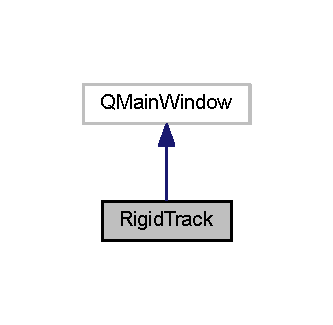
\includegraphics[width=160pt]{class_rigid_track__inherit__graph}
\end{center}
\end{figure}


Collaboration diagram for Rigid\+Track\+:\nopagebreak
\begin{figure}[H]
\begin{center}
\leavevmode
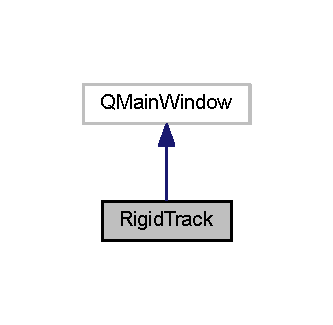
\includegraphics[width=160pt]{class_rigid_track__coll__graph}
\end{center}
\end{figure}
\subsection*{Public Slots}
\begin{DoxyCompactItemize}
\item 
void \hyperlink{class_rigid_track_a2f226856e28868c8bb1854fa16531f60}{on\+\_\+btn\+Start\+Camera\+\_\+clicked} ()
\item 
void \hyperlink{class_rigid_track_afb1a4edcacc818db4ec6bb017dd07e0f}{on\+\_\+btn\+Zero\+\_\+clicked} ()
\item 
void \hyperlink{class_rigid_track_aed2c39da404909142074f7dd2ce75a63}{on\+\_\+btn\+Calibrate\+\_\+clicked} ()
\item 
void \hyperlink{class_rigid_track_a3b0b3835204cad40abdb144d24aefc76}{set\+Image} (Q\+Pixmap image)
\item 
void \hyperlink{class_rigid_track_a6c99fedc157054f4fb752309457fa848}{clear\+Log} ()
\item 
void \hyperlink{class_rigid_track_a9d229d23fdf40b988a1743accb695ea8}{progress\+Update} (int value)
\item 
void \hyperlink{class_rigid_track_a2224d3f6d923a1c7bad356f49d7a4124}{on\+\_\+btn\+Load\+Calib\+\_\+clicked} ()
\item 
void \hyperlink{class_rigid_track_a54a029af74a21f92749e99df7ed847b2}{set\+Log} (Q\+String log\+Text)
\item 
void \hyperlink{class_rigid_track_a72e338d6bf93d0efa3bc503f7ca736c5}{on\+\_\+sb\+Heading\+Offset\+\_\+value\+Changed} (double d)
\item 
void \hyperlink{class_rigid_track_a9f037a061b2577815fc80e5e9f8d46d9}{on\+\_\+le\+I\+P\+Object\+\_\+return\+Pressed} ()
\item 
void \hyperlink{class_rigid_track_aa527ab3a2ddc7b31bf1063260efc9755}{on\+\_\+le\+I\+P\+Safety\+\_\+return\+Pressed} ()
\item 
void \hyperlink{class_rigid_track_a555c536593d659b940de43cd2db8d6c1}{on\+\_\+le\+I\+P\+Safety2\+\_\+return\+Pressed} ()
\item 
void \hyperlink{class_rigid_track_ac1f10ea5ec3f718c152e245a04776454}{on\+\_\+rb\+P3\+P\+\_\+clicked} ()
\item 
void \hyperlink{class_rigid_track_ae5bcdd3fb7203b4a7d1fa97c1460af31}{on\+\_\+rb\+Iterative\+\_\+clicked} ()
\item 
void \hyperlink{class_rigid_track_a19bc46333f946e589184eeed998160da}{on\+\_\+rb\+E\+Pn\+P\+\_\+clicked} ()
\item 
void \hyperlink{class_rigid_track_af14465ac3ad6957b939c63cbae2d7d8c}{on\+\_\+action\+Show\+\_\+\+Help\+\_\+triggered} ()
\item 
void \hyperlink{class_rigid_track_a8f999fa968f4cc9fa548bdc8438b32c4}{on\+\_\+cb\+Safety\+\_\+state\+Changed} (int state)
\item 
void \hyperlink{class_rigid_track_ad6ba1cfe25f18ff0d9f5993aafa36d16}{on\+\_\+cb\+Safety2\+\_\+state\+Changed} (int state)
\item 
void \hyperlink{class_rigid_track_ae5e44de9f4e3cacdd647c0305936b02b}{on\+\_\+dsb\+Dimension\+\_\+value\+Changed} (double d)
\item 
void \hyperlink{class_rigid_track_a217ca3d828c99943ea155e6891264b24}{on\+\_\+sb\+Angle\+\_\+value\+Changed} (int \hyperlink{simpleplot_8m_a81b94ba50b782836960e54bcfa99fc88}{i})
\item 
void \hyperlink{class_rigid_track_ad3e07592fbc1491cdc36dd5e817e1775}{on\+\_\+pb\+Load\+Marker\+\_\+clicked} ()
\item 
void \hyperlink{class_rigid_track_ab347b3edeca55685f4d601549596d44a}{on\+\_\+cb\+Invert\+\_\+state\+Changed} (int state)
\item 
void \hyperlink{class_rigid_track_a39aba14e1c846cb3f1773d9145cf96e1}{enable\+P3P} (bool value)
\item 
void \hyperlink{class_rigid_track_a9a939d6db3d268e75a603cb3d492a91b}{on\+\_\+btn\+Calibrate\+Ground\+\_\+clicked} ()
\item 
void \hyperlink{class_rigid_track_a63a85d33ef48741b0e671ebbbd43083a}{on\+\_\+action\+Open\+\_\+\+Log\+\_\+\+Folder\+\_\+triggered} ()
\item 
void \hyperlink{class_rigid_track_a7d858fcf6c9fe852ee3facfe6588aec1}{on\+\_\+action\+Open\+\_\+\+Installation\+\_\+\+Folder\+\_\+triggered} ()
\end{DoxyCompactItemize}
\subsection*{Public Member Functions}
\begin{DoxyCompactItemize}
\item 
\hyperlink{class_rigid_track_abd3d529ea29b1050439c97c5a5aa8c4b}{Rigid\+Track} (Q\+Widget $\ast$parent=Q\+\_\+\+N\+U\+L\+L\+P\+TR)
\end{DoxyCompactItemize}


\subsection{Constructor \& Destructor Documentation}
\mbox{\Hypertarget{class_rigid_track_abd3d529ea29b1050439c97c5a5aa8c4b}\label{class_rigid_track_abd3d529ea29b1050439c97c5a5aa8c4b}} 
\index{Rigid\+Track@{Rigid\+Track}!Rigid\+Track@{Rigid\+Track}}
\index{Rigid\+Track@{Rigid\+Track}!Rigid\+Track@{Rigid\+Track}}
\subsubsection{\texorpdfstring{Rigid\+Track()}{RigidTrack()}}
{\footnotesize\ttfamily Rigid\+Track\+::\+Rigid\+Track (\begin{DoxyParamCaption}\item[{Q\+Widget $\ast$}]{parent = {\ttfamily Q\+\_\+NULLPTR} }\end{DoxyParamCaption})}

Here is the call graph for this function\+:\nopagebreak
\begin{figure}[H]
\begin{center}
\leavevmode
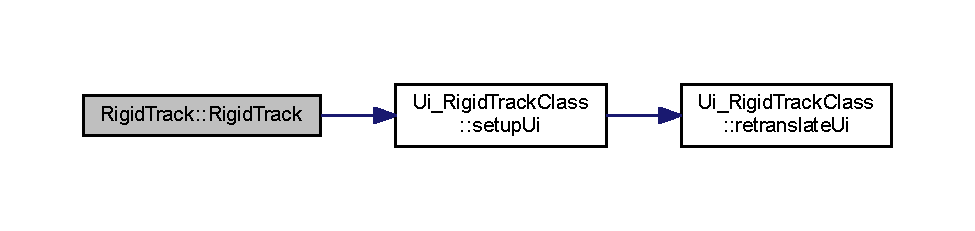
\includegraphics[width=350pt]{class_rigid_track_abd3d529ea29b1050439c97c5a5aa8c4b_cgraph}
\end{center}
\end{figure}


\subsection{Member Function Documentation}
\mbox{\Hypertarget{class_rigid_track_a6c99fedc157054f4fb752309457fa848}\label{class_rigid_track_a6c99fedc157054f4fb752309457fa848}} 
\index{Rigid\+Track@{Rigid\+Track}!clear\+Log@{clear\+Log}}
\index{clear\+Log@{clear\+Log}!Rigid\+Track@{Rigid\+Track}}
\subsubsection{\texorpdfstring{clear\+Log}{clearLog}}
{\footnotesize\ttfamily void Rigid\+Track\+::clear\+Log (\begin{DoxyParamCaption}{ }\end{DoxyParamCaption})\hspace{0.3cm}{\ttfamily [slot]}}

\mbox{\Hypertarget{class_rigid_track_a39aba14e1c846cb3f1773d9145cf96e1}\label{class_rigid_track_a39aba14e1c846cb3f1773d9145cf96e1}} 
\index{Rigid\+Track@{Rigid\+Track}!enable\+P3P@{enable\+P3P}}
\index{enable\+P3P@{enable\+P3P}!Rigid\+Track@{Rigid\+Track}}
\subsubsection{\texorpdfstring{enable\+P3P}{enableP3P}}
{\footnotesize\ttfamily void Rigid\+Track\+::enable\+P3P (\begin{DoxyParamCaption}\item[{bool}]{value }\end{DoxyParamCaption})\hspace{0.3cm}{\ttfamily [slot]}}

\mbox{\Hypertarget{class_rigid_track_a7d858fcf6c9fe852ee3facfe6588aec1}\label{class_rigid_track_a7d858fcf6c9fe852ee3facfe6588aec1}} 
\index{Rigid\+Track@{Rigid\+Track}!on\+\_\+action\+Open\+\_\+\+Installation\+\_\+\+Folder\+\_\+triggered@{on\+\_\+action\+Open\+\_\+\+Installation\+\_\+\+Folder\+\_\+triggered}}
\index{on\+\_\+action\+Open\+\_\+\+Installation\+\_\+\+Folder\+\_\+triggered@{on\+\_\+action\+Open\+\_\+\+Installation\+\_\+\+Folder\+\_\+triggered}!Rigid\+Track@{Rigid\+Track}}
\subsubsection{\texorpdfstring{on\+\_\+action\+Open\+\_\+\+Installation\+\_\+\+Folder\+\_\+triggered}{on\_actionOpen\_Installation\_Folder\_triggered}}
{\footnotesize\ttfamily void Rigid\+Track\+::on\+\_\+action\+Open\+\_\+\+Installation\+\_\+\+Folder\+\_\+triggered (\begin{DoxyParamCaption}{ }\end{DoxyParamCaption})\hspace{0.3cm}{\ttfamily [slot]}}

\mbox{\Hypertarget{class_rigid_track_a63a85d33ef48741b0e671ebbbd43083a}\label{class_rigid_track_a63a85d33ef48741b0e671ebbbd43083a}} 
\index{Rigid\+Track@{Rigid\+Track}!on\+\_\+action\+Open\+\_\+\+Log\+\_\+\+Folder\+\_\+triggered@{on\+\_\+action\+Open\+\_\+\+Log\+\_\+\+Folder\+\_\+triggered}}
\index{on\+\_\+action\+Open\+\_\+\+Log\+\_\+\+Folder\+\_\+triggered@{on\+\_\+action\+Open\+\_\+\+Log\+\_\+\+Folder\+\_\+triggered}!Rigid\+Track@{Rigid\+Track}}
\subsubsection{\texorpdfstring{on\+\_\+action\+Open\+\_\+\+Log\+\_\+\+Folder\+\_\+triggered}{on\_actionOpen\_Log\_Folder\_triggered}}
{\footnotesize\ttfamily void Rigid\+Track\+::on\+\_\+action\+Open\+\_\+\+Log\+\_\+\+Folder\+\_\+triggered (\begin{DoxyParamCaption}{ }\end{DoxyParamCaption})\hspace{0.3cm}{\ttfamily [slot]}}

\mbox{\Hypertarget{class_rigid_track_af14465ac3ad6957b939c63cbae2d7d8c}\label{class_rigid_track_af14465ac3ad6957b939c63cbae2d7d8c}} 
\index{Rigid\+Track@{Rigid\+Track}!on\+\_\+action\+Show\+\_\+\+Help\+\_\+triggered@{on\+\_\+action\+Show\+\_\+\+Help\+\_\+triggered}}
\index{on\+\_\+action\+Show\+\_\+\+Help\+\_\+triggered@{on\+\_\+action\+Show\+\_\+\+Help\+\_\+triggered}!Rigid\+Track@{Rigid\+Track}}
\subsubsection{\texorpdfstring{on\+\_\+action\+Show\+\_\+\+Help\+\_\+triggered}{on\_actionShow\_Help\_triggered}}
{\footnotesize\ttfamily void Rigid\+Track\+::on\+\_\+action\+Show\+\_\+\+Help\+\_\+triggered (\begin{DoxyParamCaption}{ }\end{DoxyParamCaption})\hspace{0.3cm}{\ttfamily [slot]}}

/$<$ append help.\+pdf to the path since this is the documentation in html format

/$<$ open the documentation help file in the standard browser \mbox{\Hypertarget{class_rigid_track_aed2c39da404909142074f7dd2ce75a63}\label{class_rigid_track_aed2c39da404909142074f7dd2ce75a63}} 
\index{Rigid\+Track@{Rigid\+Track}!on\+\_\+btn\+Calibrate\+\_\+clicked@{on\+\_\+btn\+Calibrate\+\_\+clicked}}
\index{on\+\_\+btn\+Calibrate\+\_\+clicked@{on\+\_\+btn\+Calibrate\+\_\+clicked}!Rigid\+Track@{Rigid\+Track}}
\subsubsection{\texorpdfstring{on\+\_\+btn\+Calibrate\+\_\+clicked}{on\_btnCalibrate\_clicked}}
{\footnotesize\ttfamily void Rigid\+Track\+::on\+\_\+btn\+Calibrate\+\_\+clicked (\begin{DoxyParamCaption}{ }\end{DoxyParamCaption})\hspace{0.3cm}{\ttfamily [slot]}}

Here is the call graph for this function\+:\nopagebreak
\begin{figure}[H]
\begin{center}
\leavevmode
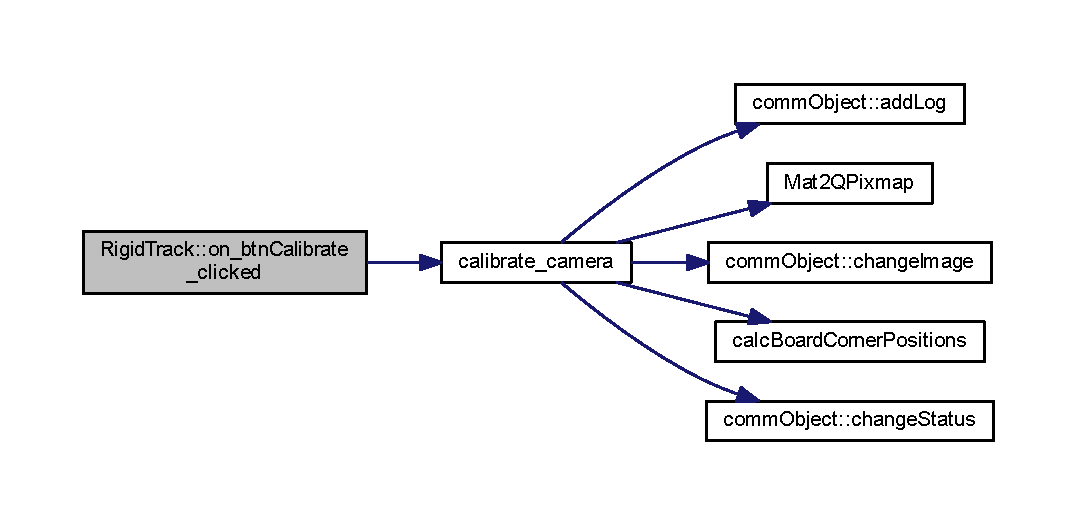
\includegraphics[width=350pt]{class_rigid_track_aed2c39da404909142074f7dd2ce75a63_cgraph}
\end{center}
\end{figure}
\mbox{\Hypertarget{class_rigid_track_a9a939d6db3d268e75a603cb3d492a91b}\label{class_rigid_track_a9a939d6db3d268e75a603cb3d492a91b}} 
\index{Rigid\+Track@{Rigid\+Track}!on\+\_\+btn\+Calibrate\+Ground\+\_\+clicked@{on\+\_\+btn\+Calibrate\+Ground\+\_\+clicked}}
\index{on\+\_\+btn\+Calibrate\+Ground\+\_\+clicked@{on\+\_\+btn\+Calibrate\+Ground\+\_\+clicked}!Rigid\+Track@{Rigid\+Track}}
\subsubsection{\texorpdfstring{on\+\_\+btn\+Calibrate\+Ground\+\_\+clicked}{on\_btnCalibrateGround\_clicked}}
{\footnotesize\ttfamily void Rigid\+Track\+::on\+\_\+btn\+Calibrate\+Ground\+\_\+clicked (\begin{DoxyParamCaption}{ }\end{DoxyParamCaption})\hspace{0.3cm}{\ttfamily [slot]}}

Here is the call graph for this function\+:\nopagebreak
\begin{figure}[H]
\begin{center}
\leavevmode
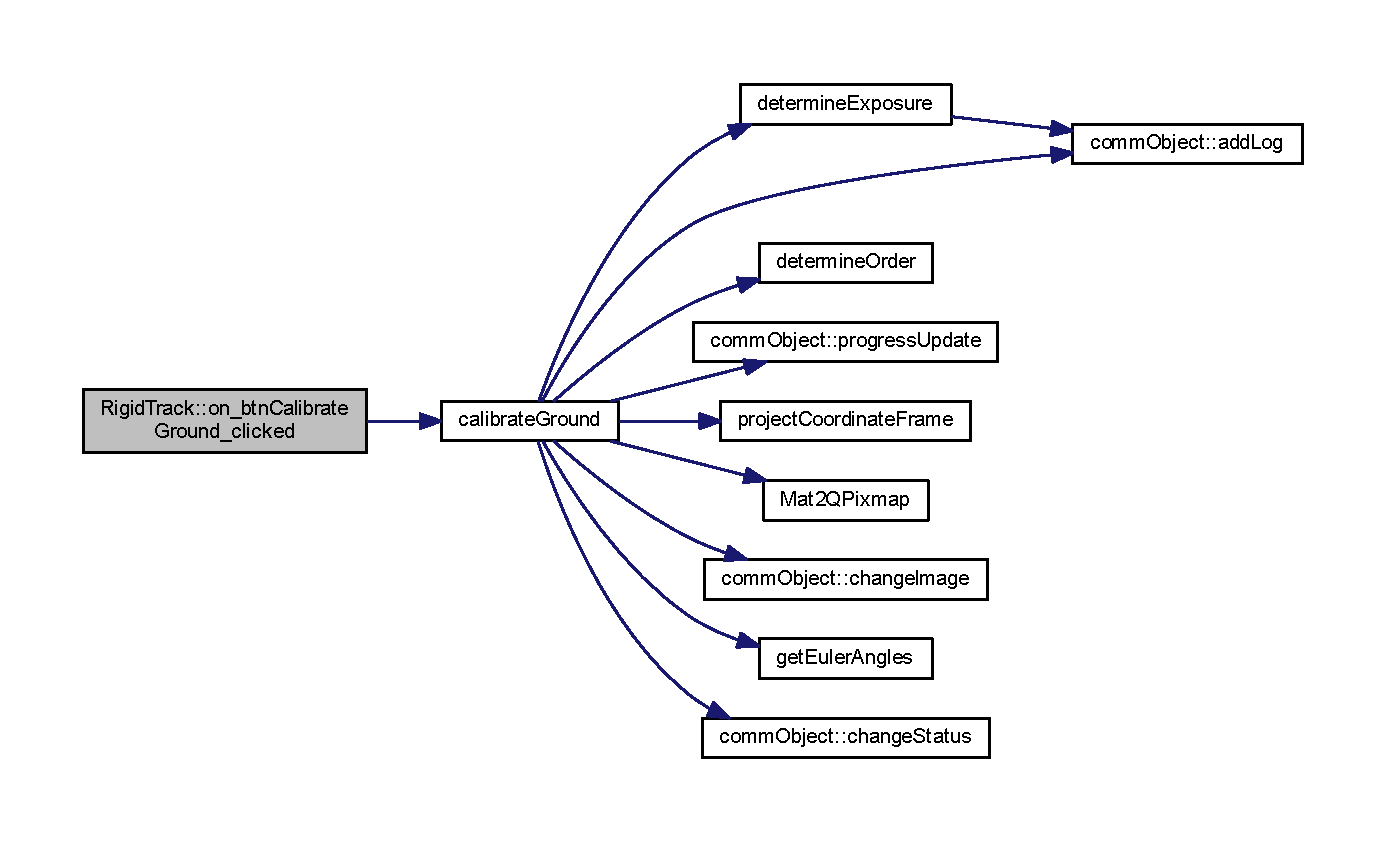
\includegraphics[width=350pt]{class_rigid_track_a9a939d6db3d268e75a603cb3d492a91b_cgraph}
\end{center}
\end{figure}
\mbox{\Hypertarget{class_rigid_track_a2224d3f6d923a1c7bad356f49d7a4124}\label{class_rigid_track_a2224d3f6d923a1c7bad356f49d7a4124}} 
\index{Rigid\+Track@{Rigid\+Track}!on\+\_\+btn\+Load\+Calib\+\_\+clicked@{on\+\_\+btn\+Load\+Calib\+\_\+clicked}}
\index{on\+\_\+btn\+Load\+Calib\+\_\+clicked@{on\+\_\+btn\+Load\+Calib\+\_\+clicked}!Rigid\+Track@{Rigid\+Track}}
\subsubsection{\texorpdfstring{on\+\_\+btn\+Load\+Calib\+\_\+clicked}{on\_btnLoadCalib\_clicked}}
{\footnotesize\ttfamily void Rigid\+Track\+::on\+\_\+btn\+Load\+Calib\+\_\+clicked (\begin{DoxyParamCaption}{ }\end{DoxyParamCaption})\hspace{0.3cm}{\ttfamily [slot]}}

Here is the call graph for this function\+:\nopagebreak
\begin{figure}[H]
\begin{center}
\leavevmode
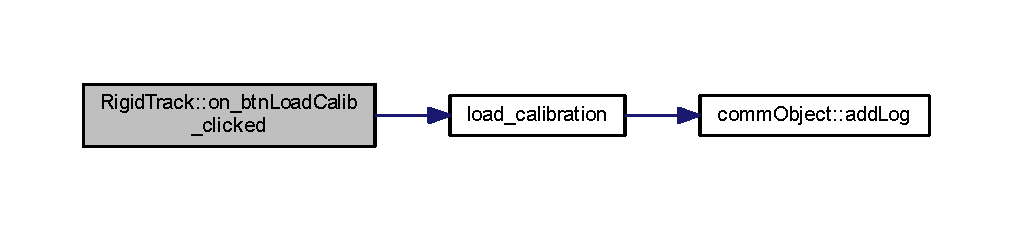
\includegraphics[width=350pt]{class_rigid_track_a2224d3f6d923a1c7bad356f49d7a4124_cgraph}
\end{center}
\end{figure}
\mbox{\Hypertarget{class_rigid_track_a2f226856e28868c8bb1854fa16531f60}\label{class_rigid_track_a2f226856e28868c8bb1854fa16531f60}} 
\index{Rigid\+Track@{Rigid\+Track}!on\+\_\+btn\+Start\+Camera\+\_\+clicked@{on\+\_\+btn\+Start\+Camera\+\_\+clicked}}
\index{on\+\_\+btn\+Start\+Camera\+\_\+clicked@{on\+\_\+btn\+Start\+Camera\+\_\+clicked}!Rigid\+Track@{Rigid\+Track}}
\subsubsection{\texorpdfstring{on\+\_\+btn\+Start\+Camera\+\_\+clicked}{on\_btnStartCamera\_clicked}}
{\footnotesize\ttfamily void Rigid\+Track\+::on\+\_\+btn\+Start\+Camera\+\_\+clicked (\begin{DoxyParamCaption}{ }\end{DoxyParamCaption})\hspace{0.3cm}{\ttfamily [slot]}}

Here is the call graph for this function\+:\nopagebreak
\begin{figure}[H]
\begin{center}
\leavevmode
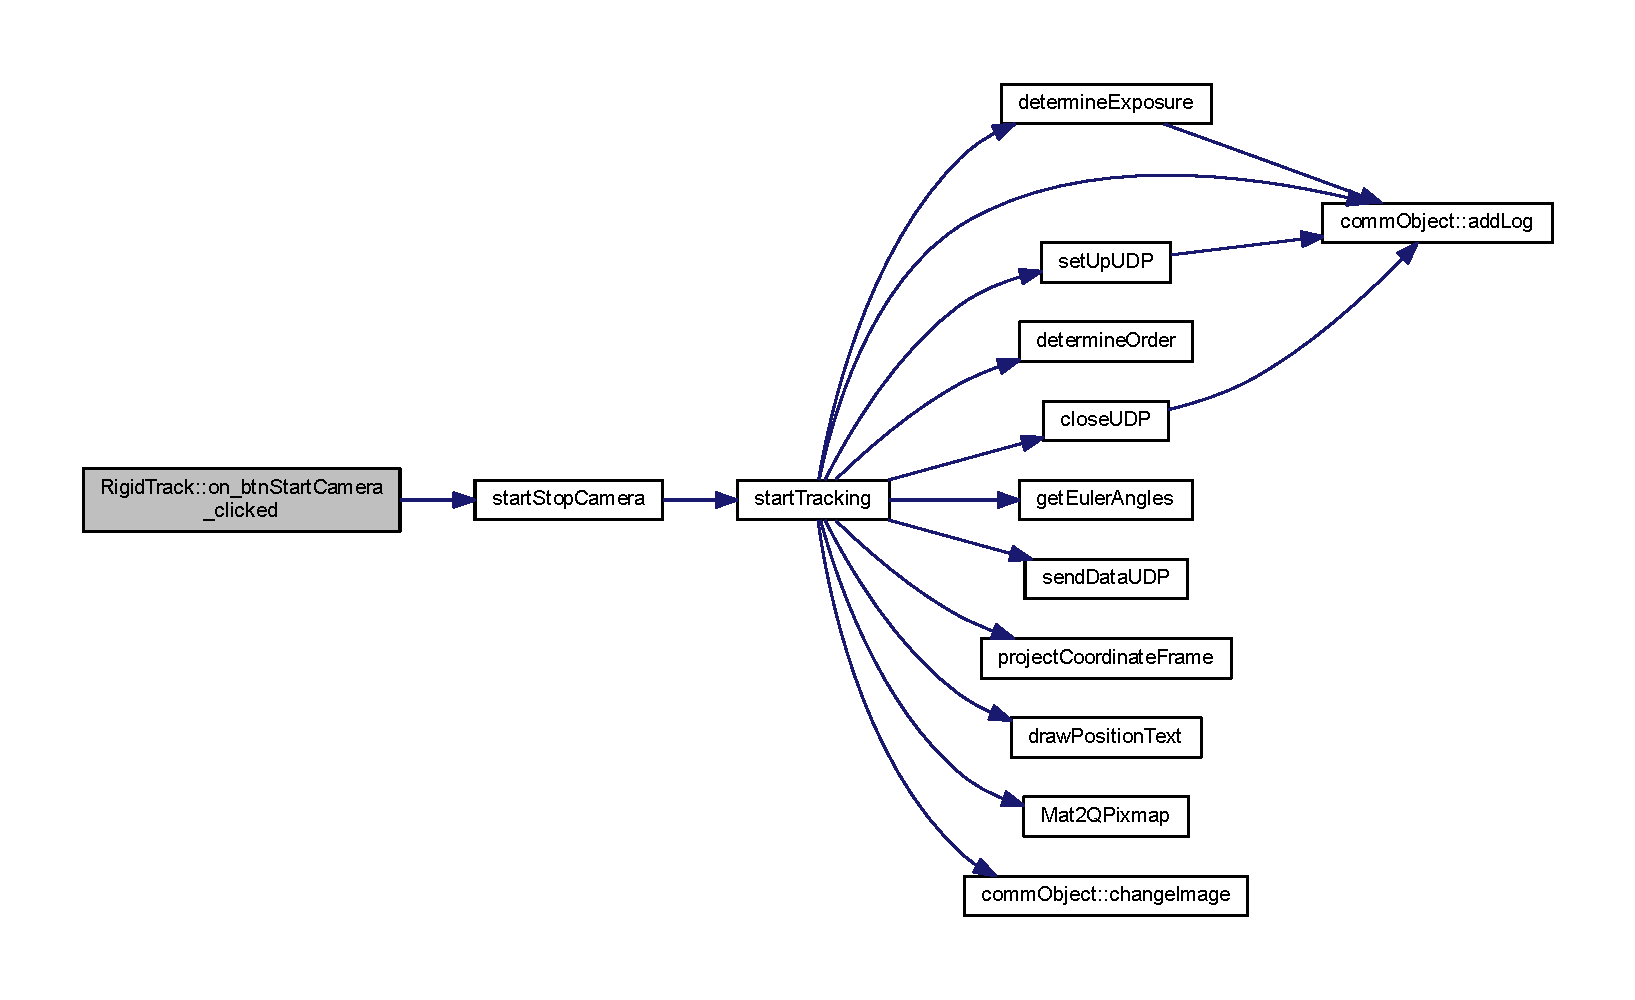
\includegraphics[width=350pt]{class_rigid_track_a2f226856e28868c8bb1854fa16531f60_cgraph}
\end{center}
\end{figure}
\mbox{\Hypertarget{class_rigid_track_afb1a4edcacc818db4ec6bb017dd07e0f}\label{class_rigid_track_afb1a4edcacc818db4ec6bb017dd07e0f}} 
\index{Rigid\+Track@{Rigid\+Track}!on\+\_\+btn\+Zero\+\_\+clicked@{on\+\_\+btn\+Zero\+\_\+clicked}}
\index{on\+\_\+btn\+Zero\+\_\+clicked@{on\+\_\+btn\+Zero\+\_\+clicked}!Rigid\+Track@{Rigid\+Track}}
\subsubsection{\texorpdfstring{on\+\_\+btn\+Zero\+\_\+clicked}{on\_btnZero\_clicked}}
{\footnotesize\ttfamily void Rigid\+Track\+::on\+\_\+btn\+Zero\+\_\+clicked (\begin{DoxyParamCaption}{ }\end{DoxyParamCaption})\hspace{0.3cm}{\ttfamily [slot]}}

Here is the call graph for this function\+:\nopagebreak
\begin{figure}[H]
\begin{center}
\leavevmode
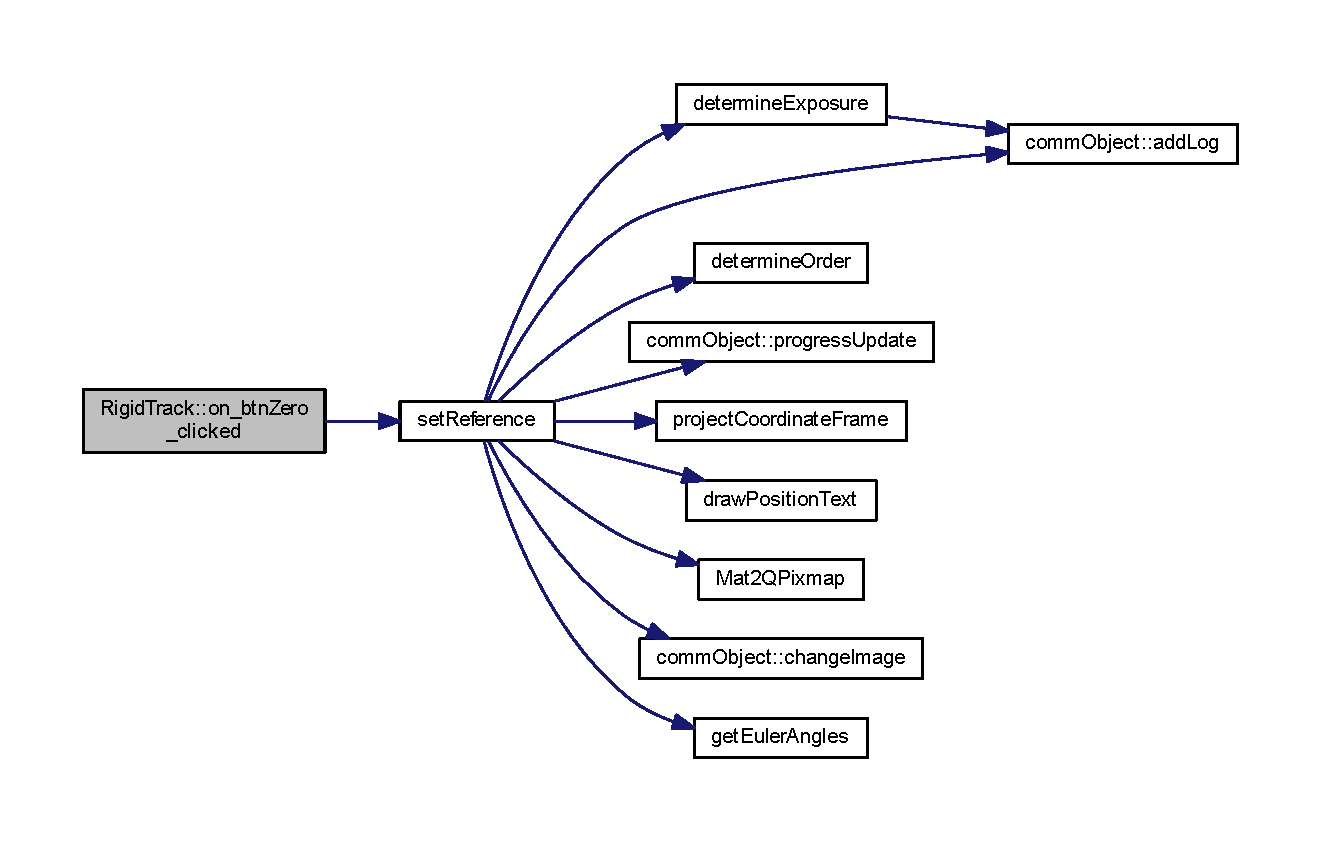
\includegraphics[width=350pt]{class_rigid_track_afb1a4edcacc818db4ec6bb017dd07e0f_cgraph}
\end{center}
\end{figure}
\mbox{\Hypertarget{class_rigid_track_ab347b3edeca55685f4d601549596d44a}\label{class_rigid_track_ab347b3edeca55685f4d601549596d44a}} 
\index{Rigid\+Track@{Rigid\+Track}!on\+\_\+cb\+Invert\+\_\+state\+Changed@{on\+\_\+cb\+Invert\+\_\+state\+Changed}}
\index{on\+\_\+cb\+Invert\+\_\+state\+Changed@{on\+\_\+cb\+Invert\+\_\+state\+Changed}!Rigid\+Track@{Rigid\+Track}}
\subsubsection{\texorpdfstring{on\+\_\+cb\+Invert\+\_\+state\+Changed}{on\_cbInvert\_stateChanged}}
{\footnotesize\ttfamily void Rigid\+Track\+::on\+\_\+cb\+Invert\+\_\+state\+Changed (\begin{DoxyParamCaption}\item[{int}]{state }\end{DoxyParamCaption})\hspace{0.3cm}{\ttfamily [slot]}}

\mbox{\Hypertarget{class_rigid_track_ad6ba1cfe25f18ff0d9f5993aafa36d16}\label{class_rigid_track_ad6ba1cfe25f18ff0d9f5993aafa36d16}} 
\index{Rigid\+Track@{Rigid\+Track}!on\+\_\+cb\+Safety2\+\_\+state\+Changed@{on\+\_\+cb\+Safety2\+\_\+state\+Changed}}
\index{on\+\_\+cb\+Safety2\+\_\+state\+Changed@{on\+\_\+cb\+Safety2\+\_\+state\+Changed}!Rigid\+Track@{Rigid\+Track}}
\subsubsection{\texorpdfstring{on\+\_\+cb\+Safety2\+\_\+state\+Changed}{on\_cbSafety2\_stateChanged}}
{\footnotesize\ttfamily void Rigid\+Track\+::on\+\_\+cb\+Safety2\+\_\+state\+Changed (\begin{DoxyParamCaption}\item[{int}]{state }\end{DoxyParamCaption})\hspace{0.3cm}{\ttfamily [slot]}}

Here is the call graph for this function\+:\nopagebreak
\begin{figure}[H]
\begin{center}
\leavevmode
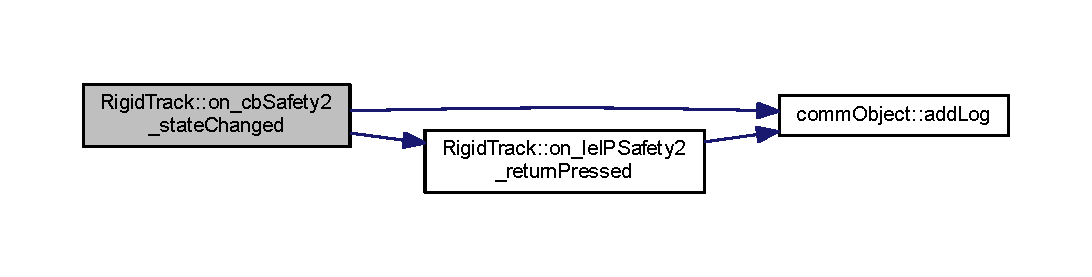
\includegraphics[width=350pt]{class_rigid_track_ad6ba1cfe25f18ff0d9f5993aafa36d16_cgraph}
\end{center}
\end{figure}
\mbox{\Hypertarget{class_rigid_track_a8f999fa968f4cc9fa548bdc8438b32c4}\label{class_rigid_track_a8f999fa968f4cc9fa548bdc8438b32c4}} 
\index{Rigid\+Track@{Rigid\+Track}!on\+\_\+cb\+Safety\+\_\+state\+Changed@{on\+\_\+cb\+Safety\+\_\+state\+Changed}}
\index{on\+\_\+cb\+Safety\+\_\+state\+Changed@{on\+\_\+cb\+Safety\+\_\+state\+Changed}!Rigid\+Track@{Rigid\+Track}}
\subsubsection{\texorpdfstring{on\+\_\+cb\+Safety\+\_\+state\+Changed}{on\_cbSafety\_stateChanged}}
{\footnotesize\ttfamily void Rigid\+Track\+::on\+\_\+cb\+Safety\+\_\+state\+Changed (\begin{DoxyParamCaption}\item[{int}]{state }\end{DoxyParamCaption})\hspace{0.3cm}{\ttfamily [slot]}}

Here is the call graph for this function\+:\nopagebreak
\begin{figure}[H]
\begin{center}
\leavevmode
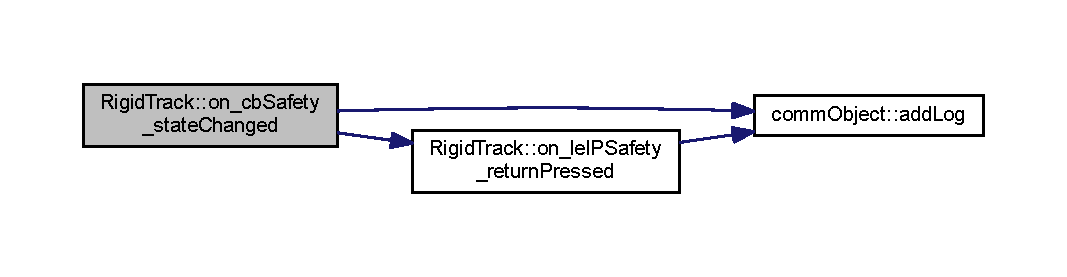
\includegraphics[width=350pt]{class_rigid_track_a8f999fa968f4cc9fa548bdc8438b32c4_cgraph}
\end{center}
\end{figure}
\mbox{\Hypertarget{class_rigid_track_ae5e44de9f4e3cacdd647c0305936b02b}\label{class_rigid_track_ae5e44de9f4e3cacdd647c0305936b02b}} 
\index{Rigid\+Track@{Rigid\+Track}!on\+\_\+dsb\+Dimension\+\_\+value\+Changed@{on\+\_\+dsb\+Dimension\+\_\+value\+Changed}}
\index{on\+\_\+dsb\+Dimension\+\_\+value\+Changed@{on\+\_\+dsb\+Dimension\+\_\+value\+Changed}!Rigid\+Track@{Rigid\+Track}}
\subsubsection{\texorpdfstring{on\+\_\+dsb\+Dimension\+\_\+value\+Changed}{on\_dsbDimension\_valueChanged}}
{\footnotesize\ttfamily void Rigid\+Track\+::on\+\_\+dsb\+Dimension\+\_\+value\+Changed (\begin{DoxyParamCaption}\item[{double}]{d }\end{DoxyParamCaption})\hspace{0.3cm}{\ttfamily [slot]}}

\mbox{\Hypertarget{class_rigid_track_a9f037a061b2577815fc80e5e9f8d46d9}\label{class_rigid_track_a9f037a061b2577815fc80e5e9f8d46d9}} 
\index{Rigid\+Track@{Rigid\+Track}!on\+\_\+le\+I\+P\+Object\+\_\+return\+Pressed@{on\+\_\+le\+I\+P\+Object\+\_\+return\+Pressed}}
\index{on\+\_\+le\+I\+P\+Object\+\_\+return\+Pressed@{on\+\_\+le\+I\+P\+Object\+\_\+return\+Pressed}!Rigid\+Track@{Rigid\+Track}}
\subsubsection{\texorpdfstring{on\+\_\+le\+I\+P\+Object\+\_\+return\+Pressed}{on\_leIPObject\_returnPressed}}
{\footnotesize\ttfamily void Rigid\+Track\+::on\+\_\+le\+I\+P\+Object\+\_\+return\+Pressed (\begin{DoxyParamCaption}{ }\end{DoxyParamCaption})\hspace{0.3cm}{\ttfamily [slot]}}

Here is the call graph for this function\+:\nopagebreak
\begin{figure}[H]
\begin{center}
\leavevmode
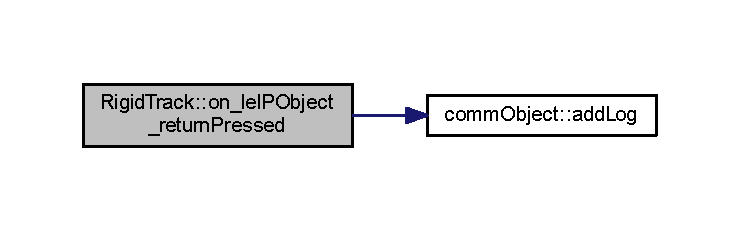
\includegraphics[width=350pt]{class_rigid_track_a9f037a061b2577815fc80e5e9f8d46d9_cgraph}
\end{center}
\end{figure}
\mbox{\Hypertarget{class_rigid_track_a555c536593d659b940de43cd2db8d6c1}\label{class_rigid_track_a555c536593d659b940de43cd2db8d6c1}} 
\index{Rigid\+Track@{Rigid\+Track}!on\+\_\+le\+I\+P\+Safety2\+\_\+return\+Pressed@{on\+\_\+le\+I\+P\+Safety2\+\_\+return\+Pressed}}
\index{on\+\_\+le\+I\+P\+Safety2\+\_\+return\+Pressed@{on\+\_\+le\+I\+P\+Safety2\+\_\+return\+Pressed}!Rigid\+Track@{Rigid\+Track}}
\subsubsection{\texorpdfstring{on\+\_\+le\+I\+P\+Safety2\+\_\+return\+Pressed}{on\_leIPSafety2\_returnPressed}}
{\footnotesize\ttfamily void Rigid\+Track\+::on\+\_\+le\+I\+P\+Safety2\+\_\+return\+Pressed (\begin{DoxyParamCaption}{ }\end{DoxyParamCaption})\hspace{0.3cm}{\ttfamily [slot]}}

Here is the call graph for this function\+:\nopagebreak
\begin{figure}[H]
\begin{center}
\leavevmode
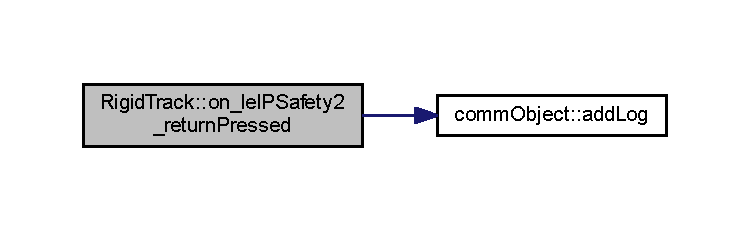
\includegraphics[width=350pt]{class_rigid_track_a555c536593d659b940de43cd2db8d6c1_cgraph}
\end{center}
\end{figure}
Here is the caller graph for this function\+:\nopagebreak
\begin{figure}[H]
\begin{center}
\leavevmode
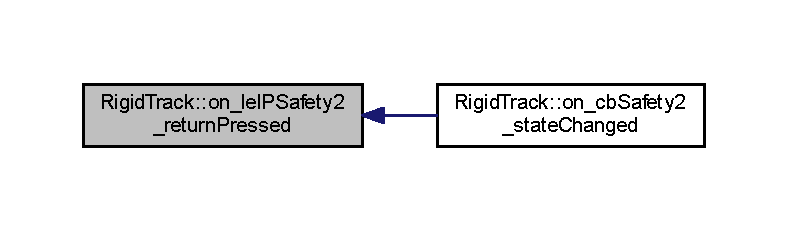
\includegraphics[width=350pt]{class_rigid_track_a555c536593d659b940de43cd2db8d6c1_icgraph}
\end{center}
\end{figure}
\mbox{\Hypertarget{class_rigid_track_aa527ab3a2ddc7b31bf1063260efc9755}\label{class_rigid_track_aa527ab3a2ddc7b31bf1063260efc9755}} 
\index{Rigid\+Track@{Rigid\+Track}!on\+\_\+le\+I\+P\+Safety\+\_\+return\+Pressed@{on\+\_\+le\+I\+P\+Safety\+\_\+return\+Pressed}}
\index{on\+\_\+le\+I\+P\+Safety\+\_\+return\+Pressed@{on\+\_\+le\+I\+P\+Safety\+\_\+return\+Pressed}!Rigid\+Track@{Rigid\+Track}}
\subsubsection{\texorpdfstring{on\+\_\+le\+I\+P\+Safety\+\_\+return\+Pressed}{on\_leIPSafety\_returnPressed}}
{\footnotesize\ttfamily void Rigid\+Track\+::on\+\_\+le\+I\+P\+Safety\+\_\+return\+Pressed (\begin{DoxyParamCaption}{ }\end{DoxyParamCaption})\hspace{0.3cm}{\ttfamily [slot]}}

Here is the call graph for this function\+:\nopagebreak
\begin{figure}[H]
\begin{center}
\leavevmode
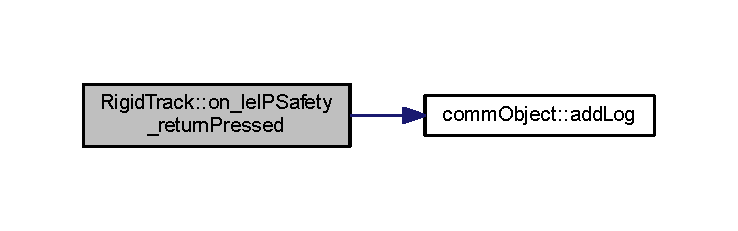
\includegraphics[width=350pt]{class_rigid_track_aa527ab3a2ddc7b31bf1063260efc9755_cgraph}
\end{center}
\end{figure}
Here is the caller graph for this function\+:\nopagebreak
\begin{figure}[H]
\begin{center}
\leavevmode
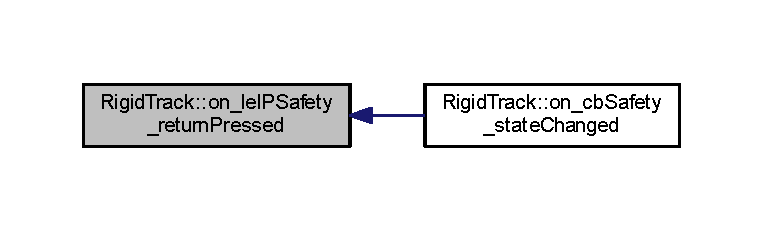
\includegraphics[width=350pt]{class_rigid_track_aa527ab3a2ddc7b31bf1063260efc9755_icgraph}
\end{center}
\end{figure}
\mbox{\Hypertarget{class_rigid_track_ad3e07592fbc1491cdc36dd5e817e1775}\label{class_rigid_track_ad3e07592fbc1491cdc36dd5e817e1775}} 
\index{Rigid\+Track@{Rigid\+Track}!on\+\_\+pb\+Load\+Marker\+\_\+clicked@{on\+\_\+pb\+Load\+Marker\+\_\+clicked}}
\index{on\+\_\+pb\+Load\+Marker\+\_\+clicked@{on\+\_\+pb\+Load\+Marker\+\_\+clicked}!Rigid\+Track@{Rigid\+Track}}
\subsubsection{\texorpdfstring{on\+\_\+pb\+Load\+Marker\+\_\+clicked}{on\_pbLoadMarker\_clicked}}
{\footnotesize\ttfamily void Rigid\+Track\+::on\+\_\+pb\+Load\+Marker\+\_\+clicked (\begin{DoxyParamCaption}{ }\end{DoxyParamCaption})\hspace{0.3cm}{\ttfamily [slot]}}

Here is the call graph for this function\+:\nopagebreak
\begin{figure}[H]
\begin{center}
\leavevmode
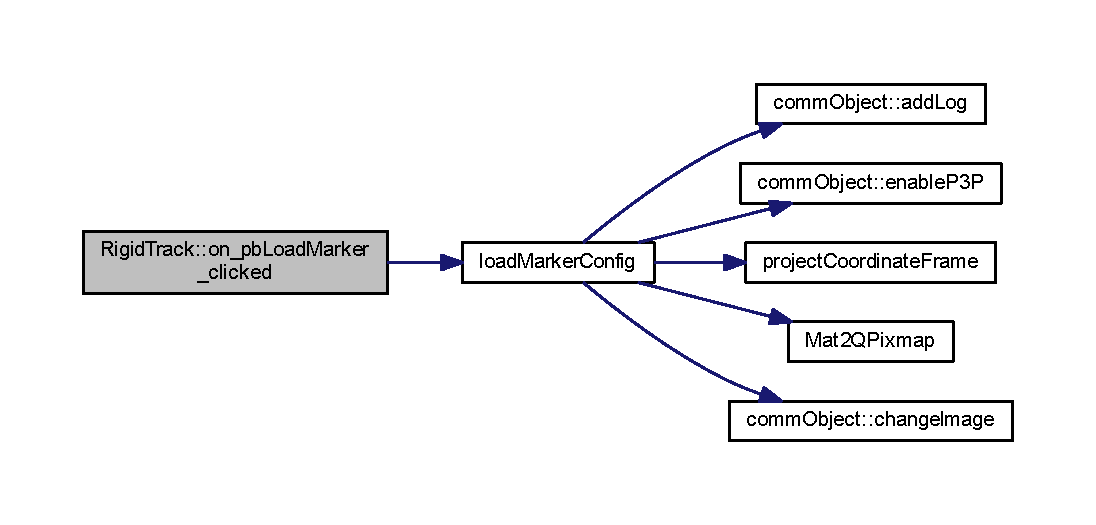
\includegraphics[width=350pt]{class_rigid_track_ad3e07592fbc1491cdc36dd5e817e1775_cgraph}
\end{center}
\end{figure}
\mbox{\Hypertarget{class_rigid_track_a19bc46333f946e589184eeed998160da}\label{class_rigid_track_a19bc46333f946e589184eeed998160da}} 
\index{Rigid\+Track@{Rigid\+Track}!on\+\_\+rb\+E\+Pn\+P\+\_\+clicked@{on\+\_\+rb\+E\+Pn\+P\+\_\+clicked}}
\index{on\+\_\+rb\+E\+Pn\+P\+\_\+clicked@{on\+\_\+rb\+E\+Pn\+P\+\_\+clicked}!Rigid\+Track@{Rigid\+Track}}
\subsubsection{\texorpdfstring{on\+\_\+rb\+E\+Pn\+P\+\_\+clicked}{on\_rbEPnP\_clicked}}
{\footnotesize\ttfamily void Rigid\+Track\+::on\+\_\+rb\+E\+Pn\+P\+\_\+clicked (\begin{DoxyParamCaption}{ }\end{DoxyParamCaption})\hspace{0.3cm}{\ttfamily [slot]}}

Here is the call graph for this function\+:\nopagebreak
\begin{figure}[H]
\begin{center}
\leavevmode
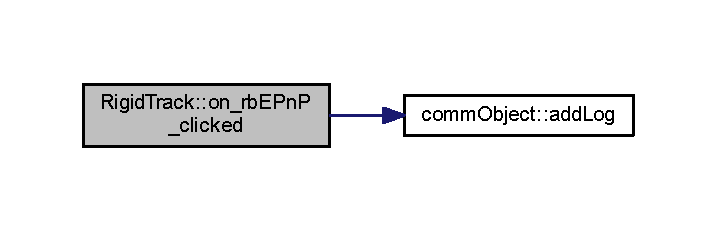
\includegraphics[width=344pt]{class_rigid_track_a19bc46333f946e589184eeed998160da_cgraph}
\end{center}
\end{figure}
\mbox{\Hypertarget{class_rigid_track_ae5bcdd3fb7203b4a7d1fa97c1460af31}\label{class_rigid_track_ae5bcdd3fb7203b4a7d1fa97c1460af31}} 
\index{Rigid\+Track@{Rigid\+Track}!on\+\_\+rb\+Iterative\+\_\+clicked@{on\+\_\+rb\+Iterative\+\_\+clicked}}
\index{on\+\_\+rb\+Iterative\+\_\+clicked@{on\+\_\+rb\+Iterative\+\_\+clicked}!Rigid\+Track@{Rigid\+Track}}
\subsubsection{\texorpdfstring{on\+\_\+rb\+Iterative\+\_\+clicked}{on\_rbIterative\_clicked}}
{\footnotesize\ttfamily void Rigid\+Track\+::on\+\_\+rb\+Iterative\+\_\+clicked (\begin{DoxyParamCaption}{ }\end{DoxyParamCaption})\hspace{0.3cm}{\ttfamily [slot]}}

Here is the call graph for this function\+:\nopagebreak
\begin{figure}[H]
\begin{center}
\leavevmode
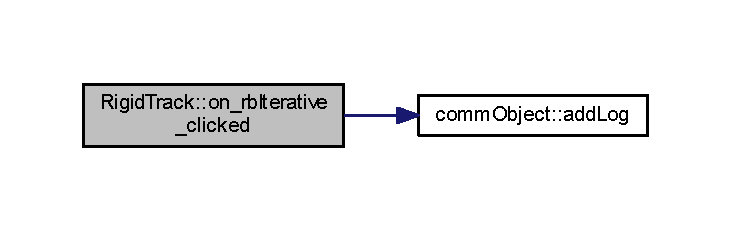
\includegraphics[width=350pt]{class_rigid_track_ae5bcdd3fb7203b4a7d1fa97c1460af31_cgraph}
\end{center}
\end{figure}
\mbox{\Hypertarget{class_rigid_track_ac1f10ea5ec3f718c152e245a04776454}\label{class_rigid_track_ac1f10ea5ec3f718c152e245a04776454}} 
\index{Rigid\+Track@{Rigid\+Track}!on\+\_\+rb\+P3\+P\+\_\+clicked@{on\+\_\+rb\+P3\+P\+\_\+clicked}}
\index{on\+\_\+rb\+P3\+P\+\_\+clicked@{on\+\_\+rb\+P3\+P\+\_\+clicked}!Rigid\+Track@{Rigid\+Track}}
\subsubsection{\texorpdfstring{on\+\_\+rb\+P3\+P\+\_\+clicked}{on\_rbP3P\_clicked}}
{\footnotesize\ttfamily void Rigid\+Track\+::on\+\_\+rb\+P3\+P\+\_\+clicked (\begin{DoxyParamCaption}{ }\end{DoxyParamCaption})\hspace{0.3cm}{\ttfamily [slot]}}

Here is the call graph for this function\+:\nopagebreak
\begin{figure}[H]
\begin{center}
\leavevmode
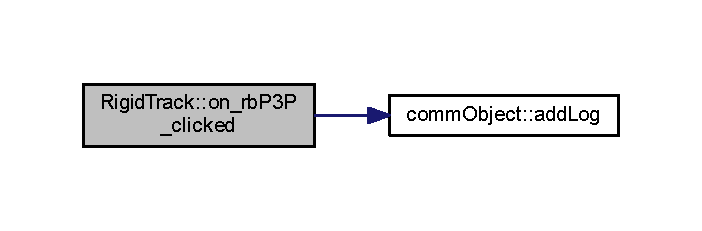
\includegraphics[width=337pt]{class_rigid_track_ac1f10ea5ec3f718c152e245a04776454_cgraph}
\end{center}
\end{figure}
\mbox{\Hypertarget{class_rigid_track_a217ca3d828c99943ea155e6891264b24}\label{class_rigid_track_a217ca3d828c99943ea155e6891264b24}} 
\index{Rigid\+Track@{Rigid\+Track}!on\+\_\+sb\+Angle\+\_\+value\+Changed@{on\+\_\+sb\+Angle\+\_\+value\+Changed}}
\index{on\+\_\+sb\+Angle\+\_\+value\+Changed@{on\+\_\+sb\+Angle\+\_\+value\+Changed}!Rigid\+Track@{Rigid\+Track}}
\subsubsection{\texorpdfstring{on\+\_\+sb\+Angle\+\_\+value\+Changed}{on\_sbAngle\_valueChanged}}
{\footnotesize\ttfamily void Rigid\+Track\+::on\+\_\+sb\+Angle\+\_\+value\+Changed (\begin{DoxyParamCaption}\item[{int}]{i }\end{DoxyParamCaption})\hspace{0.3cm}{\ttfamily [slot]}}

\mbox{\Hypertarget{class_rigid_track_a72e338d6bf93d0efa3bc503f7ca736c5}\label{class_rigid_track_a72e338d6bf93d0efa3bc503f7ca736c5}} 
\index{Rigid\+Track@{Rigid\+Track}!on\+\_\+sb\+Heading\+Offset\+\_\+value\+Changed@{on\+\_\+sb\+Heading\+Offset\+\_\+value\+Changed}}
\index{on\+\_\+sb\+Heading\+Offset\+\_\+value\+Changed@{on\+\_\+sb\+Heading\+Offset\+\_\+value\+Changed}!Rigid\+Track@{Rigid\+Track}}
\subsubsection{\texorpdfstring{on\+\_\+sb\+Heading\+Offset\+\_\+value\+Changed}{on\_sbHeadingOffset\_valueChanged}}
{\footnotesize\ttfamily void Rigid\+Track\+::on\+\_\+sb\+Heading\+Offset\+\_\+value\+Changed (\begin{DoxyParamCaption}\item[{double}]{d }\end{DoxyParamCaption})\hspace{0.3cm}{\ttfamily [slot]}}

Here is the call graph for this function\+:\nopagebreak
\begin{figure}[H]
\begin{center}
\leavevmode
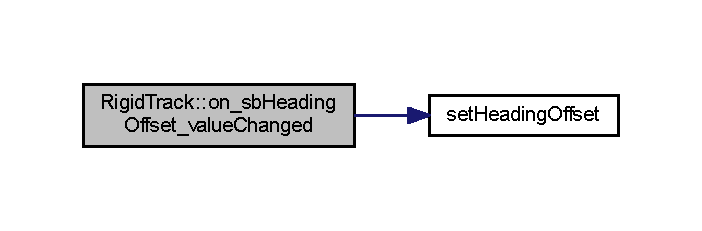
\includegraphics[width=337pt]{class_rigid_track_a72e338d6bf93d0efa3bc503f7ca736c5_cgraph}
\end{center}
\end{figure}
\mbox{\Hypertarget{class_rigid_track_a9d229d23fdf40b988a1743accb695ea8}\label{class_rigid_track_a9d229d23fdf40b988a1743accb695ea8}} 
\index{Rigid\+Track@{Rigid\+Track}!progress\+Update@{progress\+Update}}
\index{progress\+Update@{progress\+Update}!Rigid\+Track@{Rigid\+Track}}
\subsubsection{\texorpdfstring{progress\+Update}{progressUpdate}}
{\footnotesize\ttfamily void Rigid\+Track\+::progress\+Update (\begin{DoxyParamCaption}\item[{int}]{value }\end{DoxyParamCaption})\hspace{0.3cm}{\ttfamily [slot]}}

\mbox{\Hypertarget{class_rigid_track_a3b0b3835204cad40abdb144d24aefc76}\label{class_rigid_track_a3b0b3835204cad40abdb144d24aefc76}} 
\index{Rigid\+Track@{Rigid\+Track}!set\+Image@{set\+Image}}
\index{set\+Image@{set\+Image}!Rigid\+Track@{Rigid\+Track}}
\subsubsection{\texorpdfstring{set\+Image}{setImage}}
{\footnotesize\ttfamily void Rigid\+Track\+::set\+Image (\begin{DoxyParamCaption}\item[{Q\+Pixmap}]{image }\end{DoxyParamCaption})\hspace{0.3cm}{\ttfamily [slot]}}

\mbox{\Hypertarget{class_rigid_track_a54a029af74a21f92749e99df7ed847b2}\label{class_rigid_track_a54a029af74a21f92749e99df7ed847b2}} 
\index{Rigid\+Track@{Rigid\+Track}!set\+Log@{set\+Log}}
\index{set\+Log@{set\+Log}!Rigid\+Track@{Rigid\+Track}}
\subsubsection{\texorpdfstring{set\+Log}{setLog}}
{\footnotesize\ttfamily void Rigid\+Track\+::set\+Log (\begin{DoxyParamCaption}\item[{Q\+String}]{log\+Text }\end{DoxyParamCaption})\hspace{0.3cm}{\ttfamily [slot]}}



The documentation for this class was generated from the following files\+:\begin{DoxyCompactItemize}
\item 
Rigid\+Track/\hyperlink{_rigid_track_8h}{Rigid\+Track.\+h}\item 
Rigid\+Track/\hyperlink{_rigid_track_8cpp}{Rigid\+Track.\+cpp}\end{DoxyCompactItemize}

\hypertarget{class_ui_1_1_rigid_track_class}{}\section{Ui\+:\+:Rigid\+Track\+Class Class Reference}
\label{class_ui_1_1_rigid_track_class}\index{Ui\+::\+Rigid\+Track\+Class@{Ui\+::\+Rigid\+Track\+Class}}


{\ttfamily \#include $<$ui\+\_\+\+Rigid\+Track.\+h$>$}



Inheritance diagram for Ui\+:\+:Rigid\+Track\+Class\+:\nopagebreak
\begin{figure}[H]
\begin{center}
\leavevmode
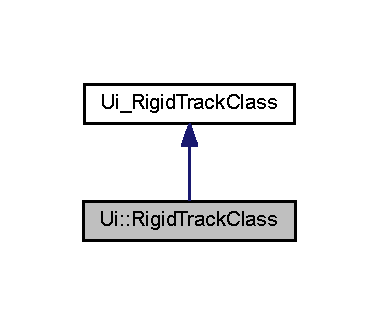
\includegraphics[width=182pt]{class_ui_1_1_rigid_track_class__inherit__graph}
\end{center}
\end{figure}


Collaboration diagram for Ui\+:\+:Rigid\+Track\+Class\+:\nopagebreak
\begin{figure}[H]
\begin{center}
\leavevmode
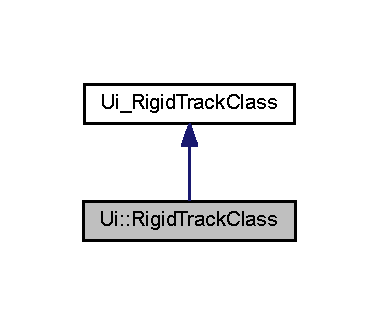
\includegraphics[width=182pt]{class_ui_1_1_rigid_track_class__coll__graph}
\end{center}
\end{figure}
\subsection*{Additional Inherited Members}


\subsection{Detailed Description}


Definition at line 304 of file ui\+\_\+\+Rigid\+Track.\+h.



The documentation for this class was generated from the following file\+:\begin{DoxyCompactItemize}
\item 
Rigid\+Track/\+Generated\+Files/\hyperlink{ui___rigid_track_8h}{ui\+\_\+\+Rigid\+Track.\+h}\end{DoxyCompactItemize}

\hypertarget{class_surface}{}\section{Surface Class Reference}
\label{class_surface}\index{Surface@{Surface}}


{\ttfamily \#include $<$supportcode.\+h$>$}

\subsection*{Public Member Functions}
\begin{DoxyCompactItemize}
\item 
\hyperlink{class_surface_a323ba9165c8635e84eb0c490fe88d846}{Surface} (int \hyperlink{class_surface_ae76d7c2fa208df6979a77cc60e8105c0}{Width}, int \hyperlink{class_surface_ab901f48d51b3fd427415b580dc15518c}{Height})
\begin{DoxyCompactList}\small\item\em /$<$============================== \end{DoxyCompactList}\item 
\hyperlink{class_surface_a89de75c95cb550d432f3ea4ed1429db0}{$\sim$\+Surface} ()
\item 
G\+Luint \hyperlink{class_surface_a2cd8789d26457187b8af4be8c178e9d4}{Get\+Texture} ()
\item 
void \hyperlink{class_surface_a5e45e936e3057fa1ddad0c7924767005}{Resize} (int \hyperlink{class_surface_ae76d7c2fa208df6979a77cc60e8105c0}{Width}, int \hyperlink{class_surface_ab901f48d51b3fd427415b580dc15518c}{Height})
\item 
int \hyperlink{class_surface_aeb8a8540f415a4d29c440667e8532e91}{Calculate\+Size} (int \hyperlink{class_surface_ae76d7c2fa208df6979a77cc60e8105c0}{Width})
\item 
int \hyperlink{class_surface_ae76d7c2fa208df6979a77cc60e8105c0}{Width} ()
\item 
int \hyperlink{class_surface_ab901f48d51b3fd427415b580dc15518c}{Height} ()
\item 
int \hyperlink{class_surface_a4cbf23ea0c8ff533271109fc2a1a863d}{Surface\+Width} ()
\item 
int \hyperlink{class_surface_a377c59f6ef131d4b879cda93578a3efa}{Surface\+Height} ()
\item 
void \hyperlink{class_surface_a728571d0386e9690ce1760931562c72b}{Put\+Pixel} (int X, int Y, P\+I\+X\+EL Color)
\item 
unsigned char $\ast$ \hyperlink{class_surface_a8f8da8f3ee82b8e657916f40b3f40eff}{Get\+Buffer} ()
\item 
void \hyperlink{class_surface_aa75c49f53fec5c49ba8422c0d64815e6}{Rebind\+Texture} ()
\item 
int \hyperlink{class_surface_abe0d542404575c60911d6ad4219560f9}{Pixel\+Span} ()
\end{DoxyCompactItemize}


\subsection{Constructor \& Destructor Documentation}
\mbox{\Hypertarget{class_surface_a323ba9165c8635e84eb0c490fe88d846}\label{class_surface_a323ba9165c8635e84eb0c490fe88d846}} 
\index{Surface@{Surface}!Surface@{Surface}}
\index{Surface@{Surface}!Surface@{Surface}}
\subsubsection{\texorpdfstring{Surface()}{Surface()}}
{\footnotesize\ttfamily Surface\+::\+Surface (\begin{DoxyParamCaption}\item[{int}]{Width,  }\item[{int}]{Height }\end{DoxyParamCaption})}



/$<$============================== 

/$<$== Use power of 2 texture sizes == Here is the call graph for this function\+:
\nopagebreak
\begin{figure}[H]
\begin{center}
\leavevmode
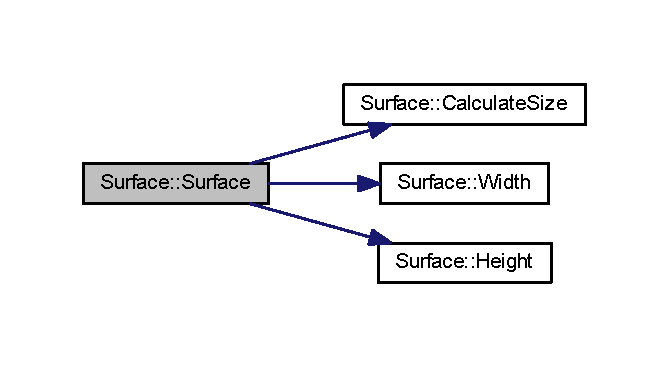
\includegraphics[width=321pt]{class_surface_a323ba9165c8635e84eb0c490fe88d846_cgraph}
\end{center}
\end{figure}
\mbox{\Hypertarget{class_surface_a89de75c95cb550d432f3ea4ed1429db0}\label{class_surface_a89de75c95cb550d432f3ea4ed1429db0}} 
\index{Surface@{Surface}!````~Surface@{$\sim$\+Surface}}
\index{````~Surface@{$\sim$\+Surface}!Surface@{Surface}}
\subsubsection{\texorpdfstring{$\sim$\+Surface()}{~Surface()}}
{\footnotesize\ttfamily Surface\+::$\sim$\+Surface (\begin{DoxyParamCaption}{ }\end{DoxyParamCaption})}



\subsection{Member Function Documentation}
\mbox{\Hypertarget{class_surface_aeb8a8540f415a4d29c440667e8532e91}\label{class_surface_aeb8a8540f415a4d29c440667e8532e91}} 
\index{Surface@{Surface}!Calculate\+Size@{Calculate\+Size}}
\index{Calculate\+Size@{Calculate\+Size}!Surface@{Surface}}
\subsubsection{\texorpdfstring{Calculate\+Size()}{CalculateSize()}}
{\footnotesize\ttfamily int Surface\+::\+Calculate\+Size (\begin{DoxyParamCaption}\item[{int}]{Width }\end{DoxyParamCaption})}

Here is the caller graph for this function\+:
\nopagebreak
\begin{figure}[H]
\begin{center}
\leavevmode
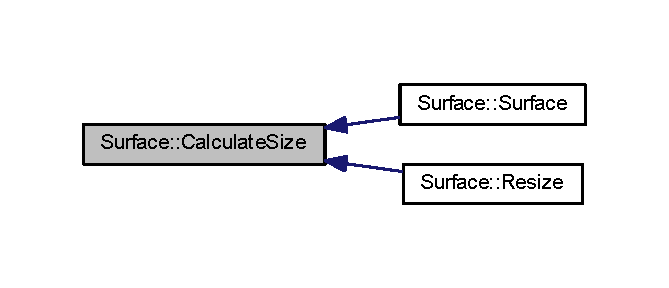
\includegraphics[width=321pt]{class_surface_aeb8a8540f415a4d29c440667e8532e91_icgraph}
\end{center}
\end{figure}
\mbox{\Hypertarget{class_surface_a8f8da8f3ee82b8e657916f40b3f40eff}\label{class_surface_a8f8da8f3ee82b8e657916f40b3f40eff}} 
\index{Surface@{Surface}!Get\+Buffer@{Get\+Buffer}}
\index{Get\+Buffer@{Get\+Buffer}!Surface@{Surface}}
\subsubsection{\texorpdfstring{Get\+Buffer()}{GetBuffer()}}
{\footnotesize\ttfamily unsigned char$\ast$ Surface\+::\+Get\+Buffer (\begin{DoxyParamCaption}{ }\end{DoxyParamCaption})\hspace{0.3cm}{\ttfamily [inline]}}

Here is the call graph for this function\+:
\nopagebreak
\begin{figure}[H]
\begin{center}
\leavevmode
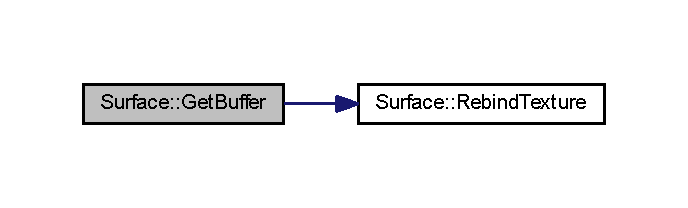
\includegraphics[width=330pt]{class_surface_a8f8da8f3ee82b8e657916f40b3f40eff_cgraph}
\end{center}
\end{figure}
\mbox{\Hypertarget{class_surface_a2cd8789d26457187b8af4be8c178e9d4}\label{class_surface_a2cd8789d26457187b8af4be8c178e9d4}} 
\index{Surface@{Surface}!Get\+Texture@{Get\+Texture}}
\index{Get\+Texture@{Get\+Texture}!Surface@{Surface}}
\subsubsection{\texorpdfstring{Get\+Texture()}{GetTexture()}}
{\footnotesize\ttfamily G\+Luint Surface\+::\+Get\+Texture (\begin{DoxyParamCaption}{ }\end{DoxyParamCaption})}

/$<$if(m\+Dirty==true) Here is the caller graph for this function\+:
\nopagebreak
\begin{figure}[H]
\begin{center}
\leavevmode
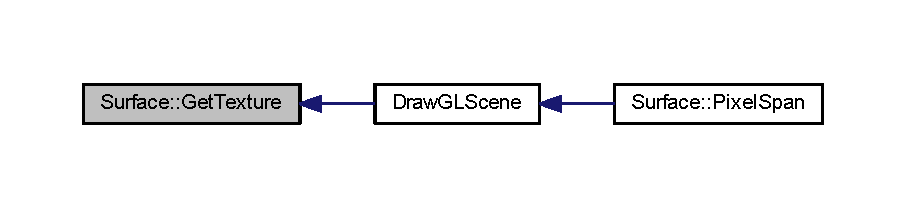
\includegraphics[width=350pt]{class_surface_a2cd8789d26457187b8af4be8c178e9d4_icgraph}
\end{center}
\end{figure}
\mbox{\Hypertarget{class_surface_ab901f48d51b3fd427415b580dc15518c}\label{class_surface_ab901f48d51b3fd427415b580dc15518c}} 
\index{Surface@{Surface}!Height@{Height}}
\index{Height@{Height}!Surface@{Surface}}
\subsubsection{\texorpdfstring{Height()}{Height()}}
{\footnotesize\ttfamily int Surface\+::\+Height (\begin{DoxyParamCaption}{ }\end{DoxyParamCaption})\hspace{0.3cm}{\ttfamily [inline]}}

Here is the caller graph for this function\+:
\nopagebreak
\begin{figure}[H]
\begin{center}
\leavevmode
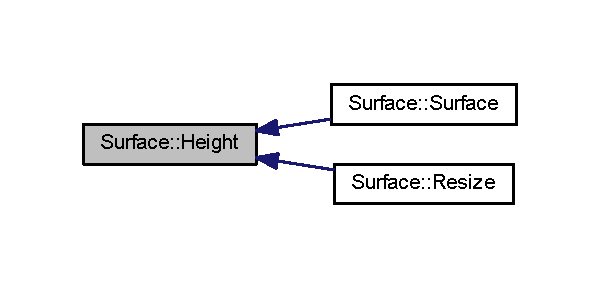
\includegraphics[width=288pt]{class_surface_ab901f48d51b3fd427415b580dc15518c_icgraph}
\end{center}
\end{figure}
\mbox{\Hypertarget{class_surface_abe0d542404575c60911d6ad4219560f9}\label{class_surface_abe0d542404575c60911d6ad4219560f9}} 
\index{Surface@{Surface}!Pixel\+Span@{Pixel\+Span}}
\index{Pixel\+Span@{Pixel\+Span}!Surface@{Surface}}
\subsubsection{\texorpdfstring{Pixel\+Span()}{PixelSpan()}}
{\footnotesize\ttfamily int Surface\+::\+Pixel\+Span (\begin{DoxyParamCaption}{ }\end{DoxyParamCaption})\hspace{0.3cm}{\ttfamily [inline]}}

Here is the call graph for this function\+:
\nopagebreak
\begin{figure}[H]
\begin{center}
\leavevmode
\includegraphics[width=350pt]{class_surface_abe0d542404575c60911d6ad4219560f9_cgraph}
\end{center}
\end{figure}
\mbox{\Hypertarget{class_surface_a728571d0386e9690ce1760931562c72b}\label{class_surface_a728571d0386e9690ce1760931562c72b}} 
\index{Surface@{Surface}!Put\+Pixel@{Put\+Pixel}}
\index{Put\+Pixel@{Put\+Pixel}!Surface@{Surface}}
\subsubsection{\texorpdfstring{Put\+Pixel()}{PutPixel()}}
{\footnotesize\ttfamily void Surface\+::\+Put\+Pixel (\begin{DoxyParamCaption}\item[{int}]{X,  }\item[{int}]{Y,  }\item[{P\+I\+X\+EL}]{Color }\end{DoxyParamCaption})}

Here is the call graph for this function\+:
\nopagebreak
\begin{figure}[H]
\begin{center}
\leavevmode
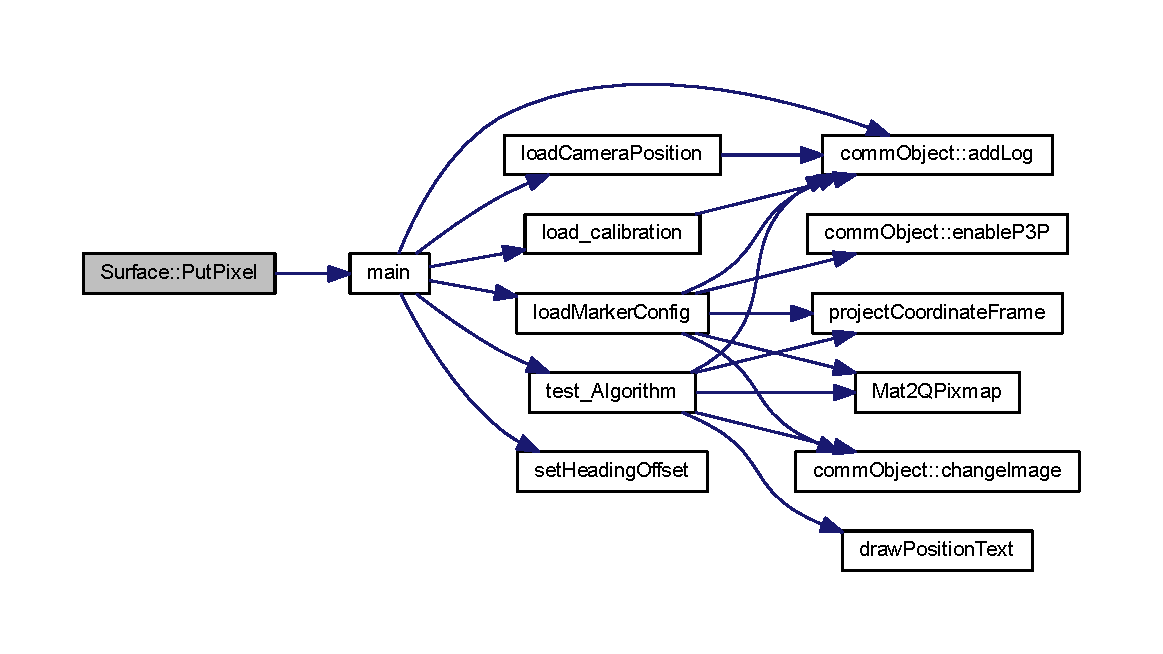
\includegraphics[width=350pt]{class_surface_a728571d0386e9690ce1760931562c72b_cgraph}
\end{center}
\end{figure}
Here is the caller graph for this function\+:
\nopagebreak
\begin{figure}[H]
\begin{center}
\leavevmode
\includegraphics[width=350pt]{class_surface_a728571d0386e9690ce1760931562c72b_icgraph}
\end{center}
\end{figure}
\mbox{\Hypertarget{class_surface_aa75c49f53fec5c49ba8422c0d64815e6}\label{class_surface_aa75c49f53fec5c49ba8422c0d64815e6}} 
\index{Surface@{Surface}!Rebind\+Texture@{Rebind\+Texture}}
\index{Rebind\+Texture@{Rebind\+Texture}!Surface@{Surface}}
\subsubsection{\texorpdfstring{Rebind\+Texture()}{RebindTexture()}}
{\footnotesize\ttfamily void Surface\+::\+Rebind\+Texture (\begin{DoxyParamCaption}{ }\end{DoxyParamCaption})}

Here is the caller graph for this function\+:
\nopagebreak
\begin{figure}[H]
\begin{center}
\leavevmode
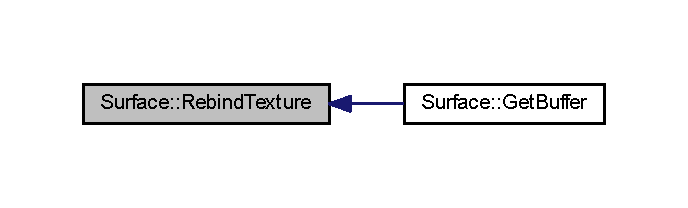
\includegraphics[width=330pt]{class_surface_aa75c49f53fec5c49ba8422c0d64815e6_icgraph}
\end{center}
\end{figure}
\mbox{\Hypertarget{class_surface_a5e45e936e3057fa1ddad0c7924767005}\label{class_surface_a5e45e936e3057fa1ddad0c7924767005}} 
\index{Surface@{Surface}!Resize@{Resize}}
\index{Resize@{Resize}!Surface@{Surface}}
\subsubsection{\texorpdfstring{Resize()}{Resize()}}
{\footnotesize\ttfamily void Surface\+::\+Resize (\begin{DoxyParamCaption}\item[{int}]{Width,  }\item[{int}]{Height }\end{DoxyParamCaption})}

Here is the call graph for this function\+:
\nopagebreak
\begin{figure}[H]
\begin{center}
\leavevmode
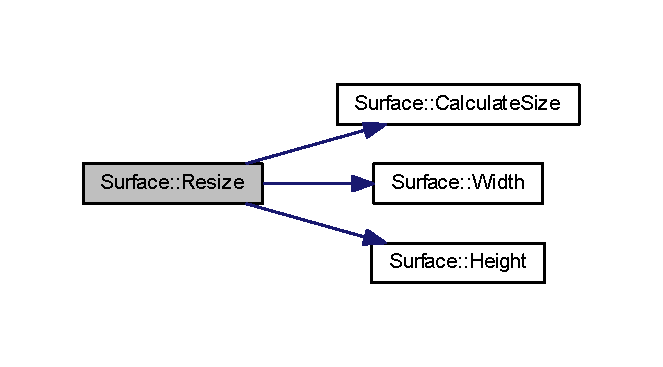
\includegraphics[width=318pt]{class_surface_a5e45e936e3057fa1ddad0c7924767005_cgraph}
\end{center}
\end{figure}
\mbox{\Hypertarget{class_surface_a377c59f6ef131d4b879cda93578a3efa}\label{class_surface_a377c59f6ef131d4b879cda93578a3efa}} 
\index{Surface@{Surface}!Surface\+Height@{Surface\+Height}}
\index{Surface\+Height@{Surface\+Height}!Surface@{Surface}}
\subsubsection{\texorpdfstring{Surface\+Height()}{SurfaceHeight()}}
{\footnotesize\ttfamily int Surface\+::\+Surface\+Height (\begin{DoxyParamCaption}{ }\end{DoxyParamCaption})\hspace{0.3cm}{\ttfamily [inline]}}

Here is the call graph for this function\+:
\nopagebreak
\begin{figure}[H]
\begin{center}
\leavevmode
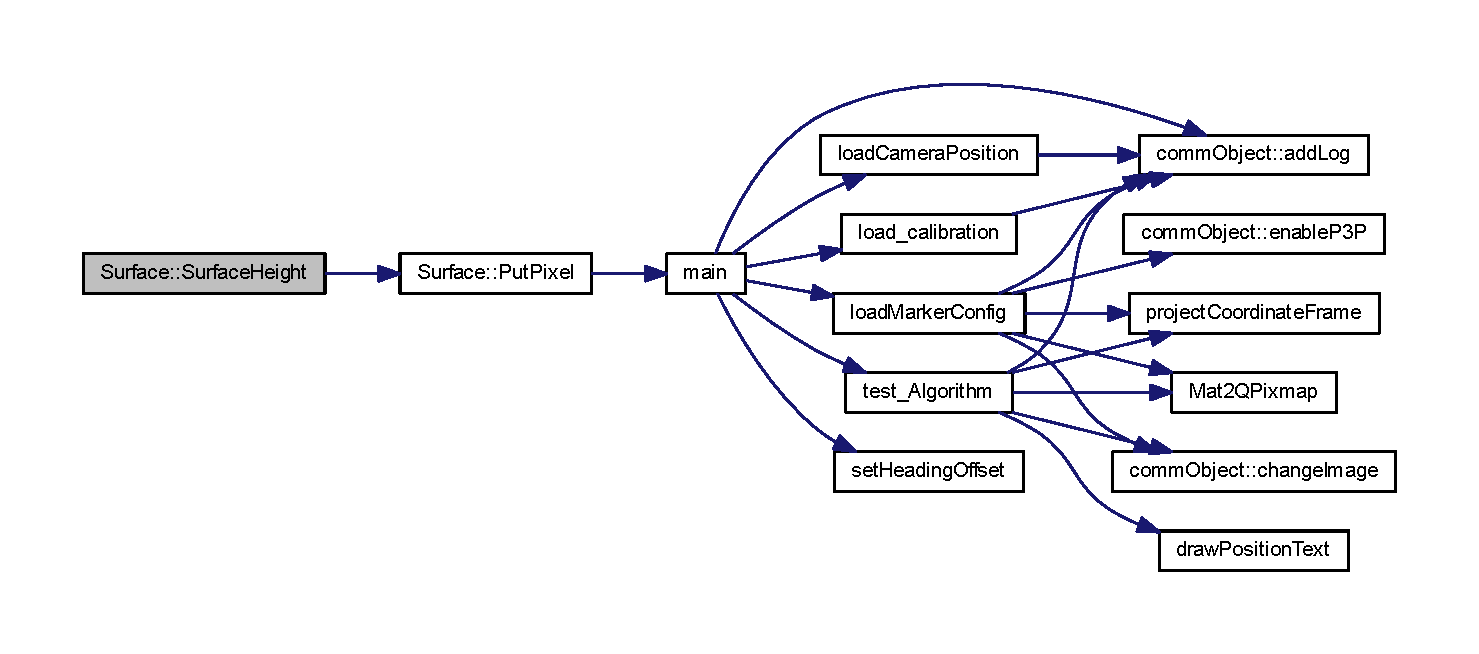
\includegraphics[width=350pt]{class_surface_a377c59f6ef131d4b879cda93578a3efa_cgraph}
\end{center}
\end{figure}
Here is the caller graph for this function\+:
\nopagebreak
\begin{figure}[H]
\begin{center}
\leavevmode
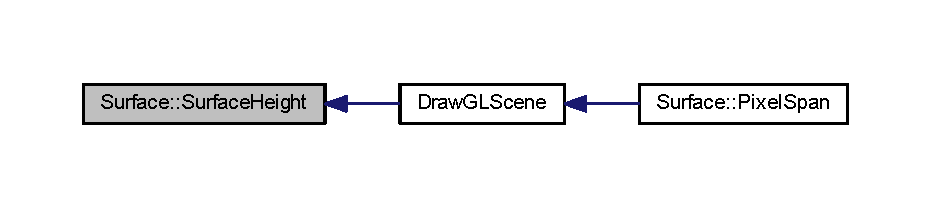
\includegraphics[width=350pt]{class_surface_a377c59f6ef131d4b879cda93578a3efa_icgraph}
\end{center}
\end{figure}
\mbox{\Hypertarget{class_surface_a4cbf23ea0c8ff533271109fc2a1a863d}\label{class_surface_a4cbf23ea0c8ff533271109fc2a1a863d}} 
\index{Surface@{Surface}!Surface\+Width@{Surface\+Width}}
\index{Surface\+Width@{Surface\+Width}!Surface@{Surface}}
\subsubsection{\texorpdfstring{Surface\+Width()}{SurfaceWidth()}}
{\footnotesize\ttfamily int Surface\+::\+Surface\+Width (\begin{DoxyParamCaption}{ }\end{DoxyParamCaption})\hspace{0.3cm}{\ttfamily [inline]}}

Here is the caller graph for this function\+:
\nopagebreak
\begin{figure}[H]
\begin{center}
\leavevmode
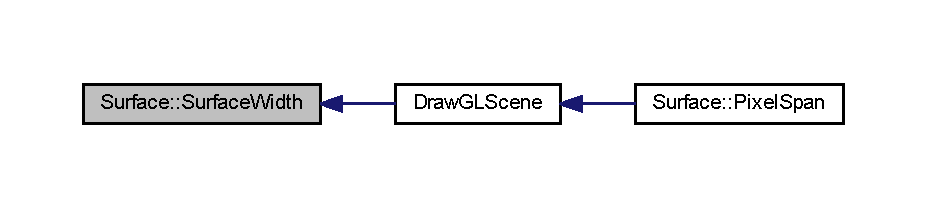
\includegraphics[width=350pt]{class_surface_a4cbf23ea0c8ff533271109fc2a1a863d_icgraph}
\end{center}
\end{figure}
\mbox{\Hypertarget{class_surface_ae76d7c2fa208df6979a77cc60e8105c0}\label{class_surface_ae76d7c2fa208df6979a77cc60e8105c0}} 
\index{Surface@{Surface}!Width@{Width}}
\index{Width@{Width}!Surface@{Surface}}
\subsubsection{\texorpdfstring{Width()}{Width()}}
{\footnotesize\ttfamily int Surface\+::\+Width (\begin{DoxyParamCaption}{ }\end{DoxyParamCaption})\hspace{0.3cm}{\ttfamily [inline]}}

Here is the caller graph for this function\+:
\nopagebreak
\begin{figure}[H]
\begin{center}
\leavevmode
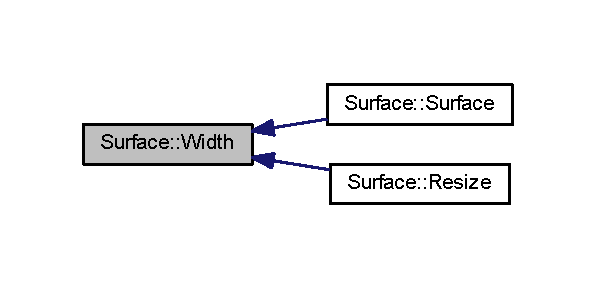
\includegraphics[width=286pt]{class_surface_ae76d7c2fa208df6979a77cc60e8105c0_icgraph}
\end{center}
\end{figure}


The documentation for this class was generated from the following files\+:\begin{DoxyCompactItemize}
\item 
Rigid\+Track/\hyperlink{supportcode_8h}{supportcode.\+h}\item 
Rigid\+Track/\hyperlink{supportcode_8cpp}{supportcode.\+cpp}\end{DoxyCompactItemize}

\hypertarget{class_ui___rigid_track_class}{}\section{Ui\+\_\+\+Rigid\+Track\+Class Class Reference}
\label{class_ui___rigid_track_class}\index{Ui\+\_\+\+Rigid\+Track\+Class@{Ui\+\_\+\+Rigid\+Track\+Class}}


{\ttfamily \#include $<$ui\+\_\+\+Rigid\+Track.\+h$>$}



Inheritance diagram for Ui\+\_\+\+Rigid\+Track\+Class\+:\nopagebreak
\begin{figure}[H]
\begin{center}
\leavevmode
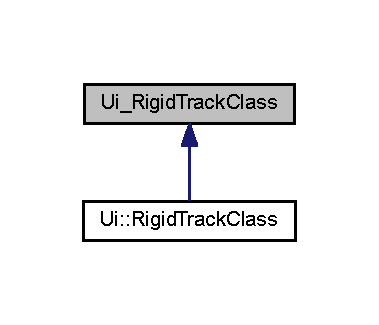
\includegraphics[width=182pt]{class_ui___rigid_track_class__inherit__graph}
\end{center}
\end{figure}
\subsection*{Public Member Functions}
\begin{DoxyCompactItemize}
\item 
void \hyperlink{class_ui___rigid_track_class_a7f78fefc15716049b873bef4d3450e38}{setup\+Ui} (Q\+Main\+Window $\ast$Rigid\+Track\+Class)
\item 
void \hyperlink{class_ui___rigid_track_class_a7c96951c4e173848e7695d6bd7883af6}{retranslate\+Ui} (Q\+Main\+Window $\ast$Rigid\+Track\+Class)
\begin{DoxyCompactList}\small\item\em /$<$ setup\+Ui \end{DoxyCompactList}\end{DoxyCompactItemize}
\subsection*{Public Attributes}
\begin{DoxyCompactItemize}
\item 
Q\+Action $\ast$ \hyperlink{class_ui___rigid_track_class_aeb9fefc5e71112c520ae22f6e818d01f}{action\+Show\+\_\+\+Help}
\item 
Q\+Action $\ast$ \hyperlink{class_ui___rigid_track_class_a3fb674ec6f96c57d3eef03900b7162ba}{action\+Open\+\_\+\+Log\+\_\+\+Folder}
\item 
Q\+Action $\ast$ \hyperlink{class_ui___rigid_track_class_adbf50ad17608dbfe8a688dc8f18d1ec3}{action\+Open\+\_\+\+Installation\+\_\+\+Folder}
\item 
Q\+Widget $\ast$ \hyperlink{class_ui___rigid_track_class_ad0855ddf1efd8f0c8821dd2142f6221d}{central\+Widget}
\item 
Q\+Push\+Button $\ast$ \hyperlink{class_ui___rigid_track_class_a72fc55bdb6021b52b9ec0e97e112d57d}{btn\+Start\+Camera}
\item 
Q\+Label $\ast$ \hyperlink{class_ui___rigid_track_class_abeac37c5be33dbe8f2805a9e688b8329}{lb\+Status}
\item 
Q\+Push\+Button $\ast$ \hyperlink{class_ui___rigid_track_class_acc37707b26574be199e2f33d2f2c31fe}{btn\+Zero}
\item 
Q\+Push\+Button $\ast$ \hyperlink{class_ui___rigid_track_class_aac22c36a194fd08f919a8e00a78cb1b0}{btn\+Calibrate}
\item 
Q\+Push\+Button $\ast$ \hyperlink{class_ui___rigid_track_class_aafe138bcd4b21e4608ab39f76ca6e042}{btn\+Load\+Calib}
\item 
Q\+List\+Widget $\ast$ \hyperlink{class_ui___rigid_track_class_a8573490fa3f39f7c45af77f33c9b9297}{list\+Log}
\item 
Q\+Double\+Spin\+Box $\ast$ \hyperlink{class_ui___rigid_track_class_a7a9db994f872078ce46a81b435f70cf9}{sb\+Heading\+Offset}
\item 
Q\+Label $\ast$ \hyperlink{class_ui___rigid_track_class_a2de57788f55b334c451dc9d0449b104c}{label}
\item 
Q\+Line\+Edit $\ast$ \hyperlink{class_ui___rigid_track_class_a8372ffd3f54aa2672228e28e48fe18f3}{le\+I\+P\+Object}
\item 
Q\+Label $\ast$ \hyperlink{class_ui___rigid_track_class_adad99dbe226b6a900918729abb37a6b8}{label\+\_\+2}
\item 
Q\+Group\+Box $\ast$ \hyperlink{class_ui___rigid_track_class_a895128ce9cc7dda6c57b654512e12e7d}{group\+Box}
\item 
Q\+Radio\+Button $\ast$ \hyperlink{class_ui___rigid_track_class_a7ee2c6448b82ecb455b4f6122ea8dbeb}{rb\+Iterative}
\item 
Q\+Radio\+Button $\ast$ \hyperlink{class_ui___rigid_track_class_a3f20a41a0b0d35ff5a077530743c82c9}{rb\+P3P}
\item 
Q\+Radio\+Button $\ast$ \hyperlink{class_ui___rigid_track_class_a1c45060b8c85c0e4cfe4a7c1e40f203a}{rb\+E\+PnP}
\item 
Q\+Group\+Box $\ast$ \hyperlink{class_ui___rigid_track_class_a85d7c172656cb175131c5da83caf6a48}{group\+Box\+\_\+2}
\item 
Q\+Check\+Box $\ast$ \hyperlink{class_ui___rigid_track_class_a44e812df547a219bdf2b43383a4e849b}{cb\+Safety}
\item 
Q\+Double\+Spin\+Box $\ast$ \hyperlink{class_ui___rigid_track_class_a20f78b58534d29da3d836c2af79a6232}{dsb\+Dimension}
\item 
Q\+Spin\+Box $\ast$ \hyperlink{class_ui___rigid_track_class_ac232f3d19d53b00aa61431725cbf71c4}{sb\+Angle}
\item 
Q\+Label $\ast$ \hyperlink{class_ui___rigid_track_class_a0996dad75e113e08fcaee07e55ceaca6}{lb\+Safety\+Area}
\item 
Q\+Label $\ast$ \hyperlink{class_ui___rigid_track_class_ace9b8966d2c9a38ef4bd4ba17db70c5a}{lb\+Safety\+Area\+\_\+2}
\item 
Q\+Line\+Edit $\ast$ \hyperlink{class_ui___rigid_track_class_af722611603b357175b3ce505bdf468b1}{le\+I\+P\+Safety}
\item 
Q\+Label $\ast$ \hyperlink{class_ui___rigid_track_class_a40dc760bee515c66ebe81f67b2d7f5f9}{label\+\_\+3}
\item 
Q\+Push\+Button $\ast$ \hyperlink{class_ui___rigid_track_class_a76c00d83ae38b7eaa03ef28c280631fa}{pb\+Load\+Marker}
\item 
Q\+Group\+Box $\ast$ \hyperlink{class_ui___rigid_track_class_a822d802011c4868603863fa70f5589ae}{group\+Box\+\_\+3}
\item 
Q\+Check\+Box $\ast$ \hyperlink{class_ui___rigid_track_class_a1e5273e53cb1276c8c056f1da4e72910}{cb\+Safety2}
\item 
Q\+Line\+Edit $\ast$ \hyperlink{class_ui___rigid_track_class_a70522f29594cbdc654ffed858b3e1fc5}{le\+I\+P\+Safety2}
\item 
Q\+Check\+Box $\ast$ \hyperlink{class_ui___rigid_track_class_a370014fb6d177a07220b69155b4c101b}{cb\+Invert}
\item 
Q\+Progress\+Bar $\ast$ \hyperlink{class_ui___rigid_track_class_a4f53c207d82dc9555709f1ace400d89b}{progress\+Bar}
\item 
Q\+Push\+Button $\ast$ \hyperlink{class_ui___rigid_track_class_a7497d27bfd5a03243079fdb055291264}{btn\+Calibrate\+Ground}
\item 
Q\+Menu\+Bar $\ast$ \hyperlink{class_ui___rigid_track_class_ae5991e1872fe74ac542cf0fdca8d4d0e}{menu\+Bar}
\item 
Q\+Menu $\ast$ \hyperlink{class_ui___rigid_track_class_a2df43c6bb7db7e366a64bc8dbbbab7cc}{menu\+Help}
\item 
Q\+Menu $\ast$ \hyperlink{class_ui___rigid_track_class_a1df91ff9df043558cf6d3c1dd6557250}{menu\+Open\+\_\+\+Logs}
\item 
Q\+Tool\+Bar $\ast$ \hyperlink{class_ui___rigid_track_class_abb7105788d67491618ebd4229964f992}{main\+Tool\+Bar}
\item 
Q\+Status\+Bar $\ast$ \hyperlink{class_ui___rigid_track_class_ac1ced4ae725bc0095307704d5d4fc4f2}{status\+Bar}
\end{DoxyCompactItemize}


\subsection{Member Function Documentation}
\mbox{\Hypertarget{class_ui___rigid_track_class_a7c96951c4e173848e7695d6bd7883af6}\label{class_ui___rigid_track_class_a7c96951c4e173848e7695d6bd7883af6}} 
\index{Ui\+\_\+\+Rigid\+Track\+Class@{Ui\+\_\+\+Rigid\+Track\+Class}!retranslate\+Ui@{retranslate\+Ui}}
\index{retranslate\+Ui@{retranslate\+Ui}!Ui\+\_\+\+Rigid\+Track\+Class@{Ui\+\_\+\+Rigid\+Track\+Class}}
\subsubsection{\texorpdfstring{retranslate\+Ui()}{retranslateUi()}}
{\footnotesize\ttfamily void Ui\+\_\+\+Rigid\+Track\+Class\+::retranslate\+Ui (\begin{DoxyParamCaption}\item[{Q\+Main\+Window $\ast$}]{Rigid\+Track\+Class }\end{DoxyParamCaption})\hspace{0.3cm}{\ttfamily [inline]}}



/$<$ setup\+Ui 

/$<$ Q\+T\+\_\+\+N\+O\+\_\+\+T\+O\+O\+L\+T\+IP

/$<$ Q\+T\+\_\+\+N\+O\+\_\+\+T\+O\+O\+L\+T\+IP

/$<$ Q\+T\+\_\+\+N\+O\+\_\+\+T\+O\+O\+L\+T\+IP

/$<$ Q\+T\+\_\+\+N\+O\+\_\+\+T\+O\+O\+L\+T\+IP

/$<$ Q\+T\+\_\+\+N\+O\+\_\+\+T\+O\+O\+L\+T\+IP

/$<$ Q\+T\+\_\+\+N\+O\+\_\+\+T\+O\+O\+L\+T\+IP Here is the caller graph for this function\+:\nopagebreak
\begin{figure}[H]
\begin{center}
\leavevmode
\includegraphics[width=350pt]{class_ui___rigid_track_class_a7c96951c4e173848e7695d6bd7883af6_icgraph}
\end{center}
\end{figure}
\mbox{\Hypertarget{class_ui___rigid_track_class_a7f78fefc15716049b873bef4d3450e38}\label{class_ui___rigid_track_class_a7f78fefc15716049b873bef4d3450e38}} 
\index{Ui\+\_\+\+Rigid\+Track\+Class@{Ui\+\_\+\+Rigid\+Track\+Class}!setup\+Ui@{setup\+Ui}}
\index{setup\+Ui@{setup\+Ui}!Ui\+\_\+\+Rigid\+Track\+Class@{Ui\+\_\+\+Rigid\+Track\+Class}}
\subsubsection{\texorpdfstring{setup\+Ui()}{setupUi()}}
{\footnotesize\ttfamily void Ui\+\_\+\+Rigid\+Track\+Class\+::setup\+Ui (\begin{DoxyParamCaption}\item[{Q\+Main\+Window $\ast$}]{Rigid\+Track\+Class }\end{DoxyParamCaption})\hspace{0.3cm}{\ttfamily [inline]}}

Here is the call graph for this function\+:\nopagebreak
\begin{figure}[H]
\begin{center}
\leavevmode
\includegraphics[width=318pt]{class_ui___rigid_track_class_a7f78fefc15716049b873bef4d3450e38_cgraph}
\end{center}
\end{figure}
Here is the caller graph for this function\+:\nopagebreak
\begin{figure}[H]
\begin{center}
\leavevmode
\includegraphics[width=331pt]{class_ui___rigid_track_class_a7f78fefc15716049b873bef4d3450e38_icgraph}
\end{center}
\end{figure}


\subsection{Member Data Documentation}
\mbox{\Hypertarget{class_ui___rigid_track_class_adbf50ad17608dbfe8a688dc8f18d1ec3}\label{class_ui___rigid_track_class_adbf50ad17608dbfe8a688dc8f18d1ec3}} 
\index{Ui\+\_\+\+Rigid\+Track\+Class@{Ui\+\_\+\+Rigid\+Track\+Class}!action\+Open\+\_\+\+Installation\+\_\+\+Folder@{action\+Open\+\_\+\+Installation\+\_\+\+Folder}}
\index{action\+Open\+\_\+\+Installation\+\_\+\+Folder@{action\+Open\+\_\+\+Installation\+\_\+\+Folder}!Ui\+\_\+\+Rigid\+Track\+Class@{Ui\+\_\+\+Rigid\+Track\+Class}}
\subsubsection{\texorpdfstring{action\+Open\+\_\+\+Installation\+\_\+\+Folder}{actionOpen\_Installation\_Folder}}
{\footnotesize\ttfamily Q\+Action$\ast$ Ui\+\_\+\+Rigid\+Track\+Class\+::action\+Open\+\_\+\+Installation\+\_\+\+Folder}

\mbox{\Hypertarget{class_ui___rigid_track_class_a3fb674ec6f96c57d3eef03900b7162ba}\label{class_ui___rigid_track_class_a3fb674ec6f96c57d3eef03900b7162ba}} 
\index{Ui\+\_\+\+Rigid\+Track\+Class@{Ui\+\_\+\+Rigid\+Track\+Class}!action\+Open\+\_\+\+Log\+\_\+\+Folder@{action\+Open\+\_\+\+Log\+\_\+\+Folder}}
\index{action\+Open\+\_\+\+Log\+\_\+\+Folder@{action\+Open\+\_\+\+Log\+\_\+\+Folder}!Ui\+\_\+\+Rigid\+Track\+Class@{Ui\+\_\+\+Rigid\+Track\+Class}}
\subsubsection{\texorpdfstring{action\+Open\+\_\+\+Log\+\_\+\+Folder}{actionOpen\_Log\_Folder}}
{\footnotesize\ttfamily Q\+Action$\ast$ Ui\+\_\+\+Rigid\+Track\+Class\+::action\+Open\+\_\+\+Log\+\_\+\+Folder}

\mbox{\Hypertarget{class_ui___rigid_track_class_aeb9fefc5e71112c520ae22f6e818d01f}\label{class_ui___rigid_track_class_aeb9fefc5e71112c520ae22f6e818d01f}} 
\index{Ui\+\_\+\+Rigid\+Track\+Class@{Ui\+\_\+\+Rigid\+Track\+Class}!action\+Show\+\_\+\+Help@{action\+Show\+\_\+\+Help}}
\index{action\+Show\+\_\+\+Help@{action\+Show\+\_\+\+Help}!Ui\+\_\+\+Rigid\+Track\+Class@{Ui\+\_\+\+Rigid\+Track\+Class}}
\subsubsection{\texorpdfstring{action\+Show\+\_\+\+Help}{actionShow\_Help}}
{\footnotesize\ttfamily Q\+Action$\ast$ Ui\+\_\+\+Rigid\+Track\+Class\+::action\+Show\+\_\+\+Help}

\mbox{\Hypertarget{class_ui___rigid_track_class_aac22c36a194fd08f919a8e00a78cb1b0}\label{class_ui___rigid_track_class_aac22c36a194fd08f919a8e00a78cb1b0}} 
\index{Ui\+\_\+\+Rigid\+Track\+Class@{Ui\+\_\+\+Rigid\+Track\+Class}!btn\+Calibrate@{btn\+Calibrate}}
\index{btn\+Calibrate@{btn\+Calibrate}!Ui\+\_\+\+Rigid\+Track\+Class@{Ui\+\_\+\+Rigid\+Track\+Class}}
\subsubsection{\texorpdfstring{btn\+Calibrate}{btnCalibrate}}
{\footnotesize\ttfamily Q\+Push\+Button$\ast$ Ui\+\_\+\+Rigid\+Track\+Class\+::btn\+Calibrate}

\mbox{\Hypertarget{class_ui___rigid_track_class_a7497d27bfd5a03243079fdb055291264}\label{class_ui___rigid_track_class_a7497d27bfd5a03243079fdb055291264}} 
\index{Ui\+\_\+\+Rigid\+Track\+Class@{Ui\+\_\+\+Rigid\+Track\+Class}!btn\+Calibrate\+Ground@{btn\+Calibrate\+Ground}}
\index{btn\+Calibrate\+Ground@{btn\+Calibrate\+Ground}!Ui\+\_\+\+Rigid\+Track\+Class@{Ui\+\_\+\+Rigid\+Track\+Class}}
\subsubsection{\texorpdfstring{btn\+Calibrate\+Ground}{btnCalibrateGround}}
{\footnotesize\ttfamily Q\+Push\+Button$\ast$ Ui\+\_\+\+Rigid\+Track\+Class\+::btn\+Calibrate\+Ground}

\mbox{\Hypertarget{class_ui___rigid_track_class_aafe138bcd4b21e4608ab39f76ca6e042}\label{class_ui___rigid_track_class_aafe138bcd4b21e4608ab39f76ca6e042}} 
\index{Ui\+\_\+\+Rigid\+Track\+Class@{Ui\+\_\+\+Rigid\+Track\+Class}!btn\+Load\+Calib@{btn\+Load\+Calib}}
\index{btn\+Load\+Calib@{btn\+Load\+Calib}!Ui\+\_\+\+Rigid\+Track\+Class@{Ui\+\_\+\+Rigid\+Track\+Class}}
\subsubsection{\texorpdfstring{btn\+Load\+Calib}{btnLoadCalib}}
{\footnotesize\ttfamily Q\+Push\+Button$\ast$ Ui\+\_\+\+Rigid\+Track\+Class\+::btn\+Load\+Calib}

\mbox{\Hypertarget{class_ui___rigid_track_class_a72fc55bdb6021b52b9ec0e97e112d57d}\label{class_ui___rigid_track_class_a72fc55bdb6021b52b9ec0e97e112d57d}} 
\index{Ui\+\_\+\+Rigid\+Track\+Class@{Ui\+\_\+\+Rigid\+Track\+Class}!btn\+Start\+Camera@{btn\+Start\+Camera}}
\index{btn\+Start\+Camera@{btn\+Start\+Camera}!Ui\+\_\+\+Rigid\+Track\+Class@{Ui\+\_\+\+Rigid\+Track\+Class}}
\subsubsection{\texorpdfstring{btn\+Start\+Camera}{btnStartCamera}}
{\footnotesize\ttfamily Q\+Push\+Button$\ast$ Ui\+\_\+\+Rigid\+Track\+Class\+::btn\+Start\+Camera}

\mbox{\Hypertarget{class_ui___rigid_track_class_acc37707b26574be199e2f33d2f2c31fe}\label{class_ui___rigid_track_class_acc37707b26574be199e2f33d2f2c31fe}} 
\index{Ui\+\_\+\+Rigid\+Track\+Class@{Ui\+\_\+\+Rigid\+Track\+Class}!btn\+Zero@{btn\+Zero}}
\index{btn\+Zero@{btn\+Zero}!Ui\+\_\+\+Rigid\+Track\+Class@{Ui\+\_\+\+Rigid\+Track\+Class}}
\subsubsection{\texorpdfstring{btn\+Zero}{btnZero}}
{\footnotesize\ttfamily Q\+Push\+Button$\ast$ Ui\+\_\+\+Rigid\+Track\+Class\+::btn\+Zero}

\mbox{\Hypertarget{class_ui___rigid_track_class_a370014fb6d177a07220b69155b4c101b}\label{class_ui___rigid_track_class_a370014fb6d177a07220b69155b4c101b}} 
\index{Ui\+\_\+\+Rigid\+Track\+Class@{Ui\+\_\+\+Rigid\+Track\+Class}!cb\+Invert@{cb\+Invert}}
\index{cb\+Invert@{cb\+Invert}!Ui\+\_\+\+Rigid\+Track\+Class@{Ui\+\_\+\+Rigid\+Track\+Class}}
\subsubsection{\texorpdfstring{cb\+Invert}{cbInvert}}
{\footnotesize\ttfamily Q\+Check\+Box$\ast$ Ui\+\_\+\+Rigid\+Track\+Class\+::cb\+Invert}

\mbox{\Hypertarget{class_ui___rigid_track_class_a44e812df547a219bdf2b43383a4e849b}\label{class_ui___rigid_track_class_a44e812df547a219bdf2b43383a4e849b}} 
\index{Ui\+\_\+\+Rigid\+Track\+Class@{Ui\+\_\+\+Rigid\+Track\+Class}!cb\+Safety@{cb\+Safety}}
\index{cb\+Safety@{cb\+Safety}!Ui\+\_\+\+Rigid\+Track\+Class@{Ui\+\_\+\+Rigid\+Track\+Class}}
\subsubsection{\texorpdfstring{cb\+Safety}{cbSafety}}
{\footnotesize\ttfamily Q\+Check\+Box$\ast$ Ui\+\_\+\+Rigid\+Track\+Class\+::cb\+Safety}

\mbox{\Hypertarget{class_ui___rigid_track_class_a1e5273e53cb1276c8c056f1da4e72910}\label{class_ui___rigid_track_class_a1e5273e53cb1276c8c056f1da4e72910}} 
\index{Ui\+\_\+\+Rigid\+Track\+Class@{Ui\+\_\+\+Rigid\+Track\+Class}!cb\+Safety2@{cb\+Safety2}}
\index{cb\+Safety2@{cb\+Safety2}!Ui\+\_\+\+Rigid\+Track\+Class@{Ui\+\_\+\+Rigid\+Track\+Class}}
\subsubsection{\texorpdfstring{cb\+Safety2}{cbSafety2}}
{\footnotesize\ttfamily Q\+Check\+Box$\ast$ Ui\+\_\+\+Rigid\+Track\+Class\+::cb\+Safety2}

\mbox{\Hypertarget{class_ui___rigid_track_class_ad0855ddf1efd8f0c8821dd2142f6221d}\label{class_ui___rigid_track_class_ad0855ddf1efd8f0c8821dd2142f6221d}} 
\index{Ui\+\_\+\+Rigid\+Track\+Class@{Ui\+\_\+\+Rigid\+Track\+Class}!central\+Widget@{central\+Widget}}
\index{central\+Widget@{central\+Widget}!Ui\+\_\+\+Rigid\+Track\+Class@{Ui\+\_\+\+Rigid\+Track\+Class}}
\subsubsection{\texorpdfstring{central\+Widget}{centralWidget}}
{\footnotesize\ttfamily Q\+Widget$\ast$ Ui\+\_\+\+Rigid\+Track\+Class\+::central\+Widget}

\mbox{\Hypertarget{class_ui___rigid_track_class_a20f78b58534d29da3d836c2af79a6232}\label{class_ui___rigid_track_class_a20f78b58534d29da3d836c2af79a6232}} 
\index{Ui\+\_\+\+Rigid\+Track\+Class@{Ui\+\_\+\+Rigid\+Track\+Class}!dsb\+Dimension@{dsb\+Dimension}}
\index{dsb\+Dimension@{dsb\+Dimension}!Ui\+\_\+\+Rigid\+Track\+Class@{Ui\+\_\+\+Rigid\+Track\+Class}}
\subsubsection{\texorpdfstring{dsb\+Dimension}{dsbDimension}}
{\footnotesize\ttfamily Q\+Double\+Spin\+Box$\ast$ Ui\+\_\+\+Rigid\+Track\+Class\+::dsb\+Dimension}

\mbox{\Hypertarget{class_ui___rigid_track_class_a895128ce9cc7dda6c57b654512e12e7d}\label{class_ui___rigid_track_class_a895128ce9cc7dda6c57b654512e12e7d}} 
\index{Ui\+\_\+\+Rigid\+Track\+Class@{Ui\+\_\+\+Rigid\+Track\+Class}!group\+Box@{group\+Box}}
\index{group\+Box@{group\+Box}!Ui\+\_\+\+Rigid\+Track\+Class@{Ui\+\_\+\+Rigid\+Track\+Class}}
\subsubsection{\texorpdfstring{group\+Box}{groupBox}}
{\footnotesize\ttfamily Q\+Group\+Box$\ast$ Ui\+\_\+\+Rigid\+Track\+Class\+::group\+Box}

\mbox{\Hypertarget{class_ui___rigid_track_class_a85d7c172656cb175131c5da83caf6a48}\label{class_ui___rigid_track_class_a85d7c172656cb175131c5da83caf6a48}} 
\index{Ui\+\_\+\+Rigid\+Track\+Class@{Ui\+\_\+\+Rigid\+Track\+Class}!group\+Box\+\_\+2@{group\+Box\+\_\+2}}
\index{group\+Box\+\_\+2@{group\+Box\+\_\+2}!Ui\+\_\+\+Rigid\+Track\+Class@{Ui\+\_\+\+Rigid\+Track\+Class}}
\subsubsection{\texorpdfstring{group\+Box\+\_\+2}{groupBox\_2}}
{\footnotesize\ttfamily Q\+Group\+Box$\ast$ Ui\+\_\+\+Rigid\+Track\+Class\+::group\+Box\+\_\+2}

\mbox{\Hypertarget{class_ui___rigid_track_class_a822d802011c4868603863fa70f5589ae}\label{class_ui___rigid_track_class_a822d802011c4868603863fa70f5589ae}} 
\index{Ui\+\_\+\+Rigid\+Track\+Class@{Ui\+\_\+\+Rigid\+Track\+Class}!group\+Box\+\_\+3@{group\+Box\+\_\+3}}
\index{group\+Box\+\_\+3@{group\+Box\+\_\+3}!Ui\+\_\+\+Rigid\+Track\+Class@{Ui\+\_\+\+Rigid\+Track\+Class}}
\subsubsection{\texorpdfstring{group\+Box\+\_\+3}{groupBox\_3}}
{\footnotesize\ttfamily Q\+Group\+Box$\ast$ Ui\+\_\+\+Rigid\+Track\+Class\+::group\+Box\+\_\+3}

\mbox{\Hypertarget{class_ui___rigid_track_class_a2de57788f55b334c451dc9d0449b104c}\label{class_ui___rigid_track_class_a2de57788f55b334c451dc9d0449b104c}} 
\index{Ui\+\_\+\+Rigid\+Track\+Class@{Ui\+\_\+\+Rigid\+Track\+Class}!label@{label}}
\index{label@{label}!Ui\+\_\+\+Rigid\+Track\+Class@{Ui\+\_\+\+Rigid\+Track\+Class}}
\subsubsection{\texorpdfstring{label}{label}}
{\footnotesize\ttfamily Q\+Label$\ast$ Ui\+\_\+\+Rigid\+Track\+Class\+::label}

\mbox{\Hypertarget{class_ui___rigid_track_class_adad99dbe226b6a900918729abb37a6b8}\label{class_ui___rigid_track_class_adad99dbe226b6a900918729abb37a6b8}} 
\index{Ui\+\_\+\+Rigid\+Track\+Class@{Ui\+\_\+\+Rigid\+Track\+Class}!label\+\_\+2@{label\+\_\+2}}
\index{label\+\_\+2@{label\+\_\+2}!Ui\+\_\+\+Rigid\+Track\+Class@{Ui\+\_\+\+Rigid\+Track\+Class}}
\subsubsection{\texorpdfstring{label\+\_\+2}{label\_2}}
{\footnotesize\ttfamily Q\+Label$\ast$ Ui\+\_\+\+Rigid\+Track\+Class\+::label\+\_\+2}

\mbox{\Hypertarget{class_ui___rigid_track_class_a40dc760bee515c66ebe81f67b2d7f5f9}\label{class_ui___rigid_track_class_a40dc760bee515c66ebe81f67b2d7f5f9}} 
\index{Ui\+\_\+\+Rigid\+Track\+Class@{Ui\+\_\+\+Rigid\+Track\+Class}!label\+\_\+3@{label\+\_\+3}}
\index{label\+\_\+3@{label\+\_\+3}!Ui\+\_\+\+Rigid\+Track\+Class@{Ui\+\_\+\+Rigid\+Track\+Class}}
\subsubsection{\texorpdfstring{label\+\_\+3}{label\_3}}
{\footnotesize\ttfamily Q\+Label$\ast$ Ui\+\_\+\+Rigid\+Track\+Class\+::label\+\_\+3}

\mbox{\Hypertarget{class_ui___rigid_track_class_a0996dad75e113e08fcaee07e55ceaca6}\label{class_ui___rigid_track_class_a0996dad75e113e08fcaee07e55ceaca6}} 
\index{Ui\+\_\+\+Rigid\+Track\+Class@{Ui\+\_\+\+Rigid\+Track\+Class}!lb\+Safety\+Area@{lb\+Safety\+Area}}
\index{lb\+Safety\+Area@{lb\+Safety\+Area}!Ui\+\_\+\+Rigid\+Track\+Class@{Ui\+\_\+\+Rigid\+Track\+Class}}
\subsubsection{\texorpdfstring{lb\+Safety\+Area}{lbSafetyArea}}
{\footnotesize\ttfamily Q\+Label$\ast$ Ui\+\_\+\+Rigid\+Track\+Class\+::lb\+Safety\+Area}

\mbox{\Hypertarget{class_ui___rigid_track_class_ace9b8966d2c9a38ef4bd4ba17db70c5a}\label{class_ui___rigid_track_class_ace9b8966d2c9a38ef4bd4ba17db70c5a}} 
\index{Ui\+\_\+\+Rigid\+Track\+Class@{Ui\+\_\+\+Rigid\+Track\+Class}!lb\+Safety\+Area\+\_\+2@{lb\+Safety\+Area\+\_\+2}}
\index{lb\+Safety\+Area\+\_\+2@{lb\+Safety\+Area\+\_\+2}!Ui\+\_\+\+Rigid\+Track\+Class@{Ui\+\_\+\+Rigid\+Track\+Class}}
\subsubsection{\texorpdfstring{lb\+Safety\+Area\+\_\+2}{lbSafetyArea\_2}}
{\footnotesize\ttfamily Q\+Label$\ast$ Ui\+\_\+\+Rigid\+Track\+Class\+::lb\+Safety\+Area\+\_\+2}

\mbox{\Hypertarget{class_ui___rigid_track_class_abeac37c5be33dbe8f2805a9e688b8329}\label{class_ui___rigid_track_class_abeac37c5be33dbe8f2805a9e688b8329}} 
\index{Ui\+\_\+\+Rigid\+Track\+Class@{Ui\+\_\+\+Rigid\+Track\+Class}!lb\+Status@{lb\+Status}}
\index{lb\+Status@{lb\+Status}!Ui\+\_\+\+Rigid\+Track\+Class@{Ui\+\_\+\+Rigid\+Track\+Class}}
\subsubsection{\texorpdfstring{lb\+Status}{lbStatus}}
{\footnotesize\ttfamily Q\+Label$\ast$ Ui\+\_\+\+Rigid\+Track\+Class\+::lb\+Status}

\mbox{\Hypertarget{class_ui___rigid_track_class_a8372ffd3f54aa2672228e28e48fe18f3}\label{class_ui___rigid_track_class_a8372ffd3f54aa2672228e28e48fe18f3}} 
\index{Ui\+\_\+\+Rigid\+Track\+Class@{Ui\+\_\+\+Rigid\+Track\+Class}!le\+I\+P\+Object@{le\+I\+P\+Object}}
\index{le\+I\+P\+Object@{le\+I\+P\+Object}!Ui\+\_\+\+Rigid\+Track\+Class@{Ui\+\_\+\+Rigid\+Track\+Class}}
\subsubsection{\texorpdfstring{le\+I\+P\+Object}{leIPObject}}
{\footnotesize\ttfamily Q\+Line\+Edit$\ast$ Ui\+\_\+\+Rigid\+Track\+Class\+::le\+I\+P\+Object}

\mbox{\Hypertarget{class_ui___rigid_track_class_af722611603b357175b3ce505bdf468b1}\label{class_ui___rigid_track_class_af722611603b357175b3ce505bdf468b1}} 
\index{Ui\+\_\+\+Rigid\+Track\+Class@{Ui\+\_\+\+Rigid\+Track\+Class}!le\+I\+P\+Safety@{le\+I\+P\+Safety}}
\index{le\+I\+P\+Safety@{le\+I\+P\+Safety}!Ui\+\_\+\+Rigid\+Track\+Class@{Ui\+\_\+\+Rigid\+Track\+Class}}
\subsubsection{\texorpdfstring{le\+I\+P\+Safety}{leIPSafety}}
{\footnotesize\ttfamily Q\+Line\+Edit$\ast$ Ui\+\_\+\+Rigid\+Track\+Class\+::le\+I\+P\+Safety}

\mbox{\Hypertarget{class_ui___rigid_track_class_a70522f29594cbdc654ffed858b3e1fc5}\label{class_ui___rigid_track_class_a70522f29594cbdc654ffed858b3e1fc5}} 
\index{Ui\+\_\+\+Rigid\+Track\+Class@{Ui\+\_\+\+Rigid\+Track\+Class}!le\+I\+P\+Safety2@{le\+I\+P\+Safety2}}
\index{le\+I\+P\+Safety2@{le\+I\+P\+Safety2}!Ui\+\_\+\+Rigid\+Track\+Class@{Ui\+\_\+\+Rigid\+Track\+Class}}
\subsubsection{\texorpdfstring{le\+I\+P\+Safety2}{leIPSafety2}}
{\footnotesize\ttfamily Q\+Line\+Edit$\ast$ Ui\+\_\+\+Rigid\+Track\+Class\+::le\+I\+P\+Safety2}

\mbox{\Hypertarget{class_ui___rigid_track_class_a8573490fa3f39f7c45af77f33c9b9297}\label{class_ui___rigid_track_class_a8573490fa3f39f7c45af77f33c9b9297}} 
\index{Ui\+\_\+\+Rigid\+Track\+Class@{Ui\+\_\+\+Rigid\+Track\+Class}!list\+Log@{list\+Log}}
\index{list\+Log@{list\+Log}!Ui\+\_\+\+Rigid\+Track\+Class@{Ui\+\_\+\+Rigid\+Track\+Class}}
\subsubsection{\texorpdfstring{list\+Log}{listLog}}
{\footnotesize\ttfamily Q\+List\+Widget$\ast$ Ui\+\_\+\+Rigid\+Track\+Class\+::list\+Log}

\mbox{\Hypertarget{class_ui___rigid_track_class_abb7105788d67491618ebd4229964f992}\label{class_ui___rigid_track_class_abb7105788d67491618ebd4229964f992}} 
\index{Ui\+\_\+\+Rigid\+Track\+Class@{Ui\+\_\+\+Rigid\+Track\+Class}!main\+Tool\+Bar@{main\+Tool\+Bar}}
\index{main\+Tool\+Bar@{main\+Tool\+Bar}!Ui\+\_\+\+Rigid\+Track\+Class@{Ui\+\_\+\+Rigid\+Track\+Class}}
\subsubsection{\texorpdfstring{main\+Tool\+Bar}{mainToolBar}}
{\footnotesize\ttfamily Q\+Tool\+Bar$\ast$ Ui\+\_\+\+Rigid\+Track\+Class\+::main\+Tool\+Bar}

\mbox{\Hypertarget{class_ui___rigid_track_class_ae5991e1872fe74ac542cf0fdca8d4d0e}\label{class_ui___rigid_track_class_ae5991e1872fe74ac542cf0fdca8d4d0e}} 
\index{Ui\+\_\+\+Rigid\+Track\+Class@{Ui\+\_\+\+Rigid\+Track\+Class}!menu\+Bar@{menu\+Bar}}
\index{menu\+Bar@{menu\+Bar}!Ui\+\_\+\+Rigid\+Track\+Class@{Ui\+\_\+\+Rigid\+Track\+Class}}
\subsubsection{\texorpdfstring{menu\+Bar}{menuBar}}
{\footnotesize\ttfamily Q\+Menu\+Bar$\ast$ Ui\+\_\+\+Rigid\+Track\+Class\+::menu\+Bar}

\mbox{\Hypertarget{class_ui___rigid_track_class_a2df43c6bb7db7e366a64bc8dbbbab7cc}\label{class_ui___rigid_track_class_a2df43c6bb7db7e366a64bc8dbbbab7cc}} 
\index{Ui\+\_\+\+Rigid\+Track\+Class@{Ui\+\_\+\+Rigid\+Track\+Class}!menu\+Help@{menu\+Help}}
\index{menu\+Help@{menu\+Help}!Ui\+\_\+\+Rigid\+Track\+Class@{Ui\+\_\+\+Rigid\+Track\+Class}}
\subsubsection{\texorpdfstring{menu\+Help}{menuHelp}}
{\footnotesize\ttfamily Q\+Menu$\ast$ Ui\+\_\+\+Rigid\+Track\+Class\+::menu\+Help}

\mbox{\Hypertarget{class_ui___rigid_track_class_a1df91ff9df043558cf6d3c1dd6557250}\label{class_ui___rigid_track_class_a1df91ff9df043558cf6d3c1dd6557250}} 
\index{Ui\+\_\+\+Rigid\+Track\+Class@{Ui\+\_\+\+Rigid\+Track\+Class}!menu\+Open\+\_\+\+Logs@{menu\+Open\+\_\+\+Logs}}
\index{menu\+Open\+\_\+\+Logs@{menu\+Open\+\_\+\+Logs}!Ui\+\_\+\+Rigid\+Track\+Class@{Ui\+\_\+\+Rigid\+Track\+Class}}
\subsubsection{\texorpdfstring{menu\+Open\+\_\+\+Logs}{menuOpen\_Logs}}
{\footnotesize\ttfamily Q\+Menu$\ast$ Ui\+\_\+\+Rigid\+Track\+Class\+::menu\+Open\+\_\+\+Logs}

\mbox{\Hypertarget{class_ui___rigid_track_class_a76c00d83ae38b7eaa03ef28c280631fa}\label{class_ui___rigid_track_class_a76c00d83ae38b7eaa03ef28c280631fa}} 
\index{Ui\+\_\+\+Rigid\+Track\+Class@{Ui\+\_\+\+Rigid\+Track\+Class}!pb\+Load\+Marker@{pb\+Load\+Marker}}
\index{pb\+Load\+Marker@{pb\+Load\+Marker}!Ui\+\_\+\+Rigid\+Track\+Class@{Ui\+\_\+\+Rigid\+Track\+Class}}
\subsubsection{\texorpdfstring{pb\+Load\+Marker}{pbLoadMarker}}
{\footnotesize\ttfamily Q\+Push\+Button$\ast$ Ui\+\_\+\+Rigid\+Track\+Class\+::pb\+Load\+Marker}

\mbox{\Hypertarget{class_ui___rigid_track_class_a4f53c207d82dc9555709f1ace400d89b}\label{class_ui___rigid_track_class_a4f53c207d82dc9555709f1ace400d89b}} 
\index{Ui\+\_\+\+Rigid\+Track\+Class@{Ui\+\_\+\+Rigid\+Track\+Class}!progress\+Bar@{progress\+Bar}}
\index{progress\+Bar@{progress\+Bar}!Ui\+\_\+\+Rigid\+Track\+Class@{Ui\+\_\+\+Rigid\+Track\+Class}}
\subsubsection{\texorpdfstring{progress\+Bar}{progressBar}}
{\footnotesize\ttfamily Q\+Progress\+Bar$\ast$ Ui\+\_\+\+Rigid\+Track\+Class\+::progress\+Bar}

\mbox{\Hypertarget{class_ui___rigid_track_class_a1c45060b8c85c0e4cfe4a7c1e40f203a}\label{class_ui___rigid_track_class_a1c45060b8c85c0e4cfe4a7c1e40f203a}} 
\index{Ui\+\_\+\+Rigid\+Track\+Class@{Ui\+\_\+\+Rigid\+Track\+Class}!rb\+E\+PnP@{rb\+E\+PnP}}
\index{rb\+E\+PnP@{rb\+E\+PnP}!Ui\+\_\+\+Rigid\+Track\+Class@{Ui\+\_\+\+Rigid\+Track\+Class}}
\subsubsection{\texorpdfstring{rb\+E\+PnP}{rbEPnP}}
{\footnotesize\ttfamily Q\+Radio\+Button$\ast$ Ui\+\_\+\+Rigid\+Track\+Class\+::rb\+E\+PnP}

\mbox{\Hypertarget{class_ui___rigid_track_class_a7ee2c6448b82ecb455b4f6122ea8dbeb}\label{class_ui___rigid_track_class_a7ee2c6448b82ecb455b4f6122ea8dbeb}} 
\index{Ui\+\_\+\+Rigid\+Track\+Class@{Ui\+\_\+\+Rigid\+Track\+Class}!rb\+Iterative@{rb\+Iterative}}
\index{rb\+Iterative@{rb\+Iterative}!Ui\+\_\+\+Rigid\+Track\+Class@{Ui\+\_\+\+Rigid\+Track\+Class}}
\subsubsection{\texorpdfstring{rb\+Iterative}{rbIterative}}
{\footnotesize\ttfamily Q\+Radio\+Button$\ast$ Ui\+\_\+\+Rigid\+Track\+Class\+::rb\+Iterative}

\mbox{\Hypertarget{class_ui___rigid_track_class_a3f20a41a0b0d35ff5a077530743c82c9}\label{class_ui___rigid_track_class_a3f20a41a0b0d35ff5a077530743c82c9}} 
\index{Ui\+\_\+\+Rigid\+Track\+Class@{Ui\+\_\+\+Rigid\+Track\+Class}!rb\+P3P@{rb\+P3P}}
\index{rb\+P3P@{rb\+P3P}!Ui\+\_\+\+Rigid\+Track\+Class@{Ui\+\_\+\+Rigid\+Track\+Class}}
\subsubsection{\texorpdfstring{rb\+P3P}{rbP3P}}
{\footnotesize\ttfamily Q\+Radio\+Button$\ast$ Ui\+\_\+\+Rigid\+Track\+Class\+::rb\+P3P}

\mbox{\Hypertarget{class_ui___rigid_track_class_ac232f3d19d53b00aa61431725cbf71c4}\label{class_ui___rigid_track_class_ac232f3d19d53b00aa61431725cbf71c4}} 
\index{Ui\+\_\+\+Rigid\+Track\+Class@{Ui\+\_\+\+Rigid\+Track\+Class}!sb\+Angle@{sb\+Angle}}
\index{sb\+Angle@{sb\+Angle}!Ui\+\_\+\+Rigid\+Track\+Class@{Ui\+\_\+\+Rigid\+Track\+Class}}
\subsubsection{\texorpdfstring{sb\+Angle}{sbAngle}}
{\footnotesize\ttfamily Q\+Spin\+Box$\ast$ Ui\+\_\+\+Rigid\+Track\+Class\+::sb\+Angle}

\mbox{\Hypertarget{class_ui___rigid_track_class_a7a9db994f872078ce46a81b435f70cf9}\label{class_ui___rigid_track_class_a7a9db994f872078ce46a81b435f70cf9}} 
\index{Ui\+\_\+\+Rigid\+Track\+Class@{Ui\+\_\+\+Rigid\+Track\+Class}!sb\+Heading\+Offset@{sb\+Heading\+Offset}}
\index{sb\+Heading\+Offset@{sb\+Heading\+Offset}!Ui\+\_\+\+Rigid\+Track\+Class@{Ui\+\_\+\+Rigid\+Track\+Class}}
\subsubsection{\texorpdfstring{sb\+Heading\+Offset}{sbHeadingOffset}}
{\footnotesize\ttfamily Q\+Double\+Spin\+Box$\ast$ Ui\+\_\+\+Rigid\+Track\+Class\+::sb\+Heading\+Offset}

\mbox{\Hypertarget{class_ui___rigid_track_class_ac1ced4ae725bc0095307704d5d4fc4f2}\label{class_ui___rigid_track_class_ac1ced4ae725bc0095307704d5d4fc4f2}} 
\index{Ui\+\_\+\+Rigid\+Track\+Class@{Ui\+\_\+\+Rigid\+Track\+Class}!status\+Bar@{status\+Bar}}
\index{status\+Bar@{status\+Bar}!Ui\+\_\+\+Rigid\+Track\+Class@{Ui\+\_\+\+Rigid\+Track\+Class}}
\subsubsection{\texorpdfstring{status\+Bar}{statusBar}}
{\footnotesize\ttfamily Q\+Status\+Bar$\ast$ Ui\+\_\+\+Rigid\+Track\+Class\+::status\+Bar}



The documentation for this class was generated from the following file\+:\begin{DoxyCompactItemize}
\item 
Rigid\+Track/\+Generated\+Files/\hyperlink{ui___rigid_track_8h}{ui\+\_\+\+Rigid\+Track.\+h}\end{DoxyCompactItemize}

\chapter{File Documentation}
\hypertarget{__modelest_8h}{}\section{Rigid\+Track/\+\_\+modelest.h File Reference}
\label{__modelest_8h}\index{Rigid\+Track/\+\_\+modelest.\+h@{Rigid\+Track/\+\_\+modelest.\+h}}
{\ttfamily \#include \char`\"{}precomp.\+hpp\char`\"{}}\newline
Include dependency graph for \+\_\+modelest.\+h\+:\nopagebreak
\begin{figure}[H]
\begin{center}
\leavevmode
\includegraphics[width=350pt]{__modelest_8h__incl}
\end{center}
\end{figure}
\subsection*{Classes}
\begin{DoxyCompactItemize}
\item 
class \hyperlink{class_cv_model_estimator2}{Cv\+Model\+Estimator2}
\end{DoxyCompactItemize}

\hypertarget{communication_8cpp}{}\section{Rigid\+Track/communication.cpp File Reference}
\label{communication_8cpp}\index{Rigid\+Track/communication.\+cpp@{Rigid\+Track/communication.\+cpp}}
{\ttfamily \#include $<$Q\+Object$>$}\newline
{\ttfamily \#include $<$Q\+String$>$}\newline
{\ttfamily \#include $<$Qt\+Widgets/\+Q\+Application$>$}\newline
{\ttfamily \#include $<$qpixmap.\+h$>$}\newline
{\ttfamily \#include $<$stdio.\+h$>$}\newline
{\ttfamily \#include \char`\"{}communication.\+h\char`\"{}}\newline
Include dependency graph for communication.\+cpp\+:
\nopagebreak
\begin{figure}[H]
\begin{center}
\leavevmode
\includegraphics[width=350pt]{communication_8cpp__incl}
\end{center}
\end{figure}

\section{Rigid\+Track/communication.h File Reference}
\label{communication_8h}\index{Rigid\+Track/communication.\+h@{Rigid\+Track/communication.\+h}}
{\ttfamily \#include $<$Q\+Object$>$}\newline
{\ttfamily \#include $<$qpixmap.\+h$>$}\newline
Include dependency graph for communication.\+h\+:\nopagebreak
\begin{figure}[H]
\begin{center}
\leavevmode
\includegraphics[width=220pt]{communication_8h__incl}
\end{center}
\end{figure}
This graph shows which files directly or indirectly include this file\+:\nopagebreak
\begin{figure}[H]
\begin{center}
\leavevmode
\includegraphics[width=350pt]{communication_8h__dep__incl}
\end{center}
\end{figure}
\subsection*{Classes}
\begin{DoxyCompactItemize}
\item 
class \textbf{ comm\+Object}
\end{DoxyCompactItemize}

\hypertarget{_doxygen_main_8md}{}\section{Rigid\+Track/\+Doxygen\+Main.md File Reference}
\label{_doxygen_main_8md}\index{Rigid\+Track/\+Doxygen\+Main.\+md@{Rigid\+Track/\+Doxygen\+Main.\+md}}

\hypertarget{_debug_2moc__communication_8cpp}{}\section{Rigid\+Track/\+Generated\+Files/\+Debug/moc\+\_\+communication.cpp File Reference}
\label{_debug_2moc__communication_8cpp}\index{Rigid\+Track/\+Generated\+Files/\+Debug/moc\+\_\+communication.\+cpp@{Rigid\+Track/\+Generated\+Files/\+Debug/moc\+\_\+communication.\+cpp}}
{\ttfamily \#include \char`\"{}../../communication.\+h\char`\"{}}\newline
{\ttfamily \#include $<$Qt\+Core/qbytearray.\+h$>$}\newline
{\ttfamily \#include $<$Qt\+Core/qmetatype.\+h$>$}\newline
Include dependency graph for moc\+\_\+communication.\+cpp\+:
\nopagebreak
\begin{figure}[H]
\begin{center}
\leavevmode
\includegraphics[width=350pt]{_debug_2moc__communication_8cpp__incl}
\end{center}
\end{figure}
\subsection*{Classes}
\begin{DoxyCompactItemize}
\item 
struct \hyperlink{structqt__meta__stringdata__comm_object__t}{qt\+\_\+meta\+\_\+stringdata\+\_\+comm\+Object\+\_\+t}
\end{DoxyCompactItemize}
\subsection*{Macros}
\begin{DoxyCompactItemize}
\item 
\#define \hyperlink{_debug_2moc__communication_8cpp_a75bb9482d242cde0a06c9dbdc6b83abe}{Q\+T\+\_\+\+M\+O\+C\+\_\+\+L\+I\+T\+E\+R\+AL}(idx,  ofs,  len)
\end{DoxyCompactItemize}


\subsection{Macro Definition Documentation}
\mbox{\Hypertarget{_debug_2moc__communication_8cpp_a75bb9482d242cde0a06c9dbdc6b83abe}\label{_debug_2moc__communication_8cpp_a75bb9482d242cde0a06c9dbdc6b83abe}} 
\index{Debug/moc\+\_\+communication.\+cpp@{Debug/moc\+\_\+communication.\+cpp}!Q\+T\+\_\+\+M\+O\+C\+\_\+\+L\+I\+T\+E\+R\+AL@{Q\+T\+\_\+\+M\+O\+C\+\_\+\+L\+I\+T\+E\+R\+AL}}
\index{Q\+T\+\_\+\+M\+O\+C\+\_\+\+L\+I\+T\+E\+R\+AL@{Q\+T\+\_\+\+M\+O\+C\+\_\+\+L\+I\+T\+E\+R\+AL}!Debug/moc\+\_\+communication.\+cpp@{Debug/moc\+\_\+communication.\+cpp}}
\subsubsection{\texorpdfstring{Q\+T\+\_\+\+M\+O\+C\+\_\+\+L\+I\+T\+E\+R\+AL}{QT\_MOC\_LITERAL}}
{\footnotesize\ttfamily \#define Q\+T\+\_\+\+M\+O\+C\+\_\+\+L\+I\+T\+E\+R\+AL(\begin{DoxyParamCaption}\item[{}]{idx,  }\item[{}]{ofs,  }\item[{}]{len }\end{DoxyParamCaption})}

{\bfseries Value\+:}
\begin{DoxyCode}
Q\_STATIC\_BYTE\_ARRAY\_DATA\_HEADER\_INITIALIZER\_WITH\_OFFSET(len, \(\backslash\)
    qptrdiff(offsetof(\hyperlink{structqt__meta__stringdata__comm_object__t}{qt\_meta\_stringdata\_commObject\_t}, stringdata0) + ofs \(\backslash\)
        - idx * \textcolor{keyword}{sizeof}(QByteArrayData)) \(\backslash\)
    )
\end{DoxyCode}

\section{Rigid\+Track/\+Generated\+Files/\+Release/moc\+\_\+communication.cpp File Reference}
\label{_release_2moc__communication_8cpp}\index{Rigid\+Track/\+Generated\+Files/\+Release/moc\+\_\+communication.\+cpp@{Rigid\+Track/\+Generated\+Files/\+Release/moc\+\_\+communication.\+cpp}}
{\ttfamily \#include \char`\"{}../../communication.\+h\char`\"{}}\newline
{\ttfamily \#include $<$Qt\+Core/qbytearray.\+h$>$}\newline
{\ttfamily \#include $<$Qt\+Core/qmetatype.\+h$>$}\newline
Include dependency graph for moc\+\_\+communication.\+cpp\+:\nopagebreak
\begin{figure}[H]
\begin{center}
\leavevmode
\includegraphics[width=350pt]{_release_2moc__communication_8cpp__incl}
\end{center}
\end{figure}
\subsection*{Classes}
\begin{DoxyCompactItemize}
\item 
struct \textbf{ qt\+\_\+meta\+\_\+stringdata\+\_\+comm\+Object\+\_\+t}
\end{DoxyCompactItemize}
\subsection*{Macros}
\begin{DoxyCompactItemize}
\item 
\#define \textbf{ Q\+T\+\_\+\+M\+O\+C\+\_\+\+L\+I\+T\+E\+R\+AL}(idx,  ofs,  len)
\end{DoxyCompactItemize}


\subsection{Macro Definition Documentation}
\mbox{\label{_release_2moc__communication_8cpp_a75bb9482d242cde0a06c9dbdc6b83abe}} 
\index{Release/moc\+\_\+communication.\+cpp@{Release/moc\+\_\+communication.\+cpp}!Q\+T\+\_\+\+M\+O\+C\+\_\+\+L\+I\+T\+E\+R\+AL@{Q\+T\+\_\+\+M\+O\+C\+\_\+\+L\+I\+T\+E\+R\+AL}}
\index{Q\+T\+\_\+\+M\+O\+C\+\_\+\+L\+I\+T\+E\+R\+AL@{Q\+T\+\_\+\+M\+O\+C\+\_\+\+L\+I\+T\+E\+R\+AL}!Release/moc\+\_\+communication.\+cpp@{Release/moc\+\_\+communication.\+cpp}}
\subsubsection{Q\+T\+\_\+\+M\+O\+C\+\_\+\+L\+I\+T\+E\+R\+AL}
{\footnotesize\ttfamily \#define Q\+T\+\_\+\+M\+O\+C\+\_\+\+L\+I\+T\+E\+R\+AL(\begin{DoxyParamCaption}\item[{}]{idx,  }\item[{}]{ofs,  }\item[{}]{len }\end{DoxyParamCaption})}

{\bfseries Value\+:}
\begin{DoxyCode}
Q\_STATIC\_BYTE\_ARRAY\_DATA\_HEADER\_INITIALIZER\_WITH\_OFFSET(len, \(\backslash\)
    qptrdiff(offsetof(qt_meta_stringdata_commObject_t, stringdata0) + ofs \(\backslash\)
        - idx * \textcolor{keyword}{sizeof}(QByteArrayData)) \(\backslash\)
    )
\end{DoxyCode}

\hypertarget{_debug_2moc___rigid_track_8cpp}{}\section{Rigid\+Track/\+Generated\+Files/\+Debug/moc\+\_\+\+Rigid\+Track.cpp File Reference}
\label{_debug_2moc___rigid_track_8cpp}\index{Rigid\+Track/\+Generated\+Files/\+Debug/moc\+\_\+\+Rigid\+Track.\+cpp@{Rigid\+Track/\+Generated\+Files/\+Debug/moc\+\_\+\+Rigid\+Track.\+cpp}}
{\ttfamily \#include \char`\"{}../../\+Rigid\+Track.\+h\char`\"{}}\newline
{\ttfamily \#include $<$Qt\+Core/qbytearray.\+h$>$}\newline
{\ttfamily \#include $<$Qt\+Core/qmetatype.\+h$>$}\newline
Include dependency graph for moc\+\_\+\+Rigid\+Track.\+cpp\+:\nopagebreak
\begin{figure}[H]
\begin{center}
\leavevmode
\includegraphics[width=350pt]{_debug_2moc___rigid_track_8cpp__incl}
\end{center}
\end{figure}
\subsection*{Classes}
\begin{DoxyCompactItemize}
\item 
struct \hyperlink{structqt__meta__stringdata___rigid_track__t}{qt\+\_\+meta\+\_\+stringdata\+\_\+\+Rigid\+Track\+\_\+t}
\end{DoxyCompactItemize}
\subsection*{Macros}
\begin{DoxyCompactItemize}
\item 
\#define \hyperlink{_debug_2moc___rigid_track_8cpp_a75bb9482d242cde0a06c9dbdc6b83abe}{Q\+T\+\_\+\+M\+O\+C\+\_\+\+L\+I\+T\+E\+R\+AL}(idx,  ofs,  len)
\end{DoxyCompactItemize}


\subsection{Macro Definition Documentation}
\mbox{\Hypertarget{_debug_2moc___rigid_track_8cpp_a75bb9482d242cde0a06c9dbdc6b83abe}\label{_debug_2moc___rigid_track_8cpp_a75bb9482d242cde0a06c9dbdc6b83abe}} 
\index{Debug/moc\+\_\+\+Rigid\+Track.\+cpp@{Debug/moc\+\_\+\+Rigid\+Track.\+cpp}!Q\+T\+\_\+\+M\+O\+C\+\_\+\+L\+I\+T\+E\+R\+AL@{Q\+T\+\_\+\+M\+O\+C\+\_\+\+L\+I\+T\+E\+R\+AL}}
\index{Q\+T\+\_\+\+M\+O\+C\+\_\+\+L\+I\+T\+E\+R\+AL@{Q\+T\+\_\+\+M\+O\+C\+\_\+\+L\+I\+T\+E\+R\+AL}!Debug/moc\+\_\+\+Rigid\+Track.\+cpp@{Debug/moc\+\_\+\+Rigid\+Track.\+cpp}}
\subsubsection{\texorpdfstring{Q\+T\+\_\+\+M\+O\+C\+\_\+\+L\+I\+T\+E\+R\+AL}{QT\_MOC\_LITERAL}}
{\footnotesize\ttfamily \#define Q\+T\+\_\+\+M\+O\+C\+\_\+\+L\+I\+T\+E\+R\+AL(\begin{DoxyParamCaption}\item[{}]{idx,  }\item[{}]{ofs,  }\item[{}]{len }\end{DoxyParamCaption})}

{\bfseries Value\+:}
\begin{DoxyCode}
Q\_STATIC\_BYTE\_ARRAY\_DATA\_HEADER\_INITIALIZER\_WITH\_OFFSET(len, \(\backslash\)
    qptrdiff(offsetof(\hyperlink{structqt__meta__stringdata___rigid_track__t}{qt\_meta\_stringdata\_RigidTrack\_t}, stringdata0) + ofs \(\backslash\)
        - idx * \textcolor{keyword}{sizeof}(QByteArrayData)) \(\backslash\)
    )
\end{DoxyCode}


Definition at line 25 of file moc\+\_\+\+Rigid\+Track.\+cpp.


\section{Rigid\+Track/\+Generated\+Files/\+Release/moc\+\_\+\+Rigid\+Track.cpp File Reference}
\label{_release_2moc___rigid_track_8cpp}\index{Rigid\+Track/\+Generated\+Files/\+Release/moc\+\_\+\+Rigid\+Track.\+cpp@{Rigid\+Track/\+Generated\+Files/\+Release/moc\+\_\+\+Rigid\+Track.\+cpp}}
{\ttfamily \#include \char`\"{}../../\+Rigid\+Track.\+h\char`\"{}}\newline
{\ttfamily \#include $<$Qt\+Core/qbytearray.\+h$>$}\newline
{\ttfamily \#include $<$Qt\+Core/qmetatype.\+h$>$}\newline
Include dependency graph for moc\+\_\+\+Rigid\+Track.\+cpp\+:\nopagebreak
\begin{figure}[H]
\begin{center}
\leavevmode
\includegraphics[width=350pt]{_release_2moc___rigid_track_8cpp__incl}
\end{center}
\end{figure}
\subsection*{Classes}
\begin{DoxyCompactItemize}
\item 
struct \textbf{ qt\+\_\+meta\+\_\+stringdata\+\_\+\+Rigid\+Track\+\_\+t}
\end{DoxyCompactItemize}
\subsection*{Macros}
\begin{DoxyCompactItemize}
\item 
\#define \textbf{ Q\+T\+\_\+\+M\+O\+C\+\_\+\+L\+I\+T\+E\+R\+AL}(idx,  ofs,  len)
\end{DoxyCompactItemize}


\subsection{Macro Definition Documentation}
\mbox{\label{_release_2moc___rigid_track_8cpp_a75bb9482d242cde0a06c9dbdc6b83abe}} 
\index{Release/moc\+\_\+\+Rigid\+Track.\+cpp@{Release/moc\+\_\+\+Rigid\+Track.\+cpp}!Q\+T\+\_\+\+M\+O\+C\+\_\+\+L\+I\+T\+E\+R\+AL@{Q\+T\+\_\+\+M\+O\+C\+\_\+\+L\+I\+T\+E\+R\+AL}}
\index{Q\+T\+\_\+\+M\+O\+C\+\_\+\+L\+I\+T\+E\+R\+AL@{Q\+T\+\_\+\+M\+O\+C\+\_\+\+L\+I\+T\+E\+R\+AL}!Release/moc\+\_\+\+Rigid\+Track.\+cpp@{Release/moc\+\_\+\+Rigid\+Track.\+cpp}}
\subsubsection{Q\+T\+\_\+\+M\+O\+C\+\_\+\+L\+I\+T\+E\+R\+AL}
{\footnotesize\ttfamily \#define Q\+T\+\_\+\+M\+O\+C\+\_\+\+L\+I\+T\+E\+R\+AL(\begin{DoxyParamCaption}\item[{}]{idx,  }\item[{}]{ofs,  }\item[{}]{len }\end{DoxyParamCaption})}

{\bfseries Value\+:}
\begin{DoxyCode}
Q\_STATIC\_BYTE\_ARRAY\_DATA\_HEADER\_INITIALIZER\_WITH\_OFFSET(len, \(\backslash\)
    qptrdiff(offsetof(qt_meta_stringdata_RigidTrack_t, stringdata0) + ofs \(\backslash\)
        - idx * \textcolor{keyword}{sizeof}(QByteArrayData)) \(\backslash\)
    )
\end{DoxyCode}

\hypertarget{qrc___rigid_track_8cpp}{}\section{Rigid\+Track/\+Generated\+Files/qrc\+\_\+\+Rigid\+Track.cpp File Reference}
\label{qrc___rigid_track_8cpp}\index{Rigid\+Track/\+Generated\+Files/qrc\+\_\+\+Rigid\+Track.\+cpp@{Rigid\+Track/\+Generated\+Files/qrc\+\_\+\+Rigid\+Track.\+cpp}}
\subsection*{Macros}
\begin{DoxyCompactItemize}
\item 
\#define \hyperlink{qrc___rigid_track_8cpp_afbfc3bb3cd2fa03dd0a3fc36563480d6}{Q\+T\+\_\+\+R\+C\+C\+\_\+\+P\+R\+E\+P\+E\+N\+D\+\_\+\+N\+A\+M\+E\+S\+P\+A\+CE}(name)~name
\item 
\#define \hyperlink{qrc___rigid_track_8cpp_a590f80ddb226779f6f432d80438ea190}{Q\+T\+\_\+\+R\+C\+C\+\_\+\+M\+A\+N\+G\+L\+E\+\_\+\+N\+A\+M\+E\+S\+P\+A\+CE}(name)~name
\end{DoxyCompactItemize}
\subsection*{Functions}
\begin{DoxyCompactItemize}
\item 
int \hyperlink{qrc___rigid_track_8cpp_a590f80ddb226779f6f432d80438ea190}{Q\+T\+\_\+\+R\+C\+C\+\_\+\+M\+A\+N\+G\+L\+E\+\_\+\+N\+A\+M\+E\+S\+P\+A\+CE}() \hyperlink{qrc___rigid_track_8cpp_a656c2fbf750a7410f65e97f1dba0ac91}{q\+Init\+Resources\+\_\+\+Rigid\+Track} ()
\item 
int \hyperlink{qrc___rigid_track_8cpp_a590f80ddb226779f6f432d80438ea190}{Q\+T\+\_\+\+R\+C\+C\+\_\+\+M\+A\+N\+G\+L\+E\+\_\+\+N\+A\+M\+E\+S\+P\+A\+CE}() \hyperlink{qrc___rigid_track_8cpp_a7bd81c1f1b527e9e3131419c67ffbf82}{q\+Cleanup\+Resources\+\_\+\+Rigid\+Track} ()
\end{DoxyCompactItemize}


\subsection{Macro Definition Documentation}
\mbox{\Hypertarget{qrc___rigid_track_8cpp_a590f80ddb226779f6f432d80438ea190}\label{qrc___rigid_track_8cpp_a590f80ddb226779f6f432d80438ea190}} 
\index{qrc\+\_\+\+Rigid\+Track.\+cpp@{qrc\+\_\+\+Rigid\+Track.\+cpp}!Q\+T\+\_\+\+R\+C\+C\+\_\+\+M\+A\+N\+G\+L\+E\+\_\+\+N\+A\+M\+E\+S\+P\+A\+CE@{Q\+T\+\_\+\+R\+C\+C\+\_\+\+M\+A\+N\+G\+L\+E\+\_\+\+N\+A\+M\+E\+S\+P\+A\+CE}}
\index{Q\+T\+\_\+\+R\+C\+C\+\_\+\+M\+A\+N\+G\+L\+E\+\_\+\+N\+A\+M\+E\+S\+P\+A\+CE@{Q\+T\+\_\+\+R\+C\+C\+\_\+\+M\+A\+N\+G\+L\+E\+\_\+\+N\+A\+M\+E\+S\+P\+A\+CE}!qrc\+\_\+\+Rigid\+Track.\+cpp@{qrc\+\_\+\+Rigid\+Track.\+cpp}}
\subsubsection{\texorpdfstring{Q\+T\+\_\+\+R\+C\+C\+\_\+\+M\+A\+N\+G\+L\+E\+\_\+\+N\+A\+M\+E\+S\+P\+A\+CE}{QT\_RCC\_MANGLE\_NAMESPACE}}
{\footnotesize\ttfamily \#define Q\+T\+\_\+\+R\+C\+C\+\_\+\+M\+A\+N\+G\+L\+E\+\_\+\+N\+A\+M\+E\+S\+P\+A\+CE(\begin{DoxyParamCaption}\item[{}]{name }\end{DoxyParamCaption})~name}

\mbox{\Hypertarget{qrc___rigid_track_8cpp_afbfc3bb3cd2fa03dd0a3fc36563480d6}\label{qrc___rigid_track_8cpp_afbfc3bb3cd2fa03dd0a3fc36563480d6}} 
\index{qrc\+\_\+\+Rigid\+Track.\+cpp@{qrc\+\_\+\+Rigid\+Track.\+cpp}!Q\+T\+\_\+\+R\+C\+C\+\_\+\+P\+R\+E\+P\+E\+N\+D\+\_\+\+N\+A\+M\+E\+S\+P\+A\+CE@{Q\+T\+\_\+\+R\+C\+C\+\_\+\+P\+R\+E\+P\+E\+N\+D\+\_\+\+N\+A\+M\+E\+S\+P\+A\+CE}}
\index{Q\+T\+\_\+\+R\+C\+C\+\_\+\+P\+R\+E\+P\+E\+N\+D\+\_\+\+N\+A\+M\+E\+S\+P\+A\+CE@{Q\+T\+\_\+\+R\+C\+C\+\_\+\+P\+R\+E\+P\+E\+N\+D\+\_\+\+N\+A\+M\+E\+S\+P\+A\+CE}!qrc\+\_\+\+Rigid\+Track.\+cpp@{qrc\+\_\+\+Rigid\+Track.\+cpp}}
\subsubsection{\texorpdfstring{Q\+T\+\_\+\+R\+C\+C\+\_\+\+P\+R\+E\+P\+E\+N\+D\+\_\+\+N\+A\+M\+E\+S\+P\+A\+CE}{QT\_RCC\_PREPEND\_NAMESPACE}}
{\footnotesize\ttfamily \#define Q\+T\+\_\+\+R\+C\+C\+\_\+\+P\+R\+E\+P\+E\+N\+D\+\_\+\+N\+A\+M\+E\+S\+P\+A\+CE(\begin{DoxyParamCaption}\item[{}]{name }\end{DoxyParamCaption})~name}



\subsection{Function Documentation}
\mbox{\Hypertarget{qrc___rigid_track_8cpp_a7bd81c1f1b527e9e3131419c67ffbf82}\label{qrc___rigid_track_8cpp_a7bd81c1f1b527e9e3131419c67ffbf82}} 
\index{qrc\+\_\+\+Rigid\+Track.\+cpp@{qrc\+\_\+\+Rigid\+Track.\+cpp}!q\+Cleanup\+Resources\+\_\+\+Rigid\+Track@{q\+Cleanup\+Resources\+\_\+\+Rigid\+Track}}
\index{q\+Cleanup\+Resources\+\_\+\+Rigid\+Track@{q\+Cleanup\+Resources\+\_\+\+Rigid\+Track}!qrc\+\_\+\+Rigid\+Track.\+cpp@{qrc\+\_\+\+Rigid\+Track.\+cpp}}
\subsubsection{\texorpdfstring{q\+Cleanup\+Resources\+\_\+\+Rigid\+Track()}{qCleanupResources\_RigidTrack()}}
{\footnotesize\ttfamily int \hyperlink{qrc___rigid_track_8cpp_a590f80ddb226779f6f432d80438ea190}{Q\+T\+\_\+\+R\+C\+C\+\_\+\+M\+A\+N\+G\+L\+E\+\_\+\+N\+A\+M\+E\+S\+P\+A\+CE}() q\+Cleanup\+Resources\+\_\+\+Rigid\+Track (\begin{DoxyParamCaption}{ }\end{DoxyParamCaption})}

Here is the call graph for this function\+:\nopagebreak
\begin{figure}[H]
\begin{center}
\leavevmode
\includegraphics[width=350pt]{qrc___rigid_track_8cpp_a7bd81c1f1b527e9e3131419c67ffbf82_cgraph}
\end{center}
\end{figure}
Here is the caller graph for this function\+:\nopagebreak
\begin{figure}[H]
\begin{center}
\leavevmode
\includegraphics[width=350pt]{qrc___rigid_track_8cpp_a7bd81c1f1b527e9e3131419c67ffbf82_icgraph}
\end{center}
\end{figure}
\mbox{\Hypertarget{qrc___rigid_track_8cpp_a656c2fbf750a7410f65e97f1dba0ac91}\label{qrc___rigid_track_8cpp_a656c2fbf750a7410f65e97f1dba0ac91}} 
\index{qrc\+\_\+\+Rigid\+Track.\+cpp@{qrc\+\_\+\+Rigid\+Track.\+cpp}!q\+Init\+Resources\+\_\+\+Rigid\+Track@{q\+Init\+Resources\+\_\+\+Rigid\+Track}}
\index{q\+Init\+Resources\+\_\+\+Rigid\+Track@{q\+Init\+Resources\+\_\+\+Rigid\+Track}!qrc\+\_\+\+Rigid\+Track.\+cpp@{qrc\+\_\+\+Rigid\+Track.\+cpp}}
\subsubsection{\texorpdfstring{q\+Init\+Resources\+\_\+\+Rigid\+Track()}{qInitResources\_RigidTrack()}}
{\footnotesize\ttfamily int \hyperlink{qrc___rigid_track_8cpp_a590f80ddb226779f6f432d80438ea190}{Q\+T\+\_\+\+R\+C\+C\+\_\+\+M\+A\+N\+G\+L\+E\+\_\+\+N\+A\+M\+E\+S\+P\+A\+CE}() q\+Init\+Resources\+\_\+\+Rigid\+Track (\begin{DoxyParamCaption}{ }\end{DoxyParamCaption})}

Here is the call graph for this function\+:\nopagebreak
\begin{figure}[H]
\begin{center}
\leavevmode
\includegraphics[width=350pt]{qrc___rigid_track_8cpp_a656c2fbf750a7410f65e97f1dba0ac91_cgraph}
\end{center}
\end{figure}
Here is the caller graph for this function\+:\nopagebreak
\begin{figure}[H]
\begin{center}
\leavevmode
\includegraphics[width=350pt]{qrc___rigid_track_8cpp_a656c2fbf750a7410f65e97f1dba0ac91_icgraph}
\end{center}
\end{figure}

\section{Rigid\+Track/\+Generated\+Files/ui\+\_\+\+Rigid\+Track.h File Reference}
\label{ui___rigid_track_8h}\index{Rigid\+Track/\+Generated\+Files/ui\+\_\+\+Rigid\+Track.\+h@{Rigid\+Track/\+Generated\+Files/ui\+\_\+\+Rigid\+Track.\+h}}
{\ttfamily \#include $<$Qt\+Core/\+Q\+Variant$>$}\newline
{\ttfamily \#include $<$Qt\+Widgets/\+Q\+Action$>$}\newline
{\ttfamily \#include $<$Qt\+Widgets/\+Q\+Application$>$}\newline
{\ttfamily \#include $<$Qt\+Widgets/\+Q\+Button\+Group$>$}\newline
{\ttfamily \#include $<$Qt\+Widgets/\+Q\+Check\+Box$>$}\newline
{\ttfamily \#include $<$Qt\+Widgets/\+Q\+Double\+Spin\+Box$>$}\newline
{\ttfamily \#include $<$Qt\+Widgets/\+Q\+Group\+Box$>$}\newline
{\ttfamily \#include $<$Qt\+Widgets/\+Q\+Header\+View$>$}\newline
{\ttfamily \#include $<$Qt\+Widgets/\+Q\+Label$>$}\newline
{\ttfamily \#include $<$Qt\+Widgets/\+Q\+Line\+Edit$>$}\newline
{\ttfamily \#include $<$Qt\+Widgets/\+Q\+List\+Widget$>$}\newline
{\ttfamily \#include $<$Qt\+Widgets/\+Q\+Main\+Window$>$}\newline
{\ttfamily \#include $<$Qt\+Widgets/\+Q\+Menu$>$}\newline
{\ttfamily \#include $<$Qt\+Widgets/\+Q\+Menu\+Bar$>$}\newline
{\ttfamily \#include $<$Qt\+Widgets/\+Q\+Progress\+Bar$>$}\newline
{\ttfamily \#include $<$Qt\+Widgets/\+Q\+Push\+Button$>$}\newline
{\ttfamily \#include $<$Qt\+Widgets/\+Q\+Radio\+Button$>$}\newline
{\ttfamily \#include $<$Qt\+Widgets/\+Q\+Spin\+Box$>$}\newline
{\ttfamily \#include $<$Qt\+Widgets/\+Q\+Status\+Bar$>$}\newline
{\ttfamily \#include $<$Qt\+Widgets/\+Q\+Tool\+Bar$>$}\newline
{\ttfamily \#include $<$Qt\+Widgets/\+Q\+Widget$>$}\newline
Include dependency graph for ui\+\_\+\+Rigid\+Track.\+h\+:\nopagebreak
\begin{figure}[H]
\begin{center}
\leavevmode
\includegraphics[width=350pt]{ui___rigid_track_8h__incl}
\end{center}
\end{figure}
This graph shows which files directly or indirectly include this file\+:\nopagebreak
\begin{figure}[H]
\begin{center}
\leavevmode
\includegraphics[width=350pt]{ui___rigid_track_8h__dep__incl}
\end{center}
\end{figure}
\subsection*{Classes}
\begin{DoxyCompactItemize}
\item 
class \textbf{ Ui\+\_\+\+Rigid\+Track\+Class}
\item 
class \textbf{ Ui\+::\+Rigid\+Track\+Class}
\end{DoxyCompactItemize}
\subsection*{Namespaces}
\begin{DoxyCompactItemize}
\item 
 \textbf{ Ui}
\end{DoxyCompactItemize}

\hypertarget{main_8cpp}{}\section{Rigid\+Track/main.cpp File Reference}
\label{main_8cpp}\index{Rigid\+Track/main.\+cpp@{Rigid\+Track/main.\+cpp}}
{\ttfamily \#include \char`\"{}Rigid\+Track.\+h\char`\"{}}\newline
{\ttfamily \#include $<$Qt\+Widgets/\+Q\+Application$>$}\newline
{\ttfamily \#include $<$Q\+Desktop\+Services$>$}\newline
{\ttfamily \#include $<$Q\+Input\+Dialog$>$}\newline
{\ttfamily \#include $<$Q\+Url$>$}\newline
{\ttfamily \#include $<$Q\+Thread$>$}\newline
{\ttfamily \#include $<$Q\+Udp\+Socket$>$}\newline
{\ttfamily \#include $<$Q\+File\+Dialog$>$}\newline
{\ttfamily \#include \char`\"{}cameralibrary.\+h\char`\"{}}\newline
{\ttfamily \#include \char`\"{}modulevector.\+h\char`\"{}}\newline
{\ttfamily \#include \char`\"{}modulevectorprocessing.\+h\char`\"{}}\newline
{\ttfamily \#include \char`\"{}coremath.\+h\char`\"{}}\newline
{\ttfamily \#include $<$opencv\textbackslash{}cv.\+h$>$}\newline
{\ttfamily \#include \char`\"{}opencv2\textbackslash{}core.\+hpp\char`\"{}}\newline
{\ttfamily \#include \char`\"{}opencv2\textbackslash{}calib3d.\+hpp\char`\"{}}\newline
{\ttfamily \#include $<$opencv2/imgproc/imgproc.\+hpp$>$}\newline
{\ttfamily \#include $<$opencv2/calib3d/calib3d.\+hpp$>$}\newline
{\ttfamily \#include $<$opencv2/highgui/highgui.\+hpp$>$}\newline
{\ttfamily \#include $<$opencv2\textbackslash{}video\textbackslash{}tracking.\+hpp$>$}\newline
{\ttfamily \#include $<$fstream$>$}\newline
{\ttfamily \#include $<$windows.\+h$>$}\newline
{\ttfamily \#include $<$conio.\+h$>$}\newline
{\ttfamily \#include $<$tchar.\+h$>$}\newline
{\ttfamily \#include $<$stdio.\+h$>$}\newline
{\ttfamily \#include $<$iostream$>$}\newline
{\ttfamily \#include $<$stdarg.\+h$>$}\newline
{\ttfamily \#include $<$ctype.\+h$>$}\newline
{\ttfamily \#include $<$stdlib.\+h$>$}\newline
{\ttfamily \#include $<$gl/glu.\+h$>$}\newline
{\ttfamily \#include $<$sstream$>$}\newline
{\ttfamily \#include $<$time.\+h$>$}\newline
{\ttfamily \#include $<$cmath$>$}\newline
{\ttfamily \#include $<$vector$>$}\newline
{\ttfamily \#include $<$algorithm$>$}\newline
{\ttfamily \#include $<$random$>$}\newline
{\ttfamily \#include $<$thread$>$}\newline
{\ttfamily \#include $<$strsafe.\+h$>$}\newline
{\ttfamily \#include \char`\"{}main.\+h\char`\"{}}\newline
{\ttfamily \#include \char`\"{}communication.\+h\char`\"{}}\newline
Include dependency graph for main.\+cpp\+:\nopagebreak
\begin{figure}[H]
\begin{center}
\leavevmode
\includegraphics[width=350pt]{main_8cpp__incl}
\end{center}
\end{figure}
\subsection*{Functions}
\begin{DoxyCompactItemize}
\item 
int \hyperlink{main_8cpp_a0ddf1224851353fc92bfbff6f499fa97}{main} (int argc, char $\ast$argv\mbox{[}$\,$\mbox{]})
\begin{DoxyCompactList}\small\item\em file handler for writing the log file \end{DoxyCompactList}\item 
Q\+Pixmap \hyperlink{main_8cpp_a3e3cc959a7ab6f93ea52863d86373ce5}{Mat2\+Q\+Pixmap} (cv\+::\+Mat src)
\begin{DoxyCompactList}\small\item\em convert a opencv matrix that represents a picture to a Qt Pixmap object \end{DoxyCompactList}\item 
void \hyperlink{main_8cpp_a0a7f48017dbb3d64bfc1a171631ad7d7}{calc\+Board\+Corner\+Positions} (Size board\+Size, float square\+Size, std\+::vector$<$ Point3f $>$ \&corners)
\begin{DoxyCompactList}\small\item\em calculate the chess board corner positions, used for the camera calibration \end{DoxyCompactList}\item 
void \hyperlink{main_8cpp_ab2b71933055cf32cc8e5e2100fd7723f}{get\+Euler\+Angles} (Mat \&rot\+Camer\+Matrix, Vec3d \&\hyperlink{main_8cpp_a0a53d01e06c71d6360afcb0fabf2aa8e}{euler\+Angles})
\begin{DoxyCompactList}\small\item\em get the euler angles from a rotation matrix \end{DoxyCompactList}\item 
int \hyperlink{main_8cpp_a7d029857f86ebf6ac36e9a73508699ad}{start\+\_\+camera} ()
\begin{DoxyCompactList}\small\item\em start the loop that fetches frames, computes the position etc and sends it to other computers \end{DoxyCompactList}\item 
void \hyperlink{main_8cpp_a2daa058d8e8204f4e0c51cd8f7d0f962}{start\+\_\+stop\+Camera} ()
\begin{DoxyCompactList}\small\item\em Start or stop the camera depending on if the camera is currently running or not. \end{DoxyCompactList}\item 
int \hyperlink{main_8cpp_a7f3915653dcf5181fdc6e552ae8e6363}{set\+Zero} ()
\begin{DoxyCompactList}\small\item\em determine the initial position of the object that serves as reference point or as ground frame origin \end{DoxyCompactList}\item 
int \hyperlink{main_8cpp_a852329cf0943686665469e34f44a39bf}{calibrate\+\_\+camera} ()
\begin{DoxyCompactList}\small\item\em start the camera calibration routine that computes the camera matrix and distortion coefficients \end{DoxyCompactList}\item 
void \hyperlink{main_8cpp_a44774828fee2764f3f3734bbd3f446e3}{load\+\_\+calibration} (int method)
\begin{DoxyCompactList}\small\item\em Load a previously saved camera calibration from a file. \end{DoxyCompactList}\item 
void \hyperlink{main_8cpp_a49aae6cc1a72ace00943d9226b5070b3}{test\+\_\+\+Algorithm} ()
\begin{DoxyCompactList}\small\item\em project some points from 3D to 2D and then check the accuracy of the algorithms \end{DoxyCompactList}\item 
void \hyperlink{main_8cpp_a2104a5d9d6b9f1e29bc4cd858c59882e}{project\+Coordinate\+Frame} (Mat picture\+Frame)
\begin{DoxyCompactList}\small\item\em project a coordinate Co\+Sy with the rotation and translation of the object for visualization \end{DoxyCompactList}\item 
void \hyperlink{main_8cpp_ae624b0189bc5e32cbbb1f178b9f1a360}{set\+Up\+U\+DP} ()
\begin{DoxyCompactList}\small\item\em open the U\+DP ports for communication \end{DoxyCompactList}\item 
void \hyperlink{main_8cpp_ad19da4e648bbdc80d3123eb94711588e}{set\+Heading\+Offset} (double d)
\begin{DoxyCompactList}\small\item\em Add a heading offset to the attitude for the case it is necessary. \end{DoxyCompactList}\item 
void \hyperlink{main_8cpp_a54b6b6db348b48d21e1265e22829c61f}{send\+Data\+U\+DP} (cv\+::\+Vec3d \&Position, cv\+::\+Vec3d \&Euler)
\begin{DoxyCompactList}\small\item\em send the position and attitude over U\+DP to every receiver, the safety receiver is handled on its own in the start\+\_\+camera function \end{DoxyCompactList}\item 
void \hyperlink{main_8cpp_af2a8b7de0b15dc17198c147ba39e85f3}{close\+U\+DP} ()
\begin{DoxyCompactList}\small\item\em close the U\+DP ports again to release network interfaces etc. \end{DoxyCompactList}\item 
void \hyperlink{main_8cpp_a56c7f641859cb2b6b99b0947d03be800}{load\+Marker\+Config} (int method)
\begin{DoxyCompactList}\small\item\em load a marker configuration from file. This file has to be created by hand, use the standard marker configuration file as template \end{DoxyCompactList}\item 
void \hyperlink{main_8cpp_af6430ad2592a955a3618549547dfc5be}{draw\+Position\+Text} (cv\+::\+Mat \&Picture, cv\+::\+Vec3d \&Position, cv\+::\+Vec3d \&Euler, double \hyperlink{_import_log_8m_af10dacfa214e2575bb2e0ee407c242e0}{error})
\begin{DoxyCompactList}\small\item\em draw the position, attitude and reprojection error in the picture \end{DoxyCompactList}\item 
void \hyperlink{main_8cpp_af39fa6c3a36ad6bc24a327db7a9d73c2}{load\+Camera\+Position} ()
\item 
int \hyperlink{main_8cpp_a0416912fce6274568e80019b10ba294f}{determine\+Exposure} ()
\begin{DoxyCompactList}\small\item\em get the optimal exposure for the camera. For that find the minimum and maximum exposure were the right number of markers are detected \end{DoxyCompactList}\item 
void \hyperlink{main_8cpp_a11ff459289305229597defd39f510959}{determine\+Order} ()
\item 
int \hyperlink{main_8cpp_a7ad2e3cfb5056dbab2098e0dd3bd353f}{calibrate\+Ground} ()
\end{DoxyCompactItemize}
\subsection*{Variables}
\begin{DoxyCompactItemize}
\item 
\hyperlink{classcomm_object}{comm\+Object} \hyperlink{main_8cpp_af29e7fc07ae0979d5fb61b473241d33d}{comm\+Obj}
\item 
bool \hyperlink{main_8cpp_aa6266eedab8b3c011be53baffbfc42ab}{safety\+Enable} = false
\begin{DoxyCompactList}\small\item\em is the safety feature enabled \end{DoxyCompactList}\item 
bool \hyperlink{main_8cpp_a436fb814ccc3f02617dade4dc6511143}{safety2\+Enable} = false
\begin{DoxyCompactList}\small\item\em is the second receiver enabled \end{DoxyCompactList}\item 
double \hyperlink{main_8cpp_a2c1b807fcb2de5a6759bd60ccae6dd7e}{safety\+Box\+Length} = 1.\+5
\begin{DoxyCompactList}\small\item\em length of the safety area cube in meters \end{DoxyCompactList}\item 
int \hyperlink{main_8cpp_ae65386c3310ab826e84fba757296de9a}{safety\+Angle} = 30
\begin{DoxyCompactList}\small\item\em bank and pitch angle protection in degrees \end{DoxyCompactList}\item 
bool \hyperlink{main_8cpp_a6b1342fd3f76c3ce13245825cff8e400}{exit\+Requested} = true
\begin{DoxyCompactList}\small\item\em variable if tracking loop should be exited \end{DoxyCompactList}\item 
int \hyperlink{main_8cpp_a5cc3bd09f5801804b7ae65846e0b9824}{invertZ} = 1
\begin{DoxyCompactList}\small\item\em dummy variable to invert Z direction on request \end{DoxyCompactList}\item 
double \hyperlink{main_8cpp_ada7a8f4e3e45f929a512ffb0d9ff9012}{frame\+Time} = 0.\+01
\begin{DoxyCompactList}\small\item\em 100 Hz Co\+Sy rate, is later on replaced with the hardware timestamp delivered by the camera \end{DoxyCompactList}\item 
double \hyperlink{main_8cpp_acf4e0d12f76439e42c1ce9fd3d2bcbc8}{time\+Old} = 0.\+0
\begin{DoxyCompactList}\small\item\em old time for finite differences velocity calculation. Is later on replaced with the hardware timestamp delivered by the camera \end{DoxyCompactList}\item 
double \hyperlink{main_8cpp_ac7de3790df75e7d70bfe280b9af47a56}{time\+First\+Frame} = 0
\begin{DoxyCompactList}\small\item\em Time stamp of the first frame. This value is then subtracted for every other frame so the time in the log start at zero. \end{DoxyCompactList}\item 
Vec3d \hyperlink{main_8cpp_ac6dab448fd1f9b3aed1205fbd8179f5d}{position} = Vec3d()
\begin{DoxyCompactList}\small\item\em position vector x,y,z for object position in O-\/\+Co\+Sy, unit is meter \end{DoxyCompactList}\item 
Vec3d \hyperlink{main_8cpp_a0a53d01e06c71d6360afcb0fabf2aa8e}{euler\+Angles} = Vec3d()
\begin{DoxyCompactList}\small\item\em Roll Pitch Heading in this order, units in degrees. \end{DoxyCompactList}\item 
Vec3d \hyperlink{main_8cpp_a1d543a183197268bcb54a06bf157852c}{position\+Old} = Vec3d()
\begin{DoxyCompactList}\small\item\em old position in O-\/\+Co\+Sy for finite differences velocity calculation \end{DoxyCompactList}\item 
Vec3d \hyperlink{main_8cpp_a700b8df52e2beb702d06651ed6130e73}{velocity} = Vec3d()
\begin{DoxyCompactList}\small\item\em velocity vector of object in o-\/\+Co\+Sy in respect to o-\/\+Co\+Sy \end{DoxyCompactList}\item 
Vec3d \hyperlink{main_8cpp_a9d2e25dbfda0ebcdbb488652c8b15fad}{pos\+Ref} = Vec3d()
\begin{DoxyCompactList}\small\item\em initial position of object in camera Co\+Sy \end{DoxyCompactList}\item 
Vec3d \hyperlink{main_8cpp_acd6966c004a57c4080ba204152200e7f}{euler\+Ref} = Vec3d()
\begin{DoxyCompactList}\small\item\em initial euler angle of object respectivley to camera Co\+Sy \end{DoxyCompactList}\item 
double \hyperlink{main_8cpp_a377d62efbf6892902616cb71a4a5d5d7}{heading\+Offset} = 0
\begin{DoxyCompactList}\small\item\em heading offset variable for aligning I\+NS heading with tracking heading \end{DoxyCompactList}\item 
int \hyperlink{main_8cpp_a4e18b0b26ecc511ca7d2f2205313e537}{int\+Intensity} = 15
\begin{DoxyCompactList}\small\item\em max infrared spot light intensity is 15 1-\/6 is strobe 7-\/15 is continuous 13 and 14 are meaningless \end{DoxyCompactList}\item 
int \hyperlink{main_8cpp_afcaebd6cfd12b2e558363a06db8396ea}{int\+Exposure} = 1
\begin{DoxyCompactList}\small\item\em max is 480 increase if markers are badly visible but should be determined automatically during \hyperlink{main_8cpp_a7f3915653dcf5181fdc6e552ae8e6363}{set\+Zero()} \end{DoxyCompactList}\item 
int \hyperlink{main_8cpp_aa5b833b78b107a1a04eb4edba151c0ba}{int\+Frame\+Rate} = 100
\begin{DoxyCompactList}\small\item\em Co\+Sy rate of camera, maximum is 100 fps. \end{DoxyCompactList}\item 
int \hyperlink{main_8cpp_ac61559ce6020b8ec00161bc3a994ddcc}{int\+Threshold} = 200
\begin{DoxyCompactList}\small\item\em threshold value for marker detection. If markers are badly visible lower this value but should not be necessary \end{DoxyCompactList}\item 
Mat \hyperlink{main_8cpp_adb13e6a4e95f0640adf01ada840748d9}{Rmat} = (cv\+::\+Mat\+\_\+$<$double$>$(3, 1) $<$$<$ 0.\+0, 0.\+0, 0.\+0)
\begin{DoxyCompactList}\small\item\em Rotation, translation etc. matrix for PnP results. \end{DoxyCompactList}\item 
Mat \hyperlink{main_8cpp_a4ee4d2abbe47b92c21b81c5c4389086e}{Rmat\+Ref} = (cv\+::\+Mat\+\_\+$<$double$>$(3, 3) $<$$<$ 1., 0., 0., 0., 1., 0., 0., 0., 1.)
\begin{DoxyCompactList}\small\item\em reference rotation matrix from camera Co\+Sy to marker Co\+Sy \end{DoxyCompactList}\item 
Mat \hyperlink{main_8cpp_af604b9538ec8923428a78439eaf55f8e}{M\+\_\+\+CN} = cv\+::\+Mat\+\_\+$<$double$>$(3, 3)
\begin{DoxyCompactList}\small\item\em rotation matrix from camera to ground, fixed for given camera position \end{DoxyCompactList}\item 
Mat \hyperlink{main_8cpp_a7b0c222d472eacfd5b0d73ed769baae0}{M\+\_\+\+Heading\+Offset} = cv\+::\+Mat\+\_\+$<$double$>$(3, 3)
\begin{DoxyCompactList}\small\item\em rotation matrix that turns the ground system to the I\+NS magnetic heading for alignment \end{DoxyCompactList}\item 
Mat \hyperlink{main_8cpp_ae095f10a005e68d20233dc15b4077ca6}{Rvec} = (cv\+::\+Mat\+\_\+$<$double$>$(3, 1) $<$$<$ 0.\+0, 0.\+0, 0.\+0)
\begin{DoxyCompactList}\small\item\em rotation vector (axis-\/angle notation) from camera Co\+Sy to marker Co\+Sy \end{DoxyCompactList}\item 
Mat \hyperlink{main_8cpp_a9215ba881de0242c883e5b065d6d2ff9}{Tvec} = (cv\+::\+Mat\+\_\+$<$double$>$(3, 1) $<$$<$ 0.\+0, 0.\+0, 0.\+0)
\begin{DoxyCompactList}\small\item\em translation vector from camera Co\+Sy to marker Co\+Sy in camera Co\+Sy \end{DoxyCompactList}\item 
Mat \hyperlink{main_8cpp_ae101daeaec726e27690c862b7edea825}{Rvec\+Original}
\begin{DoxyCompactList}\small\item\em initial values as start values for algorithms and algorithm tests \end{DoxyCompactList}\item 
Mat \hyperlink{main_8cpp_a043bf1deaf5d42d47e0cce8982c1f18b}{Tvec\+Original}
\begin{DoxyCompactList}\small\item\em initial values as start values for algorithms and algorithm tests \end{DoxyCompactList}\item 
bool \hyperlink{main_8cpp_ab1cc9be1ff0871bc5de1eb4c2811ae3e}{use\+Guess} = true
\begin{DoxyCompactList}\small\item\em set to true and the algorithm uses the last result as starting value \end{DoxyCompactList}\item 
int \hyperlink{main_8cpp_ab5e634b66221f494504aea1557af5df9}{method\+P\+NP} = 0
\begin{DoxyCompactList}\small\item\em solve\+P\+NP algorithm 0 = iterative 1 = E\+P\+NP 2 = P3P 4 = U\+P\+NP //!$<$ 4 and 1 are the same and not implemented correctly by Open\+CV \end{DoxyCompactList}\item 
int \hyperlink{main_8cpp_ae1d37a43f631aefe76b6e540da786064}{number\+Markers} = 4
\begin{DoxyCompactList}\small\item\em number of markers. Is loaded during start up from the marker configuration file \end{DoxyCompactList}\item 
std\+::vector$<$ Point3d $>$ \hyperlink{main_8cpp_a933edb4ba1c0589d59020164c2f1ff87}{list\+\_\+points3d}
\begin{DoxyCompactList}\small\item\em marker positions in marker Co\+Sy \end{DoxyCompactList}\item 
std\+::vector$<$ Point2d $>$ \hyperlink{main_8cpp_ad583e75f176dafdb7de3f214673851de}{list\+\_\+points2d}
\begin{DoxyCompactList}\small\item\em marker positions projected in 2D in camera image Co\+Sy \end{DoxyCompactList}\item 
std\+::vector$<$ Point2d $>$ \hyperlink{main_8cpp_a85d3d8c8a0e3e9cfb6157c247470d934}{list\+\_\+points2d\+Old}
\begin{DoxyCompactList}\small\item\em marker positions in previous picture in 2D in camera image Co\+Sy \end{DoxyCompactList}\item 
std\+::vector$<$ double $>$ \hyperlink{main_8cpp_aea88a68a83d84419dd1c5a93b21b1958}{list\+\_\+points2d\+Difference}
\begin{DoxyCompactList}\small\item\em difference of the old and new 2D marker position to determine the order of the points \end{DoxyCompactList}\item 
std\+::vector$<$ Point2d $>$ \hyperlink{main_8cpp_a7b88d0425a68875639d40a17079df819}{list\+\_\+points2d\+Projected}
\begin{DoxyCompactList}\small\item\em 3D marker points projected to 2D in camera image Co\+Sy with the algorithm project\+Points \end{DoxyCompactList}\item 
std\+::vector$<$ Point2d $>$ \hyperlink{main_8cpp_a54cb682bd037283c18b5a9a447ff5e5e}{list\+\_\+points2d\+Unsorted}
\begin{DoxyCompactList}\small\item\em marker points in 2D camera image Co\+Sy, sorted with increasing x (camera image Co\+Sy) but not sorted to correspond with list\+\_\+points3d \end{DoxyCompactList}\item 
std\+::vector$<$ Point3d $>$ \hyperlink{main_8cpp_ab34a04f5429de54d618fe1c9bd363c4e}{coordinate\+Frame}
\begin{DoxyCompactList}\small\item\em coordinate visualisazion of marker Co\+Sy \end{DoxyCompactList}\item 
std\+::vector$<$ Point2d $>$ \hyperlink{main_8cpp_a25a0b285905c7882d629b8f561425a2f}{coordinate\+Frame\+Projected}
\begin{DoxyCompactList}\small\item\em marker Co\+Sy projected from 3D to 2D camera image Co\+Sy \end{DoxyCompactList}\item 
int \hyperlink{main_8cpp_ac06fee052099b9fc9f0826315bb64a4a}{point\+Order\+Indices} \mbox{[}$\,$\mbox{]} = \{ 0, 1, 2, 3 \}
\begin{DoxyCompactList}\small\item\em old correspondence from list\+\_\+points3d and list\+\_\+points\+\_\+2d \end{DoxyCompactList}\item 
int \hyperlink{main_8cpp_acc9e758efd664582db86f976cec195fa}{point\+Order\+Indices\+New} \mbox{[}$\,$\mbox{]} = \{ 0, 1, 2, 3 \}
\begin{DoxyCompactList}\small\item\em new correspondence from list\+\_\+points3d and list\+\_\+points\+\_\+2d \end{DoxyCompactList}\item 
double \hyperlink{main_8cpp_afe37bd67ad83a2d897cf5977cba70ef3}{current\+Point\+Distance} = 5000
\begin{DoxyCompactList}\small\item\em distance from the projected 3D points (hence in 2d) to the real 2d marker positions in camera image Co\+Sy \end{DoxyCompactList}\item 
double \hyperlink{main_8cpp_ab826a7ca5876afdd6c0bccf04b73b30b}{min\+Point\+Distance} = 5000
\begin{DoxyCompactList}\small\item\em minimum distance from the projected 3D points (hence in 2d) to the real 2d marker positions in camera image Co\+Sy \end{DoxyCompactList}\item 
int \hyperlink{main_8cpp_aab43b8d9291897d1c150bac0a940efba}{current\+Min\+Index} = 0
\begin{DoxyCompactList}\small\item\em helper variable set to the point order that holds the current minimum point distance \end{DoxyCompactList}\item 
bool \hyperlink{main_8cpp_acf655f393e3996144226399a338e8d3b}{got\+Order} = false
\begin{DoxyCompactList}\small\item\em order of the list\+\_\+points3d and list\+\_\+points3d already tetermined or not, has to be done once \end{DoxyCompactList}\item 
bool \hyperlink{main_8cpp_abaff8b0ee6c1e5a95211c7981b025955}{camera\+\_\+started} = false
\begin{DoxyCompactList}\small\item\em variable thats needed to exit the main while loop \end{DoxyCompactList}\item 
Mat \hyperlink{main_8cpp_a53e8957a459b639ca82d938157f3b085}{camera\+Matrix}
\begin{DoxyCompactList}\small\item\em camera matrix of the camera \end{DoxyCompactList}\item 
Mat \hyperlink{main_8cpp_a8d67876da148be9118bba1c0d017fb57}{dist\+Coeffs}
\begin{DoxyCompactList}\small\item\em distortion coefficients of the camera \end{DoxyCompactList}\item 
Core\+::\+Distortion\+Model \hyperlink{main_8cpp_a9fba099569a2da23e458c2571f69652a}{dist\+Model}
\begin{DoxyCompactList}\small\item\em distortion model of the camera \end{DoxyCompactList}\item 
Q\+Udp\+Socket $\ast$ \hyperlink{main_8cpp_ae628b9aba095776b7134cf188486e174}{udp\+Socket\+Object}
\begin{DoxyCompactList}\small\item\em IP adress of the circuit breaker that disables the object if a specified region is exited. \end{DoxyCompactList}\item 
Q\+Udp\+Socket $\ast$ \hyperlink{main_8cpp_a6aa0c3a69dc10d5c4432dcf62e2155d3}{udp\+Socket\+Safety}
\begin{DoxyCompactList}\small\item\em socket for the communication with the object \end{DoxyCompactList}\item 
Q\+Udp\+Socket $\ast$ \hyperlink{main_8cpp_a4260e46da4e0e430642b2d8d8d3c7dd1}{udp\+Socket\+Safety2}
\begin{DoxyCompactList}\small\item\em socket for the communication with the circuit breaker \end{DoxyCompactList}\item 
Q\+Host\+Address \hyperlink{main_8cpp_ab97ac0d82b1753d0eef37089be17e5e1}{I\+P\+Adress\+Object} = Q\+Host\+Address(\char`\"{}127.\+0.\+0.\+1\char`\"{})
\begin{DoxyCompactList}\small\item\em socket for the communication with the rope winch \end{DoxyCompactList}\item 
Q\+Host\+Address \hyperlink{main_8cpp_afefb1102a8a4a71b55d6f24f46404cc5}{I\+P\+Adress\+Safety} = Q\+Host\+Address(\char`\"{}192.\+168.\+4.\+1\char`\"{})
\begin{DoxyCompactList}\small\item\em I\+Pv4 adress of the object wifi telemetry chip, can change to 192.\+168.\+4.\+x. This is where the position etc is sent to. \end{DoxyCompactList}\item 
Q\+Host\+Address \hyperlink{main_8cpp_a354806cf8cbface3575f2541d8fbcbda}{I\+P\+Adress\+Safety2} = Q\+Host\+Address(\char`\"{}192.\+168.\+4.\+4\char`\"{})
\begin{DoxyCompactList}\small\item\em I\+Pv4 adress of the circuit breaker, stays the same. \end{DoxyCompactList}\item 
int \hyperlink{main_8cpp_a9a00043c93a3362969c1c1fcd3a70fea}{port\+Object} = 9155
\begin{DoxyCompactList}\small\item\em I\+Pv4 adress of the rope winch,. \end{DoxyCompactList}\item 
int \hyperlink{main_8cpp_a137bc8cc9d53ad9b176c988a99bc7142}{port\+Safety} = 9155
\begin{DoxyCompactList}\small\item\em Port of the object. \end{DoxyCompactList}\item 
int \hyperlink{main_8cpp_a2601be9c226be24c71ec8282f632e723}{port\+Safety2} = 9155
\begin{DoxyCompactList}\small\item\em Port of the safety switch. \end{DoxyCompactList}\item 
Q\+Byte\+Array \hyperlink{main_8cpp_af38b495bf1b0e0651895215823059d30}{datagram}
\begin{DoxyCompactList}\small\item\em Port of the second receiver. \end{DoxyCompactList}\item 
Q\+Byte\+Array \hyperlink{main_8cpp_ad44c6ce322034044d573e6d4678d630b}{data}
\begin{DoxyCompactList}\small\item\em data package that is sent to the object \end{DoxyCompactList}\item 
const int \hyperlink{main_8cpp_ae144f2eb508ffc763c259d875c600ab2}{B\+A\+C\+K\+B\+U\+F\+F\+E\+R\+\_\+\+B\+I\+T\+S\+P\+E\+R\+P\+I\+X\+EL} = 8
\begin{DoxyCompactList}\small\item\em data package that\textquotesingle{}s sent to the circuit breaker \end{DoxyCompactList}\item 
std\+::string \hyperlink{main_8cpp_a7b795a27447192fa68ef7c2d8ee1adab}{str\+Buf}
\begin{DoxyCompactList}\small\item\em 8 bit per pixel and greyscale image from camera \end{DoxyCompactList}\item 
std\+::stringstream \hyperlink{main_8cpp_a8fc3524f4e679a41dcc8d0f302d637ed}{ss}
\begin{DoxyCompactList}\small\item\em buffer that holds the strings that are sent to the Qt G\+UI \end{DoxyCompactList}\item 
Q\+String \hyperlink{main_8cpp_a10895c5c32e9441213c79f05d2b5ba45}{log\+File\+Name}
\begin{DoxyCompactList}\small\item\em stream that sends the str\+Buf buffer to the Qt G\+UI \end{DoxyCompactList}\item 
std\+::string \hyperlink{main_8cpp_a7a642b2c947e62ff5ec692ec95783bd0}{log\+Name}
\begin{DoxyCompactList}\small\item\em Filename for the logfiles. \end{DoxyCompactList}\item 
S\+Y\+S\+T\+E\+M\+T\+I\+ME \hyperlink{main_8cpp_aba7ea4b1074abf42199ab9ab295e9c33}{log\+Date}
\begin{DoxyCompactList}\small\item\em Filename for the logfiles as standard string. \end{DoxyCompactList}\item 
std\+::ofstream \hyperlink{main_8cpp_a267046e6c367b4c2dec18b9b772ab67a}{logfile}
\begin{DoxyCompactList}\small\item\em Systemtime struct that saves the current date and time thats needed for the log file name creation. \end{DoxyCompactList}\end{DoxyCompactItemize}


\subsection{Function Documentation}
\mbox{\Hypertarget{main_8cpp_a0a7f48017dbb3d64bfc1a171631ad7d7}\label{main_8cpp_a0a7f48017dbb3d64bfc1a171631ad7d7}} 
\index{main.\+cpp@{main.\+cpp}!calc\+Board\+Corner\+Positions@{calc\+Board\+Corner\+Positions}}
\index{calc\+Board\+Corner\+Positions@{calc\+Board\+Corner\+Positions}!main.\+cpp@{main.\+cpp}}
\subsubsection{\texorpdfstring{calc\+Board\+Corner\+Positions()}{calcBoardCornerPositions()}}
{\footnotesize\ttfamily void calc\+Board\+Corner\+Positions (\begin{DoxyParamCaption}\item[{Size}]{board\+Size,  }\item[{float}]{square\+Size,  }\item[{std\+::vector$<$ Point3f $>$ \&}]{corners }\end{DoxyParamCaption})}



calculate the chess board corner positions, used for the camera calibration 

Here is the caller graph for this function\+:\nopagebreak
\begin{figure}[H]
\begin{center}
\leavevmode
\includegraphics[width=350pt]{main_8cpp_a0a7f48017dbb3d64bfc1a171631ad7d7_icgraph}
\end{center}
\end{figure}
\mbox{\Hypertarget{main_8cpp_a852329cf0943686665469e34f44a39bf}\label{main_8cpp_a852329cf0943686665469e34f44a39bf}} 
\index{main.\+cpp@{main.\+cpp}!calibrate\+\_\+camera@{calibrate\+\_\+camera}}
\index{calibrate\+\_\+camera@{calibrate\+\_\+camera}!main.\+cpp@{main.\+cpp}}
\subsubsection{\texorpdfstring{calibrate\+\_\+camera()}{calibrate\_camera()}}
{\footnotesize\ttfamily int calibrate\+\_\+camera (\begin{DoxyParamCaption}{ }\end{DoxyParamCaption})}



start the camera calibration routine that computes the camera matrix and distortion coefficients 

Initialize Camera S\+DK ==--

At this point the Camera S\+DK is actively looking for all connected cameras and will initialize them on it\textquotesingle{}s own.

Get a connected camera ================-\/---

Determine camera resolution

Set Video Mode ==--

We set the camera to Segment Mode here. This mode is support by all of our products. Depending on what device you have connected you might want to consider a different video mode to achieve the best possible tracking quality. All devices that support a mode that will achieve a better quality output with a mode other than Segment Mode are listed here along with what mode you should use if you\textquotesingle{}re looking for the best head tracking\+: \begin{DoxyVerb}V100:R1/R2    Precision Mode
TrackIR 5     Bit-Packed Precision Mode
V120          Precision Mode
TBar          Precision Mode
S250e         Precision Mode
\end{DoxyVerb}


If you have questions about a new device that might be conspicuously missing here or have any questions about head tracking, email support or participate in our forums.

Start camera output ==--

Camera Matrix creation ==--

Ok, start main loop. This loop fetches and displays ===--- camera frames. ===--- But first set some camera parameters

the user has to provide the size of one square in mm

Fetch a new frame from the camera ===---

which is why we also set this constant to 8

later on, when we get the frame as usual\+:

Lets have the Camera Library raster the camera\textquotesingle{}s image into our texture.

$<$ If done with success,

improve the found corners\textquotesingle{} coordinate accuracy for chessboard

Release camera ==--

Save the obtained calibration coefficients in a file for later use Here is the call graph for this function\+:\nopagebreak
\begin{figure}[H]
\begin{center}
\leavevmode
\includegraphics[width=345pt]{main_8cpp_a852329cf0943686665469e34f44a39bf_cgraph}
\end{center}
\end{figure}
Here is the caller graph for this function\+:\nopagebreak
\begin{figure}[H]
\begin{center}
\leavevmode
\includegraphics[width=343pt]{main_8cpp_a852329cf0943686665469e34f44a39bf_icgraph}
\end{center}
\end{figure}
\mbox{\Hypertarget{main_8cpp_a7ad2e3cfb5056dbab2098e0dd3bd353f}\label{main_8cpp_a7ad2e3cfb5056dbab2098e0dd3bd353f}} 
\index{main.\+cpp@{main.\+cpp}!calibrate\+Ground@{calibrate\+Ground}}
\index{calibrate\+Ground@{calibrate\+Ground}!main.\+cpp@{main.\+cpp}}
\subsubsection{\texorpdfstring{calibrate\+Ground()}{calibrateGround()}}
{\footnotesize\ttfamily int calibrate\+Ground (\begin{DoxyParamCaption}{ }\end{DoxyParamCaption})}

Get the pose of the camera w.\+r.\+t the ground calibration frame. This frame sets the navigation frame for later results. The pose is averaged over 200 samples and then saved in the file reference\+Data.\+xml. This routine is basically the same as set\+Zero. initialize the variables with starting values

Initialize Camera S\+DK ==--

At this point the Camera S\+DK is actively looking for all connected cameras and will initialize them on it\textquotesingle{}s own.

Get a connected camera ================-\/---

If no device connected, pop a message box and exit ==--

Determine camera resolution to size application window ==-\/---

Set camera mode to precision mode, it directly provides marker coordinates

Start camera output ==--

Turn on some overlay text so it\textquotesingle{}s clear things are ===--- working even if there is nothing in the camera\textquotesingle{}s view. ===--- Set some other parameters as well of the camera

sample some frames and calculate the position and attitude. then average those values and use that as zero position

Fetch a new frame from the camera ===---

Ok, we\textquotesingle{}ve received a new frame, lets do something with it.

for(int i=0; i$<$frame-\/$>$Object\+Count(); i++)

sort the 2d points with the correct indices as found in the preceeding order determination algorithm

Compute the pose from the 3\+D-\/2D corresponses

project the marker 3d points with the solution into the camera image Co\+Sy and calculate difference to true camera image

$<$Iterative Method needs time to converge to solution

$<$ That are not the values of yaw, roll and pitch yet! Rodriguez has to be called first.

$<$-- one sample more \+:D

Release camera ==--

Divide by the number of samples to get the mean of the reference position

$<$ euler\+Ref is here in Axis Angle notation

$<$ axis angle to rotation matrix

$<$ rotation matrix to euler

Save the obtained calibration coefficients in a file for later use Here is the call graph for this function\+:\nopagebreak
\begin{figure}[H]
\begin{center}
\leavevmode
\includegraphics[width=350pt]{main_8cpp_a7ad2e3cfb5056dbab2098e0dd3bd353f_cgraph}
\end{center}
\end{figure}
Here is the caller graph for this function\+:\nopagebreak
\begin{figure}[H]
\begin{center}
\leavevmode
\includegraphics[width=337pt]{main_8cpp_a7ad2e3cfb5056dbab2098e0dd3bd353f_icgraph}
\end{center}
\end{figure}
\mbox{\Hypertarget{main_8cpp_af2a8b7de0b15dc17198c147ba39e85f3}\label{main_8cpp_af2a8b7de0b15dc17198c147ba39e85f3}} 
\index{main.\+cpp@{main.\+cpp}!close\+U\+DP@{close\+U\+DP}}
\index{close\+U\+DP@{close\+U\+DP}!main.\+cpp@{main.\+cpp}}
\subsubsection{\texorpdfstring{close\+U\+D\+P()}{closeUDP()}}
{\footnotesize\ttfamily void close\+U\+DP (\begin{DoxyParamCaption}{ }\end{DoxyParamCaption})}



close the U\+DP ports again to release network interfaces etc. 

check if the socket is open and if yes close it Here is the call graph for this function\+:\nopagebreak
\begin{figure}[H]
\begin{center}
\leavevmode
\includegraphics[width=286pt]{main_8cpp_af2a8b7de0b15dc17198c147ba39e85f3_cgraph}
\end{center}
\end{figure}
Here is the caller graph for this function\+:\nopagebreak
\begin{figure}[H]
\begin{center}
\leavevmode
\includegraphics[width=350pt]{main_8cpp_af2a8b7de0b15dc17198c147ba39e85f3_icgraph}
\end{center}
\end{figure}
\mbox{\Hypertarget{main_8cpp_a0416912fce6274568e80019b10ba294f}\label{main_8cpp_a0416912fce6274568e80019b10ba294f}} 
\index{main.\+cpp@{main.\+cpp}!determine\+Exposure@{determine\+Exposure}}
\index{determine\+Exposure@{determine\+Exposure}!main.\+cpp@{main.\+cpp}}
\subsubsection{\texorpdfstring{determine\+Exposure()}{determineExposure()}}
{\footnotesize\ttfamily int determine\+Exposure (\begin{DoxyParamCaption}{ }\end{DoxyParamCaption})}



get the optimal exposure for the camera. For that find the minimum and maximum exposure were the right number of markers are detected 

For Opti\+Track Ethernet cameras, it\textquotesingle{}s important to enable development mode if you want to stop execution for an extended time while debugging without disconnecting the Ethernet devices. Lets do that now\+:

Initialize Camera S\+DK ==--

At this point the Camera S\+DK is actively looking for all connected cameras and will initialize them on it\textquotesingle{}s own.

Get a connected camera ================-\/---

If no device connected, pop a message box and exit ==--

Determine camera resolution to size application window ==-\/---

set the camera mode to precision mode, it used greyscale imformation for marker property calculations

Start camera output ==--

Turn on some overlay text so it\textquotesingle{}s clear things are ===--- working even if there is nothing in the camera\textquotesingle{}s view. ===---

set the camera exposure

set the camera infrared L\+ED intensity

set the camera framerate to 100 Hz

enable the filter that blocks visible light and only passes infrared light

enable high power mode of the leds

enable continuous L\+ED light

set threshold for marker detection

set exposure such that num markers are visible

Number of objects (markers) found in the current picture with the given exposure

exposure when objects detected the first time is number\+Markers

exposure when objects detected is first time number\+Markers+1

set the exposure to the smallest value possible

if the markers arent found after number\+Tries then there might be no markers at all in the real world

Determine minimum exposure, hence when are number\+Markers objects detected

get a new camera frame

frame received

how many objects are detected in the image

if the right amount if markers is found, exit while loop

not the right amount of markers was found so increase the exposure and try again

Now determine maximum exposure, hence when are number\+Markers+1 objects detected

if the markers arent found after number\+Tries then there might be no markers at all in the real world

how many objects are detected in the image

if the right amount if markers is found, exit while loop

not the right amount of markers was found so decrease the exposure and try again

set the exposure to the mean of min and max exposure determined

and now check if the correct amount of markers is detected with that new value

how many objects are detected in the image

are all markers and not more or less detected in the image

Release camera ==--

all markers and not more or less are found Here is the call graph for this function\+:\nopagebreak
\begin{figure}[H]
\begin{center}
\leavevmode
\includegraphics[width=327pt]{main_8cpp_a0416912fce6274568e80019b10ba294f_cgraph}
\end{center}
\end{figure}
Here is the caller graph for this function\+:\nopagebreak
\begin{figure}[H]
\begin{center}
\leavevmode
\includegraphics[width=350pt]{main_8cpp_a0416912fce6274568e80019b10ba294f_icgraph}
\end{center}
\end{figure}
\mbox{\Hypertarget{main_8cpp_a11ff459289305229597defd39f510959}\label{main_8cpp_a11ff459289305229597defd39f510959}} 
\index{main.\+cpp@{main.\+cpp}!determine\+Order@{determine\+Order}}
\index{determine\+Order@{determine\+Order}!main.\+cpp@{main.\+cpp}}
\subsubsection{\texorpdfstring{determine\+Order()}{determineOrder()}}
{\footnotesize\ttfamily void determine\+Order (\begin{DoxyParamCaption}{ }\end{DoxyParamCaption})}

compute the order of the marker points in 2D so they are the same as in the 3D array. Hence marker 1 must be in first place for both, list\+\_\+points2d and list\+\_\+points3d determine the 3\+D-\/2D correspondences that are crucial for the PnP algorithm Try every possible correspondence and solve PnP Then project the 3D marker points into the 2D camera image and check the difference between projected points and points as seen by the camera the corresponce with the smallest difference is probably the correct one

the difference between true 2D points and projected points is super big

now try every possible permutation of correspondence

reset the starting values for solve\+PnP

sort the 2d points with the current permutation

Call solve P\+NP with P3P since its more robust and sufficient for start value determination

set the current difference of all point correspondences to zero

project the 3D points with the solve\+PnP solution onto 2D

now compute the absolute difference (error)

if the difference with the current permutation is smaller than the smallest value till now it is probably the more correct permutation

$<$ set the smallest value of difference to the current one

$<$ now safe the better permutation

try every permutation

now that the correct order is found assign it to the indices array Here is the caller graph for this function\+:\nopagebreak
\begin{figure}[H]
\begin{center}
\leavevmode
\includegraphics[width=350pt]{main_8cpp_a11ff459289305229597defd39f510959_icgraph}
\end{center}
\end{figure}
\mbox{\Hypertarget{main_8cpp_af6430ad2592a955a3618549547dfc5be}\label{main_8cpp_af6430ad2592a955a3618549547dfc5be}} 
\index{main.\+cpp@{main.\+cpp}!draw\+Position\+Text@{draw\+Position\+Text}}
\index{draw\+Position\+Text@{draw\+Position\+Text}!main.\+cpp@{main.\+cpp}}
\subsubsection{\texorpdfstring{draw\+Position\+Text()}{drawPositionText()}}
{\footnotesize\ttfamily void draw\+Position\+Text (\begin{DoxyParamCaption}\item[{cv\+::\+Mat \&}]{Picture,  }\item[{cv\+::\+Vec3d \&}]{Position,  }\item[{cv\+::\+Vec3d \&}]{Euler,  }\item[{double}]{error }\end{DoxyParamCaption})}



draw the position, attitude and reprojection error in the picture 

Here is the caller graph for this function\+:\nopagebreak
\begin{figure}[H]
\begin{center}
\leavevmode
\includegraphics[width=350pt]{main_8cpp_af6430ad2592a955a3618549547dfc5be_icgraph}
\end{center}
\end{figure}
\mbox{\Hypertarget{main_8cpp_ab2b71933055cf32cc8e5e2100fd7723f}\label{main_8cpp_ab2b71933055cf32cc8e5e2100fd7723f}} 
\index{main.\+cpp@{main.\+cpp}!get\+Euler\+Angles@{get\+Euler\+Angles}}
\index{get\+Euler\+Angles@{get\+Euler\+Angles}!main.\+cpp@{main.\+cpp}}
\subsubsection{\texorpdfstring{get\+Euler\+Angles()}{getEulerAngles()}}
{\footnotesize\ttfamily void get\+Euler\+Angles (\begin{DoxyParamCaption}\item[{Mat \&}]{rot\+Camer\+Matrix,  }\item[{Vec3d \&}]{euler\+Angles }\end{DoxyParamCaption})}



get the euler angles from a rotation matrix 

Here is the caller graph for this function\+:\nopagebreak
\begin{figure}[H]
\begin{center}
\leavevmode
\includegraphics[width=350pt]{main_8cpp_ab2b71933055cf32cc8e5e2100fd7723f_icgraph}
\end{center}
\end{figure}
\mbox{\Hypertarget{main_8cpp_a44774828fee2764f3f3734bbd3f446e3}\label{main_8cpp_a44774828fee2764f3f3734bbd3f446e3}} 
\index{main.\+cpp@{main.\+cpp}!load\+\_\+calibration@{load\+\_\+calibration}}
\index{load\+\_\+calibration@{load\+\_\+calibration}!main.\+cpp@{main.\+cpp}}
\subsubsection{\texorpdfstring{load\+\_\+calibration()}{load\_calibration()}}
{\footnotesize\ttfamily void load\+\_\+calibration (\begin{DoxyParamCaption}\item[{int}]{method }\end{DoxyParamCaption})}



Load a previously saved camera calibration from a file. 

Here is the call graph for this function\+:\nopagebreak
\begin{figure}[H]
\begin{center}
\leavevmode
\includegraphics[width=310pt]{main_8cpp_a44774828fee2764f3f3734bbd3f446e3_cgraph}
\end{center}
\end{figure}
Here is the caller graph for this function\+:\nopagebreak
\begin{figure}[H]
\begin{center}
\leavevmode
\includegraphics[width=350pt]{main_8cpp_a44774828fee2764f3f3734bbd3f446e3_icgraph}
\end{center}
\end{figure}
\mbox{\Hypertarget{main_8cpp_af39fa6c3a36ad6bc24a327db7a9d73c2}\label{main_8cpp_af39fa6c3a36ad6bc24a327db7a9d73c2}} 
\index{main.\+cpp@{main.\+cpp}!load\+Camera\+Position@{load\+Camera\+Position}}
\index{load\+Camera\+Position@{load\+Camera\+Position}!main.\+cpp@{main.\+cpp}}
\subsubsection{\texorpdfstring{load\+Camera\+Position()}{loadCameraPosition()}}
{\footnotesize\ttfamily void load\+Camera\+Position (\begin{DoxyParamCaption}{ }\end{DoxyParamCaption})}

load the rotation matrix from camera Co\+Sy to ground Co\+Sy It is determined during ground calibration and once the camera is mounted and fixed stays the same Open the reference\+Data.\+xml that contains the rotation from camera Co\+Sy to ground Co\+Sy Here is the call graph for this function\+:\nopagebreak
\begin{figure}[H]
\begin{center}
\leavevmode
\includegraphics[width=330pt]{main_8cpp_af39fa6c3a36ad6bc24a327db7a9d73c2_cgraph}
\end{center}
\end{figure}
Here is the caller graph for this function\+:\nopagebreak
\begin{figure}[H]
\begin{center}
\leavevmode
\includegraphics[width=350pt]{main_8cpp_af39fa6c3a36ad6bc24a327db7a9d73c2_icgraph}
\end{center}
\end{figure}
\mbox{\Hypertarget{main_8cpp_a56c7f641859cb2b6b99b0947d03be800}\label{main_8cpp_a56c7f641859cb2b6b99b0947d03be800}} 
\index{main.\+cpp@{main.\+cpp}!load\+Marker\+Config@{load\+Marker\+Config}}
\index{load\+Marker\+Config@{load\+Marker\+Config}!main.\+cpp@{main.\+cpp}}
\subsubsection{\texorpdfstring{load\+Marker\+Config()}{loadMarkerConfig()}}
{\footnotesize\ttfamily void load\+Marker\+Config (\begin{DoxyParamCaption}\item[{int}]{method }\end{DoxyParamCaption})}



load a marker configuration from file. This file has to be created by hand, use the standard marker configuration file as template 

during start up of the programm load the standard marker configuration

open the standard marker configuration file

copy the values to the respective variables

inizialise vectors with correct length depending on the number of markers

save the marker locations in the points3d vector

if the load marker configuration button was clicked show a open file dialog

was cancel or abort clicked

if yes load the standard marker configuration

open the selected marker configuration file

copy the values to the respective variables

inizialise vectors with correct length depending on the number of markers

save the marker locations in the points3d vector

Print out the number of markers and their position to the G\+UI

check if P3P algorithm can be enabled, it needs exactly 4 marker points to work

if P3P is possible, let the user choose which algorithm he wants but keep iterative active

More (or less) marker than 4 loaded, P3P is not possible, hence user cant select P3P in G\+UI

now display the marker configuration in the camera view

Set the camera pose parallel to the marker coordinate system Here is the call graph for this function\+:\nopagebreak
\begin{figure}[H]
\begin{center}
\leavevmode
\includegraphics[width=344pt]{main_8cpp_a56c7f641859cb2b6b99b0947d03be800_cgraph}
\end{center}
\end{figure}
Here is the caller graph for this function\+:\nopagebreak
\begin{figure}[H]
\begin{center}
\leavevmode
\includegraphics[width=350pt]{main_8cpp_a56c7f641859cb2b6b99b0947d03be800_icgraph}
\end{center}
\end{figure}
\mbox{\Hypertarget{main_8cpp_a0ddf1224851353fc92bfbff6f499fa97}\label{main_8cpp_a0ddf1224851353fc92bfbff6f499fa97}} 
\index{main.\+cpp@{main.\+cpp}!main@{main}}
\index{main@{main}!main.\+cpp@{main.\+cpp}}
\subsubsection{\texorpdfstring{main()}{main()}}
{\footnotesize\ttfamily int main (\begin{DoxyParamCaption}\item[{int}]{argc,  }\item[{char $\ast$}]{argv\mbox{[}$\,$\mbox{]} }\end{DoxyParamCaption})}



file handler for writing the log file 

main inizialised the G\+UI and values for the marker position etc $<$ show the G\+UI

connect the Qt slots and signals for event handling

initial guesses for position and rotation, important for Iterative Method!

Points that make up the marker Co\+Sy axis system, hence one line in each axis direction

$<$ set position initial values

$<$ set position initial values

$<$ set position initial values

$<$ set velocity initial values

$<$ set velocity initial values

$<$ set velocity initial values

$<$ set initial euler angles to arbitrary values for testing

$<$ set initial euler angles to arbitrary values for testing

$<$ set initial euler angles to arbitrary values for testing

$<$ set the heading offset to 0

$<$ outputs in the log etc are limited to 3 decimal values

$<$ load the rotation matrix from camera Co\+Sy to ground Co\+Sy

$<$ load the calibration file with the camera intrinsics

$<$ load the standard marker configuration

$<$ test the algorithms and their accuracy Here is the call graph for this function\+:\nopagebreak
\begin{figure}[H]
\begin{center}
\leavevmode
\includegraphics[width=350pt]{main_8cpp_a0ddf1224851353fc92bfbff6f499fa97_cgraph}
\end{center}
\end{figure}
Here is the caller graph for this function\+:\nopagebreak
\begin{figure}[H]
\begin{center}
\leavevmode
\includegraphics[width=350pt]{main_8cpp_a0ddf1224851353fc92bfbff6f499fa97_icgraph}
\end{center}
\end{figure}
\mbox{\Hypertarget{main_8cpp_a3e3cc959a7ab6f93ea52863d86373ce5}\label{main_8cpp_a3e3cc959a7ab6f93ea52863d86373ce5}} 
\index{main.\+cpp@{main.\+cpp}!Mat2\+Q\+Pixmap@{Mat2\+Q\+Pixmap}}
\index{Mat2\+Q\+Pixmap@{Mat2\+Q\+Pixmap}!main.\+cpp@{main.\+cpp}}
\subsubsection{\texorpdfstring{Mat2\+Q\+Pixmap()}{Mat2QPixmap()}}
{\footnotesize\ttfamily Q\+Pixmap Mat2\+Q\+Pixmap (\begin{DoxyParamCaption}\item[{cv\+::\+Mat}]{src }\end{DoxyParamCaption})}



convert a opencv matrix that represents a picture to a Qt Pixmap object 

enforce deep copy, see documentation of Q\+Image\+::\+Q\+Image ( const uchar $\ast$ data, int width, int height, Format format ) Here is the caller graph for this function\+:\nopagebreak
\begin{figure}[H]
\begin{center}
\leavevmode
\includegraphics[width=350pt]{main_8cpp_a3e3cc959a7ab6f93ea52863d86373ce5_icgraph}
\end{center}
\end{figure}
\mbox{\Hypertarget{main_8cpp_a2104a5d9d6b9f1e29bc4cd858c59882e}\label{main_8cpp_a2104a5d9d6b9f1e29bc4cd858c59882e}} 
\index{main.\+cpp@{main.\+cpp}!project\+Coordinate\+Frame@{project\+Coordinate\+Frame}}
\index{project\+Coordinate\+Frame@{project\+Coordinate\+Frame}!main.\+cpp@{main.\+cpp}}
\subsubsection{\texorpdfstring{project\+Coordinate\+Frame()}{projectCoordinateFrame()}}
{\footnotesize\ttfamily void project\+Coordinate\+Frame (\begin{DoxyParamCaption}\item[{Mat}]{picture\+Frame }\end{DoxyParamCaption})}



project a coordinate Co\+Sy with the rotation and translation of the object for visualization 

$<$z-\/axis

$<$x-\/axis

$<$y-\/axis Here is the caller graph for this function\+:\nopagebreak
\begin{figure}[H]
\begin{center}
\leavevmode
\includegraphics[width=350pt]{main_8cpp_a2104a5d9d6b9f1e29bc4cd858c59882e_icgraph}
\end{center}
\end{figure}
\mbox{\Hypertarget{main_8cpp_a54b6b6db348b48d21e1265e22829c61f}\label{main_8cpp_a54b6b6db348b48d21e1265e22829c61f}} 
\index{main.\+cpp@{main.\+cpp}!send\+Data\+U\+DP@{send\+Data\+U\+DP}}
\index{send\+Data\+U\+DP@{send\+Data\+U\+DP}!main.\+cpp@{main.\+cpp}}
\subsubsection{\texorpdfstring{send\+Data\+U\+D\+P()}{sendDataUDP()}}
{\footnotesize\ttfamily void send\+Data\+U\+DP (\begin{DoxyParamCaption}\item[{cv\+::\+Vec3d \&}]{Position,  }\item[{cv\+::\+Vec3d \&}]{Euler }\end{DoxyParamCaption})}



send the position and attitude over U\+DP to every receiver, the safety receiver is handled on its own in the start\+\_\+camera function 

Roll Pitch Heading

if second receiver is activated send it also the tracking data Here is the caller graph for this function\+:\nopagebreak
\begin{figure}[H]
\begin{center}
\leavevmode
\includegraphics[width=350pt]{main_8cpp_a54b6b6db348b48d21e1265e22829c61f_icgraph}
\end{center}
\end{figure}
\mbox{\Hypertarget{main_8cpp_ad19da4e648bbdc80d3123eb94711588e}\label{main_8cpp_ad19da4e648bbdc80d3123eb94711588e}} 
\index{main.\+cpp@{main.\+cpp}!set\+Heading\+Offset@{set\+Heading\+Offset}}
\index{set\+Heading\+Offset@{set\+Heading\+Offset}!main.\+cpp@{main.\+cpp}}
\subsubsection{\texorpdfstring{set\+Heading\+Offset()}{setHeadingOffset()}}
{\footnotesize\ttfamily void set\+Heading\+Offset (\begin{DoxyParamCaption}\item[{double}]{d }\end{DoxyParamCaption})}



Add a heading offset to the attitude for the case it is necessary. 

Convert heading offset from degrees to rad

Calculate rotation about x axis

Calculate rotation about y axis

Calculate rotation about z axis

Combined rotation matrix Here is the caller graph for this function\+:\nopagebreak
\begin{figure}[H]
\begin{center}
\leavevmode
\includegraphics[width=350pt]{main_8cpp_ad19da4e648bbdc80d3123eb94711588e_icgraph}
\end{center}
\end{figure}
\mbox{\Hypertarget{main_8cpp_ae624b0189bc5e32cbbb1f178b9f1a360}\label{main_8cpp_ae624b0189bc5e32cbbb1f178b9f1a360}} 
\index{main.\+cpp@{main.\+cpp}!set\+Up\+U\+DP@{set\+Up\+U\+DP}}
\index{set\+Up\+U\+DP@{set\+Up\+U\+DP}!main.\+cpp@{main.\+cpp}}
\subsubsection{\texorpdfstring{set\+Up\+U\+D\+P()}{setUpUDP()}}
{\footnotesize\ttfamily void set\+Up\+U\+DP (\begin{DoxyParamCaption}{ }\end{DoxyParamCaption})}



open the U\+DP ports for communication 

Initialise the Q\+Data\+Stream that stores the data to be send

Create U\+DP slots

if the safety feature is activated open the udp port

if the second receiver feature is activated open the udp port Here is the call graph for this function\+:\nopagebreak
\begin{figure}[H]
\begin{center}
\leavevmode
\includegraphics[width=288pt]{main_8cpp_ae624b0189bc5e32cbbb1f178b9f1a360_cgraph}
\end{center}
\end{figure}
Here is the caller graph for this function\+:\nopagebreak
\begin{figure}[H]
\begin{center}
\leavevmode
\includegraphics[width=350pt]{main_8cpp_ae624b0189bc5e32cbbb1f178b9f1a360_icgraph}
\end{center}
\end{figure}
\mbox{\Hypertarget{main_8cpp_a7f3915653dcf5181fdc6e552ae8e6363}\label{main_8cpp_a7f3915653dcf5181fdc6e552ae8e6363}} 
\index{main.\+cpp@{main.\+cpp}!set\+Zero@{set\+Zero}}
\index{set\+Zero@{set\+Zero}!main.\+cpp@{main.\+cpp}}
\subsubsection{\texorpdfstring{set\+Zero()}{setZero()}}
{\footnotesize\ttfamily int set\+Zero (\begin{DoxyParamCaption}{ }\end{DoxyParamCaption})}



determine the initial position of the object that serves as reference point or as ground frame origin 

initialize the variables with starting values

Initialize Camera S\+DK ==--

At this point the Camera S\+DK is actively looking for all connected cameras and will initialize them on it\textquotesingle{}s own.

Get a connected camera ================-\/---

If no device connected, pop a message box and exit ==--

Determine camera resolution to size application window ==-\/---

Set camera mode to precision mode, it directly provides marker coordinates

Start camera output ==--

Turn on some overlay text so it\textquotesingle{}s clear things are ===--- working even if there is nothing in the camera\textquotesingle{}s view. ===--- Set some other parameters as well of the camera

sample some frames and calculate the position and attitude. then average those values and use that as zero position

$<$ difference between the marker points as seen by the camera and the projected marker points with Rvec and Tvec

Fetch a new frame from the camera ===---

Ok, we\textquotesingle{}ve received a new frame, lets do something with it.

for(int i=0; i$<$frame-\/$>$Object\+Count(); i++)

sort the 2d points with the correct indices as found in the preceeding order determination algorithm

Compute the pose from the 3\+D-\/2D corresponses

project the marker 3d points with the solution into the camera image Co\+Sy and calculate difference to true camera image

$<$Iterative Method needs time to converge to solution

$<$ That are not the values of yaw, roll and pitch yet! Rodriguez has to be called first.

$<$ one sample more \+:D

Release camera ==--

Divide by the number of samples to get the mean of the reference position

$<$ euler\+Ref is here in Axis Angle notation

$<$ axis angle to rotation matrix

-- Euler Angles, finally

$<$ rotation matrix to euler

compute the difference between last obtained T\+Vec and the average Value When it is large the iterative method has not converged properly so it is advised to start the \hyperlink{main_8cpp_a7f3915653dcf5181fdc6e552ae8e6363}{set\+Zero()} function once again Here is the call graph for this function\+:\nopagebreak
\begin{figure}[H]
\begin{center}
\leavevmode
\includegraphics[width=350pt]{main_8cpp_a7f3915653dcf5181fdc6e552ae8e6363_cgraph}
\end{center}
\end{figure}
Here is the caller graph for this function\+:\nopagebreak
\begin{figure}[H]
\begin{center}
\leavevmode
\includegraphics[width=281pt]{main_8cpp_a7f3915653dcf5181fdc6e552ae8e6363_icgraph}
\end{center}
\end{figure}
\mbox{\Hypertarget{main_8cpp_a7d029857f86ebf6ac36e9a73508699ad}\label{main_8cpp_a7d029857f86ebf6ac36e9a73508699ad}} 
\index{main.\+cpp@{main.\+cpp}!start\+\_\+camera@{start\+\_\+camera}}
\index{start\+\_\+camera@{start\+\_\+camera}!main.\+cpp@{main.\+cpp}}
\subsubsection{\texorpdfstring{start\+\_\+camera()}{start\_camera()}}
{\footnotesize\ttfamily int start\+\_\+camera (\begin{DoxyParamCaption}{ }\end{DoxyParamCaption})}



start the loop that fetches frames, computes the position etc and sends it to other computers 

$<$ The order of points, hence which entry in list\+\_\+points3d corresponds to which in list\+\_\+points2d is not calculated yet

$<$ Use the value of Rvec that was set in \hyperlink{main_8cpp_a0ddf1224851353fc92bfbff6f499fa97}{main()} as starting value for the solve\+PnP algorithm

$<$ Use the value of Tvec that was set in \hyperlink{main_8cpp_a0ddf1224851353fc92bfbff6f499fa97}{main()} as starting value for the solve\+PnP algorithm

$<$ Get the current date and time to name the log file

Concat the log file name as followed. The file is saved in the folder /logs in the Rigid Track installation folder

Convert the Q\+String to a standard string

$<$ Get the exposure where the right amount of markers is detected

For Opti\+Track Ethernet cameras, it\textquotesingle{}s important to enable development mode if you want to stop execution for an extended time while debugging without disconnecting the Ethernet devices. Lets do that now\+:

$<$ Initialize Camera S\+DK

At this point the Camera S\+DK is actively looking for all connected cameras and will initialize them on it\textquotesingle{}s own

Get a connected camera

If no camera can be found, inform user in message log and exit function

Determine camera resolution to size application window

$<$ Set the camera mode to precision mode, it used greyscale imformation for marker property calculations

$<$ Start camera output

Turn on some overlay text so it\textquotesingle{}s clear things are working even if there is nothing in the camera\textquotesingle{}s view

$<$ Set the camera exposure

$<$ Set the camera infrared L\+ED intensity

$<$ Set the camera framerate to 100 Hz

$<$ Enable the filter that blocks visible light and only passes infrared light

$<$ Enable high power mode of the L\+E\+Ds

$<$ Disable continuous L\+ED light

$<$ Set threshold for marker detection

Create a new matrix that stores the grayscale picture from the camera

$<$ Q\+Pixmap is the corresponding Qt class that saves images

Matrix that stores the colored picture, hence marker points, coordinate frame and reprojected points

$<$ Helper variable used to kick safety switch

Variables for the min and max values that are needed for sanity checks

$<$ Ff a marker is not visible or accuracy is bad increase this counter

$<$ Equals the quality of the tracking

$<$ Open sockets and ports for U\+DP communication

$<$ If the safety feature is enabled send the starting message

Send enable message, hence send a 9 and then a 1

Fetch a new frame from the camera

$<$ Get the timestamp of the first frame. This time is subtracted from every subseeding frame so the time starts at 0 in the logs

$<$ While no new frame is received loop

$<$ Get a new camera frame

$<$ There is actually a new frame

$<$ Get the time stamp for the first frame. It is subtracted for the following frames

$<$ Release the frame so the camera can continue

$<$ Exit the while loop

Now enter the main loop that processes each frame and computes the pose, sends it and logs stuff

Check if the user has not pressed \char`\"{}\+Stop Tracking\char`\"{} yet

$<$ Fetch a new frame from the camera

$<$ Did we got a new frame or does the camera still need more time

$<$ Increase by one, if everything is okay it is decreased at the end of the loop again

Only use this frame it the right number of markers is found in the picture

Get the marker points in 2D in the camera image frame and store them in the list\+\_\+points2d\+Unsorted vector The order of points that come from the camera corresponds to the Y coordinate

$<$ Was the order already determined? This is false for the first frame and from then on true

$<$ Now compute the order

Sort the 2d points with the correct indices as found in the preceeding order determination algorithm

$<$ point\+Order\+Indices was calculated in \hyperlink{main_8cpp_a11ff459289305229597defd39f510959}{determine\+Order()}

The first time the 2\+D-\/3D corresspondence was determined with got\+Order was okay. But this order can change as the object moves and the marker objects appear in a different order in the frame-\/$>$Object() array. The solution is that\+: When a marker point (in the camera image, hence in 2D) was at a position then it wont move that much from one frame to the other. So for the new frame we take a marker object and check which marker was closest this point in the old image frame? This is probably the same (true) marker. And we do that for every other marker as well. When tracking is good and no frames are dropped because of missing markers this should work every frame.

$<$ The sum of point distances is set to something unrealistic large

Calculate N\+\_\+2 norm of unsorted points minus old points

If the norm is smaller than min\+Point\+Distance the correspondence is more likely to be correct

Update the array that saves the new point order

Now the new order is found, set the point order to the new value

Save the unsorted position of the marker points for the next loop

Compute the object pose from the 3\+D-\/2D corresponses

Project the marker 3d points with the solution into the camera image Co\+Sy and calculate difference to true camera image

Difference of true pose and found pose

Increase the frames\+Dropped variable if accuracy of tracking is too bad

$<$ Set number of subsequent frames dropped to zero because error is small enough and no marker was missing

Get the min and max values from T\+Vec for sanity check

Sanity check of values. negative z means the marker Co\+Sy is behind the camera, that\textquotesingle{}s not possible.

$<$ Release the frame so the camera can move on

$<$ Release the camera

$<$ Close all U\+DP connections so the programm can be closed later on and no resources are locked

$<$ Exit the function

Next step is the transformation from camera Co\+Sy to navigation Co\+Sy Compute the relative object position from the reference position to the current one given in the camera Co\+Sy\+: T\+\_\+\+C$^\wedge$\{NM\} = Tvec -\/ Tvec\+\_\+\{Ref\}

Transform the position from the camera Co\+Sy to the navigation Co\+Sy with I\+NS alligned heading and convert from \mbox{[}mm\mbox{]} to \mbox{[}m\mbox{]} T\+\_\+\+N$^\wedge$\{NM\} = M\+\_\+\{NC\}  T\+\_\+\+C$^\wedge$\{NM\}

$<$ Position is the result of the preceeding calculation

$<$ Invert Z if check box in G\+UI is activated, hence height above ground is considered

Realtive angle between reference orientation and current orientation

$<$ Convert axis angle respresentation to ordinary rotation matrix

The difference of the reference rotation and the current rotation R\+\_\+\{ NM \} = M\+\_\+\{ NC \}  R\+\_\+\{ CM \}

Euler Angles, finally

Get the euler angles from the rotation matrix

Add the heading offset to the heading angle

Compute the velocity with finite differences. Only use is the log file. It is done here because the more precise time stamp can be used

$<$ Time between the old frame and the current frame

$<$ Set the old frame time to the current one

$<$ Calculate the x velocity with finite differences

$<$ Calculate the y velocity with finite differences

$<$ Calculate the z velocity with finite differences

$<$ Set the old position to the current one for next frame velocity calcuation

Send position and Euler angles over Wi\+Fi with 100 Hz

Save the values in a log file, values are\+: Time sinc tracking started Position Euler Angles Velocity

Open the log file, the folder is Rigid\+Track\+Installation\+Folder/logs

$<$ Close the file to save values

Check if the position and euler angles are below the allowed value, if yes send O\+K\+AY signal (1), if not send shutdown signal (0) Absolute x, y and z position in navigation Co\+Sy must be smaller than the allowed distance

Absolute Euler angles must be smaller than allowed value. Heading is not considered

Send the O\+K\+AY signal to the desired computer every 5th time

Send the 1

reset the counter that is needed for decimation to every 5th time step

The euler angles of the object exceeded the allowed euler angles, send the shutdown signal (0)

Send the shutdown signal, a 0

Inform the user

The position of the object exceeded the allowed position, shut the object down

Send the shutdown signal, a 0

Inform the user

Inform the user if tracking system is disturbed (marker lost or so) or error was too big

$<$ Also send the shutdown signal

$<$ Send the shutdown signal, a 0

$<$ Inform the user

Rasterize the frame so it can be shown in the G\+UI

Convert the frame from greyscale as it comes from the camera to rgb color

Project (draw) the marker Co\+Sy origin into 2D and save it in the c\+Frame image

Project the marker points from 3D to the camera image frame (2d) with the computed pose

Draw a circle around the projected points so the result can be better compared to the real marker position In the resulting picture those are the red dots

Write the current position, attitude and error values as text in the frame

Send the new camera picture to the G\+UI and call the G\+UI processing routine

$<$ Update the picture in the G\+UI

$<$ Give Qt time to handle everything

Release the camera frame to fetch the new one

User choose to stop the tracking, clean things up

$<$ Close the U\+DP connections so resources are deallocated

$<$ Release camera Here is the call graph for this function\+:\nopagebreak
\begin{figure}[H]
\begin{center}
\leavevmode
\includegraphics[width=350pt]{main_8cpp_a7d029857f86ebf6ac36e9a73508699ad_cgraph}
\end{center}
\end{figure}
Here is the caller graph for this function\+:\nopagebreak
\begin{figure}[H]
\begin{center}
\leavevmode
\includegraphics[width=350pt]{main_8cpp_a7d029857f86ebf6ac36e9a73508699ad_icgraph}
\end{center}
\end{figure}
\mbox{\Hypertarget{main_8cpp_a2daa058d8e8204f4e0c51cd8f7d0f962}\label{main_8cpp_a2daa058d8e8204f4e0c51cd8f7d0f962}} 
\index{main.\+cpp@{main.\+cpp}!start\+\_\+stop\+Camera@{start\+\_\+stop\+Camera}}
\index{start\+\_\+stop\+Camera@{start\+\_\+stop\+Camera}!main.\+cpp@{main.\+cpp}}
\subsubsection{\texorpdfstring{start\+\_\+stop\+Camera()}{start\_stopCamera()}}
{\footnotesize\ttfamily void start\+\_\+stop\+Camera (\begin{DoxyParamCaption}{ }\end{DoxyParamCaption})}



Start or stop the camera depending on if the camera is currently running or not. 

tracking is not running so start it

$<$ tracking is currently running, set exit\+Request to true so the while loop in \hyperlink{main_8cpp_a7d029857f86ebf6ac36e9a73508699ad}{start\+\_\+camera()} exits Here is the call graph for this function\+:\nopagebreak
\begin{figure}[H]
\begin{center}
\leavevmode
\includegraphics[width=350pt]{main_8cpp_a2daa058d8e8204f4e0c51cd8f7d0f962_cgraph}
\end{center}
\end{figure}
Here is the caller graph for this function\+:\nopagebreak
\begin{figure}[H]
\begin{center}
\leavevmode
\includegraphics[width=350pt]{main_8cpp_a2daa058d8e8204f4e0c51cd8f7d0f962_icgraph}
\end{center}
\end{figure}
\mbox{\Hypertarget{main_8cpp_a49aae6cc1a72ace00943d9226b5070b3}\label{main_8cpp_a49aae6cc1a72ace00943d9226b5070b3}} 
\index{main.\+cpp@{main.\+cpp}!test\+\_\+\+Algorithm@{test\+\_\+\+Algorithm}}
\index{test\+\_\+\+Algorithm@{test\+\_\+\+Algorithm}!main.\+cpp@{main.\+cpp}}
\subsubsection{\texorpdfstring{test\+\_\+\+Algorithm()}{test\_Algorithm()}}
{\footnotesize\ttfamily void test\+\_\+\+Algorithm (\begin{DoxyParamCaption}{ }\end{DoxyParamCaption})}



project some points from 3D to 2D and then check the accuracy of the algorithms 

$<$ in mm

$<$ 0 = iterative 1 = E\+P\+NP 2 = P3P 4 = U\+P\+NP //!$<$ not used

$<$ 0 = iterative 1 = E\+P\+NP 2 = P3P 4 = U\+P\+NP U\+PnP not used

$<$ 0 = iterative 1 = E\+P\+NP 2 = P3P 4 = U\+P\+NP //!$<$ not used

$<$ 0 = iterative 1 = E\+P\+NP 2 = P3P 4 = U\+P\+NP //!$<$ not used Here is the call graph for this function\+:\nopagebreak
\begin{figure}[H]
\begin{center}
\leavevmode
\includegraphics[width=332pt]{main_8cpp_a49aae6cc1a72ace00943d9226b5070b3_cgraph}
\end{center}
\end{figure}
Here is the caller graph for this function\+:\nopagebreak
\begin{figure}[H]
\begin{center}
\leavevmode
\includegraphics[width=350pt]{main_8cpp_a49aae6cc1a72ace00943d9226b5070b3_icgraph}
\end{center}
\end{figure}


\subsection{Variable Documentation}
\mbox{\Hypertarget{main_8cpp_ae144f2eb508ffc763c259d875c600ab2}\label{main_8cpp_ae144f2eb508ffc763c259d875c600ab2}} 
\index{main.\+cpp@{main.\+cpp}!B\+A\+C\+K\+B\+U\+F\+F\+E\+R\+\_\+\+B\+I\+T\+S\+P\+E\+R\+P\+I\+X\+EL@{B\+A\+C\+K\+B\+U\+F\+F\+E\+R\+\_\+\+B\+I\+T\+S\+P\+E\+R\+P\+I\+X\+EL}}
\index{B\+A\+C\+K\+B\+U\+F\+F\+E\+R\+\_\+\+B\+I\+T\+S\+P\+E\+R\+P\+I\+X\+EL@{B\+A\+C\+K\+B\+U\+F\+F\+E\+R\+\_\+\+B\+I\+T\+S\+P\+E\+R\+P\+I\+X\+EL}!main.\+cpp@{main.\+cpp}}
\subsubsection{\texorpdfstring{B\+A\+C\+K\+B\+U\+F\+F\+E\+R\+\_\+\+B\+I\+T\+S\+P\+E\+R\+P\+I\+X\+EL}{BACKBUFFER\_BITSPERPIXEL}}
{\footnotesize\ttfamily const int B\+A\+C\+K\+B\+U\+F\+F\+E\+R\+\_\+\+B\+I\+T\+S\+P\+E\+R\+P\+I\+X\+EL = 8}



data package that\textquotesingle{}s sent to the circuit breaker 

\mbox{\Hypertarget{main_8cpp_abaff8b0ee6c1e5a95211c7981b025955}\label{main_8cpp_abaff8b0ee6c1e5a95211c7981b025955}} 
\index{main.\+cpp@{main.\+cpp}!camera\+\_\+started@{camera\+\_\+started}}
\index{camera\+\_\+started@{camera\+\_\+started}!main.\+cpp@{main.\+cpp}}
\subsubsection{\texorpdfstring{camera\+\_\+started}{camera\_started}}
{\footnotesize\ttfamily bool camera\+\_\+started = false}



variable thats needed to exit the main while loop 

\mbox{\Hypertarget{main_8cpp_a53e8957a459b639ca82d938157f3b085}\label{main_8cpp_a53e8957a459b639ca82d938157f3b085}} 
\index{main.\+cpp@{main.\+cpp}!camera\+Matrix@{camera\+Matrix}}
\index{camera\+Matrix@{camera\+Matrix}!main.\+cpp@{main.\+cpp}}
\subsubsection{\texorpdfstring{camera\+Matrix}{cameraMatrix}}
{\footnotesize\ttfamily Mat camera\+Matrix}



camera matrix of the camera 

\mbox{\Hypertarget{main_8cpp_af29e7fc07ae0979d5fb61b473241d33d}\label{main_8cpp_af29e7fc07ae0979d5fb61b473241d33d}} 
\index{main.\+cpp@{main.\+cpp}!comm\+Obj@{comm\+Obj}}
\index{comm\+Obj@{comm\+Obj}!main.\+cpp@{main.\+cpp}}
\subsubsection{\texorpdfstring{comm\+Obj}{commObj}}
{\footnotesize\ttfamily \hyperlink{classcomm_object}{comm\+Object} comm\+Obj}

\mbox{\Hypertarget{main_8cpp_ab34a04f5429de54d618fe1c9bd363c4e}\label{main_8cpp_ab34a04f5429de54d618fe1c9bd363c4e}} 
\index{main.\+cpp@{main.\+cpp}!coordinate\+Frame@{coordinate\+Frame}}
\index{coordinate\+Frame@{coordinate\+Frame}!main.\+cpp@{main.\+cpp}}
\subsubsection{\texorpdfstring{coordinate\+Frame}{coordinateFrame}}
{\footnotesize\ttfamily std\+::vector$<$Point3d$>$ coordinate\+Frame}



coordinate visualisazion of marker Co\+Sy 

\mbox{\Hypertarget{main_8cpp_a25a0b285905c7882d629b8f561425a2f}\label{main_8cpp_a25a0b285905c7882d629b8f561425a2f}} 
\index{main.\+cpp@{main.\+cpp}!coordinate\+Frame\+Projected@{coordinate\+Frame\+Projected}}
\index{coordinate\+Frame\+Projected@{coordinate\+Frame\+Projected}!main.\+cpp@{main.\+cpp}}
\subsubsection{\texorpdfstring{coordinate\+Frame\+Projected}{coordinateFrameProjected}}
{\footnotesize\ttfamily std\+::vector$<$Point2d$>$ coordinate\+Frame\+Projected}



marker Co\+Sy projected from 3D to 2D camera image Co\+Sy 

\mbox{\Hypertarget{main_8cpp_aab43b8d9291897d1c150bac0a940efba}\label{main_8cpp_aab43b8d9291897d1c150bac0a940efba}} 
\index{main.\+cpp@{main.\+cpp}!current\+Min\+Index@{current\+Min\+Index}}
\index{current\+Min\+Index@{current\+Min\+Index}!main.\+cpp@{main.\+cpp}}
\subsubsection{\texorpdfstring{current\+Min\+Index}{currentMinIndex}}
{\footnotesize\ttfamily int current\+Min\+Index = 0}



helper variable set to the point order that holds the current minimum point distance 

\mbox{\Hypertarget{main_8cpp_afe37bd67ad83a2d897cf5977cba70ef3}\label{main_8cpp_afe37bd67ad83a2d897cf5977cba70ef3}} 
\index{main.\+cpp@{main.\+cpp}!current\+Point\+Distance@{current\+Point\+Distance}}
\index{current\+Point\+Distance@{current\+Point\+Distance}!main.\+cpp@{main.\+cpp}}
\subsubsection{\texorpdfstring{current\+Point\+Distance}{currentPointDistance}}
{\footnotesize\ttfamily double current\+Point\+Distance = 5000}



distance from the projected 3D points (hence in 2d) to the real 2d marker positions in camera image Co\+Sy 

\mbox{\Hypertarget{main_8cpp_ad44c6ce322034044d573e6d4678d630b}\label{main_8cpp_ad44c6ce322034044d573e6d4678d630b}} 
\index{main.\+cpp@{main.\+cpp}!data@{data}}
\index{data@{data}!main.\+cpp@{main.\+cpp}}
\subsubsection{\texorpdfstring{data}{data}}
{\footnotesize\ttfamily Q\+Byte\+Array data}



data package that is sent to the object 

\mbox{\Hypertarget{main_8cpp_af38b495bf1b0e0651895215823059d30}\label{main_8cpp_af38b495bf1b0e0651895215823059d30}} 
\index{main.\+cpp@{main.\+cpp}!datagram@{datagram}}
\index{datagram@{datagram}!main.\+cpp@{main.\+cpp}}
\subsubsection{\texorpdfstring{datagram}{datagram}}
{\footnotesize\ttfamily Q\+Byte\+Array datagram}



Port of the second receiver. 

\mbox{\Hypertarget{main_8cpp_a8d67876da148be9118bba1c0d017fb57}\label{main_8cpp_a8d67876da148be9118bba1c0d017fb57}} 
\index{main.\+cpp@{main.\+cpp}!dist\+Coeffs@{dist\+Coeffs}}
\index{dist\+Coeffs@{dist\+Coeffs}!main.\+cpp@{main.\+cpp}}
\subsubsection{\texorpdfstring{dist\+Coeffs}{distCoeffs}}
{\footnotesize\ttfamily Mat dist\+Coeffs}



distortion coefficients of the camera 

\mbox{\Hypertarget{main_8cpp_a9fba099569a2da23e458c2571f69652a}\label{main_8cpp_a9fba099569a2da23e458c2571f69652a}} 
\index{main.\+cpp@{main.\+cpp}!dist\+Model@{dist\+Model}}
\index{dist\+Model@{dist\+Model}!main.\+cpp@{main.\+cpp}}
\subsubsection{\texorpdfstring{dist\+Model}{distModel}}
{\footnotesize\ttfamily Core\+::\+Distortion\+Model dist\+Model}



distortion model of the camera 

\mbox{\Hypertarget{main_8cpp_a0a53d01e06c71d6360afcb0fabf2aa8e}\label{main_8cpp_a0a53d01e06c71d6360afcb0fabf2aa8e}} 
\index{main.\+cpp@{main.\+cpp}!euler\+Angles@{euler\+Angles}}
\index{euler\+Angles@{euler\+Angles}!main.\+cpp@{main.\+cpp}}
\subsubsection{\texorpdfstring{euler\+Angles}{eulerAngles}}
{\footnotesize\ttfamily Vec3d euler\+Angles = Vec3d()}



Roll Pitch Heading in this order, units in degrees. 

\mbox{\Hypertarget{main_8cpp_acd6966c004a57c4080ba204152200e7f}\label{main_8cpp_acd6966c004a57c4080ba204152200e7f}} 
\index{main.\+cpp@{main.\+cpp}!euler\+Ref@{euler\+Ref}}
\index{euler\+Ref@{euler\+Ref}!main.\+cpp@{main.\+cpp}}
\subsubsection{\texorpdfstring{euler\+Ref}{eulerRef}}
{\footnotesize\ttfamily Vec3d euler\+Ref = Vec3d()}



initial euler angle of object respectivley to camera Co\+Sy 

\mbox{\Hypertarget{main_8cpp_a6b1342fd3f76c3ce13245825cff8e400}\label{main_8cpp_a6b1342fd3f76c3ce13245825cff8e400}} 
\index{main.\+cpp@{main.\+cpp}!exit\+Requested@{exit\+Requested}}
\index{exit\+Requested@{exit\+Requested}!main.\+cpp@{main.\+cpp}}
\subsubsection{\texorpdfstring{exit\+Requested}{exitRequested}}
{\footnotesize\ttfamily bool exit\+Requested = true}



variable if tracking loop should be exited 

\mbox{\Hypertarget{main_8cpp_ada7a8f4e3e45f929a512ffb0d9ff9012}\label{main_8cpp_ada7a8f4e3e45f929a512ffb0d9ff9012}} 
\index{main.\+cpp@{main.\+cpp}!frame\+Time@{frame\+Time}}
\index{frame\+Time@{frame\+Time}!main.\+cpp@{main.\+cpp}}
\subsubsection{\texorpdfstring{frame\+Time}{frameTime}}
{\footnotesize\ttfamily double frame\+Time = 0.\+01}



100 Hz Co\+Sy rate, is later on replaced with the hardware timestamp delivered by the camera 

\mbox{\Hypertarget{main_8cpp_acf655f393e3996144226399a338e8d3b}\label{main_8cpp_acf655f393e3996144226399a338e8d3b}} 
\index{main.\+cpp@{main.\+cpp}!got\+Order@{got\+Order}}
\index{got\+Order@{got\+Order}!main.\+cpp@{main.\+cpp}}
\subsubsection{\texorpdfstring{got\+Order}{gotOrder}}
{\footnotesize\ttfamily bool got\+Order = false}



order of the list\+\_\+points3d and list\+\_\+points3d already tetermined or not, has to be done once 

\mbox{\Hypertarget{main_8cpp_a377d62efbf6892902616cb71a4a5d5d7}\label{main_8cpp_a377d62efbf6892902616cb71a4a5d5d7}} 
\index{main.\+cpp@{main.\+cpp}!heading\+Offset@{heading\+Offset}}
\index{heading\+Offset@{heading\+Offset}!main.\+cpp@{main.\+cpp}}
\subsubsection{\texorpdfstring{heading\+Offset}{headingOffset}}
{\footnotesize\ttfamily double heading\+Offset = 0}



heading offset variable for aligning I\+NS heading with tracking heading 

\mbox{\Hypertarget{main_8cpp_afcaebd6cfd12b2e558363a06db8396ea}\label{main_8cpp_afcaebd6cfd12b2e558363a06db8396ea}} 
\index{main.\+cpp@{main.\+cpp}!int\+Exposure@{int\+Exposure}}
\index{int\+Exposure@{int\+Exposure}!main.\+cpp@{main.\+cpp}}
\subsubsection{\texorpdfstring{int\+Exposure}{intExposure}}
{\footnotesize\ttfamily int int\+Exposure = 1}



max is 480 increase if markers are badly visible but should be determined automatically during \hyperlink{main_8cpp_a7f3915653dcf5181fdc6e552ae8e6363}{set\+Zero()} 

\mbox{\Hypertarget{main_8cpp_aa5b833b78b107a1a04eb4edba151c0ba}\label{main_8cpp_aa5b833b78b107a1a04eb4edba151c0ba}} 
\index{main.\+cpp@{main.\+cpp}!int\+Frame\+Rate@{int\+Frame\+Rate}}
\index{int\+Frame\+Rate@{int\+Frame\+Rate}!main.\+cpp@{main.\+cpp}}
\subsubsection{\texorpdfstring{int\+Frame\+Rate}{intFrameRate}}
{\footnotesize\ttfamily int int\+Frame\+Rate = 100}



Co\+Sy rate of camera, maximum is 100 fps. 

\mbox{\Hypertarget{main_8cpp_a4e18b0b26ecc511ca7d2f2205313e537}\label{main_8cpp_a4e18b0b26ecc511ca7d2f2205313e537}} 
\index{main.\+cpp@{main.\+cpp}!int\+Intensity@{int\+Intensity}}
\index{int\+Intensity@{int\+Intensity}!main.\+cpp@{main.\+cpp}}
\subsubsection{\texorpdfstring{int\+Intensity}{intIntensity}}
{\footnotesize\ttfamily int int\+Intensity = 15}



max infrared spot light intensity is 15 1-\/6 is strobe 7-\/15 is continuous 13 and 14 are meaningless 

\mbox{\Hypertarget{main_8cpp_ac61559ce6020b8ec00161bc3a994ddcc}\label{main_8cpp_ac61559ce6020b8ec00161bc3a994ddcc}} 
\index{main.\+cpp@{main.\+cpp}!int\+Threshold@{int\+Threshold}}
\index{int\+Threshold@{int\+Threshold}!main.\+cpp@{main.\+cpp}}
\subsubsection{\texorpdfstring{int\+Threshold}{intThreshold}}
{\footnotesize\ttfamily int int\+Threshold = 200}



threshold value for marker detection. If markers are badly visible lower this value but should not be necessary 

\mbox{\Hypertarget{main_8cpp_a5cc3bd09f5801804b7ae65846e0b9824}\label{main_8cpp_a5cc3bd09f5801804b7ae65846e0b9824}} 
\index{main.\+cpp@{main.\+cpp}!invertZ@{invertZ}}
\index{invertZ@{invertZ}!main.\+cpp@{main.\+cpp}}
\subsubsection{\texorpdfstring{invertZ}{invertZ}}
{\footnotesize\ttfamily int invertZ = 1}



dummy variable to invert Z direction on request 

\mbox{\Hypertarget{main_8cpp_ab97ac0d82b1753d0eef37089be17e5e1}\label{main_8cpp_ab97ac0d82b1753d0eef37089be17e5e1}} 
\index{main.\+cpp@{main.\+cpp}!I\+P\+Adress\+Object@{I\+P\+Adress\+Object}}
\index{I\+P\+Adress\+Object@{I\+P\+Adress\+Object}!main.\+cpp@{main.\+cpp}}
\subsubsection{\texorpdfstring{I\+P\+Adress\+Object}{IPAdressObject}}
{\footnotesize\ttfamily Q\+Host\+Address I\+P\+Adress\+Object = Q\+Host\+Address(\char`\"{}127.\+0.\+0.\+1\char`\"{})}



socket for the communication with the rope winch 

\mbox{\Hypertarget{main_8cpp_afefb1102a8a4a71b55d6f24f46404cc5}\label{main_8cpp_afefb1102a8a4a71b55d6f24f46404cc5}} 
\index{main.\+cpp@{main.\+cpp}!I\+P\+Adress\+Safety@{I\+P\+Adress\+Safety}}
\index{I\+P\+Adress\+Safety@{I\+P\+Adress\+Safety}!main.\+cpp@{main.\+cpp}}
\subsubsection{\texorpdfstring{I\+P\+Adress\+Safety}{IPAdressSafety}}
{\footnotesize\ttfamily Q\+Host\+Address I\+P\+Adress\+Safety = Q\+Host\+Address(\char`\"{}192.\+168.\+4.\+1\char`\"{})}



I\+Pv4 adress of the object wifi telemetry chip, can change to 192.\+168.\+4.\+x. This is where the position etc is sent to. 

\mbox{\Hypertarget{main_8cpp_a354806cf8cbface3575f2541d8fbcbda}\label{main_8cpp_a354806cf8cbface3575f2541d8fbcbda}} 
\index{main.\+cpp@{main.\+cpp}!I\+P\+Adress\+Safety2@{I\+P\+Adress\+Safety2}}
\index{I\+P\+Adress\+Safety2@{I\+P\+Adress\+Safety2}!main.\+cpp@{main.\+cpp}}
\subsubsection{\texorpdfstring{I\+P\+Adress\+Safety2}{IPAdressSafety2}}
{\footnotesize\ttfamily Q\+Host\+Address I\+P\+Adress\+Safety2 = Q\+Host\+Address(\char`\"{}192.\+168.\+4.\+4\char`\"{})}



I\+Pv4 adress of the circuit breaker, stays the same. 

\mbox{\Hypertarget{main_8cpp_ad583e75f176dafdb7de3f214673851de}\label{main_8cpp_ad583e75f176dafdb7de3f214673851de}} 
\index{main.\+cpp@{main.\+cpp}!list\+\_\+points2d@{list\+\_\+points2d}}
\index{list\+\_\+points2d@{list\+\_\+points2d}!main.\+cpp@{main.\+cpp}}
\subsubsection{\texorpdfstring{list\+\_\+points2d}{list\_points2d}}
{\footnotesize\ttfamily std\+::vector$<$Point2d$>$ list\+\_\+points2d}



marker positions projected in 2D in camera image Co\+Sy 

\mbox{\Hypertarget{main_8cpp_aea88a68a83d84419dd1c5a93b21b1958}\label{main_8cpp_aea88a68a83d84419dd1c5a93b21b1958}} 
\index{main.\+cpp@{main.\+cpp}!list\+\_\+points2d\+Difference@{list\+\_\+points2d\+Difference}}
\index{list\+\_\+points2d\+Difference@{list\+\_\+points2d\+Difference}!main.\+cpp@{main.\+cpp}}
\subsubsection{\texorpdfstring{list\+\_\+points2d\+Difference}{list\_points2dDifference}}
{\footnotesize\ttfamily std\+::vector$<$double$>$ list\+\_\+points2d\+Difference}



difference of the old and new 2D marker position to determine the order of the points 

\mbox{\Hypertarget{main_8cpp_a85d3d8c8a0e3e9cfb6157c247470d934}\label{main_8cpp_a85d3d8c8a0e3e9cfb6157c247470d934}} 
\index{main.\+cpp@{main.\+cpp}!list\+\_\+points2d\+Old@{list\+\_\+points2d\+Old}}
\index{list\+\_\+points2d\+Old@{list\+\_\+points2d\+Old}!main.\+cpp@{main.\+cpp}}
\subsubsection{\texorpdfstring{list\+\_\+points2d\+Old}{list\_points2dOld}}
{\footnotesize\ttfamily std\+::vector$<$Point2d$>$ list\+\_\+points2d\+Old}



marker positions in previous picture in 2D in camera image Co\+Sy 

\mbox{\Hypertarget{main_8cpp_a7b88d0425a68875639d40a17079df819}\label{main_8cpp_a7b88d0425a68875639d40a17079df819}} 
\index{main.\+cpp@{main.\+cpp}!list\+\_\+points2d\+Projected@{list\+\_\+points2d\+Projected}}
\index{list\+\_\+points2d\+Projected@{list\+\_\+points2d\+Projected}!main.\+cpp@{main.\+cpp}}
\subsubsection{\texorpdfstring{list\+\_\+points2d\+Projected}{list\_points2dProjected}}
{\footnotesize\ttfamily std\+::vector$<$Point2d$>$ list\+\_\+points2d\+Projected}



3D marker points projected to 2D in camera image Co\+Sy with the algorithm project\+Points 

\mbox{\Hypertarget{main_8cpp_a54cb682bd037283c18b5a9a447ff5e5e}\label{main_8cpp_a54cb682bd037283c18b5a9a447ff5e5e}} 
\index{main.\+cpp@{main.\+cpp}!list\+\_\+points2d\+Unsorted@{list\+\_\+points2d\+Unsorted}}
\index{list\+\_\+points2d\+Unsorted@{list\+\_\+points2d\+Unsorted}!main.\+cpp@{main.\+cpp}}
\subsubsection{\texorpdfstring{list\+\_\+points2d\+Unsorted}{list\_points2dUnsorted}}
{\footnotesize\ttfamily std\+::vector$<$Point2d$>$ list\+\_\+points2d\+Unsorted}



marker points in 2D camera image Co\+Sy, sorted with increasing x (camera image Co\+Sy) but not sorted to correspond with list\+\_\+points3d 

\mbox{\Hypertarget{main_8cpp_a933edb4ba1c0589d59020164c2f1ff87}\label{main_8cpp_a933edb4ba1c0589d59020164c2f1ff87}} 
\index{main.\+cpp@{main.\+cpp}!list\+\_\+points3d@{list\+\_\+points3d}}
\index{list\+\_\+points3d@{list\+\_\+points3d}!main.\+cpp@{main.\+cpp}}
\subsubsection{\texorpdfstring{list\+\_\+points3d}{list\_points3d}}
{\footnotesize\ttfamily std\+::vector$<$Point3d$>$ list\+\_\+points3d}



marker positions in marker Co\+Sy 

\mbox{\Hypertarget{main_8cpp_aba7ea4b1074abf42199ab9ab295e9c33}\label{main_8cpp_aba7ea4b1074abf42199ab9ab295e9c33}} 
\index{main.\+cpp@{main.\+cpp}!log\+Date@{log\+Date}}
\index{log\+Date@{log\+Date}!main.\+cpp@{main.\+cpp}}
\subsubsection{\texorpdfstring{log\+Date}{logDate}}
{\footnotesize\ttfamily S\+Y\+S\+T\+E\+M\+T\+I\+ME log\+Date}



Filename for the logfiles as standard string. 

\mbox{\Hypertarget{main_8cpp_a267046e6c367b4c2dec18b9b772ab67a}\label{main_8cpp_a267046e6c367b4c2dec18b9b772ab67a}} 
\index{main.\+cpp@{main.\+cpp}!logfile@{logfile}}
\index{logfile@{logfile}!main.\+cpp@{main.\+cpp}}
\subsubsection{\texorpdfstring{logfile}{logfile}}
{\footnotesize\ttfamily std\+::ofstream logfile}



Systemtime struct that saves the current date and time thats needed for the log file name creation. 

\mbox{\Hypertarget{main_8cpp_a10895c5c32e9441213c79f05d2b5ba45}\label{main_8cpp_a10895c5c32e9441213c79f05d2b5ba45}} 
\index{main.\+cpp@{main.\+cpp}!log\+File\+Name@{log\+File\+Name}}
\index{log\+File\+Name@{log\+File\+Name}!main.\+cpp@{main.\+cpp}}
\subsubsection{\texorpdfstring{log\+File\+Name}{logFileName}}
{\footnotesize\ttfamily Q\+String log\+File\+Name}



stream that sends the str\+Buf buffer to the Qt G\+UI 

\mbox{\Hypertarget{main_8cpp_a7a642b2c947e62ff5ec692ec95783bd0}\label{main_8cpp_a7a642b2c947e62ff5ec692ec95783bd0}} 
\index{main.\+cpp@{main.\+cpp}!log\+Name@{log\+Name}}
\index{log\+Name@{log\+Name}!main.\+cpp@{main.\+cpp}}
\subsubsection{\texorpdfstring{log\+Name}{logName}}
{\footnotesize\ttfamily std\+::string log\+Name}



Filename for the logfiles. 

\mbox{\Hypertarget{main_8cpp_af604b9538ec8923428a78439eaf55f8e}\label{main_8cpp_af604b9538ec8923428a78439eaf55f8e}} 
\index{main.\+cpp@{main.\+cpp}!M\+\_\+\+CN@{M\+\_\+\+CN}}
\index{M\+\_\+\+CN@{M\+\_\+\+CN}!main.\+cpp@{main.\+cpp}}
\subsubsection{\texorpdfstring{M\+\_\+\+CN}{M\_CN}}
{\footnotesize\ttfamily Mat M\+\_\+\+CN = cv\+::\+Mat\+\_\+$<$double$>$(3, 3)}



rotation matrix from camera to ground, fixed for given camera position 

\mbox{\Hypertarget{main_8cpp_a7b0c222d472eacfd5b0d73ed769baae0}\label{main_8cpp_a7b0c222d472eacfd5b0d73ed769baae0}} 
\index{main.\+cpp@{main.\+cpp}!M\+\_\+\+Heading\+Offset@{M\+\_\+\+Heading\+Offset}}
\index{M\+\_\+\+Heading\+Offset@{M\+\_\+\+Heading\+Offset}!main.\+cpp@{main.\+cpp}}
\subsubsection{\texorpdfstring{M\+\_\+\+Heading\+Offset}{M\_HeadingOffset}}
{\footnotesize\ttfamily Mat M\+\_\+\+Heading\+Offset = cv\+::\+Mat\+\_\+$<$double$>$(3, 3)}



rotation matrix that turns the ground system to the I\+NS magnetic heading for alignment 

\mbox{\Hypertarget{main_8cpp_ab5e634b66221f494504aea1557af5df9}\label{main_8cpp_ab5e634b66221f494504aea1557af5df9}} 
\index{main.\+cpp@{main.\+cpp}!method\+P\+NP@{method\+P\+NP}}
\index{method\+P\+NP@{method\+P\+NP}!main.\+cpp@{main.\+cpp}}
\subsubsection{\texorpdfstring{method\+P\+NP}{methodPNP}}
{\footnotesize\ttfamily int method\+P\+NP = 0}



solve\+P\+NP algorithm 0 = iterative 1 = E\+P\+NP 2 = P3P 4 = U\+P\+NP //!$<$ 4 and 1 are the same and not implemented correctly by Open\+CV 

\mbox{\Hypertarget{main_8cpp_ab826a7ca5876afdd6c0bccf04b73b30b}\label{main_8cpp_ab826a7ca5876afdd6c0bccf04b73b30b}} 
\index{main.\+cpp@{main.\+cpp}!min\+Point\+Distance@{min\+Point\+Distance}}
\index{min\+Point\+Distance@{min\+Point\+Distance}!main.\+cpp@{main.\+cpp}}
\subsubsection{\texorpdfstring{min\+Point\+Distance}{minPointDistance}}
{\footnotesize\ttfamily double min\+Point\+Distance = 5000}



minimum distance from the projected 3D points (hence in 2d) to the real 2d marker positions in camera image Co\+Sy 

\mbox{\Hypertarget{main_8cpp_ae1d37a43f631aefe76b6e540da786064}\label{main_8cpp_ae1d37a43f631aefe76b6e540da786064}} 
\index{main.\+cpp@{main.\+cpp}!number\+Markers@{number\+Markers}}
\index{number\+Markers@{number\+Markers}!main.\+cpp@{main.\+cpp}}
\subsubsection{\texorpdfstring{number\+Markers}{numberMarkers}}
{\footnotesize\ttfamily int number\+Markers = 4}



number of markers. Is loaded during start up from the marker configuration file 

\mbox{\Hypertarget{main_8cpp_ac06fee052099b9fc9f0826315bb64a4a}\label{main_8cpp_ac06fee052099b9fc9f0826315bb64a4a}} 
\index{main.\+cpp@{main.\+cpp}!point\+Order\+Indices@{point\+Order\+Indices}}
\index{point\+Order\+Indices@{point\+Order\+Indices}!main.\+cpp@{main.\+cpp}}
\subsubsection{\texorpdfstring{point\+Order\+Indices}{pointOrderIndices}}
{\footnotesize\ttfamily int point\+Order\+Indices\mbox{[}$\,$\mbox{]} = \{ 0, 1, 2, 3 \}}



old correspondence from list\+\_\+points3d and list\+\_\+points\+\_\+2d 

\mbox{\Hypertarget{main_8cpp_acc9e758efd664582db86f976cec195fa}\label{main_8cpp_acc9e758efd664582db86f976cec195fa}} 
\index{main.\+cpp@{main.\+cpp}!point\+Order\+Indices\+New@{point\+Order\+Indices\+New}}
\index{point\+Order\+Indices\+New@{point\+Order\+Indices\+New}!main.\+cpp@{main.\+cpp}}
\subsubsection{\texorpdfstring{point\+Order\+Indices\+New}{pointOrderIndicesNew}}
{\footnotesize\ttfamily int point\+Order\+Indices\+New\mbox{[}$\,$\mbox{]} = \{ 0, 1, 2, 3 \}}



new correspondence from list\+\_\+points3d and list\+\_\+points\+\_\+2d 

\mbox{\Hypertarget{main_8cpp_a9a00043c93a3362969c1c1fcd3a70fea}\label{main_8cpp_a9a00043c93a3362969c1c1fcd3a70fea}} 
\index{main.\+cpp@{main.\+cpp}!port\+Object@{port\+Object}}
\index{port\+Object@{port\+Object}!main.\+cpp@{main.\+cpp}}
\subsubsection{\texorpdfstring{port\+Object}{portObject}}
{\footnotesize\ttfamily int port\+Object = 9155}



I\+Pv4 adress of the rope winch,. 

\mbox{\Hypertarget{main_8cpp_a137bc8cc9d53ad9b176c988a99bc7142}\label{main_8cpp_a137bc8cc9d53ad9b176c988a99bc7142}} 
\index{main.\+cpp@{main.\+cpp}!port\+Safety@{port\+Safety}}
\index{port\+Safety@{port\+Safety}!main.\+cpp@{main.\+cpp}}
\subsubsection{\texorpdfstring{port\+Safety}{portSafety}}
{\footnotesize\ttfamily int port\+Safety = 9155}



Port of the object. 

\mbox{\Hypertarget{main_8cpp_a2601be9c226be24c71ec8282f632e723}\label{main_8cpp_a2601be9c226be24c71ec8282f632e723}} 
\index{main.\+cpp@{main.\+cpp}!port\+Safety2@{port\+Safety2}}
\index{port\+Safety2@{port\+Safety2}!main.\+cpp@{main.\+cpp}}
\subsubsection{\texorpdfstring{port\+Safety2}{portSafety2}}
{\footnotesize\ttfamily int port\+Safety2 = 9155}



Port of the safety switch. 

\mbox{\Hypertarget{main_8cpp_ac6dab448fd1f9b3aed1205fbd8179f5d}\label{main_8cpp_ac6dab448fd1f9b3aed1205fbd8179f5d}} 
\index{main.\+cpp@{main.\+cpp}!position@{position}}
\index{position@{position}!main.\+cpp@{main.\+cpp}}
\subsubsection{\texorpdfstring{position}{position}}
{\footnotesize\ttfamily Vec3d position = Vec3d()}



position vector x,y,z for object position in O-\/\+Co\+Sy, unit is meter 

\mbox{\Hypertarget{main_8cpp_a1d543a183197268bcb54a06bf157852c}\label{main_8cpp_a1d543a183197268bcb54a06bf157852c}} 
\index{main.\+cpp@{main.\+cpp}!position\+Old@{position\+Old}}
\index{position\+Old@{position\+Old}!main.\+cpp@{main.\+cpp}}
\subsubsection{\texorpdfstring{position\+Old}{positionOld}}
{\footnotesize\ttfamily Vec3d position\+Old = Vec3d()}



old position in O-\/\+Co\+Sy for finite differences velocity calculation 

\mbox{\Hypertarget{main_8cpp_a9d2e25dbfda0ebcdbb488652c8b15fad}\label{main_8cpp_a9d2e25dbfda0ebcdbb488652c8b15fad}} 
\index{main.\+cpp@{main.\+cpp}!pos\+Ref@{pos\+Ref}}
\index{pos\+Ref@{pos\+Ref}!main.\+cpp@{main.\+cpp}}
\subsubsection{\texorpdfstring{pos\+Ref}{posRef}}
{\footnotesize\ttfamily Vec3d pos\+Ref = Vec3d()}



initial position of object in camera Co\+Sy 

\mbox{\Hypertarget{main_8cpp_adb13e6a4e95f0640adf01ada840748d9}\label{main_8cpp_adb13e6a4e95f0640adf01ada840748d9}} 
\index{main.\+cpp@{main.\+cpp}!Rmat@{Rmat}}
\index{Rmat@{Rmat}!main.\+cpp@{main.\+cpp}}
\subsubsection{\texorpdfstring{Rmat}{Rmat}}
{\footnotesize\ttfamily Mat Rmat = (cv\+::\+Mat\+\_\+$<$double$>$(3, 1) $<$$<$ 0.\+0, 0.\+0, 0.\+0)}



Rotation, translation etc. matrix for PnP results. 

rotation matrix from camera Co\+Sy to marker Co\+Sy \mbox{\Hypertarget{main_8cpp_a4ee4d2abbe47b92c21b81c5c4389086e}\label{main_8cpp_a4ee4d2abbe47b92c21b81c5c4389086e}} 
\index{main.\+cpp@{main.\+cpp}!Rmat\+Ref@{Rmat\+Ref}}
\index{Rmat\+Ref@{Rmat\+Ref}!main.\+cpp@{main.\+cpp}}
\subsubsection{\texorpdfstring{Rmat\+Ref}{RmatRef}}
{\footnotesize\ttfamily Mat Rmat\+Ref = (cv\+::\+Mat\+\_\+$<$double$>$(3, 3) $<$$<$ 1., 0., 0., 0., 1., 0., 0., 0., 1.)}



reference rotation matrix from camera Co\+Sy to marker Co\+Sy 

\mbox{\Hypertarget{main_8cpp_ae095f10a005e68d20233dc15b4077ca6}\label{main_8cpp_ae095f10a005e68d20233dc15b4077ca6}} 
\index{main.\+cpp@{main.\+cpp}!Rvec@{Rvec}}
\index{Rvec@{Rvec}!main.\+cpp@{main.\+cpp}}
\subsubsection{\texorpdfstring{Rvec}{Rvec}}
{\footnotesize\ttfamily Mat Rvec = (cv\+::\+Mat\+\_\+$<$double$>$(3, 1) $<$$<$ 0.\+0, 0.\+0, 0.\+0)}



rotation vector (axis-\/angle notation) from camera Co\+Sy to marker Co\+Sy 

\mbox{\Hypertarget{main_8cpp_ae101daeaec726e27690c862b7edea825}\label{main_8cpp_ae101daeaec726e27690c862b7edea825}} 
\index{main.\+cpp@{main.\+cpp}!Rvec\+Original@{Rvec\+Original}}
\index{Rvec\+Original@{Rvec\+Original}!main.\+cpp@{main.\+cpp}}
\subsubsection{\texorpdfstring{Rvec\+Original}{RvecOriginal}}
{\footnotesize\ttfamily Mat Rvec\+Original}



initial values as start values for algorithms and algorithm tests 

\mbox{\Hypertarget{main_8cpp_a436fb814ccc3f02617dade4dc6511143}\label{main_8cpp_a436fb814ccc3f02617dade4dc6511143}} 
\index{main.\+cpp@{main.\+cpp}!safety2\+Enable@{safety2\+Enable}}
\index{safety2\+Enable@{safety2\+Enable}!main.\+cpp@{main.\+cpp}}
\subsubsection{\texorpdfstring{safety2\+Enable}{safety2Enable}}
{\footnotesize\ttfamily bool safety2\+Enable = false}



is the second receiver enabled 

\mbox{\Hypertarget{main_8cpp_ae65386c3310ab826e84fba757296de9a}\label{main_8cpp_ae65386c3310ab826e84fba757296de9a}} 
\index{main.\+cpp@{main.\+cpp}!safety\+Angle@{safety\+Angle}}
\index{safety\+Angle@{safety\+Angle}!main.\+cpp@{main.\+cpp}}
\subsubsection{\texorpdfstring{safety\+Angle}{safetyAngle}}
{\footnotesize\ttfamily int safety\+Angle = 30}



bank and pitch angle protection in degrees 

\mbox{\Hypertarget{main_8cpp_a2c1b807fcb2de5a6759bd60ccae6dd7e}\label{main_8cpp_a2c1b807fcb2de5a6759bd60ccae6dd7e}} 
\index{main.\+cpp@{main.\+cpp}!safety\+Box\+Length@{safety\+Box\+Length}}
\index{safety\+Box\+Length@{safety\+Box\+Length}!main.\+cpp@{main.\+cpp}}
\subsubsection{\texorpdfstring{safety\+Box\+Length}{safetyBoxLength}}
{\footnotesize\ttfamily double safety\+Box\+Length = 1.\+5}



length of the safety area cube in meters 

\mbox{\Hypertarget{main_8cpp_aa6266eedab8b3c011be53baffbfc42ab}\label{main_8cpp_aa6266eedab8b3c011be53baffbfc42ab}} 
\index{main.\+cpp@{main.\+cpp}!safety\+Enable@{safety\+Enable}}
\index{safety\+Enable@{safety\+Enable}!main.\+cpp@{main.\+cpp}}
\subsubsection{\texorpdfstring{safety\+Enable}{safetyEnable}}
{\footnotesize\ttfamily bool safety\+Enable = false}



is the safety feature enabled 

\mbox{\Hypertarget{main_8cpp_a8fc3524f4e679a41dcc8d0f302d637ed}\label{main_8cpp_a8fc3524f4e679a41dcc8d0f302d637ed}} 
\index{main.\+cpp@{main.\+cpp}!ss@{ss}}
\index{ss@{ss}!main.\+cpp@{main.\+cpp}}
\subsubsection{\texorpdfstring{ss}{ss}}
{\footnotesize\ttfamily std\+::stringstream ss}



buffer that holds the strings that are sent to the Qt G\+UI 

\mbox{\Hypertarget{main_8cpp_a7b795a27447192fa68ef7c2d8ee1adab}\label{main_8cpp_a7b795a27447192fa68ef7c2d8ee1adab}} 
\index{main.\+cpp@{main.\+cpp}!str\+Buf@{str\+Buf}}
\index{str\+Buf@{str\+Buf}!main.\+cpp@{main.\+cpp}}
\subsubsection{\texorpdfstring{str\+Buf}{strBuf}}
{\footnotesize\ttfamily std\+::string str\+Buf}



8 bit per pixel and greyscale image from camera 

\mbox{\Hypertarget{main_8cpp_ac7de3790df75e7d70bfe280b9af47a56}\label{main_8cpp_ac7de3790df75e7d70bfe280b9af47a56}} 
\index{main.\+cpp@{main.\+cpp}!time\+First\+Frame@{time\+First\+Frame}}
\index{time\+First\+Frame@{time\+First\+Frame}!main.\+cpp@{main.\+cpp}}
\subsubsection{\texorpdfstring{time\+First\+Frame}{timeFirstFrame}}
{\footnotesize\ttfamily double time\+First\+Frame = 0}



Time stamp of the first frame. This value is then subtracted for every other frame so the time in the log start at zero. 

\mbox{\Hypertarget{main_8cpp_acf4e0d12f76439e42c1ce9fd3d2bcbc8}\label{main_8cpp_acf4e0d12f76439e42c1ce9fd3d2bcbc8}} 
\index{main.\+cpp@{main.\+cpp}!time\+Old@{time\+Old}}
\index{time\+Old@{time\+Old}!main.\+cpp@{main.\+cpp}}
\subsubsection{\texorpdfstring{time\+Old}{timeOld}}
{\footnotesize\ttfamily double time\+Old = 0.\+0}



old time for finite differences velocity calculation. Is later on replaced with the hardware timestamp delivered by the camera 

\mbox{\Hypertarget{main_8cpp_a9215ba881de0242c883e5b065d6d2ff9}\label{main_8cpp_a9215ba881de0242c883e5b065d6d2ff9}} 
\index{main.\+cpp@{main.\+cpp}!Tvec@{Tvec}}
\index{Tvec@{Tvec}!main.\+cpp@{main.\+cpp}}
\subsubsection{\texorpdfstring{Tvec}{Tvec}}
{\footnotesize\ttfamily Mat Tvec = (cv\+::\+Mat\+\_\+$<$double$>$(3, 1) $<$$<$ 0.\+0, 0.\+0, 0.\+0)}



translation vector from camera Co\+Sy to marker Co\+Sy in camera Co\+Sy 

\mbox{\Hypertarget{main_8cpp_a043bf1deaf5d42d47e0cce8982c1f18b}\label{main_8cpp_a043bf1deaf5d42d47e0cce8982c1f18b}} 
\index{main.\+cpp@{main.\+cpp}!Tvec\+Original@{Tvec\+Original}}
\index{Tvec\+Original@{Tvec\+Original}!main.\+cpp@{main.\+cpp}}
\subsubsection{\texorpdfstring{Tvec\+Original}{TvecOriginal}}
{\footnotesize\ttfamily Mat Tvec\+Original}



initial values as start values for algorithms and algorithm tests 

\mbox{\Hypertarget{main_8cpp_ae628b9aba095776b7134cf188486e174}\label{main_8cpp_ae628b9aba095776b7134cf188486e174}} 
\index{main.\+cpp@{main.\+cpp}!udp\+Socket\+Object@{udp\+Socket\+Object}}
\index{udp\+Socket\+Object@{udp\+Socket\+Object}!main.\+cpp@{main.\+cpp}}
\subsubsection{\texorpdfstring{udp\+Socket\+Object}{udpSocketObject}}
{\footnotesize\ttfamily Q\+Udp\+Socket$\ast$ udp\+Socket\+Object}



IP adress of the circuit breaker that disables the object if a specified region is exited. 

\mbox{\Hypertarget{main_8cpp_a6aa0c3a69dc10d5c4432dcf62e2155d3}\label{main_8cpp_a6aa0c3a69dc10d5c4432dcf62e2155d3}} 
\index{main.\+cpp@{main.\+cpp}!udp\+Socket\+Safety@{udp\+Socket\+Safety}}
\index{udp\+Socket\+Safety@{udp\+Socket\+Safety}!main.\+cpp@{main.\+cpp}}
\subsubsection{\texorpdfstring{udp\+Socket\+Safety}{udpSocketSafety}}
{\footnotesize\ttfamily Q\+Udp\+Socket$\ast$ udp\+Socket\+Safety}



socket for the communication with the object 

\mbox{\Hypertarget{main_8cpp_a4260e46da4e0e430642b2d8d8d3c7dd1}\label{main_8cpp_a4260e46da4e0e430642b2d8d8d3c7dd1}} 
\index{main.\+cpp@{main.\+cpp}!udp\+Socket\+Safety2@{udp\+Socket\+Safety2}}
\index{udp\+Socket\+Safety2@{udp\+Socket\+Safety2}!main.\+cpp@{main.\+cpp}}
\subsubsection{\texorpdfstring{udp\+Socket\+Safety2}{udpSocketSafety2}}
{\footnotesize\ttfamily Q\+Udp\+Socket$\ast$ udp\+Socket\+Safety2}



socket for the communication with the circuit breaker 

\mbox{\Hypertarget{main_8cpp_ab1cc9be1ff0871bc5de1eb4c2811ae3e}\label{main_8cpp_ab1cc9be1ff0871bc5de1eb4c2811ae3e}} 
\index{main.\+cpp@{main.\+cpp}!use\+Guess@{use\+Guess}}
\index{use\+Guess@{use\+Guess}!main.\+cpp@{main.\+cpp}}
\subsubsection{\texorpdfstring{use\+Guess}{useGuess}}
{\footnotesize\ttfamily bool use\+Guess = true}



set to true and the algorithm uses the last result as starting value 

\mbox{\Hypertarget{main_8cpp_a700b8df52e2beb702d06651ed6130e73}\label{main_8cpp_a700b8df52e2beb702d06651ed6130e73}} 
\index{main.\+cpp@{main.\+cpp}!velocity@{velocity}}
\index{velocity@{velocity}!main.\+cpp@{main.\+cpp}}
\subsubsection{\texorpdfstring{velocity}{velocity}}
{\footnotesize\ttfamily Vec3d velocity = Vec3d()}



velocity vector of object in o-\/\+Co\+Sy in respect to o-\/\+Co\+Sy 


\hypertarget{main_8h}{}\section{Rigid\+Track/main.h File Reference}
\label{main_8h}\index{Rigid\+Track/main.\+h@{Rigid\+Track/main.\+h}}


Header file for \hyperlink{main_8cpp}{main.\+cpp}.  


{\ttfamily \#include $<$fstream$>$}\newline
{\ttfamily \#include $<$windows.\+h$>$}\newline
{\ttfamily \#include $<$conio.\+h$>$}\newline
{\ttfamily \#include $<$tchar.\+h$>$}\newline
{\ttfamily \#include $<$stdio.\+h$>$}\newline
{\ttfamily \#include $<$iostream$>$}\newline
{\ttfamily \#include $<$stdarg.\+h$>$}\newline
{\ttfamily \#include $<$ctype.\+h$>$}\newline
{\ttfamily \#include $<$stdlib.\+h$>$}\newline
{\ttfamily \#include $<$gl/glu.\+h$>$}\newline
{\ttfamily \#include $<$sstream$>$}\newline
{\ttfamily \#include $<$thread$>$}\newline
{\ttfamily \#include $<$future$>$}\newline
{\ttfamily \#include $<$atomic$>$}\newline
{\ttfamily \#include \char`\"{}communication.\+h\char`\"{}}\newline
{\ttfamily \#include \char`\"{}Rigid\+Track.\+h\char`\"{}}\newline
{\ttfamily \#include $<$Qt\+Widgets/\+Q\+Application$>$}\newline
{\ttfamily \#include $<$Q\+Udp\+Socket$>$}\newline
{\ttfamily \#include \char`\"{}cameralibrary.\+h\char`\"{}}\newline
{\ttfamily \#include \char`\"{}modulevector.\+h\char`\"{}}\newline
{\ttfamily \#include \char`\"{}modulevectorprocessing.\+h\char`\"{}}\newline
{\ttfamily \#include \char`\"{}coremath.\+h\char`\"{}}\newline
{\ttfamily \#include $<$opencv\textbackslash{}cv.\+h$>$}\newline
{\ttfamily \#include \char`\"{}opencv2\textbackslash{}core.\+hpp\char`\"{}}\newline
{\ttfamily \#include \char`\"{}opencv2\textbackslash{}calib3d.\+hpp\char`\"{}}\newline
{\ttfamily \#include $<$opencv2/imgproc/imgproc.\+hpp$>$}\newline
{\ttfamily \#include $<$opencv2/calib3d/calib3d.\+hpp$>$}\newline
{\ttfamily \#include $<$opencv2/highgui/highgui.\+hpp$>$}\newline
{\ttfamily \#include $<$opencv2\textbackslash{}video\textbackslash{}tracking.\+hpp$>$}\newline
Include dependency graph for main.\+h\+:
\nopagebreak
\begin{figure}[H]
\begin{center}
\leavevmode
\includegraphics[width=350pt]{main_8h__incl}
\end{center}
\end{figure}
This graph shows which files directly or indirectly include this file\+:\nopagebreak
\begin{figure}[H]
\begin{center}
\leavevmode
\includegraphics[width=350pt]{main_8h__dep__incl}
\end{center}
\end{figure}
\subsection*{Functions}
\begin{DoxyCompactItemize}
\item 
int \hyperlink{main_8h_a3d3afd29ce54eb7fc5cc7e74ab666586}{start\+Tracking} ()
\item 
\mbox{\Hypertarget{main_8h_a25183e8d0b386ef12b557efc712a0261}\label{main_8h_a25183e8d0b386ef12b557efc712a0261}} 
void \hyperlink{main_8h_a25183e8d0b386ef12b557efc712a0261}{start\+Stop\+Camera} ()
\begin{DoxyCompactList}\small\item\em Start or stop the tracking depending on if the camera is currently running or not. \end{DoxyCompactList}\item 
int \hyperlink{main_8h_a1e6662e0f16887fe97c7bebe05065972}{set\+Reference} ()
\item 
\mbox{\Hypertarget{main_8h_a5f7c5996cd5a271d0277e0741f73a5b4}\label{main_8h_a5f7c5996cd5a271d0277e0741f73a5b4}} 
int \hyperlink{main_8h_a5f7c5996cd5a271d0277e0741f73a5b4}{calibrate\+Camera} ()
\begin{DoxyCompactList}\small\item\em Start the camera calibration routine that computes the camera matrix and distortion coefficients. \end{DoxyCompactList}\item 
void \hyperlink{main_8h_ad39626702ff983d5fdab4b703bfaf964}{load\+Calibration} (int method)
\item 
void \hyperlink{main_8h_a847c0fbd3e513fb76ff145b31a9f5c37}{test\+Algorithms} ()
\item 
void \hyperlink{main_8h_a2104a5d9d6b9f1e29bc4cd858c59882e}{project\+Coordinate\+Frame} (Mat picture\+Frame)
\item 
\mbox{\Hypertarget{main_8h_ae624b0189bc5e32cbbb1f178b9f1a360}\label{main_8h_ae624b0189bc5e32cbbb1f178b9f1a360}} 
void \hyperlink{main_8h_ae624b0189bc5e32cbbb1f178b9f1a360}{set\+Up\+U\+DP} ()
\begin{DoxyCompactList}\small\item\em Open the U\+DP ports for communication. \end{DoxyCompactList}\item 
void \hyperlink{main_8h_ad19da4e648bbdc80d3123eb94711588e}{set\+Heading\+Offset} (double d)
\item 
void \hyperlink{main_8h_a54b6b6db348b48d21e1265e22829c61f}{send\+Data\+U\+DP} (cv\+::\+Vec3d \&Position, cv\+::\+Vec3d \&Euler)
\item 
void \hyperlink{main_8h_af2a8b7de0b15dc17198c147ba39e85f3}{close\+U\+DP} ()
\item 
void \hyperlink{main_8h_a56c7f641859cb2b6b99b0947d03be800}{load\+Marker\+Config} (int method)
\item 
void \hyperlink{main_8h_af6430ad2592a955a3618549547dfc5be}{draw\+Position\+Text} (cv\+::\+Mat \&Picture, cv\+::\+Vec3d \&Position, cv\+::\+Vec3d \&Euler, double error)
\item 
void \hyperlink{main_8h_af39fa6c3a36ad6bc24a327db7a9d73c2}{load\+Camera\+Position} ()
\item 
int \hyperlink{main_8h_a0416912fce6274568e80019b10ba294f}{determine\+Exposure} ()
\item 
void \hyperlink{main_8h_a11ff459289305229597defd39f510959}{determine\+Order} ()
\item 
int \hyperlink{main_8h_a7ad2e3cfb5056dbab2098e0dd3bd353f}{calibrate\+Ground} ()
\end{DoxyCompactItemize}
\subsection*{Variables}
\begin{DoxyCompactItemize}
\item 
\mbox{\Hypertarget{main_8h_ab5e634b66221f494504aea1557af5df9}\label{main_8h_ab5e634b66221f494504aea1557af5df9}} 
int \hyperlink{main_8h_ab5e634b66221f494504aea1557af5df9}{method\+P\+NP}
\begin{DoxyCompactList}\small\item\em solve\+P\+NP algorithm 0 = iterative 1 = E\+P\+NP 2 = P3P 4 = U\+P\+NP //!$<$ 4 and 1 are the same and not implemented correctly by Open\+CV \end{DoxyCompactList}\item 
\mbox{\Hypertarget{main_8h_aa6266eedab8b3c011be53baffbfc42ab}\label{main_8h_aa6266eedab8b3c011be53baffbfc42ab}} 
bool \hyperlink{main_8h_aa6266eedab8b3c011be53baffbfc42ab}{safety\+Enable}
\begin{DoxyCompactList}\small\item\em is the safety feature enabled \end{DoxyCompactList}\item 
\mbox{\Hypertarget{main_8h_a436fb814ccc3f02617dade4dc6511143}\label{main_8h_a436fb814ccc3f02617dade4dc6511143}} 
bool \hyperlink{main_8h_a436fb814ccc3f02617dade4dc6511143}{safety2\+Enable}
\begin{DoxyCompactList}\small\item\em is the second receiver enabled \end{DoxyCompactList}\item 
\mbox{\Hypertarget{main_8h_a2c1b807fcb2de5a6759bd60ccae6dd7e}\label{main_8h_a2c1b807fcb2de5a6759bd60ccae6dd7e}} 
double \hyperlink{main_8h_a2c1b807fcb2de5a6759bd60ccae6dd7e}{safety\+Box\+Length}
\begin{DoxyCompactList}\small\item\em length of the safety area cube in meters \end{DoxyCompactList}\item 
\mbox{\Hypertarget{main_8h_ae65386c3310ab826e84fba757296de9a}\label{main_8h_ae65386c3310ab826e84fba757296de9a}} 
int \hyperlink{main_8h_ae65386c3310ab826e84fba757296de9a}{safety\+Angle}
\begin{DoxyCompactList}\small\item\em bank and pitch angle protection in degrees \end{DoxyCompactList}\item 
\mbox{\Hypertarget{main_8h_ab97ac0d82b1753d0eef37089be17e5e1}\label{main_8h_ab97ac0d82b1753d0eef37089be17e5e1}} 
Q\+Host\+Address \hyperlink{main_8h_ab97ac0d82b1753d0eef37089be17e5e1}{I\+P\+Adress\+Object}
\begin{DoxyCompactList}\small\item\em I\+Pv4 adress of receiver 1. \end{DoxyCompactList}\item 
\mbox{\Hypertarget{main_8h_afefb1102a8a4a71b55d6f24f46404cc5}\label{main_8h_afefb1102a8a4a71b55d6f24f46404cc5}} 
Q\+Host\+Address \hyperlink{main_8h_afefb1102a8a4a71b55d6f24f46404cc5}{I\+P\+Adress\+Safety}
\begin{DoxyCompactList}\small\item\em I\+Pv4 adress of safety receiver. \end{DoxyCompactList}\item 
\mbox{\Hypertarget{main_8h_a354806cf8cbface3575f2541d8fbcbda}\label{main_8h_a354806cf8cbface3575f2541d8fbcbda}} 
Q\+Host\+Address \hyperlink{main_8h_a354806cf8cbface3575f2541d8fbcbda}{I\+P\+Adress\+Safety2}
\begin{DoxyCompactList}\small\item\em I\+Pv4 adress of receiver 2. \end{DoxyCompactList}\item 
\mbox{\Hypertarget{main_8h_a9a00043c93a3362969c1c1fcd3a70fea}\label{main_8h_a9a00043c93a3362969c1c1fcd3a70fea}} 
int \hyperlink{main_8h_a9a00043c93a3362969c1c1fcd3a70fea}{port\+Object}
\begin{DoxyCompactList}\small\item\em Port of receiver 1. \end{DoxyCompactList}\item 
\mbox{\Hypertarget{main_8h_a137bc8cc9d53ad9b176c988a99bc7142}\label{main_8h_a137bc8cc9d53ad9b176c988a99bc7142}} 
int \hyperlink{main_8h_a137bc8cc9d53ad9b176c988a99bc7142}{port\+Safety}
\begin{DoxyCompactList}\small\item\em Port of the safety receiver. \end{DoxyCompactList}\item 
\mbox{\Hypertarget{main_8h_a2601be9c226be24c71ec8282f632e723}\label{main_8h_a2601be9c226be24c71ec8282f632e723}} 
int \hyperlink{main_8h_a2601be9c226be24c71ec8282f632e723}{port\+Safety2}
\begin{DoxyCompactList}\small\item\em Port of receiver 2. \end{DoxyCompactList}\item 
\mbox{\Hypertarget{main_8h_a5cc3bd09f5801804b7ae65846e0b9824}\label{main_8h_a5cc3bd09f5801804b7ae65846e0b9824}} 
int \hyperlink{main_8h_a5cc3bd09f5801804b7ae65846e0b9824}{invertZ}
\begin{DoxyCompactList}\small\item\em dummy variable to invert Z direction on request \end{DoxyCompactList}\item 
comm\+Object \hyperlink{main_8h_af29e7fc07ae0979d5fb61b473241d33d}{comm\+Obj}
\begin{DoxyCompactList}\small\item\em class that handles the communication from \hyperlink{main_8cpp}{main.\+cpp} to the G\+UI \end{DoxyCompactList}\end{DoxyCompactItemize}


\subsection{Detailed Description}
Header file for \hyperlink{main_8cpp}{main.\+cpp}. 

\begin{DoxyAuthor}{Author}
Florian J.\+T. Wachter 
\end{DoxyAuthor}
\begin{DoxyVersion}{Version}
1.\+0 
\end{DoxyVersion}
\begin{DoxyDate}{Date}
April, 8th 2017 
\end{DoxyDate}


\subsection{Function Documentation}
\mbox{\Hypertarget{main_8h_a7ad2e3cfb5056dbab2098e0dd3bd353f}\label{main_8h_a7ad2e3cfb5056dbab2098e0dd3bd353f}} 
\index{main.\+h@{main.\+h}!calibrate\+Ground@{calibrate\+Ground}}
\index{calibrate\+Ground@{calibrate\+Ground}!main.\+h@{main.\+h}}
\subsubsection{\texorpdfstring{calibrate\+Ground()}{calibrateGround()}}
{\footnotesize\ttfamily int calibrate\+Ground (\begin{DoxyParamCaption}{ }\end{DoxyParamCaption})}

Get the pose of the camera w.\+r.\+t the ground calibration frame. This frame sets the navigation frame for later results. The pose is averaged over 200 samples and then saved in the file reference\+Data.\+xml. This routine is basically the same as set\+Reference. 

Definition at line 1563 of file main.\+cpp.


\begin{DoxyCode}
1564 \{\textcolor{comment}{}
1565 \textcolor{comment}{    //! initialize the variables with starting values}
1566 \textcolor{comment}{}    \hyperlink{main_8cpp_acf655f393e3996144226399a338e8d3b}{gotOrder} = \textcolor{keyword}{false};
1567     \hyperlink{main_8cpp_a9d2e25dbfda0ebcdbb488652c8b15fad}{posRef} = 0;
1568     \hyperlink{main_8cpp_acd6966c004a57c4080ba204152200e7f}{eulerRef} = 0;
1569     \hyperlink{main_8cpp_a4ee4d2abbe47b92c21b81c5c4389086e}{RmatRef} = 0;
1570     \hyperlink{main_8cpp_ae095f10a005e68d20233dc15b4077ca6}{Rvec} = \hyperlink{main_8cpp_ae101daeaec726e27690c862b7edea825}{RvecOriginal};
1571     \hyperlink{main_8cpp_a9215ba881de0242c883e5b065d6d2ff9}{Tvec} = \hyperlink{main_8cpp_a043bf1deaf5d42d47e0cce8982c1f18b}{TvecOriginal};
1572 
1573     \hyperlink{main_8cpp_a0416912fce6274568e80019b10ba294f}{determineExposure}();
1574 
1575     \hyperlink{main_8cpp_a8fc3524f4e679a41dcc8d0f302d637ed}{ss}.str(\textcolor{stringliteral}{""});
1576     \hyperlink{main_8cpp_af29e7fc07ae0979d5fb61b473241d33d}{commObj}.addLog(\textcolor{stringliteral}{"Started ground calibration"});
1577 
1578     CameraLibrary\_EnableDevelopment();\textcolor{comment}{}
1579 \textcolor{comment}{    //! Initialize Camera SDK ==--}
1580 \textcolor{comment}{}    CameraLibrary::CameraManager::X();
1581 \textcolor{comment}{}
1582 \textcolor{comment}{    //! At this point the Camera SDK is actively looking for all connected cameras and will initialize}
1583 \textcolor{comment}{    //! them on it's own.}
1584 \textcolor{comment}{}\textcolor{comment}{}
1585 \textcolor{comment}{    //! Get a connected camera ================----}
1586 \textcolor{comment}{}    CameraManager::X().WaitForInitialization();
1587     Camera *camera = CameraManager::X().GetCamera();
1588 \textcolor{comment}{}
1589 \textcolor{comment}{    //! If no device connected, pop a message box and exit ==--}
1590 \textcolor{comment}{}    \textcolor{keywordflow}{if} (camera == 0)
1591     \{
1592         \hyperlink{main_8cpp_af29e7fc07ae0979d5fb61b473241d33d}{commObj}.addLog(\textcolor{stringliteral}{"No camera found!"});
1593         \textcolor{keywordflow}{return} 1;
1594     \}
1595 \textcolor{comment}{}
1596 \textcolor{comment}{    //! Determine camera resolution to size application window ==----}
1597 \textcolor{comment}{}    \textcolor{keywordtype}{int} cameraWidth = camera->Width();
1598     \textcolor{keywordtype}{int} cameraHeight = camera->Height();
1599     camera->GetDistortionModel(\hyperlink{main_8cpp_a9fba099569a2da23e458c2571f69652a}{distModel});
1600     cv::Mat matFrame(cv::Size(cameraWidth, cameraHeight), CV\_8UC1);
1601 \textcolor{comment}{}
1602 \textcolor{comment}{    //! Set camera mode to precision mode, it directly provides marker coordinates}
1603 \textcolor{comment}{}    camera->SetVideoType(Core::PrecisionMode);
1604 \textcolor{comment}{}
1605 \textcolor{comment}{    //! Start camera output ==--}
1606 \textcolor{comment}{}    camera->Start();
1607 \textcolor{comment}{}
1608 \textcolor{comment}{    //! Turn on some overlay text so it's clear things are     ===---}
1609 \textcolor{comment}{    //! working even if there is nothing in the camera's view. ===---}
1610 \textcolor{comment}{    //! Set some other parameters as well of the camera}
1611 \textcolor{comment}{}    camera->SetTextOverlay(\textcolor{keyword}{true});
1612     camera->SetFrameRate(\hyperlink{main_8cpp_aa5b833b78b107a1a04eb4edba151c0ba}{intFrameRate});
1613     camera->SetIntensity(\hyperlink{main_8cpp_a4e18b0b26ecc511ca7d2f2205313e537}{intIntensity});
1614     camera->SetIRFilter(\textcolor{keyword}{true});
1615     camera->SetContinuousIR(\textcolor{keyword}{false});
1616     camera->SetHighPowerMode(\textcolor{keyword}{false});
1617 \textcolor{comment}{}
1618 \textcolor{comment}{    //! sample some frames and calculate the position and attitude. then average those values and use that
       as zero position}
1619 \textcolor{comment}{}    \textcolor{keywordtype}{int} numberSamples = 0;
1620     \textcolor{keywordtype}{int} numberToSample = 200;
1621     \textcolor{keywordtype}{double} projectionError = 0;
1622 
1623     \textcolor{keywordflow}{while} (numberSamples < numberToSample)
1624     \{\textcolor{comment}{}
1625 \textcolor{comment}{        //! Fetch a new frame from the camera ===---}
1626 \textcolor{comment}{}        Frame *frame = camera->GetFrame();
1627 
1628         \textcolor{keywordflow}{if} (frame)
1629         \{\textcolor{comment}{}
1630 \textcolor{comment}{            //! Ok, we've received a new frame, lets do something}
1631 \textcolor{comment}{            //! with it.}
1632 \textcolor{comment}{}            \textcolor{keywordflow}{if} (frame->ObjectCount() == \hyperlink{main_8cpp_ae1d37a43f631aefe76b6e540da786064}{numberMarkers})
1633             \{\textcolor{comment}{}
1634 \textcolor{comment}{                //!for(int i=0; i<frame->ObjectCount(); i++)}
1635 \textcolor{comment}{}                \textcolor{keywordflow}{for} (\textcolor{keywordtype}{int} i = 0; i < \hyperlink{main_8cpp_ae1d37a43f631aefe76b6e540da786064}{numberMarkers}; i++)
1636                 \{
1637                     cObject *obj = frame->Object(i);
1638                     \hyperlink{main_8cpp_a54cb682bd037283c18b5a9a447ff5e5e}{list\_points2dUnsorted}[i] = cv::Point2d(obj->X(), obj->Y());
1639                 \}
1640 
1641                 \textcolor{keywordflow}{if} (\hyperlink{main_8cpp_acf655f393e3996144226399a338e8d3b}{gotOrder} == \textcolor{keyword}{false})
1642                 \{
1643                     \hyperlink{main_8cpp_a11ff459289305229597defd39f510959}{determineOrder}();
1644                 \}
1645 \textcolor{comment}{}
1646 \textcolor{comment}{                //! sort the 2d points with the correct indices as found in the preceeding order
       determination algorithm}
1647 \textcolor{comment}{}                \textcolor{keywordflow}{for} (\textcolor{keywordtype}{int} w = 0; w < \hyperlink{main_8cpp_ae1d37a43f631aefe76b6e540da786064}{numberMarkers}; w++)
1648                 \{
1649                     \hyperlink{main_8cpp_ad583e75f176dafdb7de3f214673851de}{list\_points2d}[w] = \hyperlink{main_8cpp_a54cb682bd037283c18b5a9a447ff5e5e}{list\_points2dUnsorted}[
      \hyperlink{main_8cpp_ac06fee052099b9fc9f0826315bb64a4a}{pointOrderIndices}[w]];
1650                 \}
1651                 \hyperlink{main_8cpp_a85d3d8c8a0e3e9cfb6157c247470d934}{list\_points2dOld} = \hyperlink{main_8cpp_a54cb682bd037283c18b5a9a447ff5e5e}{list\_points2dUnsorted};
1652 \textcolor{comment}{}
1653 \textcolor{comment}{                //!Compute the pose from the 3D-2D corresponses}
1654 \textcolor{comment}{}                solvePnP(\hyperlink{main_8cpp_a933edb4ba1c0589d59020164c2f1ff87}{list\_points3d}, \hyperlink{main_8cpp_ad583e75f176dafdb7de3f214673851de}{list\_points2d}, 
      \hyperlink{main_8cpp_a53e8957a459b639ca82d938157f3b085}{cameraMatrix}, \hyperlink{main_8cpp_a8d67876da148be9118bba1c0d017fb57}{distCoeffs}, \hyperlink{main_8cpp_ae095f10a005e68d20233dc15b4077ca6}{Rvec}, \hyperlink{main_8cpp_a9215ba881de0242c883e5b065d6d2ff9}{Tvec}, \hyperlink{main_8cpp_ab1cc9be1ff0871bc5de1eb4c2811ae3e}{useGuess}, 
      \hyperlink{main_8cpp_ab5e634b66221f494504aea1557af5df9}{methodPNP});
1655 \textcolor{comment}{}
1656 \textcolor{comment}{                //! project the marker 3d points with the solution into the camera image CoSy and calculate
       difference to true camera image}
1657 \textcolor{comment}{}                projectPoints(\hyperlink{main_8cpp_a933edb4ba1c0589d59020164c2f1ff87}{list\_points3d}, \hyperlink{main_8cpp_ae095f10a005e68d20233dc15b4077ca6}{Rvec}, \hyperlink{main_8cpp_a9215ba881de0242c883e5b065d6d2ff9}{Tvec}, 
      \hyperlink{main_8cpp_a53e8957a459b639ca82d938157f3b085}{cameraMatrix}, \hyperlink{main_8cpp_a8d67876da148be9118bba1c0d017fb57}{distCoeffs}, \hyperlink{main_8cpp_a7b88d0425a68875639d40a17079df819}{list\_points2dProjected});
1658                 projectionError = norm(\hyperlink{main_8cpp_a7b88d0425a68875639d40a17079df819}{list\_points2dProjected}, 
      \hyperlink{main_8cpp_ad583e75f176dafdb7de3f214673851de}{list\_points2d});
1659 
1660                 \textcolor{keywordflow}{if} (projectionError > 3)
1661                 \{
1662                     \hyperlink{main_8cpp_af29e7fc07ae0979d5fb61b473241d33d}{commObj}.addLog(\textcolor{stringliteral}{"Reprojection error is bigger than 3 pixel. Correct marker
       configuration loaded?\(\backslash\)nMarker position measured precisely?"});
1663                     frame->Release();
1664                     \textcolor{keywordflow}{return} 1;
1665                 \}
1666 
1667                 \textcolor{keywordtype}{double} maxValue = 0;
1668                 \textcolor{keywordtype}{double} minValue = 0;
1669                 minMaxLoc(\hyperlink{main_8cpp_a9215ba881de0242c883e5b065d6d2ff9}{Tvec}.at<\textcolor{keywordtype}{double}>(2), &minValue, &maxValue);
1670 
1671                 \textcolor{keywordflow}{if} (maxValue > 10000 || minValue < 0)
1672                 \{
1673 
1674 
1675                     \hyperlink{main_8cpp_af29e7fc07ae0979d5fb61b473241d33d}{commObj}.addLog(\textcolor{stringliteral}{"Negative z distance, thats not possible. Start the set zero
       routine again and check marker configurations."});
1676                     frame->Release();
1677                     \textcolor{keywordflow}{return} 1;
1678                 \}
1679 
1680                 \textcolor{keywordflow}{if} (norm(\hyperlink{main_8cpp_a1d543a183197268bcb54a06bf157852c}{positionOld}) - norm(\hyperlink{main_8cpp_a9215ba881de0242c883e5b065d6d2ff9}{Tvec}) < 0.05)   \textcolor{comment}{//!<Iterative Method needs time
       to converge to solution}
1681 \textcolor{comment}{}                \{
1682                     add(\hyperlink{main_8cpp_a9d2e25dbfda0ebcdbb488652c8b15fad}{posRef}, \hyperlink{main_8cpp_a9215ba881de0242c883e5b065d6d2ff9}{Tvec}, \hyperlink{main_8cpp_a9d2e25dbfda0ebcdbb488652c8b15fad}{posRef});
1683                     add(\hyperlink{main_8cpp_acd6966c004a57c4080ba204152200e7f}{eulerRef}, \hyperlink{main_8cpp_ae095f10a005e68d20233dc15b4077ca6}{Rvec}, \hyperlink{main_8cpp_acd6966c004a57c4080ba204152200e7f}{eulerRef}); \textcolor{comment}{//!< That are not the values of yaw,
       roll and pitch yet! Rodriguez has to be called first. }
1684 \textcolor{comment}{}                    numberSamples++;    \textcolor{comment}{//!<-- one sample more :D}
1685 \textcolor{comment}{}                    \hyperlink{main_8cpp_af29e7fc07ae0979d5fb61b473241d33d}{commObj}.progressUpdate(numberSamples * 100 / numberToSample);
1686                 \}
1687                 \hyperlink{main_8cpp_a1d543a183197268bcb54a06bf157852c}{positionOld} = \hyperlink{main_8cpp_a9215ba881de0242c883e5b065d6d2ff9}{Tvec};
1688 
1689                 Mat cFrame(480, 640, CV\_8UC3, Scalar(0, 0, 0));
1690                 \textcolor{keywordflow}{for} (\textcolor{keywordtype}{int} i = 0; i < \hyperlink{main_8cpp_ae1d37a43f631aefe76b6e540da786064}{numberMarkers}; i++)
1691                 \{
1692                     circle(cFrame, Point(\hyperlink{main_8cpp_ad583e75f176dafdb7de3f214673851de}{list\_points2d}[i].x, 
      \hyperlink{main_8cpp_ad583e75f176dafdb7de3f214673851de}{list\_points2d}[i].y), 6, Scalar(0, 225, 0), 3);
1693                 \}
1694                 \hyperlink{main_8cpp_a2104a5d9d6b9f1e29bc4cd858c59882e}{projectCoordinateFrame}(cFrame);
1695                 projectPoints(\hyperlink{main_8cpp_a933edb4ba1c0589d59020164c2f1ff87}{list\_points3d}, \hyperlink{main_8cpp_ae095f10a005e68d20233dc15b4077ca6}{Rvec}, \hyperlink{main_8cpp_a9215ba881de0242c883e5b065d6d2ff9}{Tvec}, 
      \hyperlink{main_8cpp_a53e8957a459b639ca82d938157f3b085}{cameraMatrix}, \hyperlink{main_8cpp_a8d67876da148be9118bba1c0d017fb57}{distCoeffs}, \hyperlink{main_8cpp_ad583e75f176dafdb7de3f214673851de}{list\_points2d});
1696                 \textcolor{keywordflow}{for} (\textcolor{keywordtype}{int} i = 0; i < \hyperlink{main_8cpp_ae1d37a43f631aefe76b6e540da786064}{numberMarkers}; i++)
1697                 \{
1698                     circle(cFrame, Point(\hyperlink{main_8cpp_ad583e75f176dafdb7de3f214673851de}{list\_points2d}[i].x, 
      \hyperlink{main_8cpp_ad583e75f176dafdb7de3f214673851de}{list\_points2d}[i].y), 3, Scalar(225, 0, 0), 3);
1699                 \}
1700 
1701                 QPixmap QPFrame;
1702                 QPFrame = \hyperlink{main_8cpp_a3e3cc959a7ab6f93ea52863d86373ce5}{Mat2QPixmap}(cFrame);
1703                 \hyperlink{main_8cpp_af29e7fc07ae0979d5fb61b473241d33d}{commObj}.changeImage(QPFrame);
1704                 QCoreApplication::processEvents();
1705 
1706             \}
1707             frame->Release();
1708         \}
1709     \}\textcolor{comment}{}
1710 \textcolor{comment}{    //! Release camera ==--}
1711 \textcolor{comment}{}    camera->Release();
1712 \textcolor{comment}{}
1713 \textcolor{comment}{    //!Divide by the number of samples to get the mean of the reference position}
1714 \textcolor{comment}{}    divide(\hyperlink{main_8cpp_a9d2e25dbfda0ebcdbb488652c8b15fad}{posRef}, numberToSample, \hyperlink{main_8cpp_a9d2e25dbfda0ebcdbb488652c8b15fad}{posRef});
1715     divide(\hyperlink{main_8cpp_acd6966c004a57c4080ba204152200e7f}{eulerRef}, numberToSample, \hyperlink{main_8cpp_acd6966c004a57c4080ba204152200e7f}{eulerRef}); \textcolor{comment}{//!< eulerRef is here in Axis Angle
       notation}
1716 \textcolor{comment}{}
1717     Rodrigues(\hyperlink{main_8cpp_acd6966c004a57c4080ba204152200e7f}{eulerRef}, \hyperlink{main_8cpp_a4ee4d2abbe47b92c21b81c5c4389086e}{RmatRef});                \textcolor{comment}{//!< axis angle to rotation matrix}
1718 \textcolor{comment}{}
1719     \hyperlink{main_8cpp_ab2b71933055cf32cc8e5e2100fd7723f}{getEulerAngles}(\hyperlink{main_8cpp_a4ee4d2abbe47b92c21b81c5c4389086e}{RmatRef}, \hyperlink{main_8cpp_acd6966c004a57c4080ba204152200e7f}{eulerRef}); \textcolor{comment}{//!<  rotation matrix to euler}
1720 \textcolor{comment}{}    \hyperlink{main_8cpp_a8fc3524f4e679a41dcc8d0f302d637ed}{ss}.str(\textcolor{stringliteral}{""});
1721     \hyperlink{main_8cpp_a8fc3524f4e679a41dcc8d0f302d637ed}{ss} << \textcolor{stringliteral}{"RmatRef is:\(\backslash\)n"};
1722     \hyperlink{main_8cpp_a8fc3524f4e679a41dcc8d0f302d637ed}{ss} << \hyperlink{main_8cpp_a4ee4d2abbe47b92c21b81c5c4389086e}{RmatRef} << \textcolor{stringliteral}{"\(\backslash\)n"};
1723     \hyperlink{main_8cpp_a8fc3524f4e679a41dcc8d0f302d637ed}{ss} << \textcolor{stringliteral}{"Reference Position is:\(\backslash\)n"};
1724     \hyperlink{main_8cpp_a8fc3524f4e679a41dcc8d0f302d637ed}{ss} << \hyperlink{main_8cpp_a9d2e25dbfda0ebcdbb488652c8b15fad}{posRef} << \textcolor{stringliteral}{"[mm] \(\backslash\)n"};
1725     \hyperlink{main_8cpp_a8fc3524f4e679a41dcc8d0f302d637ed}{ss} << \textcolor{stringliteral}{"Reference Euler angles are:\(\backslash\)n"};
1726     \hyperlink{main_8cpp_a8fc3524f4e679a41dcc8d0f302d637ed}{ss} << \hyperlink{main_8cpp_acd6966c004a57c4080ba204152200e7f}{eulerRef} << \textcolor{stringliteral}{"[deg] \(\backslash\)n"};
1727 \textcolor{comment}{}
1728 \textcolor{comment}{    //! Save the obtained calibration coefficients in a file for later use}
1729 \textcolor{comment}{}    QString fileName = QFileDialog::getSaveFileName(\textcolor{keyword}{nullptr}, \textcolor{stringliteral}{"Save ground calibration file"}, \textcolor{stringliteral}{"
      referenceData.xml"}, \textcolor{stringliteral}{"Calibration File (*.xml);;All Files (*)"});
1730     FileStorage fs(fileName.toUtf8().constData(), FileStorage::WRITE);
1731     fs << \textcolor{stringliteral}{"M\_NC"} << \hyperlink{main_8cpp_a4ee4d2abbe47b92c21b81c5c4389086e}{RmatRef};
1732     fs << \textcolor{stringliteral}{"eulerRef"} << \hyperlink{main_8cpp_acd6966c004a57c4080ba204152200e7f}{eulerRef};
1733     \hyperlink{main_8cpp_a7b795a27447192fa68ef7c2d8ee1adab}{strBuf} = fs.releaseAndGetString();
1734     \hyperlink{main_8cpp_af29e7fc07ae0979d5fb61b473241d33d}{commObj}.changeStatus(QString::fromStdString(\hyperlink{main_8cpp_a7b795a27447192fa68ef7c2d8ee1adab}{strBuf}));
1735     \hyperlink{main_8cpp_af29e7fc07ae0979d5fb61b473241d33d}{commObj}.addLog(\textcolor{stringliteral}{"Saved ground calibration!"});
1736     \hyperlink{main_8cpp_af29e7fc07ae0979d5fb61b473241d33d}{commObj}.progressUpdate(0);
1737     \textcolor{keywordflow}{return} 0;
1738 \}
\end{DoxyCode}
Here is the call graph for this function\+:
\nopagebreak
\begin{figure}[H]
\begin{center}
\leavevmode
\includegraphics[width=321pt]{main_8h_a7ad2e3cfb5056dbab2098e0dd3bd353f_cgraph}
\end{center}
\end{figure}
\mbox{\Hypertarget{main_8h_af2a8b7de0b15dc17198c147ba39e85f3}\label{main_8h_af2a8b7de0b15dc17198c147ba39e85f3}} 
\index{main.\+h@{main.\+h}!close\+U\+DP@{close\+U\+DP}}
\index{close\+U\+DP@{close\+U\+DP}!main.\+h@{main.\+h}}
\subsubsection{\texorpdfstring{close\+U\+D\+P()}{closeUDP()}}
{\footnotesize\ttfamily void close\+U\+DP (\begin{DoxyParamCaption}{ }\end{DoxyParamCaption})}

Close the U\+DP ports again to release network interfaces etc. If this is not done the network resources are still occupied and the program can\textquotesingle{}t exit properly. 

Definition at line 1173 of file main.\+cpp.


\begin{DoxyCode}
1174 \{\textcolor{comment}{}
1175 \textcolor{comment}{    //! check if the socket is open and if yes close it}
1176 \textcolor{comment}{}    \textcolor{keywordflow}{if} (\hyperlink{main_8cpp_ae628b9aba095776b7134cf188486e174}{udpSocketObject}->isOpen())
1177     \{
1178         \hyperlink{main_8cpp_ae628b9aba095776b7134cf188486e174}{udpSocketObject}->close();
1179     \}
1180 
1181     \textcolor{keywordflow}{if} (\hyperlink{main_8cpp_a6aa0c3a69dc10d5c4432dcf62e2155d3}{udpSocketSafety}->isOpen())
1182     \{
1183         \hyperlink{main_8cpp_a6aa0c3a69dc10d5c4432dcf62e2155d3}{udpSocketSafety}->close();
1184     \}
1185 
1186     \textcolor{keywordflow}{if} (\hyperlink{main_8cpp_a4260e46da4e0e430642b2d8d8d3c7dd1}{udpSocketSafety2}->isOpen())
1187     \{
1188         \hyperlink{main_8cpp_a4260e46da4e0e430642b2d8d8d3c7dd1}{udpSocketSafety2}->close();
1189     \}
1190     \hyperlink{main_8cpp_af29e7fc07ae0979d5fb61b473241d33d}{commObj}.addLog(\textcolor{stringliteral}{"Closed all UDP ports."});
1191 \}
\end{DoxyCode}
Here is the caller graph for this function\+:
\nopagebreak
\begin{figure}[H]
\begin{center}
\leavevmode
\includegraphics[width=350pt]{main_8h_af2a8b7de0b15dc17198c147ba39e85f3_icgraph}
\end{center}
\end{figure}
\mbox{\Hypertarget{main_8h_a0416912fce6274568e80019b10ba294f}\label{main_8h_a0416912fce6274568e80019b10ba294f}} 
\index{main.\+h@{main.\+h}!determine\+Exposure@{determine\+Exposure}}
\index{determine\+Exposure@{determine\+Exposure}!main.\+h@{main.\+h}}
\subsubsection{\texorpdfstring{determine\+Exposure()}{determineExposure()}}
{\footnotesize\ttfamily int determine\+Exposure (\begin{DoxyParamCaption}{ }\end{DoxyParamCaption})}

Get the optimal exposure for the camera. For that find the minimum and maximum exposure were the right number of markers are detected. Then the mean of those two values is used as exposure. 

Definition at line 1362 of file main.\+cpp.


\begin{DoxyCode}
1363 \{\textcolor{comment}{}
1364 \textcolor{comment}{    //! For OptiTrack Ethernet cameras, it's important to enable development mode if you}
1365 \textcolor{comment}{    //! want to stop execution for an extended time while debugging without disconnecting}
1366 \textcolor{comment}{    //! the Ethernet devices.  Lets do that now:}
1367 \textcolor{comment}{}
1368     CameraLibrary\_EnableDevelopment();
1369 \textcolor{comment}{}
1370 \textcolor{comment}{    //! Initialize Camera SDK ==--}
1371 \textcolor{comment}{}    CameraLibrary::CameraManager::X();
1372 \textcolor{comment}{}
1373 \textcolor{comment}{    //! At this point the Camera SDK is actively looking for all connected cameras and will initialize}
1374 \textcolor{comment}{    //! them on it's own.}
1375 \textcolor{comment}{}\textcolor{comment}{}
1376 \textcolor{comment}{    //! Get a connected camera ================----}
1377 \textcolor{comment}{}    CameraManager::X().WaitForInitialization();
1378     Camera *camera = CameraManager::X().GetCamera();
1379 \textcolor{comment}{}
1380 \textcolor{comment}{    //! If no device connected, pop a message box and exit ==--}
1381 \textcolor{comment}{}    \textcolor{keywordflow}{if} (camera == 0)
1382     \{
1383         \hyperlink{main_8cpp_af29e7fc07ae0979d5fb61b473241d33d}{commObj}.addLog(\textcolor{stringliteral}{"No camera found!"});
1384         \textcolor{keywordflow}{return} 1;
1385     \}
1386 \textcolor{comment}{}
1387 \textcolor{comment}{    //! Determine camera resolution to size application window ==----}
1388 \textcolor{comment}{}    \textcolor{keywordtype}{int} cameraWidth = camera->Width();
1389     \textcolor{keywordtype}{int} cameraHeight = camera->Height();
1390 
1391     camera->SetVideoType(Core::PrecisionMode);  \textcolor{comment}{//! set the camera mode to precision mode, it used
       greyscale imformation for marker property calculations}
1392 \textcolor{comment}{}\textcolor{comment}{}
1393 \textcolor{comment}{                                                //! Start camera output ==--}
1394 \textcolor{comment}{}    camera->Start();
1395 \textcolor{comment}{}
1396 \textcolor{comment}{    //! Turn on some overlay text so it's clear things are     ===---}
1397 \textcolor{comment}{    //! working even if there is nothing in the camera's view. ===---}
1398 \textcolor{comment}{}    camera->SetTextOverlay(\textcolor{keyword}{true});
1399     camera->SetExposure(\hyperlink{main_8cpp_afcaebd6cfd12b2e558363a06db8396ea}{intExposure});    \textcolor{comment}{//! set the camera exposure}
1400 \textcolor{comment}{}    camera->SetIntensity(\hyperlink{main_8cpp_a4e18b0b26ecc511ca7d2f2205313e537}{intIntensity}); \textcolor{comment}{//! set the camera infrared LED intensity}
1401 \textcolor{comment}{}    camera->SetFrameRate(\hyperlink{main_8cpp_aa5b833b78b107a1a04eb4edba151c0ba}{intFrameRate}); \textcolor{comment}{//! set the camera framerate to 100 Hz}
1402 \textcolor{comment}{}    camera->SetIRFilter(\textcolor{keyword}{true});  \textcolor{comment}{//! enable the filter that blocks visible light and only passes infrared
       light}
1403 \textcolor{comment}{}    camera->SetHighPowerMode(\textcolor{keyword}{true}); \textcolor{comment}{//! enable high power mode of the leds}
1404 \textcolor{comment}{}    camera->SetContinuousIR(\textcolor{keyword}{false}); \textcolor{comment}{//! enable continuous LED light}
1405 \textcolor{comment}{}    camera->SetThreshold(\hyperlink{main_8cpp_ac61559ce6020b8ec00161bc3a994ddcc}{intThreshold}); \textcolor{comment}{//! set threshold for marker detection}
1406 \textcolor{comment}{}\textcolor{comment}{}
1407 \textcolor{comment}{    //!set exposure such that num markers are visible}
1408 \textcolor{comment}{}    \textcolor{keywordtype}{int} numberObjects = 0;  \textcolor{comment}{//! Number of objects (markers) found in the current picture with the given
       exposure    }
1409 \textcolor{comment}{}    \textcolor{keywordtype}{int} minExposure = 1;    \textcolor{comment}{//! exposure when objects detected the first time is numberMarkers }
1410 \textcolor{comment}{}    \textcolor{keywordtype}{int} maxExposure = 480;  \textcolor{comment}{//! exposure when objects detected is first time numberMarkers+1}
1411 \textcolor{comment}{}    \hyperlink{main_8cpp_afcaebd6cfd12b2e558363a06db8396ea}{intExposure} = minExposure;   \textcolor{comment}{//! set the exposure to the smallest value possible}
1412 \textcolor{comment}{}    \textcolor{keywordtype}{int} numberTries = 0;    \textcolor{comment}{//! if the markers arent found after numberTries then there might be no markers
       at all in the real world}
1413 \textcolor{comment}{}\textcolor{comment}{}
1414 \textcolor{comment}{                            //! Determine minimum exposure, hence when are numberMarkers objects detected}
1415 \textcolor{comment}{}    camera->SetExposure(\hyperlink{main_8cpp_afcaebd6cfd12b2e558363a06db8396ea}{intExposure});
1416     \textcolor{keywordflow}{while} (numberObjects != \hyperlink{main_8cpp_ae1d37a43f631aefe76b6e540da786064}{numberMarkers} && numberTries < 48)
1417     \{\textcolor{comment}{}
1418 \textcolor{comment}{        //! get a new camera frame}
1419 \textcolor{comment}{}        Frame *frame = camera->GetFrame();
1420         \textcolor{keywordflow}{if} (frame) \textcolor{comment}{//! frame received}
1421 \textcolor{comment}{}        \{
1422             numberObjects = frame->ObjectCount();   \textcolor{comment}{//! how many objects are detected in the image}
1423 \textcolor{comment}{}            \textcolor{keywordflow}{if} (numberObjects == \hyperlink{main_8cpp_ae1d37a43f631aefe76b6e540da786064}{numberMarkers}) \{ minExposure = 
      \hyperlink{main_8cpp_afcaebd6cfd12b2e558363a06db8396ea}{intExposure}; frame->Release(); \textcolor{keywordflow}{break}; \} \textcolor{comment}{//! if the right amount if markers is found, exit while
       loop}
1424 \textcolor{comment}{}\textcolor{comment}{            //! not the right amount of markers was found so increase the exposure and try again}
1425 \textcolor{comment}{}            numberTries++;
1426             \hyperlink{main_8cpp_afcaebd6cfd12b2e558363a06db8396ea}{intExposure} += 10;
1427             camera->SetExposure(\hyperlink{main_8cpp_afcaebd6cfd12b2e558363a06db8396ea}{intExposure});
1428             \hyperlink{main_8cpp_a8fc3524f4e679a41dcc8d0f302d637ed}{ss}.str(\textcolor{stringliteral}{""});
1429             \hyperlink{main_8cpp_a8fc3524f4e679a41dcc8d0f302d637ed}{ss} << \textcolor{stringliteral}{"Exposure: "} << \hyperlink{main_8cpp_afcaebd6cfd12b2e558363a06db8396ea}{intExposure} << \textcolor{stringliteral}{"\(\backslash\)t"};
1430             \hyperlink{main_8cpp_a8fc3524f4e679a41dcc8d0f302d637ed}{ss} << \textcolor{stringliteral}{"Objects found: "} << numberObjects;
1431             \hyperlink{main_8cpp_af29e7fc07ae0979d5fb61b473241d33d}{commObj}.addLog(QString::fromStdString(\hyperlink{main_8cpp_a8fc3524f4e679a41dcc8d0f302d637ed}{ss}.str()));
1432             frame->Release();
1433         \}
1434     \}
1435 \textcolor{comment}{}
1436 \textcolor{comment}{    //! Now determine maximum exposure, hence when are numberMarkers+1 objects detected}
1437 \textcolor{comment}{}    numberTries = 0;    \textcolor{comment}{//! if the markers arent found after numberTries then there might be no markers at
       all in the real world}
1438 \textcolor{comment}{}    intExposure = maxExposure;
1439     camera->SetExposure(intExposure);
1440     numberObjects = 0;
1441     \textcolor{keywordflow}{while} (numberObjects != \hyperlink{main_8cpp_ae1d37a43f631aefe76b6e540da786064}{numberMarkers} && numberTries < 48)
1442     \{
1443         Frame *frame = camera->GetFrame();
1444         \textcolor{keywordflow}{if} (frame)
1445         \{
1446             numberObjects = frame->ObjectCount(); \textcolor{comment}{//! how many objects are detected in the image}
1447 \textcolor{comment}{}            \textcolor{keywordflow}{if} (numberObjects == \hyperlink{main_8cpp_ae1d37a43f631aefe76b6e540da786064}{numberMarkers}) \{ maxExposure = 
      \hyperlink{main_8cpp_afcaebd6cfd12b2e558363a06db8396ea}{intExposure}; frame->Release(); \textcolor{keywordflow}{break}; \} \textcolor{comment}{//! if the right amount if markers is found, exit while
       loop}
1448 \textcolor{comment}{}\textcolor{comment}{}
1449 \textcolor{comment}{            //! not the right amount of markers was found so decrease the exposure and try again}
1450 \textcolor{comment}{}            intExposure -= 10;
1451             numberTries++;
1452             camera->SetExposure(intExposure);
1453             \hyperlink{main_8cpp_a8fc3524f4e679a41dcc8d0f302d637ed}{ss}.str(\textcolor{stringliteral}{""});
1454             \hyperlink{main_8cpp_a8fc3524f4e679a41dcc8d0f302d637ed}{ss} << \textcolor{stringliteral}{"Exposure: "} << intExposure << \textcolor{stringliteral}{"\(\backslash\)t"};
1455             \hyperlink{main_8cpp_a8fc3524f4e679a41dcc8d0f302d637ed}{ss} << \textcolor{stringliteral}{"Objects found: "} << numberObjects;
1456             \hyperlink{main_8cpp_af29e7fc07ae0979d5fb61b473241d33d}{commObj}.addLog(QString::fromStdString(\hyperlink{main_8cpp_a8fc3524f4e679a41dcc8d0f302d637ed}{ss}.str()));
1457             frame->Release();
1458         \}
1459     \}
1460 \textcolor{comment}{}
1461 \textcolor{comment}{    //! set the exposure to the mean of min and max exposure determined}
1462 \textcolor{comment}{}    camera->SetExposure((minExposure + maxExposure) / 2.0);
1463 \textcolor{comment}{}
1464 \textcolor{comment}{    //! and now check if the correct amount of markers is detected with that new value}
1465 \textcolor{comment}{}    \textcolor{keywordflow}{while} (1)
1466     \{
1467         Frame *frame = camera->GetFrame();
1468         \textcolor{keywordflow}{if} (frame)
1469         \{
1470             numberObjects = frame->ObjectCount(); \textcolor{comment}{//! how many objects are detected in the image}
1471 \textcolor{comment}{}            \textcolor{keywordflow}{if} (numberObjects != \hyperlink{main_8cpp_ae1d37a43f631aefe76b6e540da786064}{numberMarkers}) \textcolor{comment}{//! are all markers and not more or less
       detected in the image}
1472 \textcolor{comment}{}            \{
1473                 frame->Release();
1474                 \hyperlink{main_8cpp_af29e7fc07ae0979d5fb61b473241d33d}{commObj}.addLog(\textcolor{stringliteral}{"Was not able to detect the right amount of markers."});\textcolor{comment}{}
1475 \textcolor{comment}{                //! Release camera ==--}
1476 \textcolor{comment}{}                camera->Release();
1477                 \textcolor{keywordflow}{return} 1;
1478             \}
1479             \textcolor{keywordflow}{else}  \textcolor{comment}{//! all markers and not more or less are found}
1480 \textcolor{comment}{}            \{
1481                 frame->Release();
1482                 intExposure = (minExposure + maxExposure) / 2.0;
1483                 \hyperlink{main_8cpp_af29e7fc07ae0979d5fb61b473241d33d}{commObj}.addLog(\textcolor{stringliteral}{"Found the correct number of markers."});
1484                 \hyperlink{main_8cpp_af29e7fc07ae0979d5fb61b473241d33d}{commObj}.addLog(\textcolor{stringliteral}{"Exposure set to:"});
1485                 \hyperlink{main_8cpp_af29e7fc07ae0979d5fb61b473241d33d}{commObj}.addLog(QString::number(intExposure));
1486                 \textcolor{keywordflow}{break};
1487             \}
1488         \}
1489     \}
1490 
1491     camera->Release();
1492     \textcolor{keywordflow}{return} 0;
1493 
1494 \}
\end{DoxyCode}
Here is the caller graph for this function\+:
\nopagebreak
\begin{figure}[H]
\begin{center}
\leavevmode
\includegraphics[width=350pt]{main_8h_a0416912fce6274568e80019b10ba294f_icgraph}
\end{center}
\end{figure}
\mbox{\Hypertarget{main_8h_a11ff459289305229597defd39f510959}\label{main_8h_a11ff459289305229597defd39f510959}} 
\index{main.\+h@{main.\+h}!determine\+Order@{determine\+Order}}
\index{determine\+Order@{determine\+Order}!main.\+h@{main.\+h}}
\subsubsection{\texorpdfstring{determine\+Order()}{determineOrder()}}
{\footnotesize\ttfamily void determine\+Order (\begin{DoxyParamCaption}{ }\end{DoxyParamCaption})}

Compute the order of the marker points in 2D so they are the same as in the 3D array. Hence marker 1 must be in first place for both, list\+\_\+points2d and list\+\_\+points3d. 

Definition at line 1498 of file main.\+cpp.


\begin{DoxyCode}
1499 \{\textcolor{comment}{}
1500 \textcolor{comment}{    //! determine the 3D-2D correspondences that are crucial for the PnP algorithm}
1501 \textcolor{comment}{    //! Try every possible correspondence and solve PnP}
1502 \textcolor{comment}{    //! Then project the 3D marker points into the 2D camera image and check the difference }
1503 \textcolor{comment}{    //! between projected points and points as seen by the camera}
1504 \textcolor{comment}{    //! the corresponce with the smallest difference is probably the correct one}
1505 \textcolor{comment}{}\textcolor{comment}{}
1506 \textcolor{comment}{        //! the difference between true 2D points and projected points is super big}
1507 \textcolor{comment}{}    \hyperlink{main_8cpp_ab826a7ca5876afdd6c0bccf04b73b30b}{minPointDistance} = 5000;
1508     std::sort(\hyperlink{main_8cpp_ac06fee052099b9fc9f0826315bb64a4a}{pointOrderIndices}, \hyperlink{main_8cpp_ac06fee052099b9fc9f0826315bb64a4a}{pointOrderIndices} + 4);
1509 \textcolor{comment}{}
1510 \textcolor{comment}{    //! now try every possible permutation of correspondence}
1511 \textcolor{comment}{}    \textcolor{keywordflow}{do} \{\textcolor{comment}{}
1512 \textcolor{comment}{        //! reset the starting values for solvePnP}
1513 \textcolor{comment}{}        \hyperlink{main_8cpp_ae095f10a005e68d20233dc15b4077ca6}{Rvec} = \hyperlink{main_8cpp_ae101daeaec726e27690c862b7edea825}{RvecOriginal};
1514         \hyperlink{main_8cpp_a9215ba881de0242c883e5b065d6d2ff9}{Tvec} = \hyperlink{main_8cpp_a043bf1deaf5d42d47e0cce8982c1f18b}{TvecOriginal};
1515 \textcolor{comment}{}
1516 \textcolor{comment}{        //! sort the 2d points with the current permutation}
1517 \textcolor{comment}{}        \textcolor{keywordflow}{for} (\textcolor{keywordtype}{int} m = 0; m < \hyperlink{main_8cpp_ae1d37a43f631aefe76b6e540da786064}{numberMarkers}; m++)
1518         \{
1519             \hyperlink{main_8cpp_ad583e75f176dafdb7de3f214673851de}{list\_points2d}[m] = \hyperlink{main_8cpp_a54cb682bd037283c18b5a9a447ff5e5e}{list\_points2dUnsorted}[
      \hyperlink{main_8cpp_ac06fee052099b9fc9f0826315bb64a4a}{pointOrderIndices}[m]];
1520         \}
1521 \textcolor{comment}{}
1522 \textcolor{comment}{        //! Call solve PNP with P3P since its more robust and sufficient for start value determination}
1523 \textcolor{comment}{}        solvePnP(\hyperlink{main_8cpp_a933edb4ba1c0589d59020164c2f1ff87}{list\_points3d}, \hyperlink{main_8cpp_ad583e75f176dafdb7de3f214673851de}{list\_points2d}, 
      \hyperlink{main_8cpp_a53e8957a459b639ca82d938157f3b085}{cameraMatrix}, \hyperlink{main_8cpp_a8d67876da148be9118bba1c0d017fb57}{distCoeffs}, \hyperlink{main_8cpp_ae095f10a005e68d20233dc15b4077ca6}{Rvec}, \hyperlink{main_8cpp_a9215ba881de0242c883e5b065d6d2ff9}{Tvec}, \hyperlink{main_8cpp_ab1cc9be1ff0871bc5de1eb4c2811ae3e}{useGuess}, SOLVEPNP\_P3P);
1524 \textcolor{comment}{}
1525 \textcolor{comment}{        //! set the current difference of all point correspondences to zero}
1526 \textcolor{comment}{}        \hyperlink{main_8cpp_afe37bd67ad83a2d897cf5977cba70ef3}{currentPointDistance} = 0;
1527 \textcolor{comment}{}
1528 \textcolor{comment}{        //! project the 3D points with the solvePnP solution onto 2D}
1529 \textcolor{comment}{}        projectPoints(\hyperlink{main_8cpp_a933edb4ba1c0589d59020164c2f1ff87}{list\_points3d}, \hyperlink{main_8cpp_ae095f10a005e68d20233dc15b4077ca6}{Rvec}, \hyperlink{main_8cpp_a9215ba881de0242c883e5b065d6d2ff9}{Tvec}, 
      \hyperlink{main_8cpp_a53e8957a459b639ca82d938157f3b085}{cameraMatrix}, \hyperlink{main_8cpp_a8d67876da148be9118bba1c0d017fb57}{distCoeffs}, \hyperlink{main_8cpp_a7b88d0425a68875639d40a17079df819}{list\_points2dProjected});
1530 \textcolor{comment}{}
1531 \textcolor{comment}{        //! now compute the absolute difference (error)}
1532 \textcolor{comment}{}        \textcolor{keywordflow}{for} (\textcolor{keywordtype}{int} n = 0; n < \hyperlink{main_8cpp_ae1d37a43f631aefe76b6e540da786064}{numberMarkers}; n++)
1533         \{
1534             \hyperlink{main_8cpp_afe37bd67ad83a2d897cf5977cba70ef3}{currentPointDistance} += norm(\hyperlink{main_8cpp_ad583e75f176dafdb7de3f214673851de}{list\_points2d}[n] - 
      \hyperlink{main_8cpp_a7b88d0425a68875639d40a17079df819}{list\_points2dProjected}[n]);
1535         \}
1536 \textcolor{comment}{}
1537 \textcolor{comment}{        //! if the difference with the current permutation is smaller than the smallest value till now}
1538 \textcolor{comment}{        //! it is probably the more correct permutation}
1539 \textcolor{comment}{}        \textcolor{keywordflow}{if} (\hyperlink{main_8cpp_afe37bd67ad83a2d897cf5977cba70ef3}{currentPointDistance} < \hyperlink{main_8cpp_ab826a7ca5876afdd6c0bccf04b73b30b}{minPointDistance})
1540         \{
1541             \hyperlink{main_8cpp_ab826a7ca5876afdd6c0bccf04b73b30b}{minPointDistance} = \hyperlink{main_8cpp_afe37bd67ad83a2d897cf5977cba70ef3}{currentPointDistance};    \textcolor{comment}{//!< set the
       smallest value of difference to the current one}
1542 \textcolor{comment}{}            \textcolor{keywordflow}{for} (\textcolor{keywordtype}{int} b = 0; b < \hyperlink{main_8cpp_ae1d37a43f631aefe76b6e540da786064}{numberMarkers}; b++)    \textcolor{comment}{//!< now safe the better permutation}
1543 \textcolor{comment}{}            \{
1544                 \hyperlink{main_8cpp_acc9e758efd664582db86f976cec195fa}{pointOrderIndicesNew}[b] = \hyperlink{main_8cpp_ac06fee052099b9fc9f0826315bb64a4a}{pointOrderIndices}[b];
1545             \}
1546         \}
1547 
1548 
1549     \}\textcolor{comment}{}
1550 \textcolor{comment}{    //! try every permutation }
1551 \textcolor{comment}{}    \textcolor{keywordflow}{while} (std::next\_permutation(\hyperlink{main_8cpp_ac06fee052099b9fc9f0826315bb64a4a}{pointOrderIndices}, 
      \hyperlink{main_8cpp_ac06fee052099b9fc9f0826315bb64a4a}{pointOrderIndices} + 4));
1552 \textcolor{comment}{}
1553 \textcolor{comment}{    //! now that the correct order is found assign it to the indices array}
1554 \textcolor{comment}{}    \textcolor{keywordflow}{for} (\textcolor{keywordtype}{int} w = 0; w < \hyperlink{main_8cpp_ae1d37a43f631aefe76b6e540da786064}{numberMarkers}; w++)
1555     \{
1556         \hyperlink{main_8cpp_ac06fee052099b9fc9f0826315bb64a4a}{pointOrderIndices}[w] = \hyperlink{main_8cpp_acc9e758efd664582db86f976cec195fa}{pointOrderIndicesNew}[w];
1557     \}
1558     \hyperlink{main_8cpp_acf655f393e3996144226399a338e8d3b}{gotOrder} = \textcolor{keyword}{true};
1559 \}
\end{DoxyCode}
Here is the caller graph for this function\+:
\nopagebreak
\begin{figure}[H]
\begin{center}
\leavevmode
\includegraphics[width=350pt]{main_8h_a11ff459289305229597defd39f510959_icgraph}
\end{center}
\end{figure}
\mbox{\Hypertarget{main_8h_af6430ad2592a955a3618549547dfc5be}\label{main_8h_af6430ad2592a955a3618549547dfc5be}} 
\index{main.\+h@{main.\+h}!draw\+Position\+Text@{draw\+Position\+Text}}
\index{draw\+Position\+Text@{draw\+Position\+Text}!main.\+h@{main.\+h}}
\subsubsection{\texorpdfstring{draw\+Position\+Text()}{drawPositionText()}}
{\footnotesize\ttfamily void draw\+Position\+Text (\begin{DoxyParamCaption}\item[{cv\+::\+Mat \&}]{Picture,  }\item[{cv\+::\+Vec3d \&}]{Position,  }\item[{cv\+::\+Vec3d \&}]{Euler,  }\item[{double}]{error }\end{DoxyParamCaption})}

Draw the position, attitude and reprojection error in the picture. 
\begin{DoxyParams}[1]{Parameters}
\mbox{\tt in}  & {\em Picture} & is the camera image in Open\+CV matrix format. \\
\hline
\mbox{\tt in}  & {\em Position} & is the position of the tracked object in navigation Co\+Sy. \\
\hline
\mbox{\tt in}  & {\em Euler} & are the Euler angles with respect to the navigation frame. \\
\hline
\mbox{\tt in}  & {\em error} & is the reprojection error of the pose estimation. \\
\hline
\end{DoxyParams}


Definition at line 1315 of file main.\+cpp.


\begin{DoxyCode}
1316 \{
1317     \hyperlink{main_8cpp_a8fc3524f4e679a41dcc8d0f302d637ed}{ss}.str(\textcolor{stringliteral}{""});
1318     \hyperlink{main_8cpp_a8fc3524f4e679a41dcc8d0f302d637ed}{ss} << \textcolor{stringliteral}{"X: "} << Position[0] << \textcolor{stringliteral}{" m"};
1319     putText(Picture, \hyperlink{main_8cpp_a8fc3524f4e679a41dcc8d0f302d637ed}{ss}.str(), cv::Point(200, 440), 1, 1, cv::Scalar(255, 255, 255));
1320 
1321     \hyperlink{main_8cpp_a8fc3524f4e679a41dcc8d0f302d637ed}{ss}.str(\textcolor{stringliteral}{""});
1322     \hyperlink{main_8cpp_a8fc3524f4e679a41dcc8d0f302d637ed}{ss} << \textcolor{stringliteral}{"Y: "} << Position[1] << \textcolor{stringliteral}{" m"};
1323     putText(Picture, \hyperlink{main_8cpp_a8fc3524f4e679a41dcc8d0f302d637ed}{ss}.str(), cv::Point(200, 455), 1, 1, cv::Scalar(255, 255, 255));
1324 
1325     \hyperlink{main_8cpp_a8fc3524f4e679a41dcc8d0f302d637ed}{ss}.str(\textcolor{stringliteral}{""});
1326     \hyperlink{main_8cpp_a8fc3524f4e679a41dcc8d0f302d637ed}{ss} << \textcolor{stringliteral}{"Z: "} << Position[2] << \textcolor{stringliteral}{" m"};
1327     putText(Picture, \hyperlink{main_8cpp_a8fc3524f4e679a41dcc8d0f302d637ed}{ss}.str(), cv::Point(200, 470), 1, 1, cv::Scalar(255, 255, 255));
1328 
1329     \hyperlink{main_8cpp_a8fc3524f4e679a41dcc8d0f302d637ed}{ss}.str(\textcolor{stringliteral}{""});
1330     \hyperlink{main_8cpp_a8fc3524f4e679a41dcc8d0f302d637ed}{ss} << \textcolor{stringliteral}{"Heading: "} << Euler[2] << \textcolor{stringliteral}{" deg"};
1331     putText(Picture, \hyperlink{main_8cpp_a8fc3524f4e679a41dcc8d0f302d637ed}{ss}.str(), cv::Point(350, 440), 1, 1, cv::Scalar(255, 255, 255));
1332 
1333     \hyperlink{main_8cpp_a8fc3524f4e679a41dcc8d0f302d637ed}{ss}.str(\textcolor{stringliteral}{""});
1334     \hyperlink{main_8cpp_a8fc3524f4e679a41dcc8d0f302d637ed}{ss} << \textcolor{stringliteral}{"Pitch: "} << Euler[1] << \textcolor{stringliteral}{" deg"};
1335     putText(Picture, \hyperlink{main_8cpp_a8fc3524f4e679a41dcc8d0f302d637ed}{ss}.str(), cv::Point(350, 455), 1, 1, cv::Scalar(255, 255, 255));
1336 
1337     \hyperlink{main_8cpp_a8fc3524f4e679a41dcc8d0f302d637ed}{ss}.str(\textcolor{stringliteral}{""});
1338     \hyperlink{main_8cpp_a8fc3524f4e679a41dcc8d0f302d637ed}{ss} << \textcolor{stringliteral}{"Roll: "} << Euler[0] << \textcolor{stringliteral}{" deg"};
1339     putText(Picture, \hyperlink{main_8cpp_a8fc3524f4e679a41dcc8d0f302d637ed}{ss}.str(), cv::Point(350, 470), 1, 1, cv::Scalar(255, 255, 255));
1340 
1341     \hyperlink{main_8cpp_a8fc3524f4e679a41dcc8d0f302d637ed}{ss}.str(\textcolor{stringliteral}{""});
1342     \hyperlink{main_8cpp_a8fc3524f4e679a41dcc8d0f302d637ed}{ss} << \textcolor{stringliteral}{"Error: "} << error << \textcolor{stringliteral}{" px"};
1343     putText(Picture, \hyperlink{main_8cpp_a8fc3524f4e679a41dcc8d0f302d637ed}{ss}.str(), cv::Point(10, 470), 1, 1, cv::Scalar(255, 255, 255));
1344 \}
\end{DoxyCode}
Here is the caller graph for this function\+:
\nopagebreak
\begin{figure}[H]
\begin{center}
\leavevmode
\includegraphics[width=350pt]{main_8h_af6430ad2592a955a3618549547dfc5be_icgraph}
\end{center}
\end{figure}
\mbox{\Hypertarget{main_8h_ad39626702ff983d5fdab4b703bfaf964}\label{main_8h_ad39626702ff983d5fdab4b703bfaf964}} 
\index{main.\+h@{main.\+h}!load\+Calibration@{load\+Calibration}}
\index{load\+Calibration@{load\+Calibration}!main.\+h@{main.\+h}}
\subsubsection{\texorpdfstring{load\+Calibration()}{loadCalibration()}}
{\footnotesize\ttfamily void load\+Calibration (\begin{DoxyParamCaption}\item[{int}]{method }\end{DoxyParamCaption})}

Load a previously saved camera calibration from a file. 
\begin{DoxyParams}[1]{Parameters}
\mbox{\tt in}  & {\em method} & whether or not load the camera calibration from calibration.\+xml. If ==0 then yes, if != 0 then let the user select a different file. \\
\hline
\end{DoxyParams}


Definition at line 923 of file main.\+cpp.


\begin{DoxyCode}
923                                  \{
924 
925     QString fileName;
926     \textcolor{keywordflow}{if} (method == 0)
927     \{
928         fileName = \textcolor{stringliteral}{"calibration.xml"};
929     \}
930     \textcolor{keywordflow}{else}
931     \{
932         fileName = QFileDialog::getOpenFileName(\textcolor{keyword}{nullptr}, \textcolor{stringliteral}{"Choose a previous saved calibration file"}, \textcolor{stringliteral}{""}, \textcolor{stringliteral}{"
      Calibration Files (*.xml);;All Files (*)"});
933         \textcolor{keywordflow}{if} (fileName.length() == 0)
934         \{
935             fileName = \textcolor{stringliteral}{"calibration.xml"};
936         \}
937     \}
938     FileStorage fs;
939     fs.open(fileName.toUtf8().constData(), FileStorage::READ);
940     fs[\textcolor{stringliteral}{"CameraMatrix"}] >> \hyperlink{main_8cpp_a53e8957a459b639ca82d938157f3b085}{cameraMatrix};
941     fs[\textcolor{stringliteral}{"DistCoeff"}] >> \hyperlink{main_8cpp_a8d67876da148be9118bba1c0d017fb57}{distCoeffs};
942     \hyperlink{main_8cpp_af29e7fc07ae0979d5fb61b473241d33d}{commObj}.addLog(\textcolor{stringliteral}{"Loaded calibration from file:"});
943     \hyperlink{main_8cpp_af29e7fc07ae0979d5fb61b473241d33d}{commObj}.addLog(fileName);
944     \hyperlink{main_8cpp_a8fc3524f4e679a41dcc8d0f302d637ed}{ss}.str(\textcolor{stringliteral}{""});
945     \hyperlink{main_8cpp_a8fc3524f4e679a41dcc8d0f302d637ed}{ss} << \textcolor{stringliteral}{"\(\backslash\)nCamera Matrix is"} << \textcolor{stringliteral}{"\(\backslash\)n"} << cameraMatrix << \textcolor{stringliteral}{"\(\backslash\)n"};
946     \hyperlink{main_8cpp_a8fc3524f4e679a41dcc8d0f302d637ed}{ss} << \textcolor{stringliteral}{"\(\backslash\)nDistortion Coefficients are"} << \textcolor{stringliteral}{"\(\backslash\)n"} << distCoeffs << \textcolor{stringliteral}{"\(\backslash\)n"};
947     \hyperlink{main_8cpp_af29e7fc07ae0979d5fb61b473241d33d}{commObj}.addLog(QString::fromStdString(\hyperlink{main_8cpp_a8fc3524f4e679a41dcc8d0f302d637ed}{ss}.str()));
948 \}
\end{DoxyCode}
Here is the caller graph for this function\+:
\nopagebreak
\begin{figure}[H]
\begin{center}
\leavevmode
\includegraphics[width=234pt]{main_8h_ad39626702ff983d5fdab4b703bfaf964_icgraph}
\end{center}
\end{figure}
\mbox{\Hypertarget{main_8h_af39fa6c3a36ad6bc24a327db7a9d73c2}\label{main_8h_af39fa6c3a36ad6bc24a327db7a9d73c2}} 
\index{main.\+h@{main.\+h}!load\+Camera\+Position@{load\+Camera\+Position}}
\index{load\+Camera\+Position@{load\+Camera\+Position}!main.\+h@{main.\+h}}
\subsubsection{\texorpdfstring{load\+Camera\+Position()}{loadCameraPosition()}}
{\footnotesize\ttfamily void load\+Camera\+Position (\begin{DoxyParamCaption}{ }\end{DoxyParamCaption})}

Load the rotation matrix from camera Co\+Sy to ground Co\+Sy It is determined during \hyperlink{main_8cpp_a7ad2e3cfb5056dbab2098e0dd3bd353f}{calibrate\+Ground()} and stays the same once the camera is mounted and fixed. 

Definition at line 1348 of file main.\+cpp.


\begin{DoxyCode}
1349 \{\textcolor{comment}{}
1350 \textcolor{comment}{    //! Open the referenceData.xml that contains the rotation from camera CoSy to ground CoSy}
1351 \textcolor{comment}{}    FileStorage fs;
1352     fs.open(\textcolor{stringliteral}{"referenceData.xml"}, FileStorage::READ);
1353     fs[\textcolor{stringliteral}{"M\_NC"}] >> \hyperlink{main_8cpp_af604b9538ec8923428a78439eaf55f8e}{M\_CN};
1354     fs[\textcolor{stringliteral}{"M\_NC"}] >> \hyperlink{main_8cpp_a4ee4d2abbe47b92c21b81c5c4389086e}{RmatRef};
1355     fs[\textcolor{stringliteral}{"posRef"}] >> \hyperlink{main_8cpp_a9d2e25dbfda0ebcdbb488652c8b15fad}{posRef};
1356     fs[\textcolor{stringliteral}{"eulerRef"}] >> \hyperlink{main_8cpp_acd6966c004a57c4080ba204152200e7f}{eulerRef};
1357     \hyperlink{main_8cpp_af29e7fc07ae0979d5fb61b473241d33d}{commObj}.addLog(\textcolor{stringliteral}{"Loaded reference pose."});
1358 \}
\end{DoxyCode}
Here is the caller graph for this function\+:
\nopagebreak
\begin{figure}[H]
\begin{center}
\leavevmode
\includegraphics[width=258pt]{main_8h_af39fa6c3a36ad6bc24a327db7a9d73c2_icgraph}
\end{center}
\end{figure}
\mbox{\Hypertarget{main_8h_a56c7f641859cb2b6b99b0947d03be800}\label{main_8h_a56c7f641859cb2b6b99b0947d03be800}} 
\index{main.\+h@{main.\+h}!load\+Marker\+Config@{load\+Marker\+Config}}
\index{load\+Marker\+Config@{load\+Marker\+Config}!main.\+h@{main.\+h}}
\subsubsection{\texorpdfstring{load\+Marker\+Config()}{loadMarkerConfig()}}
{\footnotesize\ttfamily void load\+Marker\+Config (\begin{DoxyParamCaption}\item[{int}]{method }\end{DoxyParamCaption})}

Load a marker configuration from file. This file has to be created by hand, use the standard marker configuration file as template. 
\begin{DoxyParams}[1]{Parameters}
\mbox{\tt in}  & {\em method} & whether or not load the configuration from the marker\+Standard.\+xml. If ==0 load it, if != 0 let the user select a different file. \\
\hline
\end{DoxyParams}


Definition at line 1195 of file main.\+cpp.


\begin{DoxyCode}
1196 \{
1197     QString fileName;\textcolor{comment}{}
1198 \textcolor{comment}{    //! during start up of the programm load the standard marker configuration}
1199 \textcolor{comment}{}    \textcolor{keywordflow}{if} (method == 0)
1200     \{\textcolor{comment}{}
1201 \textcolor{comment}{        //! open the standard marker configuration file}
1202 \textcolor{comment}{}        FileStorage fs;
1203         fs.open(\textcolor{stringliteral}{"markerStandard.xml"}, FileStorage::READ);
1204 \textcolor{comment}{}
1205 \textcolor{comment}{        //! copy the values to the respective variables}
1206 \textcolor{comment}{}        fs[\textcolor{stringliteral}{"numberMarkers"}] >> \hyperlink{main_8cpp_ae1d37a43f631aefe76b6e540da786064}{numberMarkers};
1207 \textcolor{comment}{}
1208 \textcolor{comment}{        //! inizialise vectors with correct length depending on the number of markers}
1209 \textcolor{comment}{}        \hyperlink{main_8cpp_a933edb4ba1c0589d59020164c2f1ff87}{list\_points3d} = std::vector<Point3d>(\hyperlink{main_8cpp_ae1d37a43f631aefe76b6e540da786064}{numberMarkers});
1210         \hyperlink{main_8cpp_ad583e75f176dafdb7de3f214673851de}{list\_points2d} = std::vector<Point2d>(\hyperlink{main_8cpp_ae1d37a43f631aefe76b6e540da786064}{numberMarkers});
1211         \hyperlink{main_8cpp_a85d3d8c8a0e3e9cfb6157c247470d934}{list\_points2dOld} = std::vector<Point2d>(\hyperlink{main_8cpp_ae1d37a43f631aefe76b6e540da786064}{numberMarkers});
1212         \hyperlink{main_8cpp_aea88a68a83d84419dd1c5a93b21b1958}{list\_points2dDifference} = std::vector<double>(
      \hyperlink{main_8cpp_ae1d37a43f631aefe76b6e540da786064}{numberMarkers});
1213         \hyperlink{main_8cpp_a7b88d0425a68875639d40a17079df819}{list\_points2dProjected} = std::vector<Point2d>(
      \hyperlink{main_8cpp_ae1d37a43f631aefe76b6e540da786064}{numberMarkers});
1214         \hyperlink{main_8cpp_a54cb682bd037283c18b5a9a447ff5e5e}{list\_points2dUnsorted} = std::vector<Point2d>(
      \hyperlink{main_8cpp_ae1d37a43f631aefe76b6e540da786064}{numberMarkers});
1215 \textcolor{comment}{}
1216 \textcolor{comment}{        //! save the marker locations in the points3d vector}
1217 \textcolor{comment}{}        fs[\textcolor{stringliteral}{"list\_points3d"}] >> \hyperlink{main_8cpp_a933edb4ba1c0589d59020164c2f1ff87}{list\_points3d};
1218         fs.release();
1219         \hyperlink{main_8cpp_af29e7fc07ae0979d5fb61b473241d33d}{commObj}.addLog(\textcolor{stringliteral}{"Loaded marker configuration from file:"});
1220         \hyperlink{main_8cpp_af29e7fc07ae0979d5fb61b473241d33d}{commObj}.addLog(fileName);
1221 
1222 
1223 
1224     \}
1225     \textcolor{keywordflow}{else}
1226     \{\textcolor{comment}{}
1227 \textcolor{comment}{        //! if the load marker configuration button was clicked show a open file dialog }
1228 \textcolor{comment}{}        fileName = QFileDialog::getOpenFileName(\textcolor{keyword}{nullptr}, \textcolor{stringliteral}{"Choose a previous saved marker configuration file
      "}, \textcolor{stringliteral}{""}, \textcolor{stringliteral}{"marker configuratio files (*.xml);;All Files (*)"});
1229 \textcolor{comment}{}
1230 \textcolor{comment}{        //! was cancel or abort clicked }
1231 \textcolor{comment}{}        \textcolor{keywordflow}{if} (fileName.length() == 0)
1232         \{\textcolor{comment}{}
1233 \textcolor{comment}{            //! if yes load the standard marker configuration}
1234 \textcolor{comment}{}            fileName = \textcolor{stringliteral}{"markerStandard.xml"};
1235         \}
1236 \textcolor{comment}{}
1237 \textcolor{comment}{        //! open the selected marker configuration file}
1238 \textcolor{comment}{}        FileStorage fs;
1239         fs.open(fileName.toUtf8().constData(), FileStorage::READ);
1240 \textcolor{comment}{}
1241 \textcolor{comment}{        //! copy the values to the respective variables}
1242 \textcolor{comment}{}        fs[\textcolor{stringliteral}{"numberMarkers"}] >> \hyperlink{main_8cpp_ae1d37a43f631aefe76b6e540da786064}{numberMarkers};
1243 \textcolor{comment}{}
1244 \textcolor{comment}{        //! inizialise vectors with correct length depending on the number of markers}
1245 \textcolor{comment}{}        list\_points3d = std::vector<Point3d>(\hyperlink{main_8cpp_ae1d37a43f631aefe76b6e540da786064}{numberMarkers});
1246         list\_points2d = std::vector<Point2d>(\hyperlink{main_8cpp_ae1d37a43f631aefe76b6e540da786064}{numberMarkers});
1247         list\_points2dOld = std::vector<Point2d>(\hyperlink{main_8cpp_ae1d37a43f631aefe76b6e540da786064}{numberMarkers});
1248         list\_points2dDifference = std::vector<double>(\hyperlink{main_8cpp_ae1d37a43f631aefe76b6e540da786064}{numberMarkers});
1249         list\_points2dProjected = std::vector<Point2d>(\hyperlink{main_8cpp_ae1d37a43f631aefe76b6e540da786064}{numberMarkers});
1250         list\_points2dUnsorted = std::vector<Point2d>(\hyperlink{main_8cpp_ae1d37a43f631aefe76b6e540da786064}{numberMarkers});
1251 \textcolor{comment}{}
1252 \textcolor{comment}{        //! save the marker locations in the points3d vector}
1253 \textcolor{comment}{}        fs[\textcolor{stringliteral}{"list\_points3d"}] >> \hyperlink{main_8cpp_a933edb4ba1c0589d59020164c2f1ff87}{list\_points3d};
1254         fs.release();
1255         \hyperlink{main_8cpp_af29e7fc07ae0979d5fb61b473241d33d}{commObj}.addLog(\textcolor{stringliteral}{"Loaded marker configuration from file:"});
1256         \hyperlink{main_8cpp_af29e7fc07ae0979d5fb61b473241d33d}{commObj}.addLog(fileName);
1257 
1258     \}
1259 \textcolor{comment}{}
1260 \textcolor{comment}{    //! Print out the number of markers and their position to the GUI}
1261 \textcolor{comment}{}    \hyperlink{main_8cpp_a8fc3524f4e679a41dcc8d0f302d637ed}{ss}.str(\textcolor{stringliteral}{""});
1262     \hyperlink{main_8cpp_a8fc3524f4e679a41dcc8d0f302d637ed}{ss} << \textcolor{stringliteral}{"Number of Markers: "} << numberMarkers << \textcolor{stringliteral}{"\(\backslash\)n"};
1263     \hyperlink{main_8cpp_a8fc3524f4e679a41dcc8d0f302d637ed}{ss} << \textcolor{stringliteral}{"Marker 3D Points X,Y and Z [mm]: \(\backslash\)n"};
1264     \textcolor{keywordflow}{for} (\textcolor{keywordtype}{int} i = 0; i < \hyperlink{main_8cpp_ae1d37a43f631aefe76b6e540da786064}{numberMarkers}; i++)
1265     \{
1266         \hyperlink{main_8cpp_a8fc3524f4e679a41dcc8d0f302d637ed}{ss} << \textcolor{stringliteral}{"Marker "} << i + 1 << \textcolor{stringliteral}{":\(\backslash\)t"} << list\_points3d[i].x << \textcolor{stringliteral}{"\(\backslash\)t"} << list\_points3d[i].y << \textcolor{stringliteral}{"\(\backslash\)t"} << 
      list\_points3d[i].z << \textcolor{stringliteral}{"\(\backslash\)n"};
1267     \}
1268     \hyperlink{main_8cpp_af29e7fc07ae0979d5fb61b473241d33d}{commObj}.addLog(QString::fromStdString(\hyperlink{main_8cpp_a8fc3524f4e679a41dcc8d0f302d637ed}{ss}.str()));
1269 \textcolor{comment}{}
1270 \textcolor{comment}{    //! check if P3P algorithm can be enabled, it needs exactly 4 marker points to work}
1271 \textcolor{comment}{}    \textcolor{keywordflow}{if} (numberMarkers == 4)
1272     \{\textcolor{comment}{}
1273 \textcolor{comment}{        //! if P3P is possible, let the user choose which algorithm he wants but keep iterative active}
1274 \textcolor{comment}{}        \hyperlink{main_8cpp_ab5e634b66221f494504aea1557af5df9}{methodPNP} = 0;
1275         \hyperlink{main_8cpp_af29e7fc07ae0979d5fb61b473241d33d}{commObj}.enableP3P(\textcolor{keyword}{true});
1276     \}
1277     \textcolor{keywordflow}{else}
1278     \{\textcolor{comment}{}
1279 \textcolor{comment}{        //! More (or less) marker than 4 loaded, P3P is not possible, hence user cant select P3P in GUI}
1280 \textcolor{comment}{}        \hyperlink{main_8cpp_ab5e634b66221f494504aea1557af5df9}{methodPNP} = 0;
1281         \hyperlink{main_8cpp_af29e7fc07ae0979d5fb61b473241d33d}{commObj}.enableP3P(\textcolor{keyword}{false});
1282         \hyperlink{main_8cpp_af29e7fc07ae0979d5fb61b473241d33d}{commObj}.addLog(\textcolor{stringliteral}{"P3P algorithm disabled, only works with 4 markers."});
1283     \}
1284 \textcolor{comment}{}
1285 \textcolor{comment}{    //! now display the marker configuration in the camera view }
1286 \textcolor{comment}{}    Mat cFrame(480, 640, CV\_8UC3, Scalar(0, 0, 0));
1287 \textcolor{comment}{}
1288 \textcolor{comment}{    //! Set the camera pose parallel to the marker coordinate system}
1289 \textcolor{comment}{}    \hyperlink{main_8cpp_a9215ba881de0242c883e5b065d6d2ff9}{Tvec}.at<\textcolor{keywordtype}{double}>(0) = 0;
1290     \hyperlink{main_8cpp_a9215ba881de0242c883e5b065d6d2ff9}{Tvec}.at<\textcolor{keywordtype}{double}>(1) = 0;
1291     \hyperlink{main_8cpp_a9215ba881de0242c883e5b065d6d2ff9}{Tvec}.at<\textcolor{keywordtype}{double}>(2) = 4500;
1292     \hyperlink{main_8cpp_ae095f10a005e68d20233dc15b4077ca6}{Rvec}.at<\textcolor{keywordtype}{double}>(0) = 0 * 3.141592653589 / 180.0;
1293     \hyperlink{main_8cpp_ae095f10a005e68d20233dc15b4077ca6}{Rvec}.at<\textcolor{keywordtype}{double}>(1) = 0 * 3.141592653589 / 180.0;
1294     \hyperlink{main_8cpp_ae095f10a005e68d20233dc15b4077ca6}{Rvec}.at<\textcolor{keywordtype}{double}>(2) = -90. * 3.141592653589 / 180.0;
1295 
1296     projectPoints(list\_points3d, \hyperlink{main_8cpp_ae095f10a005e68d20233dc15b4077ca6}{Rvec}, \hyperlink{main_8cpp_a9215ba881de0242c883e5b065d6d2ff9}{Tvec}, \hyperlink{main_8cpp_a53e8957a459b639ca82d938157f3b085}{cameraMatrix}, 
      \hyperlink{main_8cpp_a8d67876da148be9118bba1c0d017fb57}{distCoeffs}, list\_points2dProjected);
1297     \textcolor{keywordflow}{for} (\textcolor{keywordtype}{int} i = 0; i < \hyperlink{main_8cpp_ae1d37a43f631aefe76b6e540da786064}{numberMarkers}; i++)
1298     \{
1299         circle(cFrame, Point(list\_points2dProjected[i].x, list\_points2dProjected[i].y), 3, Scalar(255, 0, 0
      ), 3);
1300     \}
1301 
1302     \hyperlink{main_8cpp_a2104a5d9d6b9f1e29bc4cd858c59882e}{projectCoordinateFrame}(cFrame);
1303     QPixmap QPFrame;
1304     QPFrame = \hyperlink{main_8cpp_a3e3cc959a7ab6f93ea52863d86373ce5}{Mat2QPixmap}(cFrame);
1305     \hyperlink{main_8cpp_af29e7fc07ae0979d5fb61b473241d33d}{commObj}.changeImage(QPFrame);
1306     QCoreApplication::processEvents();
1307 
1308 \}
\end{DoxyCode}
Here is the call graph for this function\+:
\nopagebreak
\begin{figure}[H]
\begin{center}
\leavevmode
\includegraphics[width=328pt]{main_8h_a56c7f641859cb2b6b99b0947d03be800_cgraph}
\end{center}
\end{figure}
Here is the caller graph for this function\+:
\nopagebreak
\begin{figure}[H]
\begin{center}
\leavevmode
\includegraphics[width=246pt]{main_8h_a56c7f641859cb2b6b99b0947d03be800_icgraph}
\end{center}
\end{figure}
\mbox{\Hypertarget{main_8h_a2104a5d9d6b9f1e29bc4cd858c59882e}\label{main_8h_a2104a5d9d6b9f1e29bc4cd858c59882e}} 
\index{main.\+h@{main.\+h}!project\+Coordinate\+Frame@{project\+Coordinate\+Frame}}
\index{project\+Coordinate\+Frame@{project\+Coordinate\+Frame}!main.\+h@{main.\+h}}
\subsubsection{\texorpdfstring{project\+Coordinate\+Frame()}{projectCoordinateFrame()}}
{\footnotesize\ttfamily void project\+Coordinate\+Frame (\begin{DoxyParamCaption}\item[{Mat}]{picture\+Frame }\end{DoxyParamCaption})}

Project the coordinate Co\+Sy origin and axis direction of the marker Co\+Sy with the rotation and translation of the object for visualization. 
\begin{DoxyParams}[1]{Parameters}
\mbox{\tt in}  & {\em picture\+Frame} & the image in which the Co\+Sy frame should be pasted. \\
\hline
\end{DoxyParams}


Definition at line 1081 of file main.\+cpp.


\begin{DoxyCode}
1082 \{
1083     projectPoints(\hyperlink{main_8cpp_ab34a04f5429de54d618fe1c9bd363c4e}{coordinateFrame}, \hyperlink{main_8cpp_ae095f10a005e68d20233dc15b4077ca6}{Rvec}, \hyperlink{main_8cpp_a9215ba881de0242c883e5b065d6d2ff9}{Tvec}, 
      \hyperlink{main_8cpp_a53e8957a459b639ca82d938157f3b085}{cameraMatrix}, \hyperlink{main_8cpp_a8d67876da148be9118bba1c0d017fb57}{distCoeffs}, \hyperlink{main_8cpp_a25a0b285905c7882d629b8f561425a2f}{coordinateFrameProjected});
1084     line(pictureFrame, \hyperlink{main_8cpp_a25a0b285905c7882d629b8f561425a2f}{coordinateFrameProjected}[0], 
      \hyperlink{main_8cpp_a25a0b285905c7882d629b8f561425a2f}{coordinateFrameProjected}[3], Scalar(0, 0, 255), 2); \textcolor{comment}{//!<z-axis}
1085 \textcolor{comment}{}    line(pictureFrame, \hyperlink{main_8cpp_a25a0b285905c7882d629b8f561425a2f}{coordinateFrameProjected}[0], 
      \hyperlink{main_8cpp_a25a0b285905c7882d629b8f561425a2f}{coordinateFrameProjected}[1], Scalar(255, 0, 0), 2); \textcolor{comment}{//!<x-axis}
1086 \textcolor{comment}{}    line(pictureFrame, \hyperlink{main_8cpp_a25a0b285905c7882d629b8f561425a2f}{coordinateFrameProjected}[0], 
      \hyperlink{main_8cpp_a25a0b285905c7882d629b8f561425a2f}{coordinateFrameProjected}[2], Scalar(0, 255, 0), 2); \textcolor{comment}{//!<y-axis}
1087 \textcolor{comment}{}\}
\end{DoxyCode}
Here is the caller graph for this function\+:
\nopagebreak
\begin{figure}[H]
\begin{center}
\leavevmode
\includegraphics[width=350pt]{main_8h_a2104a5d9d6b9f1e29bc4cd858c59882e_icgraph}
\end{center}
\end{figure}
\mbox{\Hypertarget{main_8h_a54b6b6db348b48d21e1265e22829c61f}\label{main_8h_a54b6b6db348b48d21e1265e22829c61f}} 
\index{main.\+h@{main.\+h}!send\+Data\+U\+DP@{send\+Data\+U\+DP}}
\index{send\+Data\+U\+DP@{send\+Data\+U\+DP}!main.\+h@{main.\+h}}
\subsubsection{\texorpdfstring{send\+Data\+U\+D\+P()}{sendDataUDP()}}
{\footnotesize\ttfamily void send\+Data\+U\+DP (\begin{DoxyParamCaption}\item[{cv\+::\+Vec3d \&}]{Position,  }\item[{cv\+::\+Vec3d \&}]{Euler }\end{DoxyParamCaption})}

Send the position and attitude over U\+DP to every receiver, the safety receiver is handled on its own in the start\+Tracking function because its send rate is less than 100 Hz. 

Definition at line 1154 of file main.\+cpp.


\begin{DoxyCode}
1155 \{
1156     \hyperlink{main_8cpp_af38b495bf1b0e0651895215823059d30}{datagram}.clear();
1157     QDataStream out(&\hyperlink{main_8cpp_af38b495bf1b0e0651895215823059d30}{datagram}, QIODevice::WriteOnly);
1158     out.setVersion(QDataStream::Qt\_4\_3);
1159     out << (float)Position[0] << (\textcolor{keywordtype}{float})Position[1] << (float)Position[2];
1160     out << (float)Euler[0] << (\textcolor{keywordtype}{float})Euler[1] << (float)Euler[2]; \textcolor{comment}{//! Roll Pitch Heading}
1161 \textcolor{comment}{}    \hyperlink{main_8cpp_ae628b9aba095776b7134cf188486e174}{udpSocketObject}->writeDatagram(\hyperlink{main_8cpp_af38b495bf1b0e0651895215823059d30}{datagram}, 
      \hyperlink{main_8cpp_ab97ac0d82b1753d0eef37089be17e5e1}{IPAdressObject}, \hyperlink{main_8cpp_a9a00043c93a3362969c1c1fcd3a70fea}{portObject});
1162 \textcolor{comment}{}
1163 \textcolor{comment}{    //! if second receiver is activated send it also the tracking data}
1164 \textcolor{comment}{}    \textcolor{keywordflow}{if} (\hyperlink{main_8cpp_a436fb814ccc3f02617dade4dc6511143}{safety2Enable})
1165     \{
1166         \hyperlink{main_8cpp_a4260e46da4e0e430642b2d8d8d3c7dd1}{udpSocketSafety2}->writeDatagram(\hyperlink{main_8cpp_af38b495bf1b0e0651895215823059d30}{datagram}, 
      \hyperlink{main_8cpp_a354806cf8cbface3575f2541d8fbcbda}{IPAdressSafety2}, \hyperlink{main_8cpp_a2601be9c226be24c71ec8282f632e723}{portSafety2});
1167     \}
1168 
1169 \}
\end{DoxyCode}
Here is the caller graph for this function\+:
\nopagebreak
\begin{figure}[H]
\begin{center}
\leavevmode
\includegraphics[width=350pt]{main_8h_a54b6b6db348b48d21e1265e22829c61f_icgraph}
\end{center}
\end{figure}
\mbox{\Hypertarget{main_8h_ad19da4e648bbdc80d3123eb94711588e}\label{main_8h_ad19da4e648bbdc80d3123eb94711588e}} 
\index{main.\+h@{main.\+h}!set\+Heading\+Offset@{set\+Heading\+Offset}}
\index{set\+Heading\+Offset@{set\+Heading\+Offset}!main.\+h@{main.\+h}}
\subsubsection{\texorpdfstring{set\+Heading\+Offset()}{setHeadingOffset()}}
{\footnotesize\ttfamily void set\+Heading\+Offset (\begin{DoxyParamCaption}\item[{double}]{d }\end{DoxyParamCaption})}

Add a heading offset to the attitude for the case it is wanted by the user. 
\begin{DoxyParams}[1]{Parameters}
\mbox{\tt in}  & {\em d} & denotes heading offset in degrees. \\
\hline
\end{DoxyParams}


Definition at line 1122 of file main.\+cpp.


\begin{DoxyCode}
1123 \{
1124     \hyperlink{main_8cpp_a377d62efbf6892902616cb71a4a5d5d7}{headingOffset} = d;
1125     d = d * 3.141592653589 / 180.0; \textcolor{comment}{//! Convert heading offset from degrees to rad}
1126 \textcolor{comment}{}\textcolor{comment}{}
1127 \textcolor{comment}{    //! Calculate rotation about x axis}
1128 \textcolor{comment}{}    Mat R\_x = (Mat\_<double>(3, 3) <<
1129         1, 0, 0,
1130         0, 1, 0,
1131         0, 0, 1
1132         );
1133 \textcolor{comment}{}
1134 \textcolor{comment}{    //! Calculate rotation about y axis}
1135 \textcolor{comment}{}    Mat R\_y = (Mat\_<double>(3, 3) <<
1136         1, 0, 0,
1137         0, 1, 0,
1138         0, 0, 1
1139         );
1140 \textcolor{comment}{}
1141 \textcolor{comment}{    //! Calculate rotation about z axis}
1142 \textcolor{comment}{}    Mat R\_z = (Mat\_<double>(3, 3) <<
1143         cos(d), -sin(d), 0,
1144         sin(d), cos(d), 0,
1145         0, 0, 1);
1146 
1147 \textcolor{comment}{}
1148 \textcolor{comment}{    //! Combined rotation matrix}
1149 \textcolor{comment}{}    \hyperlink{main_8cpp_a7b0c222d472eacfd5b0d73ed769baae0}{M\_HeadingOffset} = R\_z * R\_y * R\_x;
1150 \}
\end{DoxyCode}
Here is the caller graph for this function\+:
\nopagebreak
\begin{figure}[H]
\begin{center}
\leavevmode
\includegraphics[width=245pt]{main_8h_ad19da4e648bbdc80d3123eb94711588e_icgraph}
\end{center}
\end{figure}
\mbox{\Hypertarget{main_8h_a1e6662e0f16887fe97c7bebe05065972}\label{main_8h_a1e6662e0f16887fe97c7bebe05065972}} 
\index{main.\+h@{main.\+h}!set\+Reference@{set\+Reference}}
\index{set\+Reference@{set\+Reference}!main.\+h@{main.\+h}}
\subsubsection{\texorpdfstring{set\+Reference()}{setReference()}}
{\footnotesize\ttfamily int set\+Reference (\begin{DoxyParamCaption}{ }\end{DoxyParamCaption})}

Determine the initial position of the object that serves as reference point or as ground frame origin. Computes the pose 200 times and then averages it. The position and attitude are from now on used as navigation Co\+Sy. 

Definition at line 595 of file main.\+cpp.


\begin{DoxyCode}
596 \{\textcolor{comment}{}
597 \textcolor{comment}{    //! initialize the variables with starting values}
598 \textcolor{comment}{}    \hyperlink{main_8cpp_acf655f393e3996144226399a338e8d3b}{gotOrder} = \textcolor{keyword}{false};
599     \hyperlink{main_8cpp_a9d2e25dbfda0ebcdbb488652c8b15fad}{posRef} = 0;
600     \hyperlink{main_8cpp_acd6966c004a57c4080ba204152200e7f}{eulerRef} = 0;
601     \hyperlink{main_8cpp_a4ee4d2abbe47b92c21b81c5c4389086e}{RmatRef} = 0;
602     \hyperlink{main_8cpp_ae095f10a005e68d20233dc15b4077ca6}{Rvec} = \hyperlink{main_8cpp_ae101daeaec726e27690c862b7edea825}{RvecOriginal};
603     \hyperlink{main_8cpp_a9215ba881de0242c883e5b065d6d2ff9}{Tvec} = \hyperlink{main_8cpp_a043bf1deaf5d42d47e0cce8982c1f18b}{TvecOriginal};
604 
605     \hyperlink{main_8cpp_a0416912fce6274568e80019b10ba294f}{determineExposure}();
606 
607     \hyperlink{main_8cpp_a8fc3524f4e679a41dcc8d0f302d637ed}{ss}.str(\textcolor{stringliteral}{""});
608     \hyperlink{main_8cpp_af29e7fc07ae0979d5fb61b473241d33d}{commObj}.addLog(\textcolor{stringliteral}{"Started reference coordinate determination."});
609 
610     CameraLibrary\_EnableDevelopment();\textcolor{comment}{}
611 \textcolor{comment}{    //! Initialize Camera SDK ==--}
612 \textcolor{comment}{}    CameraLibrary::CameraManager::X();
613 \textcolor{comment}{}
614 \textcolor{comment}{    //! At this point the Camera SDK is actively looking for all connected cameras and will initialize}
615 \textcolor{comment}{    //! them on it's own.}
616 \textcolor{comment}{}\textcolor{comment}{}
617 \textcolor{comment}{    //! Get a connected camera ================----}
618 \textcolor{comment}{}    CameraManager::X().WaitForInitialization();
619     Camera *camera = CameraManager::X().GetCamera();
620 \textcolor{comment}{}
621 \textcolor{comment}{    //! If no device connected, pop a message box and exit ==--}
622 \textcolor{comment}{}    \textcolor{keywordflow}{if} (camera == 0)
623     \{
624         \hyperlink{main_8cpp_af29e7fc07ae0979d5fb61b473241d33d}{commObj}.addLog(\textcolor{stringliteral}{"No camera found!"});
625         \textcolor{keywordflow}{return} 1;
626     \}
627 \textcolor{comment}{}
628 \textcolor{comment}{    //! Determine camera resolution to size application window ==----}
629 \textcolor{comment}{}    \textcolor{keywordtype}{int} cameraWidth = camera->Width();
630     \textcolor{keywordtype}{int} cameraHeight = camera->Height();
631     camera->GetDistortionModel(\hyperlink{main_8cpp_a9fba099569a2da23e458c2571f69652a}{distModel});
632     cv::Mat matFrame(cv::Size(cameraWidth, cameraHeight), CV\_8UC1);
633 \textcolor{comment}{}
634 \textcolor{comment}{    //! Set camera mode to precision mode, it directly provides marker coordinates}
635 \textcolor{comment}{}    camera->SetVideoType(Core::PrecisionMode);
636 \textcolor{comment}{}
637 \textcolor{comment}{    //! Start camera output ==--}
638 \textcolor{comment}{}    camera->Start();
639 \textcolor{comment}{}
640 \textcolor{comment}{    //! Turn on some overlay text so it's clear things are     ===---}
641 \textcolor{comment}{    //! working even if there is nothing in the camera's view. ===---}
642 \textcolor{comment}{    //! Set some other parameters as well of the camera}
643 \textcolor{comment}{}    camera->SetTextOverlay(\textcolor{keyword}{true});
644     camera->SetFrameRate(\hyperlink{main_8cpp_aa5b833b78b107a1a04eb4edba151c0ba}{intFrameRate});
645     camera->SetIntensity(\hyperlink{main_8cpp_a4e18b0b26ecc511ca7d2f2205313e537}{intIntensity});
646     camera->SetIRFilter(\textcolor{keyword}{true});
647     camera->SetContinuousIR(\textcolor{keyword}{false});
648     camera->SetHighPowerMode(\textcolor{keyword}{false});
649 \textcolor{comment}{}
650 \textcolor{comment}{    //! sample some frames and calculate the position and attitude. then average those values and use that
       as zero position}
651 \textcolor{comment}{}    \textcolor{keywordtype}{int} numberSamples = 0;
652     \textcolor{keywordtype}{int} numberToSample = 200;
653     \textcolor{keywordtype}{double} projectionError = 0; \textcolor{comment}{//!< difference between the marker points as seen by the camera and the
       projected marker points with Rvec and Tvec}
654 \textcolor{comment}{}
655     \textcolor{keywordflow}{while} (numberSamples < numberToSample)
656     \{\textcolor{comment}{}
657 \textcolor{comment}{        //! Fetch a new frame from the camera ===---}
658 \textcolor{comment}{}        Frame *frame = camera->GetFrame();
659 
660         \textcolor{keywordflow}{if} (frame)
661         \{\textcolor{comment}{}
662 \textcolor{comment}{            //! Ok, we've received a new frame, lets do something}
663 \textcolor{comment}{            //! with it.}
664 \textcolor{comment}{}            \textcolor{keywordflow}{if} (frame->ObjectCount() == \hyperlink{main_8cpp_ae1d37a43f631aefe76b6e540da786064}{numberMarkers})
665             \{\textcolor{comment}{}
666 \textcolor{comment}{                //!for(int i=0; i<frame->ObjectCount(); i++)}
667 \textcolor{comment}{}                \textcolor{keywordflow}{for} (\textcolor{keywordtype}{int} i = 0; i < \hyperlink{main_8cpp_ae1d37a43f631aefe76b6e540da786064}{numberMarkers}; i++)
668                 \{
669                     cObject *obj = frame->Object(i);
670                     \hyperlink{main_8cpp_a54cb682bd037283c18b5a9a447ff5e5e}{list\_points2dUnsorted}[i] = cv::Point2d(obj->X(), obj->Y());
671                 \}
672 
673                 \textcolor{keywordflow}{if} (\hyperlink{main_8cpp_acf655f393e3996144226399a338e8d3b}{gotOrder} == \textcolor{keyword}{false})
674                 \{
675                     \hyperlink{main_8cpp_a11ff459289305229597defd39f510959}{determineOrder}();
676                 \}
677 \textcolor{comment}{}
678 \textcolor{comment}{                //! sort the 2d points with the correct indices as found in the preceeding order
       determination algorithm}
679 \textcolor{comment}{}                \textcolor{keywordflow}{for} (\textcolor{keywordtype}{int} w = 0; w < \hyperlink{main_8cpp_ae1d37a43f631aefe76b6e540da786064}{numberMarkers}; w++)
680                 \{
681                     \hyperlink{main_8cpp_ad583e75f176dafdb7de3f214673851de}{list\_points2d}[w] = \hyperlink{main_8cpp_a54cb682bd037283c18b5a9a447ff5e5e}{list\_points2dUnsorted}[
      \hyperlink{main_8cpp_ac06fee052099b9fc9f0826315bb64a4a}{pointOrderIndices}[w]];
682                 \}
683                 \hyperlink{main_8cpp_a85d3d8c8a0e3e9cfb6157c247470d934}{list\_points2dOld} = \hyperlink{main_8cpp_a54cb682bd037283c18b5a9a447ff5e5e}{list\_points2dUnsorted};
684 \textcolor{comment}{}
685 \textcolor{comment}{                //!Compute the pose from the 3D-2D corresponses}
686 \textcolor{comment}{}                solvePnP(\hyperlink{main_8cpp_a933edb4ba1c0589d59020164c2f1ff87}{list\_points3d}, \hyperlink{main_8cpp_ad583e75f176dafdb7de3f214673851de}{list\_points2d}, 
      \hyperlink{main_8cpp_a53e8957a459b639ca82d938157f3b085}{cameraMatrix}, \hyperlink{main_8cpp_a8d67876da148be9118bba1c0d017fb57}{distCoeffs}, \hyperlink{main_8cpp_ae095f10a005e68d20233dc15b4077ca6}{Rvec}, \hyperlink{main_8cpp_a9215ba881de0242c883e5b065d6d2ff9}{Tvec}, \hyperlink{main_8cpp_ab1cc9be1ff0871bc5de1eb4c2811ae3e}{useGuess}, 
      \hyperlink{main_8cpp_ab5e634b66221f494504aea1557af5df9}{methodPNP});
687 \textcolor{comment}{}
688 \textcolor{comment}{                //! project the marker 3d points with the solution into the camera image CoSy and calculate
       difference to true camera image}
689 \textcolor{comment}{}                projectPoints(\hyperlink{main_8cpp_a933edb4ba1c0589d59020164c2f1ff87}{list\_points3d}, \hyperlink{main_8cpp_ae095f10a005e68d20233dc15b4077ca6}{Rvec}, \hyperlink{main_8cpp_a9215ba881de0242c883e5b065d6d2ff9}{Tvec}, 
      \hyperlink{main_8cpp_a53e8957a459b639ca82d938157f3b085}{cameraMatrix}, \hyperlink{main_8cpp_a8d67876da148be9118bba1c0d017fb57}{distCoeffs}, \hyperlink{main_8cpp_a7b88d0425a68875639d40a17079df819}{list\_points2dProjected});
690                 projectionError = norm(\hyperlink{main_8cpp_a7b88d0425a68875639d40a17079df819}{list\_points2dProjected}, 
      \hyperlink{main_8cpp_ad583e75f176dafdb7de3f214673851de}{list\_points2d});
691 
692                 \textcolor{keywordtype}{double} maxValue = 0;
693                 \textcolor{keywordtype}{double} minValue = 0;
694                 minMaxLoc(\hyperlink{main_8cpp_a9215ba881de0242c883e5b065d6d2ff9}{Tvec}.at<\textcolor{keywordtype}{double}>(2), &minValue, &maxValue);
695 
696                 \textcolor{keywordflow}{if} (maxValue > 10000 || minValue < 0)
697                 \{
698                     \hyperlink{main_8cpp_a8fc3524f4e679a41dcc8d0f302d637ed}{ss}.str(\textcolor{stringliteral}{""});
699                     \hyperlink{main_8cpp_a8fc3524f4e679a41dcc8d0f302d637ed}{ss} << \textcolor{stringliteral}{"Negative z distance, thats not possible. Start the set zero routine again or
       restart Programm."};
700                     \hyperlink{main_8cpp_af29e7fc07ae0979d5fb61b473241d33d}{commObj}.addLog(QString::fromStdString(\hyperlink{main_8cpp_a8fc3524f4e679a41dcc8d0f302d637ed}{ss}.str()));
701                     frame->Release();
702                     \textcolor{keywordflow}{return} 1;
703                 \}
704 
705                 \textcolor{keywordflow}{if} (projectionError > 3)
706                 \{
707                     \hyperlink{main_8cpp_af29e7fc07ae0979d5fb61b473241d33d}{commObj}.addLog(\textcolor{stringliteral}{"Reprojection error is bigger than 3 pixel. Correct marker
       configuration loaded?\(\backslash\)nMarker position measured precisely?"});
708                     frame->Release();
709                     \textcolor{keywordflow}{return} 1;
710                 \}
711 
712                 \textcolor{keywordflow}{if} (norm(\hyperlink{main_8cpp_a1d543a183197268bcb54a06bf157852c}{positionOld}) - norm(\hyperlink{main_8cpp_a9215ba881de0242c883e5b065d6d2ff9}{Tvec}) < 0.05)   \textcolor{comment}{//!<Iterative Method needs time
       to converge to solution}
713 \textcolor{comment}{}                \{
714                     add(\hyperlink{main_8cpp_a9d2e25dbfda0ebcdbb488652c8b15fad}{posRef}, \hyperlink{main_8cpp_a9215ba881de0242c883e5b065d6d2ff9}{Tvec}, \hyperlink{main_8cpp_a9d2e25dbfda0ebcdbb488652c8b15fad}{posRef});
715                     add(\hyperlink{main_8cpp_acd6966c004a57c4080ba204152200e7f}{eulerRef}, \hyperlink{main_8cpp_ae095f10a005e68d20233dc15b4077ca6}{Rvec}, \hyperlink{main_8cpp_acd6966c004a57c4080ba204152200e7f}{eulerRef}); \textcolor{comment}{//!< That are not the values of yaw,
       roll and pitch yet! Rodriguez has to be called first. }
716 \textcolor{comment}{}                    numberSamples++;    \textcolor{comment}{//!<  one sample more :D}
717 \textcolor{comment}{}                    \hyperlink{main_8cpp_af29e7fc07ae0979d5fb61b473241d33d}{commObj}.progressUpdate(numberSamples * 100 / numberToSample);
718                 \}
719                 \hyperlink{main_8cpp_a1d543a183197268bcb54a06bf157852c}{positionOld} = \hyperlink{main_8cpp_a9215ba881de0242c883e5b065d6d2ff9}{Tvec};
720 
721                 Mat cFrame(480, 640, CV\_8UC3, Scalar(0, 0, 0));
722                 \textcolor{keywordflow}{for} (\textcolor{keywordtype}{int} i = 0; i < \hyperlink{main_8cpp_ae1d37a43f631aefe76b6e540da786064}{numberMarkers}; i++)
723                 \{
724                     circle(cFrame, Point(\hyperlink{main_8cpp_ad583e75f176dafdb7de3f214673851de}{list\_points2d}[i].x, 
      \hyperlink{main_8cpp_ad583e75f176dafdb7de3f214673851de}{list\_points2d}[i].y), 6, Scalar(0, 225, 0), 3);
725                 \}
726                 \hyperlink{main_8cpp_a2104a5d9d6b9f1e29bc4cd858c59882e}{projectCoordinateFrame}(cFrame);
727                 projectPoints(\hyperlink{main_8cpp_a933edb4ba1c0589d59020164c2f1ff87}{list\_points3d}, \hyperlink{main_8cpp_ae095f10a005e68d20233dc15b4077ca6}{Rvec}, \hyperlink{main_8cpp_a9215ba881de0242c883e5b065d6d2ff9}{Tvec}, 
      \hyperlink{main_8cpp_a53e8957a459b639ca82d938157f3b085}{cameraMatrix}, \hyperlink{main_8cpp_a8d67876da148be9118bba1c0d017fb57}{distCoeffs}, \hyperlink{main_8cpp_ad583e75f176dafdb7de3f214673851de}{list\_points2d});
728                 \textcolor{keywordflow}{for} (\textcolor{keywordtype}{int} i = 0; i < \hyperlink{main_8cpp_ae1d37a43f631aefe76b6e540da786064}{numberMarkers}; i++)
729                 \{
730                     circle(cFrame, Point(\hyperlink{main_8cpp_ad583e75f176dafdb7de3f214673851de}{list\_points2d}[i].x, 
      \hyperlink{main_8cpp_ad583e75f176dafdb7de3f214673851de}{list\_points2d}[i].y), 3, Scalar(225, 0, 0), 3);
731                 \}
732                 \hyperlink{main_8cpp_af6430ad2592a955a3618549547dfc5be}{drawPositionText}(cFrame, \hyperlink{main_8cpp_ac6dab448fd1f9b3aed1205fbd8179f5d}{position}, 
      \hyperlink{main_8cpp_a0a53d01e06c71d6360afcb0fabf2aa8e}{eulerAngles}, projectionError);
733 
734                 QPixmap QPFrame;
735                 QPFrame = \hyperlink{main_8cpp_a3e3cc959a7ab6f93ea52863d86373ce5}{Mat2QPixmap}(cFrame);
736                 \hyperlink{main_8cpp_af29e7fc07ae0979d5fb61b473241d33d}{commObj}.changeImage(QPFrame);
737                 QCoreApplication::processEvents();
738 
739             \}
740             frame->Release();
741         \}
742     \}\textcolor{comment}{}
743 \textcolor{comment}{    //! Release camera ==--}
744 \textcolor{comment}{}    camera->Release();
745 \textcolor{comment}{}
746 \textcolor{comment}{    //!Divide by the number of samples to get the mean of the reference position}
747 \textcolor{comment}{}    divide(\hyperlink{main_8cpp_a9d2e25dbfda0ebcdbb488652c8b15fad}{posRef}, numberToSample, \hyperlink{main_8cpp_a9d2e25dbfda0ebcdbb488652c8b15fad}{posRef});
748     divide(\hyperlink{main_8cpp_acd6966c004a57c4080ba204152200e7f}{eulerRef}, numberToSample, \hyperlink{main_8cpp_acd6966c004a57c4080ba204152200e7f}{eulerRef}); \textcolor{comment}{//!< eulerRef is here in Axis Angle
       notation}
749 \textcolor{comment}{}
750     Rodrigues(\hyperlink{main_8cpp_acd6966c004a57c4080ba204152200e7f}{eulerRef}, \hyperlink{main_8cpp_a4ee4d2abbe47b92c21b81c5c4389086e}{RmatRef});                \textcolor{comment}{//!< axis angle to rotation matrix}
751 \textcolor{comment}{}\textcolor{comment}{    //!-- Euler Angles, finally }
752 \textcolor{comment}{}    \hyperlink{main_8cpp_ab2b71933055cf32cc8e5e2100fd7723f}{getEulerAngles}(\hyperlink{main_8cpp_a4ee4d2abbe47b92c21b81c5c4389086e}{RmatRef}, \hyperlink{main_8cpp_acd6966c004a57c4080ba204152200e7f}{eulerRef}); \textcolor{comment}{//!<  rotation matrix to euler}
753 \textcolor{comment}{}    \hyperlink{main_8cpp_a8fc3524f4e679a41dcc8d0f302d637ed}{ss}.str(\textcolor{stringliteral}{""});
754     \hyperlink{main_8cpp_a8fc3524f4e679a41dcc8d0f302d637ed}{ss} << \textcolor{stringliteral}{"RmatRef is:\(\backslash\)n"};
755     \hyperlink{main_8cpp_a8fc3524f4e679a41dcc8d0f302d637ed}{ss} << \hyperlink{main_8cpp_a4ee4d2abbe47b92c21b81c5c4389086e}{RmatRef} << \textcolor{stringliteral}{"\(\backslash\)n"};
756     \hyperlink{main_8cpp_a8fc3524f4e679a41dcc8d0f302d637ed}{ss} << \textcolor{stringliteral}{"Reference Position is:\(\backslash\)n"};
757     \hyperlink{main_8cpp_a8fc3524f4e679a41dcc8d0f302d637ed}{ss} << \hyperlink{main_8cpp_a9d2e25dbfda0ebcdbb488652c8b15fad}{posRef} << \textcolor{stringliteral}{"[mm] \(\backslash\)n"};
758     \hyperlink{main_8cpp_a8fc3524f4e679a41dcc8d0f302d637ed}{ss} << \textcolor{stringliteral}{"Reference Euler Angles are:\(\backslash\)n"};
759     \hyperlink{main_8cpp_a8fc3524f4e679a41dcc8d0f302d637ed}{ss} << \hyperlink{main_8cpp_acd6966c004a57c4080ba204152200e7f}{eulerRef} << \textcolor{stringliteral}{"[deg] \(\backslash\)n"};
760 \textcolor{comment}{}
761 \textcolor{comment}{    //! compute the difference between last obtained TVec and the average Value}
762 \textcolor{comment}{    //! When it is large the iterative method has not converged properly so it is advised to start the
       setReference() function once again}
763 \textcolor{comment}{}    \textcolor{keywordtype}{double} error = norm(posRef) - norm(\hyperlink{main_8cpp_a9215ba881de0242c883e5b065d6d2ff9}{Tvec});
764     \textcolor{keywordflow}{if} (error > 5.0)
765     \{
766         \hyperlink{main_8cpp_a8fc3524f4e679a41dcc8d0f302d637ed}{ss} << \textcolor{stringliteral}{"Caution, distance between reference position and last position is: "} << error << \textcolor{stringliteral}{"\(\backslash\)n Start
       the set zero routine once again."};
767     \}
768     \hyperlink{main_8cpp_af29e7fc07ae0979d5fb61b473241d33d}{commObj}.addLog(QString::fromStdString(\hyperlink{main_8cpp_a8fc3524f4e679a41dcc8d0f302d637ed}{ss}.str()));
769     \hyperlink{main_8cpp_af29e7fc07ae0979d5fb61b473241d33d}{commObj}.progressUpdate(0);
770     \textcolor{keywordflow}{return} 0;
771 \}
\end{DoxyCode}
Here is the call graph for this function\+:
\nopagebreak
\begin{figure}[H]
\begin{center}
\leavevmode
\includegraphics[width=310pt]{main_8h_a1e6662e0f16887fe97c7bebe05065972_cgraph}
\end{center}
\end{figure}
\mbox{\Hypertarget{main_8h_a3d3afd29ce54eb7fc5cc7e74ab666586}\label{main_8h_a3d3afd29ce54eb7fc5cc7e74ab666586}} 
\index{main.\+h@{main.\+h}!start\+Tracking@{start\+Tracking}}
\index{start\+Tracking@{start\+Tracking}!main.\+h@{main.\+h}}
\subsubsection{\texorpdfstring{start\+Tracking()}{startTracking()}}
{\footnotesize\ttfamily int start\+Tracking (\begin{DoxyParamCaption}{ }\end{DoxyParamCaption})}

Start the loop that fetches frames, computes the position etc and sends it to other computers. This function is the core of this program, hence the pose estimation is done here. 

Definition at line 261 of file main.\+cpp.


\begin{DoxyCode}
261                     \{
262 
263 
264     \hyperlink{main_8cpp_acf655f393e3996144226399a338e8d3b}{gotOrder} = \textcolor{keyword}{false}; \textcolor{comment}{//! The order of points, hence which entry in list\_points3d corresponds to
       which in list\_points2d is not calculated yet}
265 \textcolor{comment}{}    \hyperlink{main_8cpp_ae095f10a005e68d20233dc15b4077ca6}{Rvec} = \hyperlink{main_8cpp_ae101daeaec726e27690c862b7edea825}{RvecOriginal}; \textcolor{comment}{//! Use the value of Rvec that was set in main() as starting value
       for the solvePnP algorithm}
266 \textcolor{comment}{}    \hyperlink{main_8cpp_a9215ba881de0242c883e5b065d6d2ff9}{Tvec} = \hyperlink{main_8cpp_a043bf1deaf5d42d47e0cce8982c1f18b}{TvecOriginal}; \textcolor{comment}{//! Use the value of Tvec that was set in main() as starting value
       for the solvePnP algorithm}
267 \textcolor{comment}{}    GetLocalTime(&\hyperlink{main_8cpp_aba7ea4b1074abf42199ab9ab295e9c33}{logDate});  \textcolor{comment}{//! Get the current date and time to name the log file}
268 \textcolor{comment}{}\textcolor{comment}{}
269 \textcolor{comment}{    //! Concat the log file name as followed. The file is saved in the folder /logs in the Rigid Track
       installation folder}
270 \textcolor{comment}{}    \hyperlink{main_8cpp_a10895c5c32e9441213c79f05d2b5ba45}{logFileName} = \textcolor{stringliteral}{"./logs/positionLog\_"} + QString::number(\hyperlink{main_8cpp_aba7ea4b1074abf42199ab9ab295e9c33}{logDate}.wDay) + \textcolor{stringliteral}{"\_"} + 
      QString::number(\hyperlink{main_8cpp_aba7ea4b1074abf42199ab9ab295e9c33}{logDate}.wMonth) + \textcolor{stringliteral}{"\_"} + QString::number(\hyperlink{main_8cpp_aba7ea4b1074abf42199ab9ab295e9c33}{logDate}.wYear);
271     \hyperlink{main_8cpp_a10895c5c32e9441213c79f05d2b5ba45}{logFileName} += \textcolor{stringliteral}{"\_"} + QString::number(\hyperlink{main_8cpp_aba7ea4b1074abf42199ab9ab295e9c33}{logDate}.wHour) + \textcolor{stringliteral}{"\_"} + QString::number(
      \hyperlink{main_8cpp_aba7ea4b1074abf42199ab9ab295e9c33}{logDate}.wMinute) + \textcolor{stringliteral}{"\_"} + QString::number(\hyperlink{main_8cpp_aba7ea4b1074abf42199ab9ab295e9c33}{logDate}.wSecond) + \textcolor{stringliteral}{".txt"};
272     \hyperlink{main_8cpp_a7a642b2c947e62ff5ec692ec95783bd0}{logName} = \hyperlink{main_8cpp_a10895c5c32e9441213c79f05d2b5ba45}{logFileName}.toStdString(); \textcolor{comment}{//! Convert the QString to a standard string}
273 \textcolor{comment}{}
274     \hyperlink{main_8cpp_a0416912fce6274568e80019b10ba294f}{determineExposure}(); \textcolor{comment}{//! Get the exposure where the right amount of markers is
       detected}
275 \textcolor{comment}{}\textcolor{comment}{}
276 \textcolor{comment}{    //! For OptiTrack Ethernet cameras, it's important to enable development mode if you}
277 \textcolor{comment}{    //! want to stop execution for an extended time while debugging without disconnecting}
278 \textcolor{comment}{    //! the Ethernet devices.  Lets do that now:}
279 \textcolor{comment}{}
280     CameraLibrary\_EnableDevelopment();
281     CameraLibrary::CameraManager::X(); \textcolor{comment}{//! Initialize Camera SDK}
282 \textcolor{comment}{}\textcolor{comment}{}
283 \textcolor{comment}{    //! At this point the Camera SDK is actively looking for all connected cameras and will initialize}
284 \textcolor{comment}{    //! them on it's own}
285 \textcolor{comment}{}\textcolor{comment}{}
286 \textcolor{comment}{    //! Get a connected camera}
287 \textcolor{comment}{}    CameraManager::X().WaitForInitialization();
288     Camera *camera = CameraManager::X().GetCamera();
289 \textcolor{comment}{}
290 \textcolor{comment}{    //! If no camera can be found, inform user in message log and exit function}
291 \textcolor{comment}{}    \textcolor{keywordflow}{if} (camera == 0)
292     \{
293         \hyperlink{main_8cpp_af29e7fc07ae0979d5fb61b473241d33d}{commObj}.addLog(\textcolor{stringliteral}{"No camera found!"});
294         \textcolor{keywordflow}{return} 1;
295     \}
296 \textcolor{comment}{}
297 \textcolor{comment}{    //! Determine camera resolution to size application window }
298 \textcolor{comment}{}    \textcolor{keywordtype}{int} cameraWidth = camera->Width();
299     \textcolor{keywordtype}{int} cameraHeight = camera->Height();
300 
301     camera->SetVideoType(Core::PrecisionMode);  \textcolor{comment}{//! Set the camera mode to precision mode, it used
       greyscale imformation for marker property calculations}
302 \textcolor{comment}{}
303     camera->Start(); \textcolor{comment}{//! Start camera output}
304 \textcolor{comment}{}\textcolor{comment}{}
305 \textcolor{comment}{    //! Turn on some overlay text so it's clear things are}
306 \textcolor{comment}{    //! working even if there is nothing in the camera's view}
307 \textcolor{comment}{}    camera->SetTextOverlay(\textcolor{keyword}{true});
308     camera->SetExposure(\hyperlink{main_8cpp_afcaebd6cfd12b2e558363a06db8396ea}{intExposure});    \textcolor{comment}{//! Set the camera exposure}
309 \textcolor{comment}{}    camera->SetIntensity(\hyperlink{main_8cpp_a4e18b0b26ecc511ca7d2f2205313e537}{intIntensity}); \textcolor{comment}{//! Set the camera infrared LED intensity}
310 \textcolor{comment}{}    camera->SetFrameRate(\hyperlink{main_8cpp_aa5b833b78b107a1a04eb4edba151c0ba}{intFrameRate}); \textcolor{comment}{//! Set the camera framerate to 100 Hz}
311 \textcolor{comment}{}    camera->SetIRFilter(\textcolor{keyword}{true});  \textcolor{comment}{//! Enable the filter that blocks visible light and only passes infrared
       light}
312 \textcolor{comment}{}    camera->SetHighPowerMode(\textcolor{keyword}{true}); \textcolor{comment}{//! Enable high power mode of the LEDs}
313 \textcolor{comment}{}    camera->SetContinuousIR(\textcolor{keyword}{false}); \textcolor{comment}{//! Disable continuous LED light}
314 \textcolor{comment}{}    camera->SetThreshold(\hyperlink{main_8cpp_ac61559ce6020b8ec00161bc3a994ddcc}{intThreshold}); \textcolor{comment}{//! Set threshold for marker detection}
315 \textcolor{comment}{}\textcolor{comment}{}
316 \textcolor{comment}{    //! Create a new matrix that stores the grayscale picture from the camera}
317 \textcolor{comment}{}    Mat matFrame = Mat::zeros(cv::Size(cameraWidth, cameraHeight), CV\_8UC1);
318     QPixmap QPFrame; \textcolor{comment}{//! QPixmap is the corresponding Qt class that saves images}
319 \textcolor{comment}{}\textcolor{comment}{    //! Matrix that stores the colored picture, hence marker points, coordinate frame and reprojected
       points}
320 \textcolor{comment}{}    Mat cFrame(480, 640, CV\_8UC3, Scalar(0, 0, 0));
321 
322     \textcolor{keywordtype}{int} v = 0;  \textcolor{comment}{//! Helper variable used to kick safety switch}
323 \textcolor{comment}{}\textcolor{comment}{    //! Variables for the min and max values that are needed for sanity checks}
324 \textcolor{comment}{}    \textcolor{keywordtype}{double} maxValue = 0;
325     \textcolor{keywordtype}{double} minValue = 0;
326     \textcolor{keywordtype}{int} framesDropped = 0; \textcolor{comment}{//! Ff a marker is not visible or accuracy is bad increase this counter}
327 \textcolor{comment}{}    \textcolor{keywordtype}{double} projectionError = 0; \textcolor{comment}{//! Equals the quality of the tracking}
328 \textcolor{comment}{}
329     \hyperlink{main_8cpp_ae624b0189bc5e32cbbb1f178b9f1a360}{setUpUDP}(); \textcolor{comment}{//! Open sockets and ports for UDP communication}
330 \textcolor{comment}{}
331     \textcolor{keywordflow}{if} (\hyperlink{main_8cpp_aa6266eedab8b3c011be53baffbfc42ab}{safetyEnable}) \textcolor{comment}{//! If the safety feature is enabled send the starting message}
332 \textcolor{comment}{}    \{\textcolor{comment}{}
333 \textcolor{comment}{        //! Send enable message, hence send a 9 and then a 1 }
334 \textcolor{comment}{}        \hyperlink{main_8cpp_ad44c6ce322034044d573e6d4678d630b}{data}.setNum((\textcolor{keywordtype}{int})(9));
335         \hyperlink{main_8cpp_a6aa0c3a69dc10d5c4432dcf62e2155d3}{udpSocketSafety}->write(\hyperlink{main_8cpp_ad44c6ce322034044d573e6d4678d630b}{data});
336         \hyperlink{main_8cpp_ad44c6ce322034044d573e6d4678d630b}{data}.setNum((\textcolor{keywordtype}{int})(1));
337         \hyperlink{main_8cpp_a6aa0c3a69dc10d5c4432dcf62e2155d3}{udpSocketSafety}->write(\hyperlink{main_8cpp_ad44c6ce322034044d573e6d4678d630b}{data});
338     \}
339 \textcolor{comment}{}
340 \textcolor{comment}{    //! Fetch a new frame from the camera}
341 \textcolor{comment}{}    \textcolor{keywordtype}{bool} gotTime = \textcolor{keyword}{false}; \textcolor{comment}{//! Get the timestamp of the first frame. This time is subtracted from every
       subseeding frame so the time starts at 0 in the logs}
342 \textcolor{comment}{}    \textcolor{keywordflow}{while} (!gotTime) \textcolor{comment}{//! While no new frame is received loop }
343 \textcolor{comment}{}    \{
344         Frame *frame = camera->GetFrame(); \textcolor{comment}{//! Get a new camera frame}
345 \textcolor{comment}{}        \textcolor{keywordflow}{if} (frame)  \textcolor{comment}{//! There is actually a new frame}
346 \textcolor{comment}{}        \{
347             \hyperlink{main_8cpp_ac7de3790df75e7d70bfe280b9af47a56}{timeFirstFrame} = frame->TimeStamp(); \textcolor{comment}{//! Get the time stamp for the first frame.
       It is subtracted for the following frames}
348 \textcolor{comment}{}            frame->Release();   \textcolor{comment}{//! Release the frame so the camera can continue}
349 \textcolor{comment}{}            gotTime = \textcolor{keyword}{true}; \textcolor{comment}{//! Exit the while loop}
350 \textcolor{comment}{}        \}
351     \}
352 \textcolor{comment}{}
353 \textcolor{comment}{    //! Now enter the main loop that processes each frame and computes the pose, sends it and logs stuff}
354 \textcolor{comment}{}    \textcolor{keywordflow}{while} (!\hyperlink{main_8cpp_a6b1342fd3f76c3ce13245825cff8e400}{exitRequested}) \textcolor{comment}{//! Check if the user has not pressed "Stop Tracking" yet}
355 \textcolor{comment}{}    \{
356 
357         Frame *frame = camera->GetFrame(); \textcolor{comment}{//! Fetch a new frame from the camera}
358 \textcolor{comment}{}
359         \textcolor{keywordflow}{if} (frame) \textcolor{comment}{//! Did we got a new frame or does the camera still need more time}
360 \textcolor{comment}{}        \{
361             framesDropped++; \textcolor{comment}{//! Increase by one, if everything is okay it is decreased at the end of the
       loop again}
362 \textcolor{comment}{}\textcolor{comment}{}
363 \textcolor{comment}{            //! Only use this frame it the right number of markers is found in the picture}
364 \textcolor{comment}{}            \textcolor{keywordflow}{if} (frame->ObjectCount() == \hyperlink{main_8cpp_ae1d37a43f631aefe76b6e540da786064}{numberMarkers})
365             \{\textcolor{comment}{}
366 \textcolor{comment}{                //! Get the marker points in 2D in the camera image frame and store them in the
       list\_points2dUnsorted vector}
367 \textcolor{comment}{                //! The order of points that come from the camera corresponds to the Y coordinate}
368 \textcolor{comment}{}                \textcolor{keywordflow}{for} (\textcolor{keywordtype}{int} i = 0; i < \hyperlink{main_8cpp_ae1d37a43f631aefe76b6e540da786064}{numberMarkers}; i++)
369                 \{
370                     cObject *obj = frame->Object(i);
371                     \hyperlink{main_8cpp_a54cb682bd037283c18b5a9a447ff5e5e}{list\_points2dUnsorted}[i] = cv::Point2d(obj->X(), obj->Y());
372                 \}
373 
374                 \textcolor{keywordflow}{if} (\hyperlink{main_8cpp_acf655f393e3996144226399a338e8d3b}{gotOrder} == \textcolor{keyword}{false}) \textcolor{comment}{//! Was the order already determined? This is false for the
       first frame and from then on true}
375 \textcolor{comment}{}                \{
376                     \hyperlink{main_8cpp_a11ff459289305229597defd39f510959}{determineOrder}(); \textcolor{comment}{//! Now compute the order}
377 \textcolor{comment}{}                \}
378 \textcolor{comment}{}
379 \textcolor{comment}{                //! Sort the 2d points with the correct indices as found in the preceeding order
       determination algorithm}
380 \textcolor{comment}{}                \textcolor{keywordflow}{for} (\textcolor{keywordtype}{int} w = 0; w < \hyperlink{main_8cpp_ae1d37a43f631aefe76b6e540da786064}{numberMarkers}; w++)
381                 \{
382                     \hyperlink{main_8cpp_ad583e75f176dafdb7de3f214673851de}{list\_points2d}[w] = \hyperlink{main_8cpp_a54cb682bd037283c18b5a9a447ff5e5e}{list\_points2dUnsorted}[
      \hyperlink{main_8cpp_ac06fee052099b9fc9f0826315bb64a4a}{pointOrderIndices}[w]]; \textcolor{comment}{//! pointOrderIndices was calculated in determineOrder()}
383 \textcolor{comment}{}                \}
384                 \hyperlink{main_8cpp_a85d3d8c8a0e3e9cfb6157c247470d934}{list\_points2dOld} = \hyperlink{main_8cpp_a54cb682bd037283c18b5a9a447ff5e5e}{list\_points2dUnsorted};
385 \textcolor{comment}{}
386 \textcolor{comment}{                //! The first time the 2D-3D corresspondence was determined with gotOrder was okay. }
387 \textcolor{comment}{                //! But this order can change as the object moves and the marker objects appear in a}
388 \textcolor{comment}{                //! different order in the frame->Object() array.}
389 \textcolor{comment}{                //! The solution is that: When a marker point (in the camera image, hence in 2D) was at}
390 \textcolor{comment}{                //! a position then it wont move that much from one frame to the other.}
391 \textcolor{comment}{                //! So for the new frame we take a marker object and check which marker was closest this
       point  }
392 \textcolor{comment}{                //! in the old image frame? This is probably the same (true) marker. And we do that for
       every other marker as well.}
393 \textcolor{comment}{                //! When tracking is good and no frames are dropped because of missing markers this should
       work every frame.}
394 \textcolor{comment}{}                \textcolor{keywordflow}{for} (\textcolor{keywordtype}{int} j = 0; j < \hyperlink{main_8cpp_ae1d37a43f631aefe76b6e540da786064}{numberMarkers}; j++)
395                 \{
396                     \hyperlink{main_8cpp_ab826a7ca5876afdd6c0bccf04b73b30b}{minPointDistance} = 5000; \textcolor{comment}{//! The sum of point distances is set to
       something unrealistic large}
397 \textcolor{comment}{}                    \textcolor{keywordflow}{for} (\textcolor{keywordtype}{int} k = 0; k < \hyperlink{main_8cpp_ae1d37a43f631aefe76b6e540da786064}{numberMarkers}; k++)
398                     \{\textcolor{comment}{}
399 \textcolor{comment}{                        //! Calculate N\_2 norm of unsorted points minus old points}
400 \textcolor{comment}{}                        \hyperlink{main_8cpp_afe37bd67ad83a2d897cf5977cba70ef3}{currentPointDistance} = norm(
      \hyperlink{main_8cpp_a54cb682bd037283c18b5a9a447ff5e5e}{list\_points2dUnsorted}[\hyperlink{main_8cpp_ac06fee052099b9fc9f0826315bb64a4a}{pointOrderIndices}[j]] - 
      \hyperlink{main_8cpp_a85d3d8c8a0e3e9cfb6157c247470d934}{list\_points2dOld}[k]);\textcolor{comment}{}
401 \textcolor{comment}{                        //! If the norm is smaller than minPointDistance the correspondence is more likely
       to be correct}
402 \textcolor{comment}{}                        \textcolor{keywordflow}{if} (\hyperlink{main_8cpp_afe37bd67ad83a2d897cf5977cba70ef3}{currentPointDistance} < 
      \hyperlink{main_8cpp_ab826a7ca5876afdd6c0bccf04b73b30b}{minPointDistance})
403                         \{\textcolor{comment}{}
404 \textcolor{comment}{                            //! Update the array that saves the new point order}
405 \textcolor{comment}{}                            \hyperlink{main_8cpp_ab826a7ca5876afdd6c0bccf04b73b30b}{minPointDistance} = 
      \hyperlink{main_8cpp_afe37bd67ad83a2d897cf5977cba70ef3}{currentPointDistance};
406                             \hyperlink{main_8cpp_acc9e758efd664582db86f976cec195fa}{pointOrderIndicesNew}[j] = k;
407                         \}
408                     \}
409                 \}
410 \textcolor{comment}{}
411 \textcolor{comment}{                //! Now the new order is found, set the point order to the new value}
412 \textcolor{comment}{}                \textcolor{keywordflow}{for} (\textcolor{keywordtype}{int} k = 0; k < \hyperlink{main_8cpp_ae1d37a43f631aefe76b6e540da786064}{numberMarkers}; k++)
413                 \{
414                     \hyperlink{main_8cpp_ac06fee052099b9fc9f0826315bb64a4a}{pointOrderIndices}[k] = \hyperlink{main_8cpp_acc9e758efd664582db86f976cec195fa}{pointOrderIndicesNew}[k];
415                     \hyperlink{main_8cpp_ad583e75f176dafdb7de3f214673851de}{list\_points2d}[k] = \hyperlink{main_8cpp_a54cb682bd037283c18b5a9a447ff5e5e}{list\_points2dUnsorted}[
      \hyperlink{main_8cpp_ac06fee052099b9fc9f0826315bb64a4a}{pointOrderIndices}[k]];
416                 \}
417 \textcolor{comment}{}
418 \textcolor{comment}{                //! Save the unsorted position of the marker points for the next loop}
419 \textcolor{comment}{}                \hyperlink{main_8cpp_a85d3d8c8a0e3e9cfb6157c247470d934}{list\_points2dOld} = \hyperlink{main_8cpp_a54cb682bd037283c18b5a9a447ff5e5e}{list\_points2dUnsorted};
420 \textcolor{comment}{}
421 \textcolor{comment}{                //!Compute the object pose from the 3D-2D corresponses}
422 \textcolor{comment}{}                solvePnP(\hyperlink{main_8cpp_a933edb4ba1c0589d59020164c2f1ff87}{list\_points3d}, \hyperlink{main_8cpp_ad583e75f176dafdb7de3f214673851de}{list\_points2d}, 
      \hyperlink{main_8cpp_a53e8957a459b639ca82d938157f3b085}{cameraMatrix}, \hyperlink{main_8cpp_a8d67876da148be9118bba1c0d017fb57}{distCoeffs}, \hyperlink{main_8cpp_ae095f10a005e68d20233dc15b4077ca6}{Rvec}, \hyperlink{main_8cpp_a9215ba881de0242c883e5b065d6d2ff9}{Tvec}, \hyperlink{main_8cpp_ab1cc9be1ff0871bc5de1eb4c2811ae3e}{useGuess}, 
      \hyperlink{main_8cpp_ab5e634b66221f494504aea1557af5df9}{methodPNP});
423 \textcolor{comment}{}
424 \textcolor{comment}{                //! Project the marker 3d points with the solution into the camera image CoSy and calculate
       difference to true camera image}
425 \textcolor{comment}{}                projectPoints(\hyperlink{main_8cpp_a933edb4ba1c0589d59020164c2f1ff87}{list\_points3d}, \hyperlink{main_8cpp_ae095f10a005e68d20233dc15b4077ca6}{Rvec}, \hyperlink{main_8cpp_a9215ba881de0242c883e5b065d6d2ff9}{Tvec}, 
      \hyperlink{main_8cpp_a53e8957a459b639ca82d938157f3b085}{cameraMatrix}, \hyperlink{main_8cpp_a8d67876da148be9118bba1c0d017fb57}{distCoeffs}, \hyperlink{main_8cpp_a7b88d0425a68875639d40a17079df819}{list\_points2dProjected});
426                 projectionError = norm(\hyperlink{main_8cpp_a7b88d0425a68875639d40a17079df819}{list\_points2dProjected}, 
      \hyperlink{main_8cpp_ad583e75f176dafdb7de3f214673851de}{list\_points2d}); \textcolor{comment}{//! Difference of true pose and found pose}
427 \textcolor{comment}{}\textcolor{comment}{}
428 \textcolor{comment}{                //! Increase the framesDropped variable if accuracy of tracking is too bad}
429 \textcolor{comment}{}                \textcolor{keywordflow}{if} (projectionError > 5)
430                 \{
431                     framesDropped++;
432                 \}
433                 \textcolor{keywordflow}{else}
434                 \{
435                     framesDropped = 0;  \textcolor{comment}{//! Set number of subsequent frames dropped to zero because error
       is small enough and no marker was missing}
436 \textcolor{comment}{}                \}
437 \textcolor{comment}{}
438 \textcolor{comment}{                //! Get the min and max values from TVec for sanity check}
439 \textcolor{comment}{}                minMaxLoc(\hyperlink{main_8cpp_a9215ba881de0242c883e5b065d6d2ff9}{Tvec}.at<\textcolor{keywordtype}{double}>(2), &minValue, &maxValue);
440 \textcolor{comment}{}
441 \textcolor{comment}{                //! Sanity check of values. negative z means the marker CoSy is behind the camera, that's
       not possible.}
442 \textcolor{comment}{}                \textcolor{keywordflow}{if} (minValue < 0)
443                 \{
444                     \hyperlink{main_8cpp_af29e7fc07ae0979d5fb61b473241d33d}{commObj}.addLog(\textcolor{stringliteral}{"Negative z distance, that is not possible. Start the set zero
       routine again or restart Program."});
445                     frame->Release(); \textcolor{comment}{//! Release the frame so the camera can move on}
446 \textcolor{comment}{}                    camera->Release(); \textcolor{comment}{//! Release the camera}
447 \textcolor{comment}{}                    \hyperlink{main_8cpp_af2a8b7de0b15dc17198c147ba39e85f3}{closeUDP}(); \textcolor{comment}{//! Close all UDP connections so the programm can be closed later
       on and no resources are locked}
448 \textcolor{comment}{}                    \textcolor{keywordflow}{return} 1; \textcolor{comment}{//! Exit the function}
449 \textcolor{comment}{}                \}
450 \textcolor{comment}{}
451 \textcolor{comment}{                //! Next step is the transformation from camera CoSy to navigation CoSy}
452 \textcolor{comment}{                //! Compute the relative object position from the reference position to the current one}
453 \textcolor{comment}{                //! given in the camera CoSy: \(\backslash\)f$ T\_C^\{NM\} = Tvec - Tvec\_\{Ref\} \(\backslash\)f$}
454 \textcolor{comment}{}                subtract(\hyperlink{main_8cpp_a9215ba881de0242c883e5b065d6d2ff9}{Tvec}, \hyperlink{main_8cpp_a9d2e25dbfda0ebcdbb488652c8b15fad}{posRef}, \hyperlink{main_8cpp_ac6dab448fd1f9b3aed1205fbd8179f5d}{position});
455 \textcolor{comment}{}
456 \textcolor{comment}{                //! Transform the position from the camera CoSy to the navigation CoSy with INS alligned
       heading and convert from [mm] to [m]}
457 \textcolor{comment}{                //! \(\backslash\)f$ T\_N^\{NM\} = M\_\{NC\} \(\backslash\)times T\_C^\{NM\} \(\backslash\)f$}
458 \textcolor{comment}{}                Mat V = 0.001 * \hyperlink{main_8cpp_a7b0c222d472eacfd5b0d73ed769baae0}{M\_HeadingOffset} * \hyperlink{main_8cpp_af604b9538ec8923428a78439eaf55f8e}{M\_CN}.t() * (Mat)
      \hyperlink{main_8cpp_ac6dab448fd1f9b3aed1205fbd8179f5d}{position};
459                 \hyperlink{main_8cpp_ac6dab448fd1f9b3aed1205fbd8179f5d}{position} = V;   \textcolor{comment}{//! Position is the result of the preceeding calculation }
460 \textcolor{comment}{}                \hyperlink{main_8cpp_ac6dab448fd1f9b3aed1205fbd8179f5d}{position}[2] *= \hyperlink{main_8cpp_a5cc3bd09f5801804b7ae65846e0b9824}{invertZ};  \textcolor{comment}{//! Invert Z if check box in GUI is activated,
       hence height above ground is considered}
461 \textcolor{comment}{}\textcolor{comment}{}
462 \textcolor{comment}{                //! Realtive angle between reference orientation and current orientation}
463 \textcolor{comment}{}                Rodrigues(\hyperlink{main_8cpp_ae095f10a005e68d20233dc15b4077ca6}{Rvec}, \hyperlink{main_8cpp_adb13e6a4e95f0640adf01ada840748d9}{Rmat});  \textcolor{comment}{//! Convert axis angle respresentation to ordinary rotation
       matrix}
464 \textcolor{comment}{}\textcolor{comment}{}
465 \textcolor{comment}{                //! The difference of the reference rotation and the current rotation}
466 \textcolor{comment}{                //! \(\backslash\)f$ R\_\{ NM \} = M\_\{ NC \} \(\backslash\)times R\_\{ CM \} \(\backslash\)f$}
467 \textcolor{comment}{}                \hyperlink{main_8cpp_adb13e6a4e95f0640adf01ada840748d9}{Rmat} = \hyperlink{main_8cpp_a4ee4d2abbe47b92c21b81c5c4389086e}{RmatRef}.t() *\hyperlink{main_8cpp_adb13e6a4e95f0640adf01ada840748d9}{Rmat};
468 \textcolor{comment}{}
469 \textcolor{comment}{                //! Euler Angles, finally }
470 \textcolor{comment}{}                \hyperlink{main_8cpp_ab2b71933055cf32cc8e5e2100fd7723f}{getEulerAngles}(\hyperlink{main_8cpp_adb13e6a4e95f0640adf01ada840748d9}{Rmat}, \hyperlink{main_8cpp_a0a53d01e06c71d6360afcb0fabf2aa8e}{eulerAngles}); \textcolor{comment}{//! Get the euler angles
       from the rotation matrix }
471 \textcolor{comment}{}                \hyperlink{main_8cpp_a0a53d01e06c71d6360afcb0fabf2aa8e}{eulerAngles}[2] += \hyperlink{main_8cpp_a377d62efbf6892902616cb71a4a5d5d7}{headingOffset}; \textcolor{comment}{//! Add the heading offset to the
       heading angle}
472 \textcolor{comment}{}\textcolor{comment}{}
473 \textcolor{comment}{                //! Compute the velocity with finite differences. Only use is the log file. It is done here
       because the more precise time stamp can be used}
474 \textcolor{comment}{}                \hyperlink{main_8cpp_ada7a8f4e3e45f929a512ffb0d9ff9012}{frameTime} = frame->TimeStamp() - \hyperlink{main_8cpp_acf4e0d12f76439e42c1ce9fd3d2bcbc8}{timeOld};   \textcolor{comment}{//! Time between the old frame
       and the current frame}
475 \textcolor{comment}{}                \hyperlink{main_8cpp_acf4e0d12f76439e42c1ce9fd3d2bcbc8}{timeOld} = frame->TimeStamp();    \textcolor{comment}{//! Set the old frame time to the current  one}
476 \textcolor{comment}{}                \hyperlink{main_8cpp_a700b8df52e2beb702d06651ed6130e73}{velocity}[0] = (\hyperlink{main_8cpp_ac6dab448fd1f9b3aed1205fbd8179f5d}{position}[0] - \hyperlink{main_8cpp_a1d543a183197268bcb54a06bf157852c}{positionOld}[0]) / 
      \hyperlink{main_8cpp_ada7a8f4e3e45f929a512ffb0d9ff9012}{frameTime}; \textcolor{comment}{//! Calculate the x velocity with finite differences}
477 \textcolor{comment}{}                \hyperlink{main_8cpp_a700b8df52e2beb702d06651ed6130e73}{velocity}[1] = (\hyperlink{main_8cpp_ac6dab448fd1f9b3aed1205fbd8179f5d}{position}[1] - \hyperlink{main_8cpp_a1d543a183197268bcb54a06bf157852c}{positionOld}[1]) / 
      \hyperlink{main_8cpp_ada7a8f4e3e45f929a512ffb0d9ff9012}{frameTime}; \textcolor{comment}{//! Calculate the y velocity with finite differences}
478 \textcolor{comment}{}                \hyperlink{main_8cpp_a700b8df52e2beb702d06651ed6130e73}{velocity}[2] = (\hyperlink{main_8cpp_ac6dab448fd1f9b3aed1205fbd8179f5d}{position}[2] - \hyperlink{main_8cpp_a1d543a183197268bcb54a06bf157852c}{positionOld}[2]) / 
      \hyperlink{main_8cpp_ada7a8f4e3e45f929a512ffb0d9ff9012}{frameTime}; \textcolor{comment}{//! Calculate the z velocity with finite differences}
479 \textcolor{comment}{}                \hyperlink{main_8cpp_a1d543a183197268bcb54a06bf157852c}{positionOld} = \hyperlink{main_8cpp_ac6dab448fd1f9b3aed1205fbd8179f5d}{position};  \textcolor{comment}{//! Set the old position to the current one for
       next frame velocity calcuation}
480 \textcolor{comment}{}\textcolor{comment}{}
481 \textcolor{comment}{                //! Send position and Euler angles over WiFi with 100 Hz}
482 \textcolor{comment}{}                \hyperlink{main_8cpp_a54b6b6db348b48d21e1265e22829c61f}{sendDataUDP}(\hyperlink{main_8cpp_ac6dab448fd1f9b3aed1205fbd8179f5d}{position}, \hyperlink{main_8cpp_a0a53d01e06c71d6360afcb0fabf2aa8e}{eulerAngles});
483 \textcolor{comment}{}
484 \textcolor{comment}{                //! Save the values in a log file, values are:}
485 \textcolor{comment}{                //! Time sinc tracking started  Position    Euler Angles    Velocity}
486 \textcolor{comment}{}                \hyperlink{main_8cpp_a267046e6c367b4c2dec18b9b772ab67a}{logfile}.open(\hyperlink{main_8cpp_a7a642b2c947e62ff5ec692ec95783bd0}{logName}, std::ios::app); \textcolor{comment}{//! Open the log file, the folder is
       RigidTrackInstallationFolder/logs}
487 \textcolor{comment}{}                \hyperlink{main_8cpp_a267046e6c367b4c2dec18b9b772ab67a}{logfile} << frame->TimeStamp() - \hyperlink{main_8cpp_ac7de3790df75e7d70bfe280b9af47a56}{timeFirstFrame} << \textcolor{stringliteral}{";"} << 
      \hyperlink{main_8cpp_ac6dab448fd1f9b3aed1205fbd8179f5d}{position}[0] << \textcolor{stringliteral}{";"} << \hyperlink{main_8cpp_ac6dab448fd1f9b3aed1205fbd8179f5d}{position}[1] << \textcolor{stringliteral}{";"} << \hyperlink{main_8cpp_ac6dab448fd1f9b3aed1205fbd8179f5d}{position}[2] << \textcolor{stringliteral}{";"};
488                 \hyperlink{main_8cpp_a267046e6c367b4c2dec18b9b772ab67a}{logfile} << \hyperlink{main_8cpp_a0a53d01e06c71d6360afcb0fabf2aa8e}{eulerAngles}[0] << \textcolor{stringliteral}{";"} << 
      \hyperlink{main_8cpp_a0a53d01e06c71d6360afcb0fabf2aa8e}{eulerAngles}[1] << \textcolor{stringliteral}{";"} << \hyperlink{main_8cpp_a0a53d01e06c71d6360afcb0fabf2aa8e}{eulerAngles}[2] << \textcolor{stringliteral}{";"};
489                 \hyperlink{main_8cpp_a267046e6c367b4c2dec18b9b772ab67a}{logfile} << \hyperlink{main_8cpp_a700b8df52e2beb702d06651ed6130e73}{velocity}[0] << \textcolor{stringliteral}{";"} << \hyperlink{main_8cpp_a700b8df52e2beb702d06651ed6130e73}{velocity}[1] << \textcolor{stringliteral}{";"} << 
      \hyperlink{main_8cpp_a700b8df52e2beb702d06651ed6130e73}{velocity}[2] << \textcolor{stringliteral}{"\(\backslash\)n"};
490                 \hyperlink{main_8cpp_a267046e6c367b4c2dec18b9b772ab67a}{logfile}.close(); \textcolor{comment}{//! Close the file to save values}
491 \textcolor{comment}{}            \}
492 \textcolor{comment}{}
493 \textcolor{comment}{            //! Check if the position and euler angles are below the allowed value, if yes send OKAY signal
       (1), if not send shutdown signal (0)}
494 \textcolor{comment}{            //! Absolute x, y and z position in navigation CoSy must be smaller than the allowed distance}
495 \textcolor{comment}{}            \textcolor{keywordflow}{if} (\hyperlink{main_8cpp_aa6266eedab8b3c011be53baffbfc42ab}{safetyEnable})
496             \{
497                 \textcolor{keywordflow}{if} ((abs(position[0]) < \hyperlink{main_8cpp_a2c1b807fcb2de5a6759bd60ccae6dd7e}{safetyBoxLength} && abs(position[1]) < 
      \hyperlink{main_8cpp_a2c1b807fcb2de5a6759bd60ccae6dd7e}{safetyBoxLength} && abs(position[2]) < \hyperlink{main_8cpp_a2c1b807fcb2de5a6759bd60ccae6dd7e}{safetyBoxLength}))
498                 \{\textcolor{comment}{}
499 \textcolor{comment}{                    //! Absolute Euler angles must be smaller than allowed value. Heading is not considered
       }
500 \textcolor{comment}{}                    \textcolor{keywordflow}{if} ((abs(eulerAngles[0]) < \hyperlink{main_8cpp_ae65386c3310ab826e84fba757296de9a}{safetyAngle} && abs(eulerAngles[1]) < 
      \hyperlink{main_8cpp_ae65386c3310ab826e84fba757296de9a}{safetyAngle}))
501                     \{\textcolor{comment}{}
502 \textcolor{comment}{                        //! Send the OKAY signal to the desired computer every 5th time}
503 \textcolor{comment}{}                        \textcolor{keywordflow}{if} (v == 5) \{
504                             \hyperlink{main_8cpp_ad44c6ce322034044d573e6d4678d630b}{data}.setNum((\textcolor{keywordtype}{int})(1));
505                             \hyperlink{main_8cpp_a6aa0c3a69dc10d5c4432dcf62e2155d3}{udpSocketSafety}->write(\hyperlink{main_8cpp_ad44c6ce322034044d573e6d4678d630b}{data}); \textcolor{comment}{//! Send the 1 }
506 \textcolor{comment}{}                            v = 0; \textcolor{comment}{//! reset the counter that is needed for decimation to every 5th time
       step}
507 \textcolor{comment}{}                        \}
508                     \}\textcolor{comment}{}
509 \textcolor{comment}{                    //! The euler angles of the object exceeded the allowed euler angles, send the shutdown
       signal (0)}
510 \textcolor{comment}{}                    \textcolor{keywordflow}{else}
511                     \{
512                         \hyperlink{main_8cpp_ad44c6ce322034044d573e6d4678d630b}{data}.setNum((\textcolor{keywordtype}{int})(0));  \textcolor{comment}{//! Send the shutdown signal, a 0 }
513 \textcolor{comment}{}                        \hyperlink{main_8cpp_a6aa0c3a69dc10d5c4432dcf62e2155d3}{udpSocketSafety}->write(\hyperlink{main_8cpp_ad44c6ce322034044d573e6d4678d630b}{data});
514                         \hyperlink{main_8cpp_af29e7fc07ae0979d5fb61b473241d33d}{commObj}.addLog(\textcolor{stringliteral}{"Object exceeded allowed Euler angles, shutdown signal sent."}
      ); \textcolor{comment}{//! Inform the user}
515 \textcolor{comment}{}
516                     \}
517                 \}\textcolor{comment}{}
518 \textcolor{comment}{                //! The position of the object exceeded the allowed position, shut the object down}
519 \textcolor{comment}{}                \textcolor{keywordflow}{else}
520                 \{
521                     \hyperlink{main_8cpp_ad44c6ce322034044d573e6d4678d630b}{data}.setNum((\textcolor{keywordtype}{int})(0));  \textcolor{comment}{//! Send the shutdown signal, a 0 }
522 \textcolor{comment}{}                    \hyperlink{main_8cpp_a6aa0c3a69dc10d5c4432dcf62e2155d3}{udpSocketSafety}->write(\hyperlink{main_8cpp_ad44c6ce322034044d573e6d4678d630b}{data});
523                     \hyperlink{main_8cpp_af29e7fc07ae0979d5fb61b473241d33d}{commObj}.addLog(\textcolor{stringliteral}{"Object left allowed area, shutdown signal sent."}); \textcolor{comment}{//! Inform
       the user}
524 \textcolor{comment}{}
525                 \}
526             \}
527 \textcolor{comment}{}
528 \textcolor{comment}{            //! Inform the user if tracking system is disturbed (marker lost or so) or error was too big }
529 \textcolor{comment}{}            \textcolor{keywordflow}{if} (framesDropped > 10)
530             \{
531                 \textcolor{keywordflow}{if} (\hyperlink{main_8cpp_aa6266eedab8b3c011be53baffbfc42ab}{safetyEnable}) \textcolor{comment}{//! Also send the shutdown signal}
532 \textcolor{comment}{}                \{
533                     \hyperlink{main_8cpp_ad44c6ce322034044d573e6d4678d630b}{data}.setNum((\textcolor{keywordtype}{int})(0));  \textcolor{comment}{//! Send the shutdown signal, a 0 }
534 \textcolor{comment}{}                    \hyperlink{main_8cpp_a6aa0c3a69dc10d5c4432dcf62e2155d3}{udpSocketSafety}->write(\hyperlink{main_8cpp_ad44c6ce322034044d573e6d4678d630b}{data});
535                 \}
536                 \hyperlink{main_8cpp_af29e7fc07ae0979d5fb61b473241d33d}{commObj}.addLog(\textcolor{stringliteral}{"Lost marker points or precision was bad!"}); \textcolor{comment}{//! Inform the user}
537 \textcolor{comment}{}                framesDropped = 0;
538             \}
539 \textcolor{comment}{}
540 \textcolor{comment}{            //! Rasterize the frame so it can be shown in the GUI}
541 \textcolor{comment}{}            frame->Rasterize(cameraWidth, cameraHeight, matFrame.step, 
      \hyperlink{main_8cpp_ae144f2eb508ffc763c259d875c600ab2}{BACKBUFFER\_BITSPERPIXEL}, matFrame.data);
542 \textcolor{comment}{}
543 \textcolor{comment}{            //! Convert the frame from greyscale as it comes from the camera to rgb color }
544 \textcolor{comment}{}            cvtColor(matFrame, cFrame, COLOR\_GRAY2RGB);
545 \textcolor{comment}{}
546 \textcolor{comment}{            //! Project (draw) the marker CoSy origin into 2D and save it in the cFrame image}
547 \textcolor{comment}{}            \hyperlink{main_8cpp_a2104a5d9d6b9f1e29bc4cd858c59882e}{projectCoordinateFrame}(cFrame);
548 \textcolor{comment}{}
549 \textcolor{comment}{            //! Project the marker points from 3D to the camera image frame (2d) with the computed pose}
550 \textcolor{comment}{}            projectPoints(\hyperlink{main_8cpp_a933edb4ba1c0589d59020164c2f1ff87}{list\_points3d}, \hyperlink{main_8cpp_ae095f10a005e68d20233dc15b4077ca6}{Rvec}, \hyperlink{main_8cpp_a9215ba881de0242c883e5b065d6d2ff9}{Tvec}, 
      \hyperlink{main_8cpp_a53e8957a459b639ca82d938157f3b085}{cameraMatrix}, \hyperlink{main_8cpp_a8d67876da148be9118bba1c0d017fb57}{distCoeffs}, \hyperlink{main_8cpp_ad583e75f176dafdb7de3f214673851de}{list\_points2d});
551             \textcolor{keywordflow}{for} (\textcolor{keywordtype}{int} i = 0; i < \hyperlink{main_8cpp_ae1d37a43f631aefe76b6e540da786064}{numberMarkers}; i++)
552             \{\textcolor{comment}{}
553 \textcolor{comment}{                //! Draw a circle around the projected points so the result can be better compared to the
       real marker position}
554 \textcolor{comment}{                //! In the resulting picture those are the red dots}
555 \textcolor{comment}{}                circle(cFrame, Point(\hyperlink{main_8cpp_ad583e75f176dafdb7de3f214673851de}{list\_points2d}[i].x, 
      \hyperlink{main_8cpp_ad583e75f176dafdb7de3f214673851de}{list\_points2d}[i].y), 3, Scalar(225, 0, 0), 3);
556             \}
557 \textcolor{comment}{}
558 \textcolor{comment}{            //! Write the current position, attitude and error values as text in the frame}
559 \textcolor{comment}{}            \hyperlink{main_8cpp_af6430ad2592a955a3618549547dfc5be}{drawPositionText}(cFrame, position, eulerAngles, projectionError);
560 \textcolor{comment}{}
561 \textcolor{comment}{            //! Send the new camera picture to the GUI and call the GUI processing routine}
562 \textcolor{comment}{}            QPixmap QPFrame;
563             QPFrame = \hyperlink{main_8cpp_a3e3cc959a7ab6f93ea52863d86373ce5}{Mat2QPixmap}(cFrame);
564             \hyperlink{main_8cpp_af29e7fc07ae0979d5fb61b473241d33d}{commObj}.changeImage(QPFrame); \textcolor{comment}{//! Update the picture in the GUI}
565 \textcolor{comment}{}            QCoreApplication::processEvents(); \textcolor{comment}{//! Give Qt time to handle everything}
566 \textcolor{comment}{}\textcolor{comment}{}
567 \textcolor{comment}{            //! Release the camera frame to fetch the new one}
568 \textcolor{comment}{}            frame->Release();
569         \}
570     \}
571 \textcolor{comment}{}
572 \textcolor{comment}{    //! User choose to stop the tracking, clean things up}
573 \textcolor{comment}{}    \hyperlink{main_8cpp_af2a8b7de0b15dc17198c147ba39e85f3}{closeUDP}(); \textcolor{comment}{//! Close the UDP connections so resources are deallocated}
574 \textcolor{comment}{}    camera->Release();  \textcolor{comment}{//! Release camera}
575 \textcolor{comment}{}    \textcolor{keywordflow}{return} 0;
576 \}
\end{DoxyCode}
Here is the call graph for this function\+:
\nopagebreak
\begin{figure}[H]
\begin{center}
\leavevmode
\includegraphics[width=309pt]{main_8h_a3d3afd29ce54eb7fc5cc7e74ab666586_cgraph}
\end{center}
\end{figure}
Here is the caller graph for this function\+:
\nopagebreak
\begin{figure}[H]
\begin{center}
\leavevmode
\includegraphics[width=279pt]{main_8h_a3d3afd29ce54eb7fc5cc7e74ab666586_icgraph}
\end{center}
\end{figure}
\mbox{\Hypertarget{main_8h_a847c0fbd3e513fb76ff145b31a9f5c37}\label{main_8h_a847c0fbd3e513fb76ff145b31a9f5c37}} 
\index{main.\+h@{main.\+h}!test\+Algorithms@{test\+Algorithms}}
\index{test\+Algorithms@{test\+Algorithms}!main.\+h@{main.\+h}}
\subsubsection{\texorpdfstring{test\+Algorithms()}{testAlgorithms()}}
{\footnotesize\ttfamily void test\+Algorithms (\begin{DoxyParamCaption}{ }\end{DoxyParamCaption})}

Project some points from 3D to 2D and then check the accuracy of the algorithms. Mainly to generate something that can be shown in the camera view so the user knows everything loaded correctly. 

Definition at line 952 of file main.\+cpp.


\begin{DoxyCode}
953 \{
954 
955     \textcolor{keywordtype}{int} \_methodPNP;
956 
957     std::vector<Point2d> noise(\hyperlink{main_8cpp_ae1d37a43f631aefe76b6e540da786064}{numberMarkers});
958 
959     \hyperlink{main_8cpp_ae101daeaec726e27690c862b7edea825}{RvecOriginal} = \hyperlink{main_8cpp_ae095f10a005e68d20233dc15b4077ca6}{Rvec};
960     \hyperlink{main_8cpp_a043bf1deaf5d42d47e0cce8982c1f18b}{TvecOriginal} = \hyperlink{main_8cpp_a9215ba881de0242c883e5b065d6d2ff9}{Tvec};
961 
962     projectPoints(\hyperlink{main_8cpp_a933edb4ba1c0589d59020164c2f1ff87}{list\_points3d}, \hyperlink{main_8cpp_ae095f10a005e68d20233dc15b4077ca6}{Rvec}, \hyperlink{main_8cpp_a9215ba881de0242c883e5b065d6d2ff9}{Tvec}, \hyperlink{main_8cpp_a53e8957a459b639ca82d938157f3b085}{cameraMatrix}, 
      \hyperlink{main_8cpp_a8d67876da148be9118bba1c0d017fb57}{distCoeffs}, \hyperlink{main_8cpp_a7b88d0425a68875639d40a17079df819}{list\_points2dProjected});
963 
964     \hyperlink{main_8cpp_a8fc3524f4e679a41dcc8d0f302d637ed}{ss}.str(\textcolor{stringliteral}{""});
965     \hyperlink{main_8cpp_a8fc3524f4e679a41dcc8d0f302d637ed}{ss} << \textcolor{stringliteral}{"Unsorted Points 2D Projected \(\backslash\)n"};
966     \hyperlink{main_8cpp_a8fc3524f4e679a41dcc8d0f302d637ed}{ss} << \hyperlink{main_8cpp_a7b88d0425a68875639d40a17079df819}{list\_points2dProjected} << \textcolor{stringliteral}{"\(\backslash\)n"};
967     \hyperlink{main_8cpp_af29e7fc07ae0979d5fb61b473241d33d}{commObj}.addLog(QString::fromStdString(\hyperlink{main_8cpp_a8fc3524f4e679a41dcc8d0f302d637ed}{ss}.str()));
968 
969     Mat cFrame(480, 640, CV\_8UC3, Scalar(0, 0, 0));
970     \textcolor{keywordflow}{for} (\textcolor{keywordtype}{int} i = 0; i < \hyperlink{main_8cpp_ae1d37a43f631aefe76b6e540da786064}{numberMarkers}; i++)
971     \{
972         circle(cFrame, Point(list\_points2dProjected[i].x, list\_points2dProjected[i].y), 6, Scalar(0, 255, 0
      ), 3);
973     \}
974 
975     \hyperlink{main_8cpp_a2104a5d9d6b9f1e29bc4cd858c59882e}{projectCoordinateFrame}(cFrame);
976 
977     \hyperlink{main_8cpp_a8fc3524f4e679a41dcc8d0f302d637ed}{ss}.str(\textcolor{stringliteral}{""});
978     \hyperlink{main_8cpp_a8fc3524f4e679a41dcc8d0f302d637ed}{ss} << \textcolor{stringliteral}{"=====================================================\(\backslash\)n"};
979     \hyperlink{main_8cpp_a8fc3524f4e679a41dcc8d0f302d637ed}{ss} << \textcolor{stringliteral}{"================= Projected Points ==================\(\backslash\)n"};
980     \hyperlink{main_8cpp_a8fc3524f4e679a41dcc8d0f302d637ed}{ss} << list\_points2dProjected << \textcolor{stringliteral}{"\(\backslash\)n"};
981 
982     randn(noise, 0, 0.5);
983     add(list\_points2dProjected, noise, list\_points2dProjected);
984 
985     \hyperlink{main_8cpp_a8fc3524f4e679a41dcc8d0f302d637ed}{ss} << \textcolor{stringliteral}{"================ With Noise Points ==================\(\backslash\)n"};
986     \hyperlink{main_8cpp_a8fc3524f4e679a41dcc8d0f302d637ed}{ss} << list\_points2dProjected << \textcolor{stringliteral}{"\(\backslash\)n"};
987     \hyperlink{main_8cpp_af29e7fc07ae0979d5fb61b473241d33d}{commObj}.addLog(QString::fromStdString(\hyperlink{main_8cpp_a8fc3524f4e679a41dcc8d0f302d637ed}{ss}.str()));
988 
989 
990     \textcolor{keywordtype}{bool} \hyperlink{main_8cpp_ab1cc9be1ff0871bc5de1eb4c2811ae3e}{useGuess} = \textcolor{keyword}{true};
991     \_methodPNP = 0; \textcolor{comment}{//!< 0 = iterative 1 = EPNP 2 = P3P 4 = UPNP  //!< not used}
992 \textcolor{comment}{}
993     solvePnP(\hyperlink{main_8cpp_a933edb4ba1c0589d59020164c2f1ff87}{list\_points3d}, list\_points2dProjected, \hyperlink{main_8cpp_a53e8957a459b639ca82d938157f3b085}{cameraMatrix}, 
      \hyperlink{main_8cpp_a8d67876da148be9118bba1c0d017fb57}{distCoeffs}, \hyperlink{main_8cpp_ae095f10a005e68d20233dc15b4077ca6}{Rvec}, \hyperlink{main_8cpp_a9215ba881de0242c883e5b065d6d2ff9}{Tvec}, useGuess, \_methodPNP);
994 
995     \hyperlink{main_8cpp_a8fc3524f4e679a41dcc8d0f302d637ed}{ss}.str(\textcolor{stringliteral}{""});
996     \hyperlink{main_8cpp_a8fc3524f4e679a41dcc8d0f302d637ed}{ss} << \textcolor{stringliteral}{"=====================================================\(\backslash\)n"};
997     \hyperlink{main_8cpp_a8fc3524f4e679a41dcc8d0f302d637ed}{ss} << \textcolor{stringliteral}{"==================== Iterative =====================\(\backslash\)n"};
998     \hyperlink{main_8cpp_a8fc3524f4e679a41dcc8d0f302d637ed}{ss} << \textcolor{stringliteral}{"rvec: "} << \textcolor{stringliteral}{"\(\backslash\)n"};
999     \hyperlink{main_8cpp_a8fc3524f4e679a41dcc8d0f302d637ed}{ss} << \hyperlink{main_8cpp_ae095f10a005e68d20233dc15b4077ca6}{Rvec} << \textcolor{stringliteral}{"\(\backslash\)n"};
1000     \hyperlink{main_8cpp_a8fc3524f4e679a41dcc8d0f302d637ed}{ss} << \textcolor{stringliteral}{"tvec: "} << \textcolor{stringliteral}{"\(\backslash\)n"};
1001     \hyperlink{main_8cpp_a8fc3524f4e679a41dcc8d0f302d637ed}{ss} << \hyperlink{main_8cpp_a9215ba881de0242c883e5b065d6d2ff9}{Tvec} << \textcolor{stringliteral}{"\(\backslash\)n"};
1002 
1003     \hyperlink{main_8cpp_af29e7fc07ae0979d5fb61b473241d33d}{commObj}.addLog(QString::fromStdString(\hyperlink{main_8cpp_a8fc3524f4e679a41dcc8d0f302d637ed}{ss}.str()));
1004 
1005     \_methodPNP = 1; \textcolor{comment}{//!< 0 = iterative 1 = EPNP 2 = P3P 4 = UPNP UPnP not used}
1006 \textcolor{comment}{}    Rvec = cv::Mat::zeros(3, 1, CV\_64F);
1007     Tvec = cv::Mat::zeros(3, 1, CV\_64F);
1008     solvePnP(\hyperlink{main_8cpp_a933edb4ba1c0589d59020164c2f1ff87}{list\_points3d}, list\_points2dProjected, \hyperlink{main_8cpp_a53e8957a459b639ca82d938157f3b085}{cameraMatrix}, 
      \hyperlink{main_8cpp_a8d67876da148be9118bba1c0d017fb57}{distCoeffs}, Rvec, Tvec, useGuess, \_methodPNP);
1009 
1010     \hyperlink{main_8cpp_a8fc3524f4e679a41dcc8d0f302d637ed}{ss}.str(\textcolor{stringliteral}{""});
1011     \hyperlink{main_8cpp_a8fc3524f4e679a41dcc8d0f302d637ed}{ss} << \textcolor{stringliteral}{"=====================================================\(\backslash\)n"};
1012     \hyperlink{main_8cpp_a8fc3524f4e679a41dcc8d0f302d637ed}{ss} << \textcolor{stringliteral}{"====================    EPNP    =====================\(\backslash\)n"};
1013     \hyperlink{main_8cpp_a8fc3524f4e679a41dcc8d0f302d637ed}{ss} << \textcolor{stringliteral}{"rvec: "} << \textcolor{stringliteral}{"\(\backslash\)n"};
1014     \hyperlink{main_8cpp_a8fc3524f4e679a41dcc8d0f302d637ed}{ss} << Rvec << \textcolor{stringliteral}{"\(\backslash\)n"};
1015     \hyperlink{main_8cpp_a8fc3524f4e679a41dcc8d0f302d637ed}{ss} << \textcolor{stringliteral}{"tvec: "} << \textcolor{stringliteral}{"\(\backslash\)n"};
1016     \hyperlink{main_8cpp_a8fc3524f4e679a41dcc8d0f302d637ed}{ss} << Tvec << \textcolor{stringliteral}{"\(\backslash\)n"};
1017 
1018     projectPoints(\hyperlink{main_8cpp_a933edb4ba1c0589d59020164c2f1ff87}{list\_points3d}, Rvec, Tvec, \hyperlink{main_8cpp_a53e8957a459b639ca82d938157f3b085}{cameraMatrix}, 
      \hyperlink{main_8cpp_a8d67876da148be9118bba1c0d017fb57}{distCoeffs}, list\_points2dProjected);
1019     \textcolor{keywordflow}{for} (\textcolor{keywordtype}{int} i = 0; i < \hyperlink{main_8cpp_ae1d37a43f631aefe76b6e540da786064}{numberMarkers}; i++)
1020     \{
1021         circle(cFrame, Point(list\_points2dProjected[i].x, list\_points2dProjected[i].y), 3, Scalar(255, 0, 0
      ), 3);
1022     \}
1023     QPixmap QPFrame;
1024     QPFrame = \hyperlink{main_8cpp_a3e3cc959a7ab6f93ea52863d86373ce5}{Mat2QPixmap}(cFrame);
1025     \hyperlink{main_8cpp_af29e7fc07ae0979d5fb61b473241d33d}{commObj}.changeImage(QPFrame);
1026     QCoreApplication::processEvents();
1027     \hyperlink{main_8cpp_af29e7fc07ae0979d5fb61b473241d33d}{commObj}.addLog(QString::fromStdString(\hyperlink{main_8cpp_a8fc3524f4e679a41dcc8d0f302d637ed}{ss}.str()));
1028     \textcolor{keywordflow}{if} (numberMarkers == 4)
1029     \{
1030         \_methodPNP = 2; \textcolor{comment}{//!< 0 = iterative 1 = EPNP 2 = P3P 4 = UPNP  //!< not used}
1031 \textcolor{comment}{}        Rvec = cv::Mat::zeros(3, 1, CV\_64F);
1032         Tvec = cv::Mat::zeros(3, 1, CV\_64F);
1033         solvePnP(\hyperlink{main_8cpp_a933edb4ba1c0589d59020164c2f1ff87}{list\_points3d}, list\_points2dProjected, 
      \hyperlink{main_8cpp_a53e8957a459b639ca82d938157f3b085}{cameraMatrix}, \hyperlink{main_8cpp_a8d67876da148be9118bba1c0d017fb57}{distCoeffs}, Rvec, Tvec, useGuess, \_methodPNP);
1034 
1035         \hyperlink{main_8cpp_a8fc3524f4e679a41dcc8d0f302d637ed}{ss}.str(\textcolor{stringliteral}{""});
1036         \hyperlink{main_8cpp_a8fc3524f4e679a41dcc8d0f302d637ed}{ss} << \textcolor{stringliteral}{"=====================================================\(\backslash\)n"};
1037         \hyperlink{main_8cpp_a8fc3524f4e679a41dcc8d0f302d637ed}{ss} << \textcolor{stringliteral}{"====================     P3P    =====================\(\backslash\)n"};
1038         \hyperlink{main_8cpp_a8fc3524f4e679a41dcc8d0f302d637ed}{ss} << \textcolor{stringliteral}{"rvec: "} << \textcolor{stringliteral}{"\(\backslash\)n"};
1039         \hyperlink{main_8cpp_a8fc3524f4e679a41dcc8d0f302d637ed}{ss} << Rvec << \textcolor{stringliteral}{"\(\backslash\)n"};
1040         \hyperlink{main_8cpp_a8fc3524f4e679a41dcc8d0f302d637ed}{ss} << \textcolor{stringliteral}{"tvec: "} << \textcolor{stringliteral}{"\(\backslash\)n"};
1041         \hyperlink{main_8cpp_a8fc3524f4e679a41dcc8d0f302d637ed}{ss} << Tvec << \textcolor{stringliteral}{"\(\backslash\)n"};
1042 
1043         projectPoints(\hyperlink{main_8cpp_a933edb4ba1c0589d59020164c2f1ff87}{list\_points3d}, Rvec, Tvec, \hyperlink{main_8cpp_a53e8957a459b639ca82d938157f3b085}{cameraMatrix}, 
      \hyperlink{main_8cpp_a8d67876da148be9118bba1c0d017fb57}{distCoeffs}, list\_points2dProjected);
1044         \textcolor{keywordflow}{for} (\textcolor{keywordtype}{int} i = 0; i < \hyperlink{main_8cpp_ae1d37a43f631aefe76b6e540da786064}{numberMarkers}; i++)
1045         \{
1046             circle(cFrame, Point(list\_points2dProjected[i].x, list\_points2dProjected[i].y), 3, Scalar(255, 
      0, 0), 3);
1047         \}
1048         \textcolor{keywordtype}{double} projectionError = norm(list\_points2dProjected, \hyperlink{main_8cpp_ad583e75f176dafdb7de3f214673851de}{list\_points2d});
1049         putText(cFrame, \textcolor{stringliteral}{"Testing Algorithms Finished"}, cv::Point(5, 420), 1, 1, cv::Scalar(255, 255, 255));
1050         \hyperlink{main_8cpp_af6430ad2592a955a3618549547dfc5be}{drawPositionText}(cFrame, \hyperlink{main_8cpp_ac6dab448fd1f9b3aed1205fbd8179f5d}{position}, \hyperlink{main_8cpp_a0a53d01e06c71d6360afcb0fabf2aa8e}{eulerAngles}, projectionError)
      ;
1051 
1052         QPixmap QPFrame;
1053         QPFrame = \hyperlink{main_8cpp_a3e3cc959a7ab6f93ea52863d86373ce5}{Mat2QPixmap}(cFrame);
1054         \hyperlink{main_8cpp_af29e7fc07ae0979d5fb61b473241d33d}{commObj}.changeImage(QPFrame);
1055         QCoreApplication::processEvents();
1056         \hyperlink{main_8cpp_af29e7fc07ae0979d5fb61b473241d33d}{commObj}.addLog(QString::fromStdString(\hyperlink{main_8cpp_a8fc3524f4e679a41dcc8d0f302d637ed}{ss}.str()));
1057     \}
1058 
1059     \_methodPNP = 4; \textcolor{comment}{//!< 0 = iterative 1 = EPNP 2 = P3P 4 = UPNP  //!< not used}
1060 \textcolor{comment}{}    Rvec = cv::Mat::zeros(3, 1, CV\_64F);
1061     Tvec = cv::Mat::zeros(3, 1, CV\_64F);
1062     solvePnP(\hyperlink{main_8cpp_a933edb4ba1c0589d59020164c2f1ff87}{list\_points3d}, list\_points2dProjected, \hyperlink{main_8cpp_a53e8957a459b639ca82d938157f3b085}{cameraMatrix}, 
      \hyperlink{main_8cpp_a8d67876da148be9118bba1c0d017fb57}{distCoeffs}, Rvec, Tvec, useGuess, \_methodPNP);
1063 
1064     \hyperlink{main_8cpp_a8fc3524f4e679a41dcc8d0f302d637ed}{ss}.str(\textcolor{stringliteral}{""});
1065     \hyperlink{main_8cpp_a8fc3524f4e679a41dcc8d0f302d637ed}{ss} << \textcolor{stringliteral}{"=====================================================\(\backslash\)n"};
1066     \hyperlink{main_8cpp_a8fc3524f4e679a41dcc8d0f302d637ed}{ss} << \textcolor{stringliteral}{"====================    UPNP    =====================\(\backslash\)n"};
1067     \hyperlink{main_8cpp_a8fc3524f4e679a41dcc8d0f302d637ed}{ss} << \textcolor{stringliteral}{"rvec: "} << \textcolor{stringliteral}{"\(\backslash\)n"};
1068     \hyperlink{main_8cpp_a8fc3524f4e679a41dcc8d0f302d637ed}{ss} << Rvec << \textcolor{stringliteral}{"\(\backslash\)n"};
1069     \hyperlink{main_8cpp_a8fc3524f4e679a41dcc8d0f302d637ed}{ss} << \textcolor{stringliteral}{"tvec: "} << \textcolor{stringliteral}{"\(\backslash\)n"};
1070     \hyperlink{main_8cpp_a8fc3524f4e679a41dcc8d0f302d637ed}{ss} << Tvec << \textcolor{stringliteral}{"\(\backslash\)n"};
1071 
1072     \hyperlink{main_8cpp_af29e7fc07ae0979d5fb61b473241d33d}{commObj}.addLog(QString::fromStdString(\hyperlink{main_8cpp_a8fc3524f4e679a41dcc8d0f302d637ed}{ss}.str()));
1073 
1074     Rvec = \hyperlink{main_8cpp_ae101daeaec726e27690c862b7edea825}{RvecOriginal};
1075     Tvec = \hyperlink{main_8cpp_a043bf1deaf5d42d47e0cce8982c1f18b}{TvecOriginal};
1076 
1077 \}
\end{DoxyCode}
Here is the call graph for this function\+:
\nopagebreak
\begin{figure}[H]
\begin{center}
\leavevmode
\includegraphics[width=316pt]{main_8h_a847c0fbd3e513fb76ff145b31a9f5c37_cgraph}
\end{center}
\end{figure}
Here is the caller graph for this function\+:
\nopagebreak
\begin{figure}[H]
\begin{center}
\leavevmode
\includegraphics[width=234pt]{main_8h_a847c0fbd3e513fb76ff145b31a9f5c37_icgraph}
\end{center}
\end{figure}


\subsection{Variable Documentation}
\mbox{\Hypertarget{main_8h_af29e7fc07ae0979d5fb61b473241d33d}\label{main_8h_af29e7fc07ae0979d5fb61b473241d33d}} 
\index{main.\+h@{main.\+h}!comm\+Obj@{comm\+Obj}}
\index{comm\+Obj@{comm\+Obj}!main.\+h@{main.\+h}}
\subsubsection{\texorpdfstring{comm\+Obj}{commObj}}
{\footnotesize\ttfamily comm\+Object comm\+Obj}



class that handles the communication from \hyperlink{main_8cpp}{main.\+cpp} to the G\+UI 

Now declare variables that are used across the \hyperlink{main_8cpp}{main.\+cpp} file. Basically almost every variable used is declared here. 

Definition at line 68 of file main.\+cpp.


\hypertarget{precomp_8hpp}{}\section{Rigid\+Track/precomp.hpp File Reference}
\label{precomp_8hpp}\index{Rigid\+Track/precomp.\+hpp@{Rigid\+Track/precomp.\+hpp}}
{\ttfamily \#include \char`\"{}opencv2/calib3d/calib3d.\+hpp\char`\"{}}\newline
{\ttfamily \#include \char`\"{}opencv2/imgproc/imgproc.\+hpp\char`\"{}}\newline
{\ttfamily \#include \char`\"{}opencv2/imgproc/imgproc\+\_\+c.\+h\char`\"{}}\newline
{\ttfamily \#include \char`\"{}opencv2/core/internal.\+hpp\char`\"{}}\newline
{\ttfamily \#include \char`\"{}opencv2/features2d/features2d.\+hpp\char`\"{}}\newline
{\ttfamily \#include $<$vector$>$}\newline
Include dependency graph for precomp.\+hpp\+:
\nopagebreak
\begin{figure}[H]
\begin{center}
\leavevmode
\includegraphics[width=350pt]{precomp_8hpp__incl}
\end{center}
\end{figure}
This graph shows which files directly or indirectly include this file\+:
\nopagebreak
\begin{figure}[H]
\begin{center}
\leavevmode
\includegraphics[width=202pt]{precomp_8hpp__dep__incl}
\end{center}
\end{figure}
\subsection*{Macros}
\begin{DoxyCompactItemize}
\item 
\#define \hyperlink{precomp_8hpp_afe35748ca9e8830cde75219fd43e5cd8}{G\+E\+T\+\_\+\+O\+P\+T\+I\+M\+I\+Z\+ED}(func)~(func)
\end{DoxyCompactItemize}


\subsection{Macro Definition Documentation}
\mbox{\Hypertarget{precomp_8hpp_afe35748ca9e8830cde75219fd43e5cd8}\label{precomp_8hpp_afe35748ca9e8830cde75219fd43e5cd8}} 
\index{precomp.\+hpp@{precomp.\+hpp}!G\+E\+T\+\_\+\+O\+P\+T\+I\+M\+I\+Z\+ED@{G\+E\+T\+\_\+\+O\+P\+T\+I\+M\+I\+Z\+ED}}
\index{G\+E\+T\+\_\+\+O\+P\+T\+I\+M\+I\+Z\+ED@{G\+E\+T\+\_\+\+O\+P\+T\+I\+M\+I\+Z\+ED}!precomp.\+hpp@{precomp.\+hpp}}
\subsubsection{\texorpdfstring{G\+E\+T\+\_\+\+O\+P\+T\+I\+M\+I\+Z\+ED}{GET\_OPTIMIZED}}
{\footnotesize\ttfamily \#define G\+E\+T\+\_\+\+O\+P\+T\+I\+M\+I\+Z\+ED(\begin{DoxyParamCaption}\item[{}]{func }\end{DoxyParamCaption})~(func)}



Definition at line 59 of file precomp.\+hpp.


\section{Rigid\+Track/resource.h File Reference}
\label{resource_8h}\index{Rigid\+Track/resource.\+h@{Rigid\+Track/resource.\+h}}
\subsection*{Macros}
\begin{DoxyCompactItemize}
\item 
\#define \textbf{ I\+D\+I\+\_\+\+I\+C\+O\+N1}~101
\begin{DoxyCompactList}\small\item\em /$<$\{\{N\+O\+\_\+\+D\+E\+P\+E\+N\+D\+E\+N\+C\+I\+ES\}\} /$<$ Von Microsoft Visual C++ generierte Includedatei. /$<$ Verwendet durch Rigid\+Track.\+rc /$<$ \end{DoxyCompactList}\end{DoxyCompactItemize}


\subsection{Macro Definition Documentation}
\mbox{\label{resource_8h_a455fef2a9349aae3af8ef8f24f6fc9d8}} 
\index{resource.\+h@{resource.\+h}!I\+D\+I\+\_\+\+I\+C\+O\+N1@{I\+D\+I\+\_\+\+I\+C\+O\+N1}}
\index{I\+D\+I\+\_\+\+I\+C\+O\+N1@{I\+D\+I\+\_\+\+I\+C\+O\+N1}!resource.\+h@{resource.\+h}}
\subsubsection{I\+D\+I\+\_\+\+I\+C\+O\+N1}
{\footnotesize\ttfamily \#define I\+D\+I\+\_\+\+I\+C\+O\+N1~101}



/$<$\{\{N\+O\+\_\+\+D\+E\+P\+E\+N\+D\+E\+N\+C\+I\+ES\}\} /$<$ Von Microsoft Visual C++ generierte Includedatei. /$<$ Verwendet durch Rigid\+Track.\+rc /$<$ 


\hypertarget{_rigid_track_8cpp}{}\section{Rigid\+Track/\+Rigid\+Track.cpp File Reference}
\label{_rigid_track_8cpp}\index{Rigid\+Track/\+Rigid\+Track.\+cpp@{Rigid\+Track/\+Rigid\+Track.\+cpp}}
{\ttfamily \#include \char`\"{}Rigid\+Track.\+h\char`\"{}}\newline
{\ttfamily \#include $<$Q\+Process$>$}\newline
{\ttfamily \#include $<$Qdesktop\+Services$>$}\newline
{\ttfamily \#include $<$Q\+Dir$>$}\newline
{\ttfamily \#include $<$Q\+Message\+Box$>$}\newline
{\ttfamily \#include $<$Q\+Url$>$}\newline
{\ttfamily \#include \char`\"{}main.\+h\char`\"{}}\newline
{\ttfamily \#include \char`\"{}communication.\+h\char`\"{}}\newline
{\ttfamily \#include $<$exception$>$}\newline
Include dependency graph for Rigid\+Track.\+cpp\+:\nopagebreak
\begin{figure}[H]
\begin{center}
\leavevmode
\includegraphics[width=350pt]{_rigid_track_8cpp__incl}
\end{center}
\end{figure}

\hypertarget{_rigid_track_8h}{}\section{Rigid\+Track/\+Rigid\+Track.h File Reference}
\label{_rigid_track_8h}\index{Rigid\+Track/\+Rigid\+Track.\+h@{Rigid\+Track/\+Rigid\+Track.\+h}}


Rigid Track G\+UI source header with Qt Signals and Slots.  


{\ttfamily \#include $<$Qt\+Widgets/\+Q\+Main\+Window$>$}\newline
{\ttfamily \#include \char`\"{}ui\+\_\+\+Rigid\+Track.\+h\char`\"{}}\newline
{\ttfamily \#include $<$qpixmap.\+h$>$}\newline
{\ttfamily \#include \char`\"{}main.\+h\char`\"{}}\newline
{\ttfamily \#include \char`\"{}communication.\+h\char`\"{}}\newline
Include dependency graph for Rigid\+Track.\+h\+:\nopagebreak
\begin{figure}[H]
\begin{center}
\leavevmode
\includegraphics[width=350pt]{_rigid_track_8h__incl}
\end{center}
\end{figure}
This graph shows which files directly or indirectly include this file\+:\nopagebreak
\begin{figure}[H]
\begin{center}
\leavevmode
\includegraphics[width=342pt]{_rigid_track_8h__dep__incl}
\end{center}
\end{figure}


\subsection{Detailed Description}
Rigid Track G\+UI source header with Qt Signals and Slots. 

\begin{DoxyAuthor}{Author}
Florian J.\+T. Wachter 
\end{DoxyAuthor}
\begin{DoxyVersion}{Version}
1.\+0 
\end{DoxyVersion}
\begin{DoxyDate}{Date}
April, 8th 2017 
\end{DoxyDate}

\hypertarget{supportcode_8cpp}{}\section{Rigid\+Track/supportcode.cpp File Reference}
\label{supportcode_8cpp}\index{Rigid\+Track/supportcode.\+cpp@{Rigid\+Track/supportcode.\+cpp}}
{\ttfamily \#include $<$windows.\+h$>$}\newline
{\ttfamily \#include $<$stdio.\+h$>$}\newline
{\ttfamily \#include $<$gl\textbackslash{}gl.\+h$>$}\newline
{\ttfamily \#include $<$gl\textbackslash{}glu.\+h$>$}\newline
{\ttfamily \#include \char`\"{}cameralibrary.\+h\char`\"{}}\newline
{\ttfamily \#include \char`\"{}cameramanager.\+h\char`\"{}}\newline
{\ttfamily \#include \char`\"{}math.\+h\char`\"{}}\newline
{\ttfamily \#include \char`\"{}supportcode.\+h\char`\"{}}\newline
Include dependency graph for supportcode.\+cpp\+:
\nopagebreak
\begin{figure}[H]
\begin{center}
\leavevmode
\includegraphics[width=350pt]{supportcode_8cpp__incl}
\end{center}
\end{figure}
\subsection*{Functions}
\begin{DoxyCompactItemize}
\item 
int \hyperlink{supportcode_8cpp_a8dd15539ba90ae3670aa0a9f889d2236}{Load\+G\+L\+Textures} ()
\begin{DoxyCompactList}\small\item\em /$<$ Permanent Rendering Context \end{DoxyCompactList}\item 
G\+Lvoid \hyperlink{supportcode_8cpp_a87bb84d489df61ed7b0c002584fd984f}{Re\+Size\+G\+L\+Scene} (G\+Lsizei width, G\+Lsizei height)
\begin{DoxyCompactList}\small\item\em /$<$ Resize And Initialize The GL Window \end{DoxyCompactList}\item 
int \hyperlink{supportcode_8cpp_aa4c387d3f1ebce6d57684b6a10c9b0ae}{Init\+GL} (G\+Lvoid)
\begin{DoxyCompactList}\small\item\em /$<$ All Setup For Open\+GL Goes Here \end{DoxyCompactList}\item 
int \hyperlink{supportcode_8cpp_ac43c2dc16b0859b03a4f7d04a7e97d3c}{Draw\+G\+L\+Scene} (\hyperlink{class_surface}{Surface} $\ast$surf, int width, int height)
\item 
L\+R\+E\+S\+U\+LT C\+A\+L\+L\+B\+A\+CK \hyperlink{supportcode_8cpp_ae749e989b362e19783c7af4a2bf46c95}{Wnd\+Proc} (H\+W\+ND \hyperlink{supportcode_8cpp_afec4341c234519e145bac6f0e5edaa51}{h\+Wnd}, U\+I\+NT u\+Msg, W\+P\+A\+R\+AM w\+Param, L\+P\+A\+R\+AM l\+Param)
\begin{DoxyCompactList}\small\item\em /$<$ Additional Message Information \end{DoxyCompactList}\item 
G\+Lvoid \hyperlink{supportcode_8cpp_a4709a40ac779c9bbb341a15554eae549}{Close\+Window} (G\+Lvoid)
\begin{DoxyCompactList}\small\item\em /$<$ Properly Kill The Window \end{DoxyCompactList}\item 
B\+O\+OL \hyperlink{supportcode_8cpp_acd4be192aca2369a87f51d952150a77b}{Create\+App\+Window} (const char $\ast$title, int width, int height, int bits, bool fullscreenflag)
\item 
int \hyperlink{supportcode_8cpp_a0ddf1224851353fc92bfbff6f499fa97}{main} (int argc, char $\ast$argv\mbox{[}$\,$\mbox{]})
\begin{DoxyCompactList}\small\item\em main initialises the G\+UI and values for the marker position etc \end{DoxyCompactList}\item 
int W\+I\+N\+A\+PI \hyperlink{supportcode_8cpp_a661c2abc03926acfaeb93b4ae7db4943}{Win\+Main} (H\+I\+N\+S\+T\+A\+N\+CE \hyperlink{supportcode_8cpp_a74029128723095e7bf00a71d46af8b24}{h\+Instance}, H\+I\+N\+S\+T\+A\+N\+CE h\+Prev\+Instance, L\+P\+S\+TR lp\+Cmd\+Line, int n\+Cmd\+Show)
\begin{DoxyCompactList}\small\item\em /$<$ Window Show State \end{DoxyCompactList}\item 
bool \hyperlink{supportcode_8cpp_a79e747d7a0c4b5bad264e5a27c00baa5}{Fullscreen\+Toggle} ()
\item 
bool \hyperlink{supportcode_8cpp_aeeb837f0142eef8fa30508b562b8789b}{Pump\+Messages} ()
\item 
L\+R\+E\+S\+U\+LT C\+A\+L\+L\+B\+A\+CK \hyperlink{supportcode_8cpp_a17f99e323714d00ed14865018691574c}{C\+B\+T\+Hook\+Proc} (int n\+Code, W\+P\+A\+R\+AM w\+Param, L\+P\+A\+R\+AM l\+Param)
\item 
V\+O\+ID C\+A\+L\+L\+B\+A\+CK \hyperlink{supportcode_8cpp_a07f77ba099d001c473f6748492e16dc5}{Timer\+Proc} (H\+W\+ND \hyperlink{supportcode_8cpp_afec4341c234519e145bac6f0e5edaa51}{h\+Wnd}, U\+I\+NT u\+Msg, U\+I\+NT id\+Event, D\+W\+O\+RD dw\+Time)
\item 
bool \hyperlink{supportcode_8cpp_a23a9dac9e61c325f69b12b1b92b7d1f9}{Pop\+Waiting\+Dialog} ()
\end{DoxyCompactItemize}
\subsection*{Variables}
\begin{DoxyCompactItemize}
\item 
int \hyperlink{supportcode_8cpp_a6e4233ff9ab23aeef9133345aca8665d}{g\+Window\+Width}
\begin{DoxyCompactList}\small\item\em /$<$============================================================================================----- /$<$== This is boiler-\/plate code for bringing up the application\textquotesingle{}s window and /$<$== initializing Open\+GL, and an Open\+GL surface class for rendering the camera /$<$== image as a quad using the 3D hardware. /$<$============================================================================================----- \end{DoxyCompactList}\item 
int \hyperlink{supportcode_8cpp_a71831ba298cd6aa2fdd51d72bdf5be98}{g\+Window\+Height}
\item 
bool \hyperlink{supportcode_8cpp_a7b5a9c7e9c526f41104703da9b9fa703}{g\+Fullscreen} = F\+A\+L\+SE
\begin{DoxyCompactList}\small\item\em /$<$ Window Active Flag Set To T\+R\+UE By Default \end{DoxyCompactList}\item 
bool \hyperlink{supportcode_8cpp_a6d31dc000e2efbdae8825a7ff0d542c1}{g\+Active} = T\+R\+UE
\begin{DoxyCompactList}\small\item\em /$<$ Array Used For Scanning Keyboard \end{DoxyCompactList}\item 
bool \hyperlink{supportcode_8cpp_ac1c14f83748810574c0213d24f7ee4b3}{keys} \mbox{[}256\mbox{]}
\begin{DoxyCompactList}\small\item\em /$<$ Private G\+DI Device Context \end{DoxyCompactList}\item 
H\+DC \hyperlink{supportcode_8cpp_a78f6446a0e13adc7b7b2f239112ac785}{h\+DC} =N\+U\+LL
\item 
G\+Luint \hyperlink{supportcode_8cpp_a8dbc8c0cec45367c7d19c7dfa3768fae}{texture} \mbox{[}1\mbox{]}
\begin{DoxyCompactList}\small\item\em /$<$ Fullscreen Flag Set To Fullscreen Mode By Default \end{DoxyCompactList}\item 
int \hyperlink{supportcode_8cpp_a599780298ddd4a7f58dce693ca5367be}{g\+Software\+Decimate} = 0
\begin{DoxyCompactList}\small\item\em /$<$ Storage For One Texture ( N\+EW ) \end{DoxyCompactList}\item 
H\+W\+ND \hyperlink{supportcode_8cpp_afec4341c234519e145bac6f0e5edaa51}{h\+Wnd} =N\+U\+LL
\begin{DoxyCompactList}\small\item\em /$<$ Private G\+DI Device Context \end{DoxyCompactList}\item 
H\+I\+N\+S\+T\+A\+N\+CE \hyperlink{supportcode_8cpp_a74029128723095e7bf00a71d46af8b24}{h\+Instance}
\begin{DoxyCompactList}\small\item\em /$<$ Holds Our Window Handle \end{DoxyCompactList}\item 
H\+G\+L\+RC \hyperlink{supportcode_8cpp_a874963259c7cd998acfe6e187fbdb4c1}{h\+RC} =N\+U\+LL
\begin{DoxyCompactList}\small\item\em /$<$ Holds The Instance Of The Application \end{DoxyCompactList}\item 
int \hyperlink{supportcode_8cpp_aa61000540636bfdc4c9f27045ab84ce9}{window\+Width}
\item 
int \hyperlink{supportcode_8cpp_af140802328ffe8a45749114b1c5a2056}{window\+Height}
\item 
const char $\ast$ \hyperlink{supportcode_8cpp_ac52506ec868fd9a3d70f048530a23950}{window\+Name}
\item 
H\+H\+O\+OK \hyperlink{supportcode_8cpp_abac6fbc03119621dc0613441e5cec5fc}{h\+Hook} = N\+U\+LL
\begin{DoxyCompactList}\small\item\em /$<$== Code to pop a simple dialog for \textquotesingle{}waiting for cameras\textquotesingle{} using a message box and /$<$== no resources required for this sample application. \end{DoxyCompactList}\end{DoxyCompactItemize}


\subsection{Function Documentation}
\mbox{\Hypertarget{supportcode_8cpp_a17f99e323714d00ed14865018691574c}\label{supportcode_8cpp_a17f99e323714d00ed14865018691574c}} 
\index{supportcode.\+cpp@{supportcode.\+cpp}!C\+B\+T\+Hook\+Proc@{C\+B\+T\+Hook\+Proc}}
\index{C\+B\+T\+Hook\+Proc@{C\+B\+T\+Hook\+Proc}!supportcode.\+cpp@{supportcode.\+cpp}}
\subsubsection{\texorpdfstring{C\+B\+T\+Hook\+Proc()}{CBTHookProc()}}
{\footnotesize\ttfamily L\+R\+E\+S\+U\+LT C\+A\+L\+L\+B\+A\+CK C\+B\+T\+Hook\+Proc (\begin{DoxyParamCaption}\item[{int}]{n\+Code,  }\item[{W\+P\+A\+R\+AM}]{w\+Param,  }\item[{L\+P\+A\+R\+AM}]{l\+Param }\end{DoxyParamCaption})}



Definition at line 575 of file supportcode.\+cpp.


\begin{DoxyCode}
576 \{
577     \textcolor{keywordflow}{if} (nCode < 0)
578         \textcolor{keywordflow}{return} CallNextHookEx(\hyperlink{supportcode_8cpp_abac6fbc03119621dc0613441e5cec5fc}{hHook}, nCode, wParam, lParam);
579 
580     \textcolor{keywordflow}{if} (nCode == HCBT\_ACTIVATE)
581     \{
582         HWND \hyperlink{supportcode_8cpp_afec4341c234519e145bac6f0e5edaa51}{hWnd} = \textcolor{keyword}{reinterpret\_cast<}HWND\textcolor{keyword}{>}(wParam);
583         SetWindowText(GetDlgItem(hWnd, IDOK), TEXT(\textcolor{stringliteral}{"Cancel"}));
584         \textcolor{keywordflow}{return} 0;
585     \}
586 
587     \textcolor{keywordflow}{return} CallNextHookEx(\hyperlink{supportcode_8cpp_abac6fbc03119621dc0613441e5cec5fc}{hHook}, nCode, wParam, lParam);
588 \}
\end{DoxyCode}
Here is the caller graph for this function\+:
\nopagebreak
\begin{figure}[H]
\begin{center}
\leavevmode
\includegraphics[width=288pt]{supportcode_8cpp_a17f99e323714d00ed14865018691574c_icgraph}
\end{center}
\end{figure}
\mbox{\Hypertarget{supportcode_8cpp_a4709a40ac779c9bbb341a15554eae549}\label{supportcode_8cpp_a4709a40ac779c9bbb341a15554eae549}} 
\index{supportcode.\+cpp@{supportcode.\+cpp}!Close\+Window@{Close\+Window}}
\index{Close\+Window@{Close\+Window}!supportcode.\+cpp@{supportcode.\+cpp}}
\subsubsection{\texorpdfstring{Close\+Window()}{CloseWindow()}}
{\footnotesize\ttfamily G\+Lvoid Close\+Window (\begin{DoxyParamCaption}\item[{G\+Lvoid}]{ }\end{DoxyParamCaption})}



/$<$ Properly Kill The Window 



Definition at line 192 of file supportcode.\+cpp.


\begin{DoxyCode}
193 \{
194     \textcolor{keywordflow}{if} (\hyperlink{supportcode_8cpp_a7b5a9c7e9c526f41104703da9b9fa703}{gFullscreen})                                     \textcolor{comment}{//!/< Are We In Fullscreen Mode?}
195 \textcolor{comment}{}    \{
196         ChangeDisplaySettings(NULL,0);                  \textcolor{comment}{//!/< If So Switch Back To The Desktop}
197 \textcolor{comment}{}        ShowCursor(TRUE);                               \textcolor{comment}{//!/< Show Mouse Pointer}
198 \textcolor{comment}{}    \}
199 
200     \textcolor{keywordflow}{if} (\hyperlink{supportcode_8cpp_a874963259c7cd998acfe6e187fbdb4c1}{hRC})                                         \textcolor{comment}{//!/< Do We Have A Rendering Context?}
201 \textcolor{comment}{}    \{
202         \textcolor{keywordflow}{if} (!wglMakeCurrent(NULL,NULL))                 \textcolor{comment}{//!/< Are We Able To Release The DC And RC
       Contexts?}
203 \textcolor{comment}{}        \{
204             MessageBox(NULL,L\textcolor{stringliteral}{"Release Of DC And RC Failed."},L\textcolor{stringliteral}{"SHUTDOWN ERROR"},MB\_OK | MB\_ICONINFORMATION);
205         \}
206 
207         \textcolor{keywordflow}{if} (!wglDeleteContext(\hyperlink{supportcode_8cpp_a874963259c7cd998acfe6e187fbdb4c1}{hRC}))                      \textcolor{comment}{//!/< Are We Able To Delete The RC?}
208 \textcolor{comment}{}        \{
209             MessageBox(NULL, L\textcolor{stringliteral}{"Release Rendering Context Failed."}, L\textcolor{stringliteral}{"SHUTDOWN ERROR"},MB\_OK | 
      MB\_ICONINFORMATION);
210         \}
211         \hyperlink{supportcode_8cpp_a874963259c7cd998acfe6e187fbdb4c1}{hRC}=NULL;                                        \textcolor{comment}{//!/< Set RC To NULL}
212 \textcolor{comment}{}    \}
213 
214     \textcolor{keywordflow}{if} (\hyperlink{supportcode_8cpp_a78f6446a0e13adc7b7b2f239112ac785}{hDC} && !ReleaseDC(\hyperlink{supportcode_8cpp_afec4341c234519e145bac6f0e5edaa51}{hWnd},\hyperlink{supportcode_8cpp_a78f6446a0e13adc7b7b2f239112ac785}{hDC}))                  \textcolor{comment}{//!/< Are We Able To Release The DC}
215 \textcolor{comment}{}    \{
216         MessageBox(NULL, L\textcolor{stringliteral}{"Release Device Context Failed."}, L\textcolor{stringliteral}{"SHUTDOWN ERROR"},MB\_OK | MB\_ICONINFORMATION);
217         \hyperlink{supportcode_8cpp_a78f6446a0e13adc7b7b2f239112ac785}{hDC}=NULL;                                        \textcolor{comment}{//!/< Set DC To NULL}
218 \textcolor{comment}{}    \}
219 
220     \textcolor{keywordflow}{if} (\hyperlink{supportcode_8cpp_afec4341c234519e145bac6f0e5edaa51}{hWnd} && !DestroyWindow(\hyperlink{supportcode_8cpp_afec4341c234519e145bac6f0e5edaa51}{hWnd}))                   \textcolor{comment}{//!/< Are We Able To Destroy The Window?}
221 \textcolor{comment}{}    \{
222         MessageBox(NULL, L\textcolor{stringliteral}{"Could Not Release hWnd."}, L\textcolor{stringliteral}{"SHUTDOWN ERROR"},MB\_OK | MB\_ICONINFORMATION);
223         \hyperlink{supportcode_8cpp_afec4341c234519e145bac6f0e5edaa51}{hWnd}=NULL;                                      \textcolor{comment}{//!/< Set hWnd To NULL}
224 \textcolor{comment}{}    \}
225 
226     \textcolor{keywordflow}{if} (!UnregisterClass(L\textcolor{stringliteral}{"OpenGL"},\hyperlink{supportcode_8cpp_a74029128723095e7bf00a71d46af8b24}{hInstance}))         \textcolor{comment}{//!/< Are We Able To Unregister Class}
227 \textcolor{comment}{}    \{
228         MessageBox(NULL, L\textcolor{stringliteral}{"Could Not Unregister Class."}, L\textcolor{stringliteral}{"SHUTDOWN ERROR"},MB\_OK | MB\_ICONINFORMATION);
229         \hyperlink{supportcode_8cpp_a74029128723095e7bf00a71d46af8b24}{hInstance}=NULL;                                    \textcolor{comment}{//!/< Set hInstance To NULL}
230 \textcolor{comment}{}    \}
231 \}
\end{DoxyCode}
Here is the caller graph for this function\+:
\nopagebreak
\begin{figure}[H]
\begin{center}
\leavevmode
\includegraphics[width=350pt]{supportcode_8cpp_a4709a40ac779c9bbb341a15554eae549_icgraph}
\end{center}
\end{figure}
\mbox{\Hypertarget{supportcode_8cpp_acd4be192aca2369a87f51d952150a77b}\label{supportcode_8cpp_acd4be192aca2369a87f51d952150a77b}} 
\index{supportcode.\+cpp@{supportcode.\+cpp}!Create\+App\+Window@{Create\+App\+Window}}
\index{Create\+App\+Window@{Create\+App\+Window}!supportcode.\+cpp@{supportcode.\+cpp}}
\subsubsection{\texorpdfstring{Create\+App\+Window()}{CreateAppWindow()}}
{\footnotesize\ttfamily B\+O\+OL Create\+App\+Window (\begin{DoxyParamCaption}\item[{const char $\ast$}]{title,  }\item[{int}]{width,  }\item[{int}]{height,  }\item[{int}]{bits,  }\item[{bool}]{fullscreenflag }\end{DoxyParamCaption})}



Definition at line 244 of file supportcode.\+cpp.


\begin{DoxyCode}
245 \{
246     \hyperlink{supportcode_8cpp_aa61000540636bfdc4c9f27045ab84ce9}{windowWidth}  = width;
247     \hyperlink{supportcode_8cpp_af140802328ffe8a45749114b1c5a2056}{windowHeight} = height;
248     \hyperlink{supportcode_8cpp_ac52506ec868fd9a3d70f048530a23950}{windowName}   = title;
249 
250     GLuint      PixelFormat;            \textcolor{comment}{//!/< Holds The Results After Searching For A Match}
251 \textcolor{comment}{}    WNDCLASS    wc;                     \textcolor{comment}{//!/< Windows Class Structure}
252 \textcolor{comment}{}    DWORD       dwExStyle;              \textcolor{comment}{//!/< Window Extended Style}
253 \textcolor{comment}{}    DWORD       dwStyle;                \textcolor{comment}{//!/< Window Style}
254 \textcolor{comment}{}    RECT        WindowRect;             \textcolor{comment}{//!/< Grabs Rectangle Upper Left / Lower Right Values}
255 \textcolor{comment}{}    WindowRect.left=(long)0;            \textcolor{comment}{//!/< Set Left Value To 0}
256 \textcolor{comment}{}    WindowRect.right=(long)width;       \textcolor{comment}{//!/< Set Right Value To Requested Width}
257 \textcolor{comment}{}    WindowRect.top=(long)0;             \textcolor{comment}{//!/< Set Top Value To 0}
258 \textcolor{comment}{}    WindowRect.bottom=(long)height;     \textcolor{comment}{//!/< Set Bottom Value To Requested Height}
259 \textcolor{comment}{}
260     \hyperlink{supportcode_8cpp_a7b5a9c7e9c526f41104703da9b9fa703}{gFullscreen}=fullscreenflag;          \textcolor{comment}{//!/< Set The Global Fullscreen Flag}
261 \textcolor{comment}{}    
262     HICON hIcon = (HICON)LoadImage(0,IDI\_WINLOGO,IMAGE\_ICON,0,0,LR\_SHARED);
263 
264     \hyperlink{supportcode_8cpp_a74029128723095e7bf00a71d46af8b24}{hInstance}          = GetModuleHandle(NULL);                \textcolor{comment}{//!/< Grab An Instance For Our
       Window}
265 \textcolor{comment}{}    wc.style            = CS\_HREDRAW | CS\_VREDRAW | CS\_OWNDC;   \textcolor{comment}{//!/< Redraw On Size, And Own DC For
       Window.}
266 \textcolor{comment}{}    wc.lpfnWndProc      = (WNDPROC) \hyperlink{supportcode_8cpp_ae749e989b362e19783c7af4a2bf46c95}{WndProc};                 \textcolor{comment}{//!/< WndProc Handles Messages}
267 \textcolor{comment}{}    wc.cbClsExtra       = 0;                                    \textcolor{comment}{//!/< No Extra Window Data}
268 \textcolor{comment}{}    wc.cbWndExtra       = 0;                                    \textcolor{comment}{//!/< No Extra Window Data}
269 \textcolor{comment}{}    wc.hInstance        = \hyperlink{supportcode_8cpp_a74029128723095e7bf00a71d46af8b24}{hInstance};                           \textcolor{comment}{//!/< Set The Instance}
270 \textcolor{comment}{}    wc.hIcon            = 0;
271     wc.hCursor          = LoadCursor(NULL, IDC\_ARROW);          \textcolor{comment}{//!/< Load The Arrow Pointer}
272 \textcolor{comment}{}    wc.hbrBackground    = NULL;                                 \textcolor{comment}{//!/< No Background Required For GL}
273 \textcolor{comment}{}    wc.lpszMenuName     = NULL;                                 \textcolor{comment}{//!/< We Don't Want A Menu}
274 \textcolor{comment}{}    wc.lpszClassName    = L\textcolor{stringliteral}{"OpenGL"};                                \textcolor{comment}{//!/< Set The Class Name}
275 \textcolor{comment}{}
276     \textcolor{keywordflow}{if} (!RegisterClass(&wc))                                    \textcolor{comment}{//!/< Attempt To Register The Window Class}
277 \textcolor{comment}{}    \{
278         MessageBox(NULL, L\textcolor{stringliteral}{"Failed To Register The Window Class."},L\textcolor{stringliteral}{"ERROR"},MB\_OK|MB\_ICONEXCLAMATION);
279         \textcolor{keywordflow}{return} FALSE;                                           \textcolor{comment}{//!/< Return FALSE}
280 \textcolor{comment}{}    \}
281     
282     \textcolor{keywordflow}{if} (\hyperlink{supportcode_8cpp_a7b5a9c7e9c526f41104703da9b9fa703}{gFullscreen})                                             \textcolor{comment}{//!/< Attempt Fullscreen Mode?}
283 \textcolor{comment}{}    \{
284         DEVMODE dmScreenSettings;                               \textcolor{comment}{//!/< Device Mode}
285 \textcolor{comment}{}        memset(&dmScreenSettings,0,\textcolor{keyword}{sizeof}(dmScreenSettings));   \textcolor{comment}{//!/< Makes Sure Memory's Cleared}
286 \textcolor{comment}{}        dmScreenSettings.dmSize=\textcolor{keyword}{sizeof}(dmScreenSettings);       \textcolor{comment}{//!/< Size Of The Devmode Structure}
287 \textcolor{comment}{}        dmScreenSettings.dmPelsWidth    = width;                \textcolor{comment}{//!/< Selected Screen Width}
288 \textcolor{comment}{}        dmScreenSettings.dmPelsHeight   = height;               \textcolor{comment}{//!/< Selected Screen Height}
289 \textcolor{comment}{}        dmScreenSettings.dmBitsPerPel   = bits;                 \textcolor{comment}{//!/< Selected Bits Per Pixel}
290 \textcolor{comment}{}        dmScreenSettings.dmFields=DM\_BITSPERPEL|DM\_PELSWIDTH|DM\_PELSHEIGHT;
291 \textcolor{comment}{}
292 \textcolor{comment}{        //!/< Try To Set Selected Mode And Get Results.  NOTE: CDS\_FULLSCREEN Gets Rid Of Start Bar.}
293 \textcolor{comment}{}        \textcolor{keywordflow}{if} (ChangeDisplaySettings(&dmScreenSettings,CDS\_FULLSCREEN)!=DISP\_CHANGE\_SUCCESSFUL)
294         \{\textcolor{comment}{}
295 \textcolor{comment}{            //!/< If The Mode Fails, Offer Two Options.  Quit Or Use Windowed Mode.}
296 \textcolor{comment}{}            \textcolor{keywordflow}{if} (MessageBox(NULL, L\textcolor{stringliteral}{"The Requested Fullscreen Mode Is Not Supported By\(\backslash\)nYour Video Card. Use
       Windowed Mode Instead?"},L\textcolor{stringliteral}{"NeHe GL"},MB\_YESNO|MB\_ICONEXCLAMATION)==IDYES)
297             \{
298                 \hyperlink{supportcode_8cpp_a7b5a9c7e9c526f41104703da9b9fa703}{gFullscreen}=FALSE;       \textcolor{comment}{//!/< Windowed Mode Selected.  Fullscreen = FALSE}
299 \textcolor{comment}{}            \}
300             \textcolor{keywordflow}{else}
301             \{\textcolor{comment}{}
302 \textcolor{comment}{                //!/< Pop Up A Message Box Letting User Know The Program Is Closing.}
303 \textcolor{comment}{}                MessageBox(NULL, L\textcolor{stringliteral}{"Program Will Now Close."},L\textcolor{stringliteral}{" RROR"},MB\_OK|MB\_ICONSTOP);
304                 \textcolor{keywordflow}{return} FALSE;                                   \textcolor{comment}{//!/< Return FALSE}
305 \textcolor{comment}{}            \}
306         \}
307     \}
308 
309     \textcolor{keywordflow}{if} (\hyperlink{supportcode_8cpp_a7b5a9c7e9c526f41104703da9b9fa703}{gFullscreen})                                             \textcolor{comment}{//!/< Are We Still In
       Fullscreen Mode?}
310 \textcolor{comment}{}    \{
311         dwExStyle=WS\_EX\_APPWINDOW;                              \textcolor{comment}{//!/< Window Extended Style}
312 \textcolor{comment}{}        dwStyle=WS\_POPUP;                                       \textcolor{comment}{//!/< Windows Style}
313 \textcolor{comment}{}        ShowCursor(FALSE);                                      \textcolor{comment}{//!/< Hide Mouse Pointer}
314 \textcolor{comment}{}    \}
315     \textcolor{keywordflow}{else}
316     \{
317         dwExStyle=WS\_EX\_APPWINDOW | WS\_EX\_WINDOWEDGE;           \textcolor{comment}{//!/< Window Extended Style}
318 \textcolor{comment}{}        dwStyle=WS\_OVERLAPPEDWINDOW;                            \textcolor{comment}{//!/< Windows Style}
319 \textcolor{comment}{}    \}
320 
321     AdjustWindowRectEx(&WindowRect, dwStyle, FALSE, dwExStyle);     \textcolor{comment}{//!/< Adjust Window To True Requested
       Size}
322 \textcolor{comment}{}\textcolor{comment}{}
323 \textcolor{comment}{    //!/< Create The Window}
324 \textcolor{comment}{}    \textcolor{keywordflow}{if} (!(\hyperlink{supportcode_8cpp_afec4341c234519e145bac6f0e5edaa51}{hWnd}=CreateWindowEx(  dwExStyle,                          \textcolor{comment}{//!/< Extended Style For The Window}
325 \textcolor{comment}{}        L\textcolor{stringliteral}{" penGL"},                          \textcolor{comment}{//!/< Class Name}
326 \textcolor{comment}{}                                L\textcolor{stringliteral}{"title"},                               \textcolor{comment}{//!/< Window Title}
327 \textcolor{comment}{}                                dwStyle |                           \textcolor{comment}{//!/< Defined Window Style}
328 \textcolor{comment}{}                                WS\_CLIPSIBLINGS |                   \textcolor{comment}{//!/< Required Window Style}
329 \textcolor{comment}{}                                WS\_CLIPCHILDREN,                    \textcolor{comment}{//!/< Required Window Style}
330 \textcolor{comment}{}                                0, 0,                               \textcolor{comment}{//!/< Window Position}
331 \textcolor{comment}{}                                WindowRect.right-WindowRect.left,   \textcolor{comment}{//!/< Calculate Window Width}
332 \textcolor{comment}{}                                WindowRect.bottom-WindowRect.top,   \textcolor{comment}{//!/< Calculate Window Height}
333 \textcolor{comment}{}                                NULL,                               \textcolor{comment}{//!/< No Parent Window}
334 \textcolor{comment}{}                                NULL,                               \textcolor{comment}{//!/< No Menu}
335 \textcolor{comment}{}                                \hyperlink{supportcode_8cpp_a74029128723095e7bf00a71d46af8b24}{hInstance},                         \textcolor{comment}{//!/< Instance}
336 \textcolor{comment}{}                                NULL)))                             \textcolor{comment}{//!/< Dont Pass Anything To WM\_CREATE}
337 \textcolor{comment}{}    \{
338         \hyperlink{supportcode_8cpp_a4709a40ac779c9bbb341a15554eae549}{CloseWindow}();                               \textcolor{comment}{//!/< Reset The Display}
339 \textcolor{comment}{}        MessageBox(NULL,L\textcolor{stringliteral}{" indow Creation Error."},L\textcolor{stringliteral}{"Error"}, MB\_OK|MB\_ICONEXCLAMATION);
340         \textcolor{keywordflow}{return} FALSE;                               \textcolor{comment}{//!/< Return FALSE}
341 \textcolor{comment}{}    \}
342 
343     \textcolor{keyword}{static}  PIXELFORMATDESCRIPTOR pfd=              \textcolor{comment}{//!/< pfd Tells Windows How We Want Things To Be}
344 \textcolor{comment}{}    \{
345         \textcolor{keyword}{sizeof}(PIXELFORMATDESCRIPTOR),              \textcolor{comment}{//!/< Size Of This Pixel Format Descriptor}
346 \textcolor{comment}{}        1,                                          \textcolor{comment}{//!/< Version Number}
347 \textcolor{comment}{}        PFD\_DRAW\_TO\_WINDOW |                        \textcolor{comment}{//!/< Format Must Support Window}
348 \textcolor{comment}{}        PFD\_SUPPORT\_OPENGL |                        \textcolor{comment}{//!/< Format Must Support OpenGL}
349 \textcolor{comment}{}        PFD\_DOUBLEBUFFER,                           \textcolor{comment}{//!/< Must Support Double Buffering}
350 \textcolor{comment}{}        PFD\_TYPE\_RGBA,                              \textcolor{comment}{//!/< Request An RGBA Format}
351 \textcolor{comment}{}        bits,                                       \textcolor{comment}{//!/< Select Our Color Depth}
352 \textcolor{comment}{}        0, 0, 0, 0, 0, 0,                           \textcolor{comment}{//!/< Color Bits Ignored}
353 \textcolor{comment}{}        0,                                          \textcolor{comment}{//!/< No Alpha Buffer}
354 \textcolor{comment}{}        0,                                          \textcolor{comment}{//!/< Shift Bit Ignored}
355 \textcolor{comment}{}        0,                                          \textcolor{comment}{//!/< No Accumulation Buffer}
356 \textcolor{comment}{}        0, 0, 0, 0,                                 \textcolor{comment}{//!/< Accumulation Bits Ignored}
357 \textcolor{comment}{}        16,                                         \textcolor{comment}{//!/< 16Bit Z-Buffer (Depth Buffer)  }
358 \textcolor{comment}{}        0,                                          \textcolor{comment}{//!/< No Stencil Buffer}
359 \textcolor{comment}{}        0,                                          \textcolor{comment}{//!/< No Auxiliary Buffer}
360 \textcolor{comment}{}        PFD\_MAIN\_PLANE,                             \textcolor{comment}{//!/< Main Drawing Layer}
361 \textcolor{comment}{}        0,                                          \textcolor{comment}{//!/< Reserved}
362 \textcolor{comment}{}        0, 0, 0                                     \textcolor{comment}{//!/< Layer Masks Ignored}
363 \textcolor{comment}{}    \};
364     
365     \textcolor{keywordflow}{if} (!(\hyperlink{supportcode_8cpp_a78f6446a0e13adc7b7b2f239112ac785}{hDC}=GetDC(\hyperlink{supportcode_8cpp_afec4341c234519e145bac6f0e5edaa51}{hWnd})))                          \textcolor{comment}{//!/< Did We Get A Device Context?}
366 \textcolor{comment}{}    \{
367         \hyperlink{supportcode_8cpp_a4709a40ac779c9bbb341a15554eae549}{CloseWindow}();                               \textcolor{comment}{//!/< Reset The Display}
368 \textcolor{comment}{}        MessageBox(NULL,L\textcolor{stringliteral}{" an't Create A GL Device Context."},L\textcolor{stringliteral}{" RROR"},MB\_OK|MB\_ICONEXCLAMATION);
369         \textcolor{keywordflow}{return} FALSE;                               \textcolor{comment}{//!/< Return FALSE}
370 \textcolor{comment}{}    \}
371 
372     \textcolor{keywordflow}{if} (!(PixelFormat=ChoosePixelFormat(\hyperlink{supportcode_8cpp_a78f6446a0e13adc7b7b2f239112ac785}{hDC},&pfd)))  \textcolor{comment}{//!/< Did Windows Find A Matching Pixel Format?}
373 \textcolor{comment}{}    \{
374         \hyperlink{supportcode_8cpp_a4709a40ac779c9bbb341a15554eae549}{CloseWindow}();                               \textcolor{comment}{//!/< Reset The Display}
375 \textcolor{comment}{}        MessageBox(NULL, L\textcolor{stringliteral}{" an't Find A Suitable PixelFormat."}, L\textcolor{stringliteral}{" RROR"},MB\_OK|MB\_ICONEXCLAMATION);
376         \textcolor{keywordflow}{return} FALSE;                               \textcolor{comment}{//!/< Return FALSE}
377 \textcolor{comment}{}    \}
378 
379     \textcolor{keywordflow}{if}(!SetPixelFormat(\hyperlink{supportcode_8cpp_a78f6446a0e13adc7b7b2f239112ac785}{hDC},PixelFormat,&pfd))        \textcolor{comment}{//!/< Are We Able To Set The Pixel Format?}
380 \textcolor{comment}{}    \{
381         \hyperlink{supportcode_8cpp_a4709a40ac779c9bbb341a15554eae549}{CloseWindow}();                               \textcolor{comment}{//!/< Reset The Display}
382 \textcolor{comment}{}        MessageBox(NULL, L\textcolor{stringliteral}{" an't Set The PixelFormat."}, L\textcolor{stringliteral}{" RROR"},MB\_OK|MB\_ICONEXCLAMATION);
383         \textcolor{keywordflow}{return} FALSE;                               \textcolor{comment}{//!/< Return FALSE}
384 \textcolor{comment}{}    \}
385 
386     \textcolor{keywordflow}{if} (!(\hyperlink{supportcode_8cpp_a874963259c7cd998acfe6e187fbdb4c1}{hRC}=wglCreateContext(\hyperlink{supportcode_8cpp_a78f6446a0e13adc7b7b2f239112ac785}{hDC})))             \textcolor{comment}{//!/< Are We Able To Get A Rendering Context?}
387 \textcolor{comment}{}    \{
388         \hyperlink{supportcode_8cpp_a4709a40ac779c9bbb341a15554eae549}{CloseWindow}();                               \textcolor{comment}{//!/< Reset The Display}
389 \textcolor{comment}{}        MessageBox(NULL, L\textcolor{stringliteral}{" an't Create A GL Rendering Context."}, L\textcolor{stringliteral}{" RROR"},MB\_OK|MB\_ICONEXCLAMATION);
390         \textcolor{keywordflow}{return} FALSE;                               \textcolor{comment}{//!/< Return FALSE}
391 \textcolor{comment}{}    \}
392 
393     \textcolor{keywordflow}{if}(!wglMakeCurrent(\hyperlink{supportcode_8cpp_a78f6446a0e13adc7b7b2f239112ac785}{hDC},\hyperlink{supportcode_8cpp_a874963259c7cd998acfe6e187fbdb4c1}{hRC}))                  \textcolor{comment}{//!/< Try To Activate The Rendering Context}
394 \textcolor{comment}{}    \{
395         \hyperlink{supportcode_8cpp_a4709a40ac779c9bbb341a15554eae549}{CloseWindow}();                               \textcolor{comment}{//!/< Reset The Display}
396 \textcolor{comment}{}        MessageBox(NULL, L\textcolor{stringliteral}{" an't Activate The GL Rendering Context."}, L\textcolor{stringliteral}{" RROR"},MB\_OK|MB\_ICONEXCLAMATION);
397         \textcolor{keywordflow}{return} FALSE;                               \textcolor{comment}{//!/< Return FALSE}
398 \textcolor{comment}{}    \}
399 
400     ShowWindow(\hyperlink{supportcode_8cpp_afec4341c234519e145bac6f0e5edaa51}{hWnd},SW\_SHOW);                       \textcolor{comment}{//!/< Show The Window}
401 \textcolor{comment}{}    SetForegroundWindow(\hyperlink{supportcode_8cpp_afec4341c234519e145bac6f0e5edaa51}{hWnd});                      \textcolor{comment}{//!/< Slightly Higher Priority}
402 \textcolor{comment}{}    SetFocus(\hyperlink{supportcode_8cpp_afec4341c234519e145bac6f0e5edaa51}{hWnd});                                 \textcolor{comment}{//!/< Sets Keyboard Focus To The Window}
403 \textcolor{comment}{}    \hyperlink{supportcode_8cpp_a87bb84d489df61ed7b0c002584fd984f}{ReSizeGLScene}(width, height);                  \textcolor{comment}{//!/< Set Up Our Perspective GL Screen}
404 \textcolor{comment}{}
405     \textcolor{keywordflow}{if} (!\hyperlink{supportcode_8cpp_aa4c387d3f1ebce6d57684b6a10c9b0ae}{InitGL}())                                    \textcolor{comment}{//!/< Initialize Our Newly Created GL Window}
406 \textcolor{comment}{}    \{
407         \hyperlink{supportcode_8cpp_a4709a40ac779c9bbb341a15554eae549}{CloseWindow}();                               \textcolor{comment}{//!/< Reset The Display}
408 \textcolor{comment}{}        MessageBox(NULL, L\textcolor{stringliteral}{" nitialization Failed."}, L\textcolor{stringliteral}{" RROR"},MB\_OK|MB\_ICONEXCLAMATION);
409         \textcolor{keywordflow}{return} FALSE;                               \textcolor{comment}{//!/< Return FALSE}
410 \textcolor{comment}{}    \}
411 
412     \textcolor{keywordflow}{return} TRUE;                                    \textcolor{comment}{//!/< Success}
413 \textcolor{comment}{}\}
\end{DoxyCode}
Here is the call graph for this function\+:
\nopagebreak
\begin{figure}[H]
\begin{center}
\leavevmode
\includegraphics[width=350pt]{supportcode_8cpp_acd4be192aca2369a87f51d952150a77b_cgraph}
\end{center}
\end{figure}
Here is the caller graph for this function\+:
\nopagebreak
\begin{figure}[H]
\begin{center}
\leavevmode
\includegraphics[width=303pt]{supportcode_8cpp_acd4be192aca2369a87f51d952150a77b_icgraph}
\end{center}
\end{figure}
\mbox{\Hypertarget{supportcode_8cpp_ac43c2dc16b0859b03a4f7d04a7e97d3c}\label{supportcode_8cpp_ac43c2dc16b0859b03a4f7d04a7e97d3c}} 
\index{supportcode.\+cpp@{supportcode.\+cpp}!Draw\+G\+L\+Scene@{Draw\+G\+L\+Scene}}
\index{Draw\+G\+L\+Scene@{Draw\+G\+L\+Scene}!supportcode.\+cpp@{supportcode.\+cpp}}
\subsubsection{\texorpdfstring{Draw\+G\+L\+Scene()}{DrawGLScene()}}
{\footnotesize\ttfamily int Draw\+G\+L\+Scene (\begin{DoxyParamCaption}\item[{\hyperlink{class_surface}{Surface} $\ast$}]{surf,  }\item[{int}]{width,  }\item[{int}]{height }\end{DoxyParamCaption})}



Definition at line 76 of file supportcode.\+cpp.


\begin{DoxyCode}
77 \{
78     \textcolor{keywordflow}{if}(surf==NULL)
79         \textcolor{keywordflow}{return} \textcolor{keyword}{true};
80 
81     \textcolor{keyword}{static} \textcolor{keywordtype}{bool} frameThrottler = \textcolor{keyword}{true};
82     frameThrottler=!frameThrottler;
83 
84     \textcolor{keywordflow}{if}(frameThrottler)  \textcolor{comment}{//!/<== Only display every other frame in case VSYNC is enabled.  Otherwise}
85 \textcolor{comment}{}        \textcolor{keywordflow}{return} \textcolor{keyword}{true};    \textcolor{comment}{//!/<== application would get behind}
86 \textcolor{comment}{}
87     \textcolor{keywordtype}{int} pixelWidth = width; 
88     \textcolor{keywordtype}{int} pixelHeight= height;
89 
90     glClear(GL\_COLOR\_BUFFER\_BIT | GL\_DEPTH\_BUFFER\_BIT); \textcolor{comment}{//!/< Clear The Screen And The Depth Buffer}
91 \textcolor{comment}{}    glLoadIdentity();                                   \textcolor{comment}{//!/< Reset The View}
92 \textcolor{comment}{}
93     \textcolor{keyword}{static} GLuint ff = 0;
94 
95     \textcolor{keywordtype}{int} tex = surf->\hyperlink{class_surface_a2cd8789d26457187b8af4be8c178e9d4}{GetTexture}();
96     \textcolor{keywordflow}{if}(tex==0)
97         tex=ff;
98     \textcolor{keywordflow}{else}
99         ff=tex;
100     \textcolor{keywordflow}{if}(tex==0)
101         \textcolor{keywordflow}{return} \textcolor{keyword}{true};
102 
103     glBindTexture(GL\_TEXTURE\_2D, tex);
104 
105     glBegin(GL\_QUADS);
106         glTexCoord2f(0.0f, 0.0f); glVertex3f( 0,    0, 0);
107         glTexCoord2f((GLfloat)pixelWidth/(GLfloat)surf->\hyperlink{class_surface_a4cbf23ea0c8ff533271109fc2a1a863d}{SurfaceWidth}(), 0.0f); glVertex3f( (
      GLfloat)\hyperlink{supportcode_8cpp_a6e4233ff9ab23aeef9133345aca8665d}{gWindowWidth},  0, 0);
108         glTexCoord2f((GLfloat)pixelWidth/(GLfloat)surf->\hyperlink{class_surface_a4cbf23ea0c8ff533271109fc2a1a863d}{SurfaceWidth}(), (GLfloat)pixelHeight/(
      GLfloat)surf->\hyperlink{class_surface_a377c59f6ef131d4b879cda93578a3efa}{SurfaceHeight}()); glVertex3f( (GLfloat)\hyperlink{supportcode_8cpp_a6e4233ff9ab23aeef9133345aca8665d}{gWindowWidth},(GLfloat)
      \hyperlink{supportcode_8cpp_a71831ba298cd6aa2fdd51d72bdf5be98}{gWindowHeight}, 0);
109         glTexCoord2f(0.0f, (GLfloat)pixelHeight/(GLfloat)surf->\hyperlink{class_surface_a377c59f6ef131d4b879cda93578a3efa}{SurfaceHeight}()); glVertex3f( 0
      , (GLfloat) \hyperlink{supportcode_8cpp_a71831ba298cd6aa2fdd51d72bdf5be98}{gWindowHeight}, 0);
110     glEnd();
111 
112     SwapBuffers(\hyperlink{supportcode_8cpp_a78f6446a0e13adc7b7b2f239112ac785}{hDC});                    \textcolor{comment}{//!/< Swap Buffers (Double Buffering)}
113 \textcolor{comment}{}
114     \textcolor{keywordflow}{return} \textcolor{keyword}{true};                                        \textcolor{comment}{//!/< Keep Going}
115 \textcolor{comment}{}\}
\end{DoxyCode}
Here is the call graph for this function\+:
\nopagebreak
\begin{figure}[H]
\begin{center}
\leavevmode
\includegraphics[width=350pt]{supportcode_8cpp_ac43c2dc16b0859b03a4f7d04a7e97d3c_cgraph}
\end{center}
\end{figure}
Here is the caller graph for this function\+:
\nopagebreak
\begin{figure}[H]
\begin{center}
\leavevmode
\includegraphics[width=295pt]{supportcode_8cpp_ac43c2dc16b0859b03a4f7d04a7e97d3c_icgraph}
\end{center}
\end{figure}
\mbox{\Hypertarget{supportcode_8cpp_a79e747d7a0c4b5bad264e5a27c00baa5}\label{supportcode_8cpp_a79e747d7a0c4b5bad264e5a27c00baa5}} 
\index{supportcode.\+cpp@{supportcode.\+cpp}!Fullscreen\+Toggle@{Fullscreen\+Toggle}}
\index{Fullscreen\+Toggle@{Fullscreen\+Toggle}!supportcode.\+cpp@{supportcode.\+cpp}}
\subsubsection{\texorpdfstring{Fullscreen\+Toggle()}{FullscreenToggle()}}
{\footnotesize\ttfamily bool Fullscreen\+Toggle (\begin{DoxyParamCaption}{ }\end{DoxyParamCaption})}



Definition at line 536 of file supportcode.\+cpp.


\begin{DoxyCode}
537 \{
538     \hyperlink{supportcode_8cpp_ac1c14f83748810574c0213d24f7ee4b3}{keys}[VK\_F1]=FALSE;                  \textcolor{comment}{//!/< If So Make Key FALSE}
539 \textcolor{comment}{}    \hyperlink{supportcode_8cpp_a4709a40ac779c9bbb341a15554eae549}{CloseWindow}();                       \textcolor{comment}{//!/< Kill Our Current Window}
540 \textcolor{comment}{}    \hyperlink{supportcode_8cpp_a7b5a9c7e9c526f41104703da9b9fa703}{gFullscreen}=!\hyperlink{supportcode_8cpp_a7b5a9c7e9c526f41104703da9b9fa703}{gFullscreen};         \textcolor{comment}{//!/< Toggle Fullscreen / Windowed Mode}
541 \textcolor{comment}{}
542     \textcolor{keywordflow}{if} (!\hyperlink{supportcode_8cpp_acd4be192aca2369a87f51d952150a77b}{CreateAppWindow}(\hyperlink{supportcode_8cpp_ac52506ec868fd9a3d70f048530a23950}{windowName},\hyperlink{supportcode_8cpp_aa61000540636bfdc4c9f27045ab84ce9}{windowWidth},
      \hyperlink{supportcode_8cpp_af140802328ffe8a45749114b1c5a2056}{windowHeight},32,\hyperlink{supportcode_8cpp_a7b5a9c7e9c526f41104703da9b9fa703}{gFullscreen}))
543     \{
544         MessageBox(0, L\textcolor{stringliteral}{"Unable to toggle to full screen"},L\textcolor{stringliteral}{"Error"}, MB\_OK);
545         \textcolor{keywordflow}{return} 1;
546     \}
547 
548     \textcolor{keywordflow}{return} \textcolor{keyword}{true};
549 \}
\end{DoxyCode}
Here is the call graph for this function\+:
\nopagebreak
\begin{figure}[H]
\begin{center}
\leavevmode
\includegraphics[width=350pt]{supportcode_8cpp_a79e747d7a0c4b5bad264e5a27c00baa5_cgraph}
\end{center}
\end{figure}
\mbox{\Hypertarget{supportcode_8cpp_aa4c387d3f1ebce6d57684b6a10c9b0ae}\label{supportcode_8cpp_aa4c387d3f1ebce6d57684b6a10c9b0ae}} 
\index{supportcode.\+cpp@{supportcode.\+cpp}!Init\+GL@{Init\+GL}}
\index{Init\+GL@{Init\+GL}!supportcode.\+cpp@{supportcode.\+cpp}}
\subsubsection{\texorpdfstring{Init\+G\+L()}{InitGL()}}
{\footnotesize\ttfamily int Init\+GL (\begin{DoxyParamCaption}\item[{G\+Lvoid}]{ }\end{DoxyParamCaption})}



/$<$ All Setup For Open\+GL Goes Here 



Definition at line 62 of file supportcode.\+cpp.


\begin{DoxyCode}
63 \{
64     glEnable(GL\_TEXTURE\_2D);                            \textcolor{comment}{//!/< Enable Texture Mapping ( NEW )}
65 \textcolor{comment}{}    glShadeModel(GL\_SMOOTH);                            \textcolor{comment}{//!/< Enable Smooth Shading}
66 \textcolor{comment}{}    glClearColor(0.0f, 0.0f, 0.0f, 0.5f);               \textcolor{comment}{//!/< Black Background}
67 \textcolor{comment}{}    glClearDepth(1.0f);                                 \textcolor{comment}{//!/< Depth Buffer Setup}
68 \textcolor{comment}{}    glEnable(GL\_DEPTH\_TEST);                            \textcolor{comment}{//!/< Enables Depth Testing}
69 \textcolor{comment}{}    glDepthFunc(GL\_LEQUAL);                             \textcolor{comment}{//!/< The Type Of Depth Testing To Do}
70 \textcolor{comment}{}    glBlendFunc(GL\_SRC\_ALPHA,GL\_ONE\_MINUS\_SRC\_ALPHA);
71     glEnable(GL\_BLEND);
72     glHint(GL\_PERSPECTIVE\_CORRECTION\_HINT, GL\_NICEST);  \textcolor{comment}{//!/< Really Nice Perspective Calculations}
73 \textcolor{comment}{}    \textcolor{keywordflow}{return} TRUE;                                        \textcolor{comment}{//!/< Initialization Went OK}
74 \textcolor{comment}{}\}
\end{DoxyCode}
Here is the caller graph for this function\+:
\nopagebreak
\begin{figure}[H]
\begin{center}
\leavevmode
\includegraphics[width=350pt]{supportcode_8cpp_aa4c387d3f1ebce6d57684b6a10c9b0ae_icgraph}
\end{center}
\end{figure}
\mbox{\Hypertarget{supportcode_8cpp_a8dd15539ba90ae3670aa0a9f889d2236}\label{supportcode_8cpp_a8dd15539ba90ae3670aa0a9f889d2236}} 
\index{supportcode.\+cpp@{supportcode.\+cpp}!Load\+G\+L\+Textures@{Load\+G\+L\+Textures}}
\index{Load\+G\+L\+Textures@{Load\+G\+L\+Textures}!supportcode.\+cpp@{supportcode.\+cpp}}
\subsubsection{\texorpdfstring{Load\+G\+L\+Textures()}{LoadGLTextures()}}
{\footnotesize\ttfamily int Load\+G\+L\+Textures (\begin{DoxyParamCaption}{ }\end{DoxyParamCaption})}



/$<$ Permanent Rendering Context 

/$<$ Load Bitmaps And Convert To Textures 

Definition at line 37 of file supportcode.\+cpp.


\begin{DoxyCode}
38 \{
39     \textcolor{keywordflow}{return} 0;                                       \textcolor{comment}{//!/< Return The Status}
40 \textcolor{comment}{}\}
\end{DoxyCode}
\mbox{\Hypertarget{supportcode_8cpp_a0ddf1224851353fc92bfbff6f499fa97}\label{supportcode_8cpp_a0ddf1224851353fc92bfbff6f499fa97}} 
\index{supportcode.\+cpp@{supportcode.\+cpp}!main@{main}}
\index{main@{main}!supportcode.\+cpp@{supportcode.\+cpp}}
\subsubsection{\texorpdfstring{main()}{main()}}
{\footnotesize\ttfamily int main (\begin{DoxyParamCaption}\item[{int}]{argc,  }\item[{char $\ast$}]{argv\mbox{[}$\,$\mbox{]} }\end{DoxyParamCaption})}



main initialises the G\+UI and values for the marker position etc 

First the G\+UI is set up with Signals and Slots, see Qt docu for how that works. Then some variables are initialized with arbitrary values. At last calibration and marker configuration etc. are loaded from xml files. 
\begin{DoxyParams}[1]{Parameters}
\mbox{\tt in}  & {\em argc} & is not used. \\
\hline
\mbox{\tt in}  & {\em argv} & is also not used. \\
\hline
\end{DoxyParams}


Definition at line 156 of file main.\+cpp.


\begin{DoxyCode}
157 \{
158     QApplication a(argc, argv);
159     \hyperlink{class_rigid_track}{RigidTrack} w;
160     w.show();   \textcolor{comment}{//!< show the GUI}
161 \textcolor{comment}{}\textcolor{comment}{    //! connect the Qt slots and signals for event handling}
162 \textcolor{comment}{}    QObject::connect(&\hyperlink{main_8cpp_af29e7fc07ae0979d5fb61b473241d33d}{commObj}, SIGNAL(statusChanged(QString)), &w, SLOT(setStatus(QString)), 
      Qt::DirectConnection);
163     QObject::connect(&\hyperlink{main_8cpp_af29e7fc07ae0979d5fb61b473241d33d}{commObj}, SIGNAL(imageChanged(QPixmap)), &w, SLOT(setImage(QPixmap)), 
      Qt::DirectConnection);
164     QObject::connect(&\hyperlink{main_8cpp_af29e7fc07ae0979d5fb61b473241d33d}{commObj}, SIGNAL(logAdded(QString)), &w, SLOT(setLog(QString)), 
      Qt::DirectConnection);
165     QObject::connect(&\hyperlink{main_8cpp_af29e7fc07ae0979d5fb61b473241d33d}{commObj}, SIGNAL(logCleared()), &w, SLOT(clearLog(QString)), 
      Qt::DirectConnection);
166     QObject::connect(&\hyperlink{main_8cpp_af29e7fc07ae0979d5fb61b473241d33d}{commObj}, SIGNAL(P3Penabled(\textcolor{keywordtype}{bool})), &w, SLOT(enableP3P(\textcolor{keywordtype}{bool})), 
      Qt::DirectConnection);
167     QObject::connect(&\hyperlink{main_8cpp_af29e7fc07ae0979d5fb61b473241d33d}{commObj}, SIGNAL(progressUpdated(\textcolor{keywordtype}{int})), &w, SLOT(progressUpdate(\textcolor{keywordtype}{int})), 
      Qt::DirectConnection);
168 
169     \hyperlink{main_8cpp_af29e7fc07ae0979d5fb61b473241d33d}{commObj}.\hyperlink{classcomm_object_aec354c7099b3039083cc4224e071e022}{addLog}(\textcolor{stringliteral}{"RigidTrack Version:"});
170     \hyperlink{main_8cpp_af29e7fc07ae0979d5fb61b473241d33d}{commObj}.\hyperlink{classcomm_object_aec354c7099b3039083cc4224e071e022}{addLog}(QString::number(\_MSC\_FULL\_VER));
171     \hyperlink{main_8cpp_af29e7fc07ae0979d5fb61b473241d33d}{commObj}.\hyperlink{classcomm_object_aec354c7099b3039083cc4224e071e022}{addLog}(\textcolor{stringliteral}{"Built on:"});
172     \hyperlink{main_8cpp_af29e7fc07ae0979d5fb61b473241d33d}{commObj}.\hyperlink{classcomm_object_aec354c7099b3039083cc4224e071e022}{addLog}(QString(\_\_DATE\_\_));
173 \textcolor{comment}{}
174 \textcolor{comment}{    //! initial guesses for position and rotation, important for Iterative Method!}
175 \textcolor{comment}{}    \hyperlink{main_8cpp_a9215ba881de0242c883e5b065d6d2ff9}{Tvec}.at<\textcolor{keywordtype}{double}>(0) = 45;
176     \hyperlink{main_8cpp_a9215ba881de0242c883e5b065d6d2ff9}{Tvec}.at<\textcolor{keywordtype}{double}>(1) = 45;
177     \hyperlink{main_8cpp_a9215ba881de0242c883e5b065d6d2ff9}{Tvec}.at<\textcolor{keywordtype}{double}>(2) = 4500;
178     \hyperlink{main_8cpp_ae095f10a005e68d20233dc15b4077ca6}{Rvec}.at<\textcolor{keywordtype}{double}>(0) = 0 * 3.141592653589 / 180.0;
179     \hyperlink{main_8cpp_ae095f10a005e68d20233dc15b4077ca6}{Rvec}.at<\textcolor{keywordtype}{double}>(1) = 0 * 3.141592653589 / 180.0;
180     \hyperlink{main_8cpp_ae095f10a005e68d20233dc15b4077ca6}{Rvec}.at<\textcolor{keywordtype}{double}>(2) = -45 * 3.141592653589 / 180.0;
181 \textcolor{comment}{}
182 \textcolor{comment}{    //! Points that make up the marker CoSy axis system, hence one line in each axis direction}
183 \textcolor{comment}{}    \hyperlink{main_8cpp_ab34a04f5429de54d618fe1c9bd363c4e}{coordinateFrame} = std::vector<Point3d>(4);
184     \hyperlink{main_8cpp_a25a0b285905c7882d629b8f561425a2f}{coordinateFrameProjected} = std::vector<Point2d>(4);
185     coordinateFrame[0] = cv::Point3d(0, 0, 0);
186     coordinateFrame[1] = cv::Point3d(300, 0, 0);
187     coordinateFrame[2] = cv::Point3d(0, 300, 0);
188     coordinateFrame[3] = cv::Point3d(0, 0, 300);
189 
190     \hyperlink{main_8cpp_ac6dab448fd1f9b3aed1205fbd8179f5d}{position}[0] = 1.1234;     \textcolor{comment}{//!< set position initial values}
191 \textcolor{comment}{}    \hyperlink{main_8cpp_ac6dab448fd1f9b3aed1205fbd8179f5d}{position}[1] = 1.2345;     \textcolor{comment}{//!< set position initial values}
192 \textcolor{comment}{}    \hyperlink{main_8cpp_ac6dab448fd1f9b3aed1205fbd8179f5d}{position}[2] = 1.3456;     \textcolor{comment}{//!< set position initial values}
193 \textcolor{comment}{}
194     \hyperlink{main_8cpp_a700b8df52e2beb702d06651ed6130e73}{velocity}[0] = 0.123;    \textcolor{comment}{//!< set velocity initial values}
195 \textcolor{comment}{}    \hyperlink{main_8cpp_a700b8df52e2beb702d06651ed6130e73}{velocity}[1] = 0.234;    \textcolor{comment}{//!< set velocity initial values}
196 \textcolor{comment}{}    \hyperlink{main_8cpp_a700b8df52e2beb702d06651ed6130e73}{velocity}[2] = 0.345;    \textcolor{comment}{//!< set velocity initial values}
197 \textcolor{comment}{}
198     \hyperlink{main_8cpp_a0a53d01e06c71d6360afcb0fabf2aa8e}{eulerAngles}[0] = 1.002;  \textcolor{comment}{//!< set initial euler angles to arbitrary values for testing}
199 \textcolor{comment}{}    \hyperlink{main_8cpp_a0a53d01e06c71d6360afcb0fabf2aa8e}{eulerAngles}[1] = 1.003;  \textcolor{comment}{//!< set initial euler angles to arbitrary values for testing}
200 \textcolor{comment}{}    \hyperlink{main_8cpp_a0a53d01e06c71d6360afcb0fabf2aa8e}{eulerAngles}[2] = 1.004;  \textcolor{comment}{//!< set initial euler angles to arbitrary values for testing}
201 \textcolor{comment}{}
202     \hyperlink{main_8cpp_ad19da4e648bbdc80d3123eb94711588e}{setHeadingOffset}(0.0); \textcolor{comment}{//!< set the heading offset to 0 }
203 \textcolor{comment}{}
204     \hyperlink{main_8cpp_a8fc3524f4e679a41dcc8d0f302d637ed}{ss}.precision(4); \textcolor{comment}{//!< outputs in the log etc are limited to 3 decimal values}
205 \textcolor{comment}{}
206     \hyperlink{main_8cpp_af39fa6c3a36ad6bc24a327db7a9d73c2}{loadCameraPosition}(); \textcolor{comment}{//!< load the rotation matrix from camera CoSy to ground CoSy}
207 \textcolor{comment}{}    \hyperlink{main_8cpp_ad39626702ff983d5fdab4b703bfaf964}{loadCalibration}(0); \textcolor{comment}{//!< load the calibration file with the camera intrinsics}
208 \textcolor{comment}{}    \hyperlink{main_8cpp_a56c7f641859cb2b6b99b0947d03be800}{loadMarkerConfig}(0); \textcolor{comment}{//!< load the standard marker configuration}
209 \textcolor{comment}{}    \hyperlink{main_8cpp_a847c0fbd3e513fb76ff145b31a9f5c37}{testAlgorithms}(); \textcolor{comment}{//!< test the algorithms and their accuracy}
210 \textcolor{comment}{}
211     \textcolor{keywordflow}{return} a.exec();
212 \}
\end{DoxyCode}
Here is the call graph for this function\+:
\nopagebreak
\begin{figure}[H]
\begin{center}
\leavevmode
\includegraphics[width=350pt]{supportcode_8cpp_a0ddf1224851353fc92bfbff6f499fa97_cgraph}
\end{center}
\end{figure}
Here is the caller graph for this function\+:
\nopagebreak
\begin{figure}[H]
\begin{center}
\leavevmode
\includegraphics[width=350pt]{supportcode_8cpp_a0ddf1224851353fc92bfbff6f499fa97_icgraph}
\end{center}
\end{figure}
\mbox{\Hypertarget{supportcode_8cpp_a23a9dac9e61c325f69b12b1b92b7d1f9}\label{supportcode_8cpp_a23a9dac9e61c325f69b12b1b92b7d1f9}} 
\index{supportcode.\+cpp@{supportcode.\+cpp}!Pop\+Waiting\+Dialog@{Pop\+Waiting\+Dialog}}
\index{Pop\+Waiting\+Dialog@{Pop\+Waiting\+Dialog}!supportcode.\+cpp@{supportcode.\+cpp}}
\subsubsection{\texorpdfstring{Pop\+Waiting\+Dialog()}{PopWaitingDialog()}}
{\footnotesize\ttfamily bool Pop\+Waiting\+Dialog (\begin{DoxyParamCaption}{ }\end{DoxyParamCaption})}



Definition at line 615 of file supportcode.\+cpp.


\begin{DoxyCode}
616 \{\textcolor{comment}{}
617 \textcolor{comment}{    //!/<== hook in so we can create a message box that has only a 'Cancel' button ==--}
618 \textcolor{comment}{}
619     \hyperlink{supportcode_8cpp_abac6fbc03119621dc0613441e5cec5fc}{hHook} = SetWindowsHookEx(WH\_CBT, reinterpret\_cast<HOOKPROC>(&
      \hyperlink{supportcode_8cpp_a17f99e323714d00ed14865018691574c}{CBTHookProc}), NULL, GetCurrentThreadId());
620 
621     UINT\_PTR nTimer = SetTimer(0, 100, 3000,(TIMERPROC) \hyperlink{supportcode_8cpp_a07f77ba099d001c473f6748492e16dc5}{TimerProc});
622     \textcolor{keywordtype}{int} iResult = MessageBox( 0, L\textcolor{stringliteral}{"waiting for connected cameras..."}, L\textcolor{stringliteral}{"Camera Initialization"}, MB\_OK );
623 
624     \textcolor{keywordflow}{if}( iResult == IDOK )
625     \{\textcolor{comment}{}
626 \textcolor{comment}{        //!/<== user has clicked the cancel button ==--}
627 \textcolor{comment}{}        UnhookWindowsHookEx(\hyperlink{supportcode_8cpp_abac6fbc03119621dc0613441e5cec5fc}{hHook});
628         \textcolor{keywordflow}{return} \textcolor{keyword}{false};
629     \}
630 
631     KillTimer(0, nTimer);
632 
633     \textcolor{keywordflow}{return} \textcolor{keyword}{true};
634 \}
\end{DoxyCode}
Here is the call graph for this function\+:
\nopagebreak
\begin{figure}[H]
\begin{center}
\leavevmode
\includegraphics[width=288pt]{supportcode_8cpp_a23a9dac9e61c325f69b12b1b92b7d1f9_cgraph}
\end{center}
\end{figure}
\mbox{\Hypertarget{supportcode_8cpp_aeeb837f0142eef8fa30508b562b8789b}\label{supportcode_8cpp_aeeb837f0142eef8fa30508b562b8789b}} 
\index{supportcode.\+cpp@{supportcode.\+cpp}!Pump\+Messages@{Pump\+Messages}}
\index{Pump\+Messages@{Pump\+Messages}!supportcode.\+cpp@{supportcode.\+cpp}}
\subsubsection{\texorpdfstring{Pump\+Messages()}{PumpMessages()}}
{\footnotesize\ttfamily bool Pump\+Messages (\begin{DoxyParamCaption}{ }\end{DoxyParamCaption})}



Definition at line 551 of file supportcode.\+cpp.


\begin{DoxyCode}
552 \{
553     MSG msg;
554 
555     \textcolor{keywordflow}{if} (PeekMessage(&msg,NULL,0,0,PM\_REMOVE))   \textcolor{comment}{//!/< Is There A Message Waiting?}
556 \textcolor{comment}{}    \{
557         \textcolor{keywordflow}{if} (msg.message==WM\_QUIT)               \textcolor{comment}{//!/< Have We Received A Quit Message?}
558 \textcolor{comment}{}            \textcolor{keywordflow}{return} \textcolor{keyword}{false};
559         \textcolor{keywordflow}{else}                                    \textcolor{comment}{//!/< If Not, Deal With Window Messages}
560 \textcolor{comment}{}        \{
561             TranslateMessage(&msg);             \textcolor{comment}{//!/< Translate The Message}
562 \textcolor{comment}{}            DispatchMessage(&msg);              \textcolor{comment}{//!/< Dispatch The Message}
563 \textcolor{comment}{}        \}
564     \}
565 
566     \textcolor{keywordflow}{return} \textcolor{keyword}{true};
567 \}
\end{DoxyCode}
\mbox{\Hypertarget{supportcode_8cpp_a87bb84d489df61ed7b0c002584fd984f}\label{supportcode_8cpp_a87bb84d489df61ed7b0c002584fd984f}} 
\index{supportcode.\+cpp@{supportcode.\+cpp}!Re\+Size\+G\+L\+Scene@{Re\+Size\+G\+L\+Scene}}
\index{Re\+Size\+G\+L\+Scene@{Re\+Size\+G\+L\+Scene}!supportcode.\+cpp@{supportcode.\+cpp}}
\subsubsection{\texorpdfstring{Re\+Size\+G\+L\+Scene()}{ReSizeGLScene()}}
{\footnotesize\ttfamily G\+Lvoid Re\+Size\+G\+L\+Scene (\begin{DoxyParamCaption}\item[{G\+Lsizei}]{width,  }\item[{G\+Lsizei}]{height }\end{DoxyParamCaption})}



/$<$ Resize And Initialize The GL Window 



Definition at line 42 of file supportcode.\+cpp.


\begin{DoxyCode}
43 \{
44     \textcolor{keywordflow}{if} (height==0)                                      \textcolor{comment}{//!/< Prevent A Divide By Zero By}
45 \textcolor{comment}{}    \{
46         height=1;                                       \textcolor{comment}{//!/< Making Height Equal One}
47 \textcolor{comment}{}    \}
48 
49     glViewport(0,0,width,height);                       \textcolor{comment}{//!/< Reset The Current Viewport}
50 \textcolor{comment}{}
51     glMatrixMode(GL\_PROJECTION);                        \textcolor{comment}{//!/< Select The Projection Matrix}
52 \textcolor{comment}{}    glLoadIdentity();                                   \textcolor{comment}{//!/< Reset The Projection Matrix}
53 \textcolor{comment}{}
54     \hyperlink{supportcode_8cpp_a6e4233ff9ab23aeef9133345aca8665d}{gWindowWidth} = width;
55     \hyperlink{supportcode_8cpp_a71831ba298cd6aa2fdd51d72bdf5be98}{gWindowHeight} = height;
56 
57     glOrtho(0,\hyperlink{supportcode_8cpp_a6e4233ff9ab23aeef9133345aca8665d}{gWindowWidth},\hyperlink{supportcode_8cpp_a71831ba298cd6aa2fdd51d72bdf5be98}{gWindowHeight},0,100,-100);
58     glMatrixMode(GL\_MODELVIEW);                         \textcolor{comment}{//!/< Select The Modelview Matrix}
59 \textcolor{comment}{}    glLoadIdentity();                                   \textcolor{comment}{//!/< Reset The Modelview Matrix}
60 \textcolor{comment}{}\}
\end{DoxyCode}
Here is the caller graph for this function\+:
\nopagebreak
\begin{figure}[H]
\begin{center}
\leavevmode
\includegraphics[width=350pt]{supportcode_8cpp_a87bb84d489df61ed7b0c002584fd984f_icgraph}
\end{center}
\end{figure}
\mbox{\Hypertarget{supportcode_8cpp_a07f77ba099d001c473f6748492e16dc5}\label{supportcode_8cpp_a07f77ba099d001c473f6748492e16dc5}} 
\index{supportcode.\+cpp@{supportcode.\+cpp}!Timer\+Proc@{Timer\+Proc}}
\index{Timer\+Proc@{Timer\+Proc}!supportcode.\+cpp@{supportcode.\+cpp}}
\subsubsection{\texorpdfstring{Timer\+Proc()}{TimerProc()}}
{\footnotesize\ttfamily V\+O\+ID C\+A\+L\+L\+B\+A\+CK Timer\+Proc (\begin{DoxyParamCaption}\item[{H\+W\+ND}]{h\+Wnd,  }\item[{U\+I\+NT}]{u\+Msg,  }\item[{U\+I\+NT}]{id\+Event,  }\item[{D\+W\+O\+RD}]{dw\+Time }\end{DoxyParamCaption})}



Definition at line 590 of file supportcode.\+cpp.


\begin{DoxyCode}
591 \{
592     CameraLibrary::CameraList list;
593 
594     \textcolor{keywordtype}{bool} found = \textcolor{keyword}{false};
595 
596     \textcolor{keywordflow}{for}( \textcolor{keywordtype}{int} i=0; i<list.Count(); i++ )
597     \{
598         \textcolor{keywordflow}{if}( list[i].State()==CameraLibrary::Initialized )
599         \{
600             found = \textcolor{keyword}{true};
601         \}
602     \}
603 
604     \textcolor{keywordflow}{if}(found==\textcolor{keyword}{true})
605     \{
606         HWND hWndActive = GetActiveWindow();
607 
608         \textcolor{keywordflow}{if}( hWndActive!=0 )
609         \{
610             SendMessage(hWndActive, WM\_COMMAND, IDCANCEL, 0);
611         \}
612     \}
613 \}
\end{DoxyCode}
Here is the caller graph for this function\+:
\nopagebreak
\begin{figure}[H]
\begin{center}
\leavevmode
\includegraphics[width=271pt]{supportcode_8cpp_a07f77ba099d001c473f6748492e16dc5_icgraph}
\end{center}
\end{figure}
\mbox{\Hypertarget{supportcode_8cpp_a661c2abc03926acfaeb93b4ae7db4943}\label{supportcode_8cpp_a661c2abc03926acfaeb93b4ae7db4943}} 
\index{supportcode.\+cpp@{supportcode.\+cpp}!Win\+Main@{Win\+Main}}
\index{Win\+Main@{Win\+Main}!supportcode.\+cpp@{supportcode.\+cpp}}
\subsubsection{\texorpdfstring{Win\+Main()}{WinMain()}}
{\footnotesize\ttfamily int W\+I\+N\+A\+PI Win\+Main (\begin{DoxyParamCaption}\item[{H\+I\+N\+S\+T\+A\+N\+CE}]{h\+Instance,  }\item[{H\+I\+N\+S\+T\+A\+N\+CE}]{h\+Prev\+Instance,  }\item[{L\+P\+S\+TR}]{lp\+Cmd\+Line,  }\item[{int}]{n\+Cmd\+Show }\end{DoxyParamCaption})}



/$<$ Window Show State 


\begin{DoxyParams}{Parameters}
{\em h\+Prev\+Instance} & /$<$ Instance \\
\hline
{\em lp\+Cmd\+Line} & /$<$ Previous Instance \\
\hline
{\em n\+Cmd\+Show} & /$<$ Command Line Parameters \\
\hline
\end{DoxyParams}


Definition at line 528 of file supportcode.\+cpp.


\begin{DoxyCode}
532 \{
533     \textcolor{keywordflow}{return} \hyperlink{supportcode_8cpp_a0ddf1224851353fc92bfbff6f499fa97}{main}(0,0);
534 \}
\end{DoxyCode}
Here is the call graph for this function\+:
\nopagebreak
\begin{figure}[H]
\begin{center}
\leavevmode
\includegraphics[width=350pt]{supportcode_8cpp_a661c2abc03926acfaeb93b4ae7db4943_cgraph}
\end{center}
\end{figure}
\mbox{\Hypertarget{supportcode_8cpp_ae749e989b362e19783c7af4a2bf46c95}\label{supportcode_8cpp_ae749e989b362e19783c7af4a2bf46c95}} 
\index{supportcode.\+cpp@{supportcode.\+cpp}!Wnd\+Proc@{Wnd\+Proc}}
\index{Wnd\+Proc@{Wnd\+Proc}!supportcode.\+cpp@{supportcode.\+cpp}}
\subsubsection{\texorpdfstring{Wnd\+Proc()}{WndProc()}}
{\footnotesize\ttfamily L\+R\+E\+S\+U\+LT C\+A\+L\+L\+B\+A\+CK Wnd\+Proc (\begin{DoxyParamCaption}\item[{H\+W\+ND}]{h\+Wnd,  }\item[{U\+I\+NT}]{u\+Msg,  }\item[{W\+P\+A\+R\+AM}]{w\+Param,  }\item[{L\+P\+A\+R\+AM}]{l\+Param }\end{DoxyParamCaption})}



/$<$ Additional Message Information 


\begin{DoxyParams}{Parameters}
{\em u\+Msg} & /$<$ Handle For This Window \\
\hline
{\em w\+Param} & /$<$ Message For This Window \\
\hline
{\em l\+Param} & /$<$ Additional Message Information \\
\hline
\end{DoxyParams}


Definition at line 118 of file supportcode.\+cpp.


\begin{DoxyCode}
122 \{
123     \textcolor{keywordflow}{switch} (uMsg)                                   \textcolor{comment}{//!/< Check For Windows Messages}
124 \textcolor{comment}{}    \{
125         \textcolor{keywordflow}{case} WM\_ACTIVATE:                           \textcolor{comment}{//!/< Watch For Window Activate Message}
126 \textcolor{comment}{}        \{
127             \textcolor{keywordflow}{if} (!HIWORD(wParam))                    \textcolor{comment}{//!/< Check Minimization State}
128 \textcolor{comment}{}            \{
129                 \hyperlink{supportcode_8cpp_a6d31dc000e2efbdae8825a7ff0d542c1}{gActive}=TRUE;                        \textcolor{comment}{//!/< Program Is Active}
130 \textcolor{comment}{}            \}
131             \textcolor{keywordflow}{else}
132             \{
133                 \hyperlink{supportcode_8cpp_a6d31dc000e2efbdae8825a7ff0d542c1}{gActive}=FALSE;                       \textcolor{comment}{//!/< Program Is No Longer Active}
134 \textcolor{comment}{}            \}
135 
136             \textcolor{keywordflow}{return} 0;                               \textcolor{comment}{//!/< Return To The Message Loop}
137 \textcolor{comment}{}        \}
138 
139         \textcolor{keywordflow}{case} WM\_POWERBROADCAST:
140             \textcolor{keywordflow}{if}(wParam == PBT\_APMSUSPEND)
141             \{
142                 CameraLibrary::CameraManager::X().PrepareForSuspend();
143             \}
144             \textcolor{keywordflow}{if}(wParam == PBT\_APMRESUMEAUTOMATIC)
145             \{
146                 CameraLibrary::CameraManager::X().ResumeFromSuspend();
147             \}
148             \textcolor{keywordflow}{break};
149 
150         \textcolor{keywordflow}{case} WM\_SYSCOMMAND:                         \textcolor{comment}{//!/< Intercept System Commands}
151 \textcolor{comment}{}        \{
152             \textcolor{keywordflow}{switch} (wParam)                         \textcolor{comment}{//!/< Check System Calls}
153 \textcolor{comment}{}            \{
154                 \textcolor{keywordflow}{case} SC\_SCREENSAVE:                 \textcolor{comment}{//!/< Screensaver Trying To Start?}
155 \textcolor{comment}{}                \textcolor{keywordflow}{case} SC\_MONITORPOWER:               \textcolor{comment}{//!/< Monitor Trying To Enter Powersave?}
156 \textcolor{comment}{}                \textcolor{keywordflow}{return} 0;                           \textcolor{comment}{//!/< Prevent From Happening}
157 \textcolor{comment}{}            \}
158             \textcolor{keywordflow}{break};                                  \textcolor{comment}{//!/< Exit}
159 \textcolor{comment}{}        \}
160 
161         \textcolor{keywordflow}{case} WM\_CLOSE:                              \textcolor{comment}{//!/< Did We Receive A Close Message?}
162 \textcolor{comment}{}        \{
163             PostQuitMessage(0);                     \textcolor{comment}{//!/< Send A Quit Message}
164 \textcolor{comment}{}            \textcolor{keywordflow}{return} 0;                               \textcolor{comment}{//!/< Jump Back}
165 \textcolor{comment}{}        \}
166 
167         \textcolor{keywordflow}{case} WM\_KEYDOWN:                            \textcolor{comment}{//!/< Is A Key Being Held Down?}
168 \textcolor{comment}{}        \{
169             \hyperlink{supportcode_8cpp_ac1c14f83748810574c0213d24f7ee4b3}{keys}[wParam] = TRUE;                    \textcolor{comment}{//!/< If So, Mark It As TRUE}
170 \textcolor{comment}{}            \textcolor{keywordflow}{return} 0;                               \textcolor{comment}{//!/< Jump Back}
171 \textcolor{comment}{}        \}
172 
173         \textcolor{keywordflow}{case} WM\_KEYUP:                              \textcolor{comment}{//!/< Has A Key Been Released?}
174 \textcolor{comment}{}        \{
175             \hyperlink{supportcode_8cpp_ac1c14f83748810574c0213d24f7ee4b3}{keys}[wParam] = FALSE;                   \textcolor{comment}{//!/< If So, Mark It As FALSE}
176 \textcolor{comment}{}            \textcolor{keywordflow}{return} 0;                               \textcolor{comment}{//!/< Jump Back}
177 \textcolor{comment}{}        \}
178         \textcolor{keywordflow}{case} WM\_MOVE:
179             \textcolor{keywordflow}{return} 0;                               \textcolor{comment}{//!/< Jump Back}
180 \textcolor{comment}{}        \textcolor{keywordflow}{case} WM\_PAINT:
181             \textcolor{keywordflow}{return} 0;
182         \textcolor{keywordflow}{case} WM\_SIZE:                               \textcolor{comment}{//!/< Resize The OpenGL Window}
183 \textcolor{comment}{}        \{
184             \hyperlink{supportcode_8cpp_a87bb84d489df61ed7b0c002584fd984f}{ReSizeGLScene}(LOWORD(lParam),HIWORD(lParam));  \textcolor{comment}{//!/< LoWord=Width, HiWord=Height}
185 \textcolor{comment}{}            \textcolor{keywordflow}{return} 0;                               \textcolor{comment}{//!/< Jump Back}
186 \textcolor{comment}{}        \}
187     \}
188 \textcolor{comment}{}
189 \textcolor{comment}{    //!/< Pass All Unhandled Messages To DefWindowProc}
190 \textcolor{comment}{}    \textcolor{keywordflow}{return} DefWindowProc(\hyperlink{supportcode_8cpp_afec4341c234519e145bac6f0e5edaa51}{hWnd},uMsg,wParam,lParam);
191 \}
\end{DoxyCode}
Here is the call graph for this function\+:
\nopagebreak
\begin{figure}[H]
\begin{center}
\leavevmode
\includegraphics[width=262pt]{supportcode_8cpp_ae749e989b362e19783c7af4a2bf46c95_cgraph}
\end{center}
\end{figure}
Here is the caller graph for this function\+:
\nopagebreak
\begin{figure}[H]
\begin{center}
\leavevmode
\includegraphics[width=350pt]{supportcode_8cpp_ae749e989b362e19783c7af4a2bf46c95_icgraph}
\end{center}
\end{figure}


\subsection{Variable Documentation}
\mbox{\Hypertarget{supportcode_8cpp_a6d31dc000e2efbdae8825a7ff0d542c1}\label{supportcode_8cpp_a6d31dc000e2efbdae8825a7ff0d542c1}} 
\index{supportcode.\+cpp@{supportcode.\+cpp}!g\+Active@{g\+Active}}
\index{g\+Active@{g\+Active}!supportcode.\+cpp@{supportcode.\+cpp}}
\subsubsection{\texorpdfstring{g\+Active}{gActive}}
{\footnotesize\ttfamily bool g\+Active = T\+R\+UE}



/$<$ Array Used For Scanning Keyboard 



Definition at line 26 of file supportcode.\+cpp.

\mbox{\Hypertarget{supportcode_8cpp_a7b5a9c7e9c526f41104703da9b9fa703}\label{supportcode_8cpp_a7b5a9c7e9c526f41104703da9b9fa703}} 
\index{supportcode.\+cpp@{supportcode.\+cpp}!g\+Fullscreen@{g\+Fullscreen}}
\index{g\+Fullscreen@{g\+Fullscreen}!supportcode.\+cpp@{supportcode.\+cpp}}
\subsubsection{\texorpdfstring{g\+Fullscreen}{gFullscreen}}
{\footnotesize\ttfamily bool g\+Fullscreen = F\+A\+L\+SE}



/$<$ Window Active Flag Set To T\+R\+UE By Default 



Definition at line 27 of file supportcode.\+cpp.

\mbox{\Hypertarget{supportcode_8cpp_a599780298ddd4a7f58dce693ca5367be}\label{supportcode_8cpp_a599780298ddd4a7f58dce693ca5367be}} 
\index{supportcode.\+cpp@{supportcode.\+cpp}!g\+Software\+Decimate@{g\+Software\+Decimate}}
\index{g\+Software\+Decimate@{g\+Software\+Decimate}!supportcode.\+cpp@{supportcode.\+cpp}}
\subsubsection{\texorpdfstring{g\+Software\+Decimate}{gSoftwareDecimate}}
{\footnotesize\ttfamily int g\+Software\+Decimate = 0}



/$<$ Storage For One Texture ( N\+EW ) 



Definition at line 29 of file supportcode.\+cpp.

\mbox{\Hypertarget{supportcode_8cpp_a71831ba298cd6aa2fdd51d72bdf5be98}\label{supportcode_8cpp_a71831ba298cd6aa2fdd51d72bdf5be98}} 
\index{supportcode.\+cpp@{supportcode.\+cpp}!g\+Window\+Height@{g\+Window\+Height}}
\index{g\+Window\+Height@{g\+Window\+Height}!supportcode.\+cpp@{supportcode.\+cpp}}
\subsubsection{\texorpdfstring{g\+Window\+Height}{gWindowHeight}}
{\footnotesize\ttfamily int g\+Window\+Height}



Definition at line 19 of file supportcode.\+cpp.

\mbox{\Hypertarget{supportcode_8cpp_a6e4233ff9ab23aeef9133345aca8665d}\label{supportcode_8cpp_a6e4233ff9ab23aeef9133345aca8665d}} 
\index{supportcode.\+cpp@{supportcode.\+cpp}!g\+Window\+Width@{g\+Window\+Width}}
\index{g\+Window\+Width@{g\+Window\+Width}!supportcode.\+cpp@{supportcode.\+cpp}}
\subsubsection{\texorpdfstring{g\+Window\+Width}{gWindowWidth}}
{\footnotesize\ttfamily int g\+Window\+Width}



/$<$============================================================================================----- /$<$== This is boiler-\/plate code for bringing up the application\textquotesingle{}s window and /$<$== initializing Open\+GL, and an Open\+GL surface class for rendering the camera /$<$== image as a quad using the 3D hardware. /$<$============================================================================================----- 

/$<$ Header File For Windows /$<$ Header File For Standard Input/\+Output /$<$ Header File For The Open\+G\+L32 Library /$<$ Header File For The G\+Lu32 Library 

Definition at line 18 of file supportcode.\+cpp.

\mbox{\Hypertarget{supportcode_8cpp_a78f6446a0e13adc7b7b2f239112ac785}\label{supportcode_8cpp_a78f6446a0e13adc7b7b2f239112ac785}} 
\index{supportcode.\+cpp@{supportcode.\+cpp}!h\+DC@{h\+DC}}
\index{h\+DC@{h\+DC}!supportcode.\+cpp@{supportcode.\+cpp}}
\subsubsection{\texorpdfstring{h\+DC}{hDC}}
{\footnotesize\ttfamily H\+DC h\+DC =N\+U\+LL}



Definition at line 24 of file supportcode.\+cpp.

\mbox{\Hypertarget{supportcode_8cpp_abac6fbc03119621dc0613441e5cec5fc}\label{supportcode_8cpp_abac6fbc03119621dc0613441e5cec5fc}} 
\index{supportcode.\+cpp@{supportcode.\+cpp}!h\+Hook@{h\+Hook}}
\index{h\+Hook@{h\+Hook}!supportcode.\+cpp@{supportcode.\+cpp}}
\subsubsection{\texorpdfstring{h\+Hook}{hHook}}
{\footnotesize\ttfamily H\+H\+O\+OK h\+Hook = N\+U\+LL}



/$<$== Code to pop a simple dialog for \textquotesingle{}waiting for cameras\textquotesingle{} using a message box and /$<$== no resources required for this sample application. 



Definition at line 573 of file supportcode.\+cpp.

\mbox{\Hypertarget{supportcode_8cpp_a74029128723095e7bf00a71d46af8b24}\label{supportcode_8cpp_a74029128723095e7bf00a71d46af8b24}} 
\index{supportcode.\+cpp@{supportcode.\+cpp}!h\+Instance@{h\+Instance}}
\index{h\+Instance@{h\+Instance}!supportcode.\+cpp@{supportcode.\+cpp}}
\subsubsection{\texorpdfstring{h\+Instance}{hInstance}}
{\footnotesize\ttfamily H\+I\+N\+S\+T\+A\+N\+CE h\+Instance}



/$<$ Holds Our Window Handle 



Definition at line 34 of file supportcode.\+cpp.

\mbox{\Hypertarget{supportcode_8cpp_a874963259c7cd998acfe6e187fbdb4c1}\label{supportcode_8cpp_a874963259c7cd998acfe6e187fbdb4c1}} 
\index{supportcode.\+cpp@{supportcode.\+cpp}!h\+RC@{h\+RC}}
\index{h\+RC@{h\+RC}!supportcode.\+cpp@{supportcode.\+cpp}}
\subsubsection{\texorpdfstring{h\+RC}{hRC}}
{\footnotesize\ttfamily H\+G\+L\+RC h\+RC =N\+U\+LL}



/$<$ Holds The Instance Of The Application 



Definition at line 35 of file supportcode.\+cpp.

\mbox{\Hypertarget{supportcode_8cpp_afec4341c234519e145bac6f0e5edaa51}\label{supportcode_8cpp_afec4341c234519e145bac6f0e5edaa51}} 
\index{supportcode.\+cpp@{supportcode.\+cpp}!h\+Wnd@{h\+Wnd}}
\index{h\+Wnd@{h\+Wnd}!supportcode.\+cpp@{supportcode.\+cpp}}
\subsubsection{\texorpdfstring{h\+Wnd}{hWnd}}
{\footnotesize\ttfamily H\+W\+ND h\+Wnd =N\+U\+LL}



/$<$ Private G\+DI Device Context 



Definition at line 33 of file supportcode.\+cpp.

\mbox{\Hypertarget{supportcode_8cpp_ac1c14f83748810574c0213d24f7ee4b3}\label{supportcode_8cpp_ac1c14f83748810574c0213d24f7ee4b3}} 
\index{supportcode.\+cpp@{supportcode.\+cpp}!keys@{keys}}
\index{keys@{keys}!supportcode.\+cpp@{supportcode.\+cpp}}
\subsubsection{\texorpdfstring{keys}{keys}}
{\footnotesize\ttfamily bool keys}



/$<$ Private G\+DI Device Context 



Definition at line 25 of file supportcode.\+cpp.

\mbox{\Hypertarget{supportcode_8cpp_a8dbc8c0cec45367c7d19c7dfa3768fae}\label{supportcode_8cpp_a8dbc8c0cec45367c7d19c7dfa3768fae}} 
\index{supportcode.\+cpp@{supportcode.\+cpp}!texture@{texture}}
\index{texture@{texture}!supportcode.\+cpp@{supportcode.\+cpp}}
\subsubsection{\texorpdfstring{texture}{texture}}
{\footnotesize\ttfamily G\+Luint texture\mbox{[}1\mbox{]}}



/$<$ Fullscreen Flag Set To Fullscreen Mode By Default 



Definition at line 28 of file supportcode.\+cpp.

\mbox{\Hypertarget{supportcode_8cpp_af140802328ffe8a45749114b1c5a2056}\label{supportcode_8cpp_af140802328ffe8a45749114b1c5a2056}} 
\index{supportcode.\+cpp@{supportcode.\+cpp}!window\+Height@{window\+Height}}
\index{window\+Height@{window\+Height}!supportcode.\+cpp@{supportcode.\+cpp}}
\subsubsection{\texorpdfstring{window\+Height}{windowHeight}}
{\footnotesize\ttfamily int window\+Height}



Definition at line 241 of file supportcode.\+cpp.

\mbox{\Hypertarget{supportcode_8cpp_ac52506ec868fd9a3d70f048530a23950}\label{supportcode_8cpp_ac52506ec868fd9a3d70f048530a23950}} 
\index{supportcode.\+cpp@{supportcode.\+cpp}!window\+Name@{window\+Name}}
\index{window\+Name@{window\+Name}!supportcode.\+cpp@{supportcode.\+cpp}}
\subsubsection{\texorpdfstring{window\+Name}{windowName}}
{\footnotesize\ttfamily const char$\ast$ window\+Name}



Definition at line 242 of file supportcode.\+cpp.

\mbox{\Hypertarget{supportcode_8cpp_aa61000540636bfdc4c9f27045ab84ce9}\label{supportcode_8cpp_aa61000540636bfdc4c9f27045ab84ce9}} 
\index{supportcode.\+cpp@{supportcode.\+cpp}!window\+Width@{window\+Width}}
\index{window\+Width@{window\+Width}!supportcode.\+cpp@{supportcode.\+cpp}}
\subsubsection{\texorpdfstring{window\+Width}{windowWidth}}
{\footnotesize\ttfamily int window\+Width}



Definition at line 240 of file supportcode.\+cpp.


\hypertarget{supportcode_8h}{}\section{Rigid\+Track/supportcode.h File Reference}
\label{supportcode_8h}\index{Rigid\+Track/supportcode.\+h@{Rigid\+Track/supportcode.\+h}}
{\ttfamily \#include $<$windows.\+h$>$}\newline
{\ttfamily \#include $<$gl\textbackslash{}gl.\+h$>$}\newline
{\ttfamily \#include \char`\"{}bitmap.\+h\char`\"{}}\newline
Include dependency graph for supportcode.\+h\+:\nopagebreak
\begin{figure}[H]
\begin{center}
\leavevmode
\includegraphics[width=276pt]{supportcode_8h__incl}
\end{center}
\end{figure}
This graph shows which files directly or indirectly include this file\+:\nopagebreak
\begin{figure}[H]
\begin{center}
\leavevmode
\includegraphics[width=217pt]{supportcode_8h__dep__incl}
\end{center}
\end{figure}
\subsection*{Classes}
\begin{DoxyCompactItemize}
\item 
class \hyperlink{class_surface}{Surface}
\end{DoxyCompactItemize}
\subsection*{Macros}
\begin{DoxyCompactItemize}
\item 
\#define \hyperlink{supportcode_8h_ac7bef5d85e3dcd73eef56ad39ffc84a9}{W\+I\+N32\+\_\+\+L\+E\+A\+N\+\_\+\+A\+N\+D\+\_\+\+M\+E\+AN}
\item 
\#define \hyperlink{supportcode_8h_afb291d1c2072afc3383bc2e688e75d3b}{B\+Y\+T\+E\+S\+P\+E\+R\+P\+I\+X\+EL}~4
\item 
\#define \hyperlink{supportcode_8h_af031fd52a9e727c19a42fbef373ffca9}{R\+G\+BA}(x,  y,  z,  a)~((a$<$$<$24)$\vert$(x$<$$<$16)$\vert$(y$<$$<$8)$\vert$z)
\end{DoxyCompactItemize}
\subsection*{Functions}
\begin{DoxyCompactItemize}
\item 
L\+R\+E\+S\+U\+LT C\+A\+L\+L\+B\+A\+CK \hyperlink{supportcode_8h_a9135ea2a0d6fce68ba3b858226a31a4f}{Wnd\+Proc} (H\+W\+ND, U\+I\+NT, W\+P\+A\+R\+AM, L\+P\+A\+R\+AM)
\begin{DoxyCompactList}\small\item\em /$<$ Additional Message Information \end{DoxyCompactList}\item 
B\+O\+OL \hyperlink{supportcode_8h_acd4be192aca2369a87f51d952150a77b}{Create\+App\+Window} (const char $\ast$title, int width, int height, int bits, bool fullscreenflag)
\item 
G\+Lvoid \hyperlink{supportcode_8h_a4709a40ac779c9bbb341a15554eae549}{Close\+Window} (G\+Lvoid)
\begin{DoxyCompactList}\small\item\em /$<$ Properly Kill The Window \end{DoxyCompactList}\item 
bool \hyperlink{supportcode_8h_aeeb837f0142eef8fa30508b562b8789b}{Pump\+Messages} ()
\item 
bool \hyperlink{supportcode_8h_a79e747d7a0c4b5bad264e5a27c00baa5}{Fullscreen\+Toggle} ()
\item 
bool \hyperlink{supportcode_8h_a23a9dac9e61c325f69b12b1b92b7d1f9}{Pop\+Waiting\+Dialog} ()
\item 
int \hyperlink{supportcode_8h_ac43c2dc16b0859b03a4f7d04a7e97d3c}{Draw\+G\+L\+Scene} (\hyperlink{class_surface}{Surface} $\ast$surf, int width, int height)
\end{DoxyCompactItemize}
\subsection*{Variables}
\begin{DoxyCompactItemize}
\item 
H\+DC \hyperlink{supportcode_8h_a78f6446a0e13adc7b7b2f239112ac785}{h\+DC}
\item 
bool \hyperlink{supportcode_8h_a23ca8db2cebbfb94538122c439146f1a}{keys} \mbox{[}256\mbox{]}
\item 
bool \hyperlink{supportcode_8h_a6d31dc000e2efbdae8825a7ff0d542c1}{g\+Active}
\item 
bool \hyperlink{supportcode_8h_a7b5a9c7e9c526f41104703da9b9fa703}{g\+Fullscreen}
\end{DoxyCompactItemize}


\subsection{Macro Definition Documentation}
\mbox{\Hypertarget{supportcode_8h_afb291d1c2072afc3383bc2e688e75d3b}\label{supportcode_8h_afb291d1c2072afc3383bc2e688e75d3b}} 
\index{supportcode.\+h@{supportcode.\+h}!B\+Y\+T\+E\+S\+P\+E\+R\+P\+I\+X\+EL@{B\+Y\+T\+E\+S\+P\+E\+R\+P\+I\+X\+EL}}
\index{B\+Y\+T\+E\+S\+P\+E\+R\+P\+I\+X\+EL@{B\+Y\+T\+E\+S\+P\+E\+R\+P\+I\+X\+EL}!supportcode.\+h@{supportcode.\+h}}
\subsubsection{\texorpdfstring{B\+Y\+T\+E\+S\+P\+E\+R\+P\+I\+X\+EL}{BYTESPERPIXEL}}
{\footnotesize\ttfamily \#define B\+Y\+T\+E\+S\+P\+E\+R\+P\+I\+X\+EL~4}



Definition at line 17 of file supportcode.\+h.

\mbox{\Hypertarget{supportcode_8h_af031fd52a9e727c19a42fbef373ffca9}\label{supportcode_8h_af031fd52a9e727c19a42fbef373ffca9}} 
\index{supportcode.\+h@{supportcode.\+h}!R\+G\+BA@{R\+G\+BA}}
\index{R\+G\+BA@{R\+G\+BA}!supportcode.\+h@{supportcode.\+h}}
\subsubsection{\texorpdfstring{R\+G\+BA}{RGBA}}
{\footnotesize\ttfamily \#define R\+G\+BA(\begin{DoxyParamCaption}\item[{}]{x,  }\item[{}]{y,  }\item[{}]{z,  }\item[{}]{a }\end{DoxyParamCaption})~((a$<$$<$24)$\vert$(x$<$$<$16)$\vert$(y$<$$<$8)$\vert$z)}



Definition at line 18 of file supportcode.\+h.

\mbox{\Hypertarget{supportcode_8h_ac7bef5d85e3dcd73eef56ad39ffc84a9}\label{supportcode_8h_ac7bef5d85e3dcd73eef56ad39ffc84a9}} 
\index{supportcode.\+h@{supportcode.\+h}!W\+I\+N32\+\_\+\+L\+E\+A\+N\+\_\+\+A\+N\+D\+\_\+\+M\+E\+AN@{W\+I\+N32\+\_\+\+L\+E\+A\+N\+\_\+\+A\+N\+D\+\_\+\+M\+E\+AN}}
\index{W\+I\+N32\+\_\+\+L\+E\+A\+N\+\_\+\+A\+N\+D\+\_\+\+M\+E\+AN@{W\+I\+N32\+\_\+\+L\+E\+A\+N\+\_\+\+A\+N\+D\+\_\+\+M\+E\+AN}!supportcode.\+h@{supportcode.\+h}}
\subsubsection{\texorpdfstring{W\+I\+N32\+\_\+\+L\+E\+A\+N\+\_\+\+A\+N\+D\+\_\+\+M\+E\+AN}{WIN32\_LEAN\_AND\_MEAN}}
{\footnotesize\ttfamily \#define W\+I\+N32\+\_\+\+L\+E\+A\+N\+\_\+\+A\+N\+D\+\_\+\+M\+E\+AN}



Definition at line 3 of file supportcode.\+h.



\subsection{Function Documentation}
\mbox{\Hypertarget{supportcode_8h_a4709a40ac779c9bbb341a15554eae549}\label{supportcode_8h_a4709a40ac779c9bbb341a15554eae549}} 
\index{supportcode.\+h@{supportcode.\+h}!Close\+Window@{Close\+Window}}
\index{Close\+Window@{Close\+Window}!supportcode.\+h@{supportcode.\+h}}
\subsubsection{\texorpdfstring{Close\+Window()}{CloseWindow()}}
{\footnotesize\ttfamily G\+Lvoid Close\+Window (\begin{DoxyParamCaption}\item[{G\+Lvoid}]{ }\end{DoxyParamCaption})}



/$<$ Properly Kill The Window 



Definition at line 192 of file supportcode.\+cpp.


\begin{DoxyCode}
193 \{
194     \textcolor{keywordflow}{if} (\hyperlink{supportcode_8cpp_a7b5a9c7e9c526f41104703da9b9fa703}{gFullscreen})                                     \textcolor{comment}{//!/< Are We In Fullscreen Mode?}
195 \textcolor{comment}{}    \{
196         ChangeDisplaySettings(NULL,0);                  \textcolor{comment}{//!/< If So Switch Back To The Desktop}
197 \textcolor{comment}{}        ShowCursor(TRUE);                               \textcolor{comment}{//!/< Show Mouse Pointer}
198 \textcolor{comment}{}    \}
199 
200     \textcolor{keywordflow}{if} (\hyperlink{supportcode_8cpp_a874963259c7cd998acfe6e187fbdb4c1}{hRC})                                         \textcolor{comment}{//!/< Do We Have A Rendering Context?}
201 \textcolor{comment}{}    \{
202         \textcolor{keywordflow}{if} (!wglMakeCurrent(NULL,NULL))                 \textcolor{comment}{//!/< Are We Able To Release The DC And RC
       Contexts?}
203 \textcolor{comment}{}        \{
204             MessageBox(NULL,L\textcolor{stringliteral}{"Release Of DC And RC Failed."},L\textcolor{stringliteral}{"SHUTDOWN ERROR"},MB\_OK | MB\_ICONINFORMATION);
205         \}
206 
207         \textcolor{keywordflow}{if} (!wglDeleteContext(\hyperlink{supportcode_8cpp_a874963259c7cd998acfe6e187fbdb4c1}{hRC}))                      \textcolor{comment}{//!/< Are We Able To Delete The RC?}
208 \textcolor{comment}{}        \{
209             MessageBox(NULL, L\textcolor{stringliteral}{"Release Rendering Context Failed."}, L\textcolor{stringliteral}{"SHUTDOWN ERROR"},MB\_OK | 
      MB\_ICONINFORMATION);
210         \}
211         \hyperlink{supportcode_8cpp_a874963259c7cd998acfe6e187fbdb4c1}{hRC}=NULL;                                        \textcolor{comment}{//!/< Set RC To NULL}
212 \textcolor{comment}{}    \}
213 
214     \textcolor{keywordflow}{if} (\hyperlink{supportcode_8cpp_a78f6446a0e13adc7b7b2f239112ac785}{hDC} && !ReleaseDC(\hyperlink{supportcode_8cpp_afec4341c234519e145bac6f0e5edaa51}{hWnd},\hyperlink{supportcode_8cpp_a78f6446a0e13adc7b7b2f239112ac785}{hDC}))                  \textcolor{comment}{//!/< Are We Able To Release The DC}
215 \textcolor{comment}{}    \{
216         MessageBox(NULL, L\textcolor{stringliteral}{"Release Device Context Failed."}, L\textcolor{stringliteral}{"SHUTDOWN ERROR"},MB\_OK | MB\_ICONINFORMATION);
217         \hyperlink{supportcode_8cpp_a78f6446a0e13adc7b7b2f239112ac785}{hDC}=NULL;                                        \textcolor{comment}{//!/< Set DC To NULL}
218 \textcolor{comment}{}    \}
219 
220     \textcolor{keywordflow}{if} (\hyperlink{supportcode_8cpp_afec4341c234519e145bac6f0e5edaa51}{hWnd} && !DestroyWindow(\hyperlink{supportcode_8cpp_afec4341c234519e145bac6f0e5edaa51}{hWnd}))                   \textcolor{comment}{//!/< Are We Able To Destroy The Window?}
221 \textcolor{comment}{}    \{
222         MessageBox(NULL, L\textcolor{stringliteral}{"Could Not Release hWnd."}, L\textcolor{stringliteral}{"SHUTDOWN ERROR"},MB\_OK | MB\_ICONINFORMATION);
223         \hyperlink{supportcode_8cpp_afec4341c234519e145bac6f0e5edaa51}{hWnd}=NULL;                                      \textcolor{comment}{//!/< Set hWnd To NULL}
224 \textcolor{comment}{}    \}
225 
226     \textcolor{keywordflow}{if} (!UnregisterClass(L\textcolor{stringliteral}{"OpenGL"},\hyperlink{supportcode_8cpp_a74029128723095e7bf00a71d46af8b24}{hInstance}))         \textcolor{comment}{//!/< Are We Able To Unregister Class}
227 \textcolor{comment}{}    \{
228         MessageBox(NULL, L\textcolor{stringliteral}{"Could Not Unregister Class."}, L\textcolor{stringliteral}{"SHUTDOWN ERROR"},MB\_OK | MB\_ICONINFORMATION);
229         \hyperlink{supportcode_8cpp_a74029128723095e7bf00a71d46af8b24}{hInstance}=NULL;                                    \textcolor{comment}{//!/< Set hInstance To NULL}
230 \textcolor{comment}{}    \}
231 \}
\end{DoxyCode}
Here is the caller graph for this function\+:\nopagebreak
\begin{figure}[H]
\begin{center}
\leavevmode
\includegraphics[width=350pt]{supportcode_8h_a4709a40ac779c9bbb341a15554eae549_icgraph}
\end{center}
\end{figure}
\mbox{\Hypertarget{supportcode_8h_acd4be192aca2369a87f51d952150a77b}\label{supportcode_8h_acd4be192aca2369a87f51d952150a77b}} 
\index{supportcode.\+h@{supportcode.\+h}!Create\+App\+Window@{Create\+App\+Window}}
\index{Create\+App\+Window@{Create\+App\+Window}!supportcode.\+h@{supportcode.\+h}}
\subsubsection{\texorpdfstring{Create\+App\+Window()}{CreateAppWindow()}}
{\footnotesize\ttfamily B\+O\+OL Create\+App\+Window (\begin{DoxyParamCaption}\item[{const char $\ast$}]{title,  }\item[{int}]{width,  }\item[{int}]{height,  }\item[{int}]{bits,  }\item[{bool}]{fullscreenflag }\end{DoxyParamCaption})}



Definition at line 244 of file supportcode.\+cpp.


\begin{DoxyCode}
245 \{
246     \hyperlink{supportcode_8cpp_aa61000540636bfdc4c9f27045ab84ce9}{windowWidth}  = width;
247     \hyperlink{supportcode_8cpp_af140802328ffe8a45749114b1c5a2056}{windowHeight} = height;
248     \hyperlink{supportcode_8cpp_ac52506ec868fd9a3d70f048530a23950}{windowName}   = title;
249 
250     GLuint      PixelFormat;            \textcolor{comment}{//!/< Holds The Results After Searching For A Match}
251 \textcolor{comment}{}    WNDCLASS    wc;                     \textcolor{comment}{//!/< Windows Class Structure}
252 \textcolor{comment}{}    DWORD       dwExStyle;              \textcolor{comment}{//!/< Window Extended Style}
253 \textcolor{comment}{}    DWORD       dwStyle;                \textcolor{comment}{//!/< Window Style}
254 \textcolor{comment}{}    RECT        WindowRect;             \textcolor{comment}{//!/< Grabs Rectangle Upper Left / Lower Right Values}
255 \textcolor{comment}{}    WindowRect.left=(long)0;            \textcolor{comment}{//!/< Set Left Value To 0}
256 \textcolor{comment}{}    WindowRect.right=(long)width;       \textcolor{comment}{//!/< Set Right Value To Requested Width}
257 \textcolor{comment}{}    WindowRect.top=(long)0;             \textcolor{comment}{//!/< Set Top Value To 0}
258 \textcolor{comment}{}    WindowRect.bottom=(long)height;     \textcolor{comment}{//!/< Set Bottom Value To Requested Height}
259 \textcolor{comment}{}
260     \hyperlink{supportcode_8cpp_a7b5a9c7e9c526f41104703da9b9fa703}{gFullscreen}=fullscreenflag;          \textcolor{comment}{//!/< Set The Global Fullscreen Flag}
261 \textcolor{comment}{}    
262     HICON hIcon = (HICON)LoadImage(0,IDI\_WINLOGO,IMAGE\_ICON,0,0,LR\_SHARED);
263 
264     \hyperlink{supportcode_8cpp_a74029128723095e7bf00a71d46af8b24}{hInstance}          = GetModuleHandle(NULL);                \textcolor{comment}{//!/< Grab An Instance For Our
       Window}
265 \textcolor{comment}{}    wc.style            = CS\_HREDRAW | CS\_VREDRAW | CS\_OWNDC;   \textcolor{comment}{//!/< Redraw On Size, And Own DC For
       Window.}
266 \textcolor{comment}{}    wc.lpfnWndProc      = (WNDPROC) \hyperlink{supportcode_8cpp_ae749e989b362e19783c7af4a2bf46c95}{WndProc};                 \textcolor{comment}{//!/< WndProc Handles Messages}
267 \textcolor{comment}{}    wc.cbClsExtra       = 0;                                    \textcolor{comment}{//!/< No Extra Window Data}
268 \textcolor{comment}{}    wc.cbWndExtra       = 0;                                    \textcolor{comment}{//!/< No Extra Window Data}
269 \textcolor{comment}{}    wc.hInstance        = \hyperlink{supportcode_8cpp_a74029128723095e7bf00a71d46af8b24}{hInstance};                           \textcolor{comment}{//!/< Set The Instance}
270 \textcolor{comment}{}    wc.hIcon            = 0;
271     wc.hCursor          = LoadCursor(NULL, IDC\_ARROW);          \textcolor{comment}{//!/< Load The Arrow Pointer}
272 \textcolor{comment}{}    wc.hbrBackground    = NULL;                                 \textcolor{comment}{//!/< No Background Required For GL}
273 \textcolor{comment}{}    wc.lpszMenuName     = NULL;                                 \textcolor{comment}{//!/< We Don't Want A Menu}
274 \textcolor{comment}{}    wc.lpszClassName    = L\textcolor{stringliteral}{"OpenGL"};                                \textcolor{comment}{//!/< Set The Class Name}
275 \textcolor{comment}{}
276     \textcolor{keywordflow}{if} (!RegisterClass(&wc))                                    \textcolor{comment}{//!/< Attempt To Register The Window Class}
277 \textcolor{comment}{}    \{
278         MessageBox(NULL, L\textcolor{stringliteral}{"Failed To Register The Window Class."},L\textcolor{stringliteral}{"ERROR"},MB\_OK|MB\_ICONEXCLAMATION);
279         \textcolor{keywordflow}{return} FALSE;                                           \textcolor{comment}{//!/< Return FALSE}
280 \textcolor{comment}{}    \}
281     
282     \textcolor{keywordflow}{if} (\hyperlink{supportcode_8cpp_a7b5a9c7e9c526f41104703da9b9fa703}{gFullscreen})                                             \textcolor{comment}{//!/< Attempt Fullscreen Mode?}
283 \textcolor{comment}{}    \{
284         DEVMODE dmScreenSettings;                               \textcolor{comment}{//!/< Device Mode}
285 \textcolor{comment}{}        memset(&dmScreenSettings,0,\textcolor{keyword}{sizeof}(dmScreenSettings));   \textcolor{comment}{//!/< Makes Sure Memory's Cleared}
286 \textcolor{comment}{}        dmScreenSettings.dmSize=\textcolor{keyword}{sizeof}(dmScreenSettings);       \textcolor{comment}{//!/< Size Of The Devmode Structure}
287 \textcolor{comment}{}        dmScreenSettings.dmPelsWidth    = width;                \textcolor{comment}{//!/< Selected Screen Width}
288 \textcolor{comment}{}        dmScreenSettings.dmPelsHeight   = height;               \textcolor{comment}{//!/< Selected Screen Height}
289 \textcolor{comment}{}        dmScreenSettings.dmBitsPerPel   = bits;                 \textcolor{comment}{//!/< Selected Bits Per Pixel}
290 \textcolor{comment}{}        dmScreenSettings.dmFields=DM\_BITSPERPEL|DM\_PELSWIDTH|DM\_PELSHEIGHT;
291 \textcolor{comment}{}
292 \textcolor{comment}{        //!/< Try To Set Selected Mode And Get Results.  NOTE: CDS\_FULLSCREEN Gets Rid Of Start Bar.}
293 \textcolor{comment}{}        \textcolor{keywordflow}{if} (ChangeDisplaySettings(&dmScreenSettings,CDS\_FULLSCREEN)!=DISP\_CHANGE\_SUCCESSFUL)
294         \{\textcolor{comment}{}
295 \textcolor{comment}{            //!/< If The Mode Fails, Offer Two Options.  Quit Or Use Windowed Mode.}
296 \textcolor{comment}{}            \textcolor{keywordflow}{if} (MessageBox(NULL, L\textcolor{stringliteral}{"The Requested Fullscreen Mode Is Not Supported By\(\backslash\)nYour Video Card. Use
       Windowed Mode Instead?"},L\textcolor{stringliteral}{"NeHe GL"},MB\_YESNO|MB\_ICONEXCLAMATION)==IDYES)
297             \{
298                 \hyperlink{supportcode_8cpp_a7b5a9c7e9c526f41104703da9b9fa703}{gFullscreen}=FALSE;       \textcolor{comment}{//!/< Windowed Mode Selected.  Fullscreen = FALSE}
299 \textcolor{comment}{}            \}
300             \textcolor{keywordflow}{else}
301             \{\textcolor{comment}{}
302 \textcolor{comment}{                //!/< Pop Up A Message Box Letting User Know The Program Is Closing.}
303 \textcolor{comment}{}                MessageBox(NULL, L\textcolor{stringliteral}{"Program Will Now Close."},L\textcolor{stringliteral}{" RROR"},MB\_OK|MB\_ICONSTOP);
304                 \textcolor{keywordflow}{return} FALSE;                                   \textcolor{comment}{//!/< Return FALSE}
305 \textcolor{comment}{}            \}
306         \}
307     \}
308 
309     \textcolor{keywordflow}{if} (\hyperlink{supportcode_8cpp_a7b5a9c7e9c526f41104703da9b9fa703}{gFullscreen})                                             \textcolor{comment}{//!/< Are We Still In
       Fullscreen Mode?}
310 \textcolor{comment}{}    \{
311         dwExStyle=WS\_EX\_APPWINDOW;                              \textcolor{comment}{//!/< Window Extended Style}
312 \textcolor{comment}{}        dwStyle=WS\_POPUP;                                       \textcolor{comment}{//!/< Windows Style}
313 \textcolor{comment}{}        ShowCursor(FALSE);                                      \textcolor{comment}{//!/< Hide Mouse Pointer}
314 \textcolor{comment}{}    \}
315     \textcolor{keywordflow}{else}
316     \{
317         dwExStyle=WS\_EX\_APPWINDOW | WS\_EX\_WINDOWEDGE;           \textcolor{comment}{//!/< Window Extended Style}
318 \textcolor{comment}{}        dwStyle=WS\_OVERLAPPEDWINDOW;                            \textcolor{comment}{//!/< Windows Style}
319 \textcolor{comment}{}    \}
320 
321     AdjustWindowRectEx(&WindowRect, dwStyle, FALSE, dwExStyle);     \textcolor{comment}{//!/< Adjust Window To True Requested
       Size}
322 \textcolor{comment}{}\textcolor{comment}{}
323 \textcolor{comment}{    //!/< Create The Window}
324 \textcolor{comment}{}    \textcolor{keywordflow}{if} (!(\hyperlink{supportcode_8cpp_afec4341c234519e145bac6f0e5edaa51}{hWnd}=CreateWindowEx(  dwExStyle,                          \textcolor{comment}{//!/< Extended Style For The Window}
325 \textcolor{comment}{}        L\textcolor{stringliteral}{" penGL"},                          \textcolor{comment}{//!/< Class Name}
326 \textcolor{comment}{}                                L\textcolor{stringliteral}{"title"},                               \textcolor{comment}{//!/< Window Title}
327 \textcolor{comment}{}                                dwStyle |                           \textcolor{comment}{//!/< Defined Window Style}
328 \textcolor{comment}{}                                WS\_CLIPSIBLINGS |                   \textcolor{comment}{//!/< Required Window Style}
329 \textcolor{comment}{}                                WS\_CLIPCHILDREN,                    \textcolor{comment}{//!/< Required Window Style}
330 \textcolor{comment}{}                                0, 0,                               \textcolor{comment}{//!/< Window Position}
331 \textcolor{comment}{}                                WindowRect.right-WindowRect.left,   \textcolor{comment}{//!/< Calculate Window Width}
332 \textcolor{comment}{}                                WindowRect.bottom-WindowRect.top,   \textcolor{comment}{//!/< Calculate Window Height}
333 \textcolor{comment}{}                                NULL,                               \textcolor{comment}{//!/< No Parent Window}
334 \textcolor{comment}{}                                NULL,                               \textcolor{comment}{//!/< No Menu}
335 \textcolor{comment}{}                                \hyperlink{supportcode_8cpp_a74029128723095e7bf00a71d46af8b24}{hInstance},                         \textcolor{comment}{//!/< Instance}
336 \textcolor{comment}{}                                NULL)))                             \textcolor{comment}{//!/< Dont Pass Anything To WM\_CREATE}
337 \textcolor{comment}{}    \{
338         \hyperlink{supportcode_8cpp_a4709a40ac779c9bbb341a15554eae549}{CloseWindow}();                               \textcolor{comment}{//!/< Reset The Display}
339 \textcolor{comment}{}        MessageBox(NULL,L\textcolor{stringliteral}{" indow Creation Error."},L\textcolor{stringliteral}{"Error"}, MB\_OK|MB\_ICONEXCLAMATION);
340         \textcolor{keywordflow}{return} FALSE;                               \textcolor{comment}{//!/< Return FALSE}
341 \textcolor{comment}{}    \}
342 
343     \textcolor{keyword}{static}  PIXELFORMATDESCRIPTOR pfd=              \textcolor{comment}{//!/< pfd Tells Windows How We Want Things To Be}
344 \textcolor{comment}{}    \{
345         \textcolor{keyword}{sizeof}(PIXELFORMATDESCRIPTOR),              \textcolor{comment}{//!/< Size Of This Pixel Format Descriptor}
346 \textcolor{comment}{}        1,                                          \textcolor{comment}{//!/< Version Number}
347 \textcolor{comment}{}        PFD\_DRAW\_TO\_WINDOW |                        \textcolor{comment}{//!/< Format Must Support Window}
348 \textcolor{comment}{}        PFD\_SUPPORT\_OPENGL |                        \textcolor{comment}{//!/< Format Must Support OpenGL}
349 \textcolor{comment}{}        PFD\_DOUBLEBUFFER,                           \textcolor{comment}{//!/< Must Support Double Buffering}
350 \textcolor{comment}{}        PFD\_TYPE\_RGBA,                              \textcolor{comment}{//!/< Request An RGBA Format}
351 \textcolor{comment}{}        bits,                                       \textcolor{comment}{//!/< Select Our Color Depth}
352 \textcolor{comment}{}        0, 0, 0, 0, 0, 0,                           \textcolor{comment}{//!/< Color Bits Ignored}
353 \textcolor{comment}{}        0,                                          \textcolor{comment}{//!/< No Alpha Buffer}
354 \textcolor{comment}{}        0,                                          \textcolor{comment}{//!/< Shift Bit Ignored}
355 \textcolor{comment}{}        0,                                          \textcolor{comment}{//!/< No Accumulation Buffer}
356 \textcolor{comment}{}        0, 0, 0, 0,                                 \textcolor{comment}{//!/< Accumulation Bits Ignored}
357 \textcolor{comment}{}        16,                                         \textcolor{comment}{//!/< 16Bit Z-Buffer (Depth Buffer)  }
358 \textcolor{comment}{}        0,                                          \textcolor{comment}{//!/< No Stencil Buffer}
359 \textcolor{comment}{}        0,                                          \textcolor{comment}{//!/< No Auxiliary Buffer}
360 \textcolor{comment}{}        PFD\_MAIN\_PLANE,                             \textcolor{comment}{//!/< Main Drawing Layer}
361 \textcolor{comment}{}        0,                                          \textcolor{comment}{//!/< Reserved}
362 \textcolor{comment}{}        0, 0, 0                                     \textcolor{comment}{//!/< Layer Masks Ignored}
363 \textcolor{comment}{}    \};
364     
365     \textcolor{keywordflow}{if} (!(\hyperlink{supportcode_8cpp_a78f6446a0e13adc7b7b2f239112ac785}{hDC}=GetDC(\hyperlink{supportcode_8cpp_afec4341c234519e145bac6f0e5edaa51}{hWnd})))                          \textcolor{comment}{//!/< Did We Get A Device Context?}
366 \textcolor{comment}{}    \{
367         \hyperlink{supportcode_8cpp_a4709a40ac779c9bbb341a15554eae549}{CloseWindow}();                               \textcolor{comment}{//!/< Reset The Display}
368 \textcolor{comment}{}        MessageBox(NULL,L\textcolor{stringliteral}{" an't Create A GL Device Context."},L\textcolor{stringliteral}{" RROR"},MB\_OK|MB\_ICONEXCLAMATION);
369         \textcolor{keywordflow}{return} FALSE;                               \textcolor{comment}{//!/< Return FALSE}
370 \textcolor{comment}{}    \}
371 
372     \textcolor{keywordflow}{if} (!(PixelFormat=ChoosePixelFormat(\hyperlink{supportcode_8cpp_a78f6446a0e13adc7b7b2f239112ac785}{hDC},&pfd)))  \textcolor{comment}{//!/< Did Windows Find A Matching Pixel Format?}
373 \textcolor{comment}{}    \{
374         \hyperlink{supportcode_8cpp_a4709a40ac779c9bbb341a15554eae549}{CloseWindow}();                               \textcolor{comment}{//!/< Reset The Display}
375 \textcolor{comment}{}        MessageBox(NULL, L\textcolor{stringliteral}{" an't Find A Suitable PixelFormat."}, L\textcolor{stringliteral}{" RROR"},MB\_OK|MB\_ICONEXCLAMATION);
376         \textcolor{keywordflow}{return} FALSE;                               \textcolor{comment}{//!/< Return FALSE}
377 \textcolor{comment}{}    \}
378 
379     \textcolor{keywordflow}{if}(!SetPixelFormat(\hyperlink{supportcode_8cpp_a78f6446a0e13adc7b7b2f239112ac785}{hDC},PixelFormat,&pfd))        \textcolor{comment}{//!/< Are We Able To Set The Pixel Format?}
380 \textcolor{comment}{}    \{
381         \hyperlink{supportcode_8cpp_a4709a40ac779c9bbb341a15554eae549}{CloseWindow}();                               \textcolor{comment}{//!/< Reset The Display}
382 \textcolor{comment}{}        MessageBox(NULL, L\textcolor{stringliteral}{" an't Set The PixelFormat."}, L\textcolor{stringliteral}{" RROR"},MB\_OK|MB\_ICONEXCLAMATION);
383         \textcolor{keywordflow}{return} FALSE;                               \textcolor{comment}{//!/< Return FALSE}
384 \textcolor{comment}{}    \}
385 
386     \textcolor{keywordflow}{if} (!(\hyperlink{supportcode_8cpp_a874963259c7cd998acfe6e187fbdb4c1}{hRC}=wglCreateContext(\hyperlink{supportcode_8cpp_a78f6446a0e13adc7b7b2f239112ac785}{hDC})))             \textcolor{comment}{//!/< Are We Able To Get A Rendering Context?}
387 \textcolor{comment}{}    \{
388         \hyperlink{supportcode_8cpp_a4709a40ac779c9bbb341a15554eae549}{CloseWindow}();                               \textcolor{comment}{//!/< Reset The Display}
389 \textcolor{comment}{}        MessageBox(NULL, L\textcolor{stringliteral}{" an't Create A GL Rendering Context."}, L\textcolor{stringliteral}{" RROR"},MB\_OK|MB\_ICONEXCLAMATION);
390         \textcolor{keywordflow}{return} FALSE;                               \textcolor{comment}{//!/< Return FALSE}
391 \textcolor{comment}{}    \}
392 
393     \textcolor{keywordflow}{if}(!wglMakeCurrent(\hyperlink{supportcode_8cpp_a78f6446a0e13adc7b7b2f239112ac785}{hDC},\hyperlink{supportcode_8cpp_a874963259c7cd998acfe6e187fbdb4c1}{hRC}))                  \textcolor{comment}{//!/< Try To Activate The Rendering Context}
394 \textcolor{comment}{}    \{
395         \hyperlink{supportcode_8cpp_a4709a40ac779c9bbb341a15554eae549}{CloseWindow}();                               \textcolor{comment}{//!/< Reset The Display}
396 \textcolor{comment}{}        MessageBox(NULL, L\textcolor{stringliteral}{" an't Activate The GL Rendering Context."}, L\textcolor{stringliteral}{" RROR"},MB\_OK|MB\_ICONEXCLAMATION);
397         \textcolor{keywordflow}{return} FALSE;                               \textcolor{comment}{//!/< Return FALSE}
398 \textcolor{comment}{}    \}
399 
400     ShowWindow(\hyperlink{supportcode_8cpp_afec4341c234519e145bac6f0e5edaa51}{hWnd},SW\_SHOW);                       \textcolor{comment}{//!/< Show The Window}
401 \textcolor{comment}{}    SetForegroundWindow(\hyperlink{supportcode_8cpp_afec4341c234519e145bac6f0e5edaa51}{hWnd});                      \textcolor{comment}{//!/< Slightly Higher Priority}
402 \textcolor{comment}{}    SetFocus(\hyperlink{supportcode_8cpp_afec4341c234519e145bac6f0e5edaa51}{hWnd});                                 \textcolor{comment}{//!/< Sets Keyboard Focus To The Window}
403 \textcolor{comment}{}    \hyperlink{supportcode_8cpp_a87bb84d489df61ed7b0c002584fd984f}{ReSizeGLScene}(width, height);                  \textcolor{comment}{//!/< Set Up Our Perspective GL Screen}
404 \textcolor{comment}{}
405     \textcolor{keywordflow}{if} (!\hyperlink{supportcode_8cpp_aa4c387d3f1ebce6d57684b6a10c9b0ae}{InitGL}())                                    \textcolor{comment}{//!/< Initialize Our Newly Created GL Window}
406 \textcolor{comment}{}    \{
407         \hyperlink{supportcode_8cpp_a4709a40ac779c9bbb341a15554eae549}{CloseWindow}();                               \textcolor{comment}{//!/< Reset The Display}
408 \textcolor{comment}{}        MessageBox(NULL, L\textcolor{stringliteral}{" nitialization Failed."}, L\textcolor{stringliteral}{" RROR"},MB\_OK|MB\_ICONEXCLAMATION);
409         \textcolor{keywordflow}{return} FALSE;                               \textcolor{comment}{//!/< Return FALSE}
410 \textcolor{comment}{}    \}
411 
412     \textcolor{keywordflow}{return} TRUE;                                    \textcolor{comment}{//!/< Success}
413 \textcolor{comment}{}\}
\end{DoxyCode}
Here is the call graph for this function\+:\nopagebreak
\begin{figure}[H]
\begin{center}
\leavevmode
\includegraphics[width=350pt]{supportcode_8h_acd4be192aca2369a87f51d952150a77b_cgraph}
\end{center}
\end{figure}
Here is the caller graph for this function\+:\nopagebreak
\begin{figure}[H]
\begin{center}
\leavevmode
\includegraphics[width=303pt]{supportcode_8h_acd4be192aca2369a87f51d952150a77b_icgraph}
\end{center}
\end{figure}
\mbox{\Hypertarget{supportcode_8h_ac43c2dc16b0859b03a4f7d04a7e97d3c}\label{supportcode_8h_ac43c2dc16b0859b03a4f7d04a7e97d3c}} 
\index{supportcode.\+h@{supportcode.\+h}!Draw\+G\+L\+Scene@{Draw\+G\+L\+Scene}}
\index{Draw\+G\+L\+Scene@{Draw\+G\+L\+Scene}!supportcode.\+h@{supportcode.\+h}}
\subsubsection{\texorpdfstring{Draw\+G\+L\+Scene()}{DrawGLScene()}}
{\footnotesize\ttfamily int Draw\+G\+L\+Scene (\begin{DoxyParamCaption}\item[{\hyperlink{class_surface}{Surface} $\ast$}]{surf,  }\item[{int}]{width,  }\item[{int}]{height }\end{DoxyParamCaption})}



Definition at line 76 of file supportcode.\+cpp.


\begin{DoxyCode}
77 \{
78     \textcolor{keywordflow}{if}(surf==NULL)
79         \textcolor{keywordflow}{return} \textcolor{keyword}{true};
80 
81     \textcolor{keyword}{static} \textcolor{keywordtype}{bool} frameThrottler = \textcolor{keyword}{true};
82     frameThrottler=!frameThrottler;
83 
84     \textcolor{keywordflow}{if}(frameThrottler)  \textcolor{comment}{//!/<== Only display every other frame in case VSYNC is enabled.  Otherwise}
85 \textcolor{comment}{}        \textcolor{keywordflow}{return} \textcolor{keyword}{true};    \textcolor{comment}{//!/<== application would get behind}
86 \textcolor{comment}{}
87     \textcolor{keywordtype}{int} pixelWidth = width; 
88     \textcolor{keywordtype}{int} pixelHeight= height;
89 
90     glClear(GL\_COLOR\_BUFFER\_BIT | GL\_DEPTH\_BUFFER\_BIT); \textcolor{comment}{//!/< Clear The Screen And The Depth Buffer}
91 \textcolor{comment}{}    glLoadIdentity();                                   \textcolor{comment}{//!/< Reset The View}
92 \textcolor{comment}{}
93     \textcolor{keyword}{static} GLuint ff = 0;
94 
95     \textcolor{keywordtype}{int} tex = surf->\hyperlink{class_surface_a2cd8789d26457187b8af4be8c178e9d4}{GetTexture}();
96     \textcolor{keywordflow}{if}(tex==0)
97         tex=ff;
98     \textcolor{keywordflow}{else}
99         ff=tex;
100     \textcolor{keywordflow}{if}(tex==0)
101         \textcolor{keywordflow}{return} \textcolor{keyword}{true};
102 
103     glBindTexture(GL\_TEXTURE\_2D, tex);
104 
105     glBegin(GL\_QUADS);
106         glTexCoord2f(0.0f, 0.0f); glVertex3f( 0,    0, 0);
107         glTexCoord2f((GLfloat)pixelWidth/(GLfloat)surf->\hyperlink{class_surface_a4cbf23ea0c8ff533271109fc2a1a863d}{SurfaceWidth}(), 0.0f); glVertex3f( (
      GLfloat)\hyperlink{supportcode_8cpp_a6e4233ff9ab23aeef9133345aca8665d}{gWindowWidth},  0, 0);
108         glTexCoord2f((GLfloat)pixelWidth/(GLfloat)surf->\hyperlink{class_surface_a4cbf23ea0c8ff533271109fc2a1a863d}{SurfaceWidth}(), (GLfloat)pixelHeight/(
      GLfloat)surf->\hyperlink{class_surface_a377c59f6ef131d4b879cda93578a3efa}{SurfaceHeight}()); glVertex3f( (GLfloat)\hyperlink{supportcode_8cpp_a6e4233ff9ab23aeef9133345aca8665d}{gWindowWidth},(GLfloat)
      \hyperlink{supportcode_8cpp_a71831ba298cd6aa2fdd51d72bdf5be98}{gWindowHeight}, 0);
109         glTexCoord2f(0.0f, (GLfloat)pixelHeight/(GLfloat)surf->\hyperlink{class_surface_a377c59f6ef131d4b879cda93578a3efa}{SurfaceHeight}()); glVertex3f( 0
      , (GLfloat) \hyperlink{supportcode_8cpp_a71831ba298cd6aa2fdd51d72bdf5be98}{gWindowHeight}, 0);
110     glEnd();
111 
112     SwapBuffers(\hyperlink{supportcode_8cpp_a78f6446a0e13adc7b7b2f239112ac785}{hDC});                    \textcolor{comment}{//!/< Swap Buffers (Double Buffering)}
113 \textcolor{comment}{}
114     \textcolor{keywordflow}{return} \textcolor{keyword}{true};                                        \textcolor{comment}{//!/< Keep Going}
115 \textcolor{comment}{}\}
\end{DoxyCode}
Here is the call graph for this function\+:\nopagebreak
\begin{figure}[H]
\begin{center}
\leavevmode
\includegraphics[width=350pt]{supportcode_8h_ac43c2dc16b0859b03a4f7d04a7e97d3c_cgraph}
\end{center}
\end{figure}
Here is the caller graph for this function\+:\nopagebreak
\begin{figure}[H]
\begin{center}
\leavevmode
\includegraphics[width=295pt]{supportcode_8h_ac43c2dc16b0859b03a4f7d04a7e97d3c_icgraph}
\end{center}
\end{figure}
\mbox{\Hypertarget{supportcode_8h_a79e747d7a0c4b5bad264e5a27c00baa5}\label{supportcode_8h_a79e747d7a0c4b5bad264e5a27c00baa5}} 
\index{supportcode.\+h@{supportcode.\+h}!Fullscreen\+Toggle@{Fullscreen\+Toggle}}
\index{Fullscreen\+Toggle@{Fullscreen\+Toggle}!supportcode.\+h@{supportcode.\+h}}
\subsubsection{\texorpdfstring{Fullscreen\+Toggle()}{FullscreenToggle()}}
{\footnotesize\ttfamily bool Fullscreen\+Toggle (\begin{DoxyParamCaption}{ }\end{DoxyParamCaption})}



Definition at line 536 of file supportcode.\+cpp.


\begin{DoxyCode}
537 \{
538     \hyperlink{supportcode_8cpp_ac1c14f83748810574c0213d24f7ee4b3}{keys}[VK\_F1]=FALSE;                  \textcolor{comment}{//!/< If So Make Key FALSE}
539 \textcolor{comment}{}    \hyperlink{supportcode_8cpp_a4709a40ac779c9bbb341a15554eae549}{CloseWindow}();                       \textcolor{comment}{//!/< Kill Our Current Window}
540 \textcolor{comment}{}    \hyperlink{supportcode_8cpp_a7b5a9c7e9c526f41104703da9b9fa703}{gFullscreen}=!\hyperlink{supportcode_8cpp_a7b5a9c7e9c526f41104703da9b9fa703}{gFullscreen};         \textcolor{comment}{//!/< Toggle Fullscreen / Windowed Mode}
541 \textcolor{comment}{}
542     \textcolor{keywordflow}{if} (!\hyperlink{supportcode_8cpp_acd4be192aca2369a87f51d952150a77b}{CreateAppWindow}(\hyperlink{supportcode_8cpp_ac52506ec868fd9a3d70f048530a23950}{windowName},\hyperlink{supportcode_8cpp_aa61000540636bfdc4c9f27045ab84ce9}{windowWidth},
      \hyperlink{supportcode_8cpp_af140802328ffe8a45749114b1c5a2056}{windowHeight},32,\hyperlink{supportcode_8cpp_a7b5a9c7e9c526f41104703da9b9fa703}{gFullscreen}))
543     \{
544         MessageBox(0, L\textcolor{stringliteral}{"Unable to toggle to full screen"},L\textcolor{stringliteral}{"Error"}, MB\_OK);
545         \textcolor{keywordflow}{return} 1;
546     \}
547 
548     \textcolor{keywordflow}{return} \textcolor{keyword}{true};
549 \}
\end{DoxyCode}
Here is the call graph for this function\+:\nopagebreak
\begin{figure}[H]
\begin{center}
\leavevmode
\includegraphics[width=350pt]{supportcode_8h_a79e747d7a0c4b5bad264e5a27c00baa5_cgraph}
\end{center}
\end{figure}
\mbox{\Hypertarget{supportcode_8h_a23a9dac9e61c325f69b12b1b92b7d1f9}\label{supportcode_8h_a23a9dac9e61c325f69b12b1b92b7d1f9}} 
\index{supportcode.\+h@{supportcode.\+h}!Pop\+Waiting\+Dialog@{Pop\+Waiting\+Dialog}}
\index{Pop\+Waiting\+Dialog@{Pop\+Waiting\+Dialog}!supportcode.\+h@{supportcode.\+h}}
\subsubsection{\texorpdfstring{Pop\+Waiting\+Dialog()}{PopWaitingDialog()}}
{\footnotesize\ttfamily bool Pop\+Waiting\+Dialog (\begin{DoxyParamCaption}{ }\end{DoxyParamCaption})}



Definition at line 615 of file supportcode.\+cpp.


\begin{DoxyCode}
616 \{\textcolor{comment}{}
617 \textcolor{comment}{    //!/<== hook in so we can create a message box that has only a 'Cancel' button ==--}
618 \textcolor{comment}{}
619     \hyperlink{supportcode_8cpp_abac6fbc03119621dc0613441e5cec5fc}{hHook} = SetWindowsHookEx(WH\_CBT, reinterpret\_cast<HOOKPROC>(&
      \hyperlink{supportcode_8cpp_a17f99e323714d00ed14865018691574c}{CBTHookProc}), NULL, GetCurrentThreadId());
620 
621     UINT\_PTR nTimer = SetTimer(0, 100, 3000,(TIMERPROC) \hyperlink{supportcode_8cpp_a07f77ba099d001c473f6748492e16dc5}{TimerProc});
622     \textcolor{keywordtype}{int} iResult = MessageBox( 0, L\textcolor{stringliteral}{"waiting for connected cameras..."}, L\textcolor{stringliteral}{"Camera Initialization"}, MB\_OK );
623 
624     \textcolor{keywordflow}{if}( iResult == IDOK )
625     \{\textcolor{comment}{}
626 \textcolor{comment}{        //!/<== user has clicked the cancel button ==--}
627 \textcolor{comment}{}        UnhookWindowsHookEx(\hyperlink{supportcode_8cpp_abac6fbc03119621dc0613441e5cec5fc}{hHook});
628         \textcolor{keywordflow}{return} \textcolor{keyword}{false};
629     \}
630 
631     KillTimer(0, nTimer);
632 
633     \textcolor{keywordflow}{return} \textcolor{keyword}{true};
634 \}
\end{DoxyCode}
Here is the call graph for this function\+:\nopagebreak
\begin{figure}[H]
\begin{center}
\leavevmode
\includegraphics[width=288pt]{supportcode_8h_a23a9dac9e61c325f69b12b1b92b7d1f9_cgraph}
\end{center}
\end{figure}
\mbox{\Hypertarget{supportcode_8h_aeeb837f0142eef8fa30508b562b8789b}\label{supportcode_8h_aeeb837f0142eef8fa30508b562b8789b}} 
\index{supportcode.\+h@{supportcode.\+h}!Pump\+Messages@{Pump\+Messages}}
\index{Pump\+Messages@{Pump\+Messages}!supportcode.\+h@{supportcode.\+h}}
\subsubsection{\texorpdfstring{Pump\+Messages()}{PumpMessages()}}
{\footnotesize\ttfamily bool Pump\+Messages (\begin{DoxyParamCaption}{ }\end{DoxyParamCaption})}



Definition at line 551 of file supportcode.\+cpp.


\begin{DoxyCode}
552 \{
553     MSG msg;
554 
555     \textcolor{keywordflow}{if} (PeekMessage(&msg,NULL,0,0,PM\_REMOVE))   \textcolor{comment}{//!/< Is There A Message Waiting?}
556 \textcolor{comment}{}    \{
557         \textcolor{keywordflow}{if} (msg.message==WM\_QUIT)               \textcolor{comment}{//!/< Have We Received A Quit Message?}
558 \textcolor{comment}{}            \textcolor{keywordflow}{return} \textcolor{keyword}{false};
559         \textcolor{keywordflow}{else}                                    \textcolor{comment}{//!/< If Not, Deal With Window Messages}
560 \textcolor{comment}{}        \{
561             TranslateMessage(&msg);             \textcolor{comment}{//!/< Translate The Message}
562 \textcolor{comment}{}            DispatchMessage(&msg);              \textcolor{comment}{//!/< Dispatch The Message}
563 \textcolor{comment}{}        \}
564     \}
565 
566     \textcolor{keywordflow}{return} \textcolor{keyword}{true};
567 \}
\end{DoxyCode}
\mbox{\Hypertarget{supportcode_8h_a9135ea2a0d6fce68ba3b858226a31a4f}\label{supportcode_8h_a9135ea2a0d6fce68ba3b858226a31a4f}} 
\index{supportcode.\+h@{supportcode.\+h}!Wnd\+Proc@{Wnd\+Proc}}
\index{Wnd\+Proc@{Wnd\+Proc}!supportcode.\+h@{supportcode.\+h}}
\subsubsection{\texorpdfstring{Wnd\+Proc()}{WndProc()}}
{\footnotesize\ttfamily L\+R\+E\+S\+U\+LT C\+A\+L\+L\+B\+A\+CK Wnd\+Proc (\begin{DoxyParamCaption}\item[{H\+W\+ND}]{,  }\item[{U\+I\+NT}]{,  }\item[{W\+P\+A\+R\+AM}]{,  }\item[{L\+P\+A\+R\+AM}]{ }\end{DoxyParamCaption})}



/$<$ Additional Message Information 



Definition at line 118 of file supportcode.\+cpp.


\begin{DoxyCode}
122 \{
123     \textcolor{keywordflow}{switch} (uMsg)                                   \textcolor{comment}{//!/< Check For Windows Messages}
124 \textcolor{comment}{}    \{
125         \textcolor{keywordflow}{case} WM\_ACTIVATE:                           \textcolor{comment}{//!/< Watch For Window Activate Message}
126 \textcolor{comment}{}        \{
127             \textcolor{keywordflow}{if} (!HIWORD(wParam))                    \textcolor{comment}{//!/< Check Minimization State}
128 \textcolor{comment}{}            \{
129                 \hyperlink{supportcode_8cpp_a6d31dc000e2efbdae8825a7ff0d542c1}{gActive}=TRUE;                        \textcolor{comment}{//!/< Program Is Active}
130 \textcolor{comment}{}            \}
131             \textcolor{keywordflow}{else}
132             \{
133                 \hyperlink{supportcode_8cpp_a6d31dc000e2efbdae8825a7ff0d542c1}{gActive}=FALSE;                       \textcolor{comment}{//!/< Program Is No Longer Active}
134 \textcolor{comment}{}            \}
135 
136             \textcolor{keywordflow}{return} 0;                               \textcolor{comment}{//!/< Return To The Message Loop}
137 \textcolor{comment}{}        \}
138 
139         \textcolor{keywordflow}{case} WM\_POWERBROADCAST:
140             \textcolor{keywordflow}{if}(wParam == PBT\_APMSUSPEND)
141             \{
142                 CameraLibrary::CameraManager::X().PrepareForSuspend();
143             \}
144             \textcolor{keywordflow}{if}(wParam == PBT\_APMRESUMEAUTOMATIC)
145             \{
146                 CameraLibrary::CameraManager::X().ResumeFromSuspend();
147             \}
148             \textcolor{keywordflow}{break};
149 
150         \textcolor{keywordflow}{case} WM\_SYSCOMMAND:                         \textcolor{comment}{//!/< Intercept System Commands}
151 \textcolor{comment}{}        \{
152             \textcolor{keywordflow}{switch} (wParam)                         \textcolor{comment}{//!/< Check System Calls}
153 \textcolor{comment}{}            \{
154                 \textcolor{keywordflow}{case} SC\_SCREENSAVE:                 \textcolor{comment}{//!/< Screensaver Trying To Start?}
155 \textcolor{comment}{}                \textcolor{keywordflow}{case} SC\_MONITORPOWER:               \textcolor{comment}{//!/< Monitor Trying To Enter Powersave?}
156 \textcolor{comment}{}                \textcolor{keywordflow}{return} 0;                           \textcolor{comment}{//!/< Prevent From Happening}
157 \textcolor{comment}{}            \}
158             \textcolor{keywordflow}{break};                                  \textcolor{comment}{//!/< Exit}
159 \textcolor{comment}{}        \}
160 
161         \textcolor{keywordflow}{case} WM\_CLOSE:                              \textcolor{comment}{//!/< Did We Receive A Close Message?}
162 \textcolor{comment}{}        \{
163             PostQuitMessage(0);                     \textcolor{comment}{//!/< Send A Quit Message}
164 \textcolor{comment}{}            \textcolor{keywordflow}{return} 0;                               \textcolor{comment}{//!/< Jump Back}
165 \textcolor{comment}{}        \}
166 
167         \textcolor{keywordflow}{case} WM\_KEYDOWN:                            \textcolor{comment}{//!/< Is A Key Being Held Down?}
168 \textcolor{comment}{}        \{
169             \hyperlink{supportcode_8cpp_ac1c14f83748810574c0213d24f7ee4b3}{keys}[wParam] = TRUE;                    \textcolor{comment}{//!/< If So, Mark It As TRUE}
170 \textcolor{comment}{}            \textcolor{keywordflow}{return} 0;                               \textcolor{comment}{//!/< Jump Back}
171 \textcolor{comment}{}        \}
172 
173         \textcolor{keywordflow}{case} WM\_KEYUP:                              \textcolor{comment}{//!/< Has A Key Been Released?}
174 \textcolor{comment}{}        \{
175             \hyperlink{supportcode_8cpp_ac1c14f83748810574c0213d24f7ee4b3}{keys}[wParam] = FALSE;                   \textcolor{comment}{//!/< If So, Mark It As FALSE}
176 \textcolor{comment}{}            \textcolor{keywordflow}{return} 0;                               \textcolor{comment}{//!/< Jump Back}
177 \textcolor{comment}{}        \}
178         \textcolor{keywordflow}{case} WM\_MOVE:
179             \textcolor{keywordflow}{return} 0;                               \textcolor{comment}{//!/< Jump Back}
180 \textcolor{comment}{}        \textcolor{keywordflow}{case} WM\_PAINT:
181             \textcolor{keywordflow}{return} 0;
182         \textcolor{keywordflow}{case} WM\_SIZE:                               \textcolor{comment}{//!/< Resize The OpenGL Window}
183 \textcolor{comment}{}        \{
184             \hyperlink{supportcode_8cpp_a87bb84d489df61ed7b0c002584fd984f}{ReSizeGLScene}(LOWORD(lParam),HIWORD(lParam));  \textcolor{comment}{//!/< LoWord=Width, HiWord=Height}
185 \textcolor{comment}{}            \textcolor{keywordflow}{return} 0;                               \textcolor{comment}{//!/< Jump Back}
186 \textcolor{comment}{}        \}
187     \}
188 \textcolor{comment}{}
189 \textcolor{comment}{    //!/< Pass All Unhandled Messages To DefWindowProc}
190 \textcolor{comment}{}    \textcolor{keywordflow}{return} DefWindowProc(\hyperlink{supportcode_8cpp_afec4341c234519e145bac6f0e5edaa51}{hWnd},uMsg,wParam,lParam);
191 \}
\end{DoxyCode}
Here is the call graph for this function\+:\nopagebreak
\begin{figure}[H]
\begin{center}
\leavevmode
\includegraphics[width=262pt]{supportcode_8h_a9135ea2a0d6fce68ba3b858226a31a4f_cgraph}
\end{center}
\end{figure}
Here is the caller graph for this function\+:\nopagebreak
\begin{figure}[H]
\begin{center}
\leavevmode
\includegraphics[width=350pt]{supportcode_8h_a9135ea2a0d6fce68ba3b858226a31a4f_icgraph}
\end{center}
\end{figure}


\subsection{Variable Documentation}
\mbox{\Hypertarget{supportcode_8h_a6d31dc000e2efbdae8825a7ff0d542c1}\label{supportcode_8h_a6d31dc000e2efbdae8825a7ff0d542c1}} 
\index{supportcode.\+h@{supportcode.\+h}!g\+Active@{g\+Active}}
\index{g\+Active@{g\+Active}!supportcode.\+h@{supportcode.\+h}}
\subsubsection{\texorpdfstring{g\+Active}{gActive}}
{\footnotesize\ttfamily bool g\+Active}

\mbox{\Hypertarget{supportcode_8h_a7b5a9c7e9c526f41104703da9b9fa703}\label{supportcode_8h_a7b5a9c7e9c526f41104703da9b9fa703}} 
\index{supportcode.\+h@{supportcode.\+h}!g\+Fullscreen@{g\+Fullscreen}}
\index{g\+Fullscreen@{g\+Fullscreen}!supportcode.\+h@{supportcode.\+h}}
\subsubsection{\texorpdfstring{g\+Fullscreen}{gFullscreen}}
{\footnotesize\ttfamily bool g\+Fullscreen}

\mbox{\Hypertarget{supportcode_8h_a78f6446a0e13adc7b7b2f239112ac785}\label{supportcode_8h_a78f6446a0e13adc7b7b2f239112ac785}} 
\index{supportcode.\+h@{supportcode.\+h}!h\+DC@{h\+DC}}
\index{h\+DC@{h\+DC}!supportcode.\+h@{supportcode.\+h}}
\subsubsection{\texorpdfstring{h\+DC}{hDC}}
{\footnotesize\ttfamily H\+DC h\+DC}



Definition at line 24 of file supportcode.\+cpp.

\mbox{\Hypertarget{supportcode_8h_a23ca8db2cebbfb94538122c439146f1a}\label{supportcode_8h_a23ca8db2cebbfb94538122c439146f1a}} 
\index{supportcode.\+h@{supportcode.\+h}!keys@{keys}}
\index{keys@{keys}!supportcode.\+h@{supportcode.\+h}}
\subsubsection{\texorpdfstring{keys}{keys}}
{\footnotesize\ttfamily bool keys\mbox{[}256\mbox{]}}


%--- End generated contents ---

% Index
\backmatter
\newpage
\phantomsection
\clearemptydoublepage
\addcontentsline{toc}{chapter}{Index}
\printindex

\end{document}
